\documentclass[12pt]{report}
\setcounter{tocdepth}{2}
\usepackage[utf8]{inputenc}
\usepackage{graphicx}
\graphicspath{ {images/} }

\usepackage[a4paper,width=150mm,top=25mm,bottom=25mm]{geometry}
\usepackage{fancyhdr}
\pagestyle{fancy}
\fancyhead[RO]{\thechapter}

\usepackage{caption}
\usepackage{subcaption}

\usepackage[backend=biber]{biblatex} 
\addbibresource{references.bib}

\usepackage{setspace}
\doublespacing

\usepackage{amsfonts}
\usepackage{amsmath}
\usepackage{amssymb}
\usepackage{bbm}
\DeclareMathOperator*{\argmax}{arg\,max}
\DeclareMathOperator*{\argmin}{arg\,min}

\usepackage{indentfirst}

\usepackage{siunitx}
\usepackage{textcomp}

% For quotes
\usepackage{framed}

% Table label on top
\usepackage{float}
\floatstyle{plaintop}
\restylefloat{table}

% Foot notes
\newcommand\blfootnote[1]{%
  \begingroup
  \renewcommand\thefootnote{}\footnote{#1}%
  \addtocounter{footnote}{-1}%
  \endgroup
}

% Optimization
\usepackage{optidef}

% For multi row tables
\usepackage{multirow}

% Color text
\usepackage{xcolor}

% For appendix
\usepackage[toc]{appendix}

% For wrapping text
\newcolumntype{L}{>{\centering\arraybackslash}m{4.5cm}}
\newcolumntype{C}[1]{>{\arraybackslash}p{#1}}

% For pseudo code for WWTP
\newcolumntype{P}[1]{>{\centering\arraybackslash}p{#1}}

\begin{document}

%%%%%%%%%%%%%%%%%%%%%%% Begin Title Page %%%%%%%%%%%%%%%%%%%%%%%%%%
\begin{titlepage}
    \begin{center}
    
        \vspace*{1.1cm}
        
        \LARGE
        Adaptive Control: A Study of Online Learning Optimal Control and Optimization Methods for Industrial Processes \\
        
        \vspace{1cm}
        
        \normalsize by \\
        
        \vspace{1cm}
        
        \large Rui Nian \\
        
        \vspace{3cm}
        
        {\normalsize
        A thesis submitted in partial fulfillment of the requirements for the degree of \\
        \vspace{1cm}}
        Master of Science \\
        {\normalsize in} \\ 
        Computer Process Control \\
        
        \vspace{3cm}
        
        {\normalsize
        Department of Chemical and Materials Engineering \\
        University of Alberta \\}
        
        \vspace{1cm}
        
        {\normalsize
        \textcopyright \hspace{1mm} Rui Nian, 2019 \\}
        

    \end{center}
\end{titlepage}
%%%%%%%%%%%%%%%%%%%%%%% End Title Page %%%%%%%%%%%%%%%%%%%%%%%%%%



%%%%%%%%%%%%%%%%%%%%%%%%%%%% Begin Main Document %%%%%%%%%%%%%%%%%%%%%%%%%%%%%%%%
\pagenumbering{roman}
\setcounter{page}{2}
\chapter*{Abstract}

Machine learning (ML) promises to create tremendous value and growth to all sectors around the world, enhancing productivity, health, and longevity of humanity. ML differentiates itself from all previous methods through its adaptive and self-learning capabilities. In recent years, the energy sector experienced significant setbacks due to collapsing commodity prices and increasing pressure from environmentalist groups.  As such, the sector is now actively seeking new innovative strategies to improve their bottom line through leveraging their historical data and propelling themselves into Industry 4.0. Unfortunately, the paradigm shift was cut short due to a lack of talent where individuals are both skilled in the process and ML industry. This thesis aims to educate industrial practitioners on the capabilities of ML. Additionally, solutions provided here consider functional, monetary, social, and psychological value.  That is, the capital cost, cost of ownership, etc., are all explicitly considered to ensure that the solution is both technologically innovative and economically viable. 

Firstly, ML prediction algorithms and applications was introduced. The chapter started with a tutorial on data preparation catered towards the process industry.  Next, common ML models was introduced.  For added intuition, the models here were then implemented onto an industrial pipeline, showcasing each model's advantages and disadvantages.  Finally, a novel self-learning algorithm called USIS was introduced that equips the ML models with the ability to self-learn in a sustainable fashion. The models identified here were ultimately used for a steady state optimization application, shown in Appendix A.

Next, ML applications for safety and risk management was shown.  Here, ML models were designed to monitor and proactively manage risks associated with equipment failure. More specifically, ML anomaly detection and prediction algorithms are shown here, and each algorithm was general enough to be extended to the monitoring of a fleet of equipment (i.e., the same algorithm can be applied to hundreds of different equipment for monitoring). Finally, a novel alarm management solution based on alarm management was introduced for both reduce and prioritize alarms.

Following that, control applications of RL was shown.  First, a detailed implementation tutorial was introduced where RL was used for the closed loop control of an industrial pump system. Next, the optimality of RL (tabular RL and deep RL) was validated by comparing its performance against model predictive controllers (MPC). Then, RL was implemented for the control of an industrial waste water treatment plant and its performance metrics was compared against variants of MPC. Finally, RL was used to construct a fault-tolerant control system, where RL was used for both fault detection and fault tolerant control.

This thesis was concluded with a literature review on proposed applications of RL on the process industry.  Here, techniques to automatically tune PIDs with multi-interwined control loops was first reviewed. Then, RL applications in process and optimal control was shown.  Finally, this chapter was concluded with a review on using RL for anomaly detection/prediction purposes.




\chapter*{Preface}
This thesis is an original work by Rui Nian. Some of the research conducted was an collaborative effort between different organizations.  For Chapters 2 and 3, the machine learning project was partially funded by Mitacs through the Mitacs Accelerate Program.  Additionally, the project was a joint effort between the University of Alberta, an unnamed large energy company \footnote{The company management team preferred to stay anonymous within this thesis, and would like to be referred to as "an unnamed large energy company".}, Willowglen Systems Inc., and Alberta Machine Intelligence Institute (AMII). While all the algorithms were developed by myself, the unnamed large energy company and Willowglen's management team provided feedback regarding the complexity and accuracy of the algorithms desired. Additionally, AMII provided the optimization packages and code used in the optimization portions of the product. As of the completion of this thesis, the original tool was cloned onto a second project for similar optimization purposes; thus, the developed optimization toolbox is now applied onto two separate industrial pipelines. In Chapter 4, the waste water treatment plant and alarm management projects were conducted in collaboration with NTwist, a start-up AI company based in Edmonton, Alberta. Here, all algorithms were also developed by myself, but NTwist provided weekly feedback regarding what is feasible and infeasible in industry. Also in Chapter 4, the fault-tolerant control system project was completed in collaboration with Imperial Oil. The work here was also completed by myself, but the original research topic was provided by Imperial Oil. 

Parts of Chapter 1, 2, and 5 of this thesis was submitted as R. Nian, J. Liu, and B. Huang, \textit{"A Review and Tutorial on Reinforcement Learning: Introduction and Applications in Industrial Process Control", Processes}.  I obtained layout suggestions from my supervisors, Dr. Liu and Dr. Huang.  The manuscript was written by myself. The alarm management section in Chapter 3 was presented at the INFORMS Data Mining conference as R. Nian, J. Liu, B. Huang, and C. Meenavilli, \textit{"An Adaptive Alarm Prioritization, Reduction, and Optimization Algorithm for Enhanced Process Safety", INFORMS 2019}.  Additionally, the fault-tolerant control work was published in \textit{SICE 2019} by R. Nian, J. Liu, B. Huang, and T. Mutasa titled \textit{"Fault-tolerant Control System: A Reinforcement Learning Approach"}.

\tableofcontents
\listoffigures
\listoftables

\chapter*{Acknowledgements}
All the material presented in this thesis certainly could not have been achieved without the countless hours of undivided attention and focused guidance from my professors, colleagues, family and the online machine learning community. First of all, I would like to thank Dr. Fadi Ibrahim and Dr. VInay Prasad, the former being my previous co-op supervisor and the latter being a great mentor during my undergraduate studies, for being the catalyst which ultimately led me down the graduate studies path and introduced me to Dr. Biao Huang and Dr. Jinfeng Liu. Without Dr. Ibrahim and Dr. Prasad, I certainly would never have considered graduate school and would never have had the opportunity to learn as much as I have in the past two years.  

Next, I would like to gratefully thank both Dr. Jinfeng Liu and Dr. Biao Huang for the opportunity of pursuing my graduate studies here at the University of Alberta.  None of this work could have ever been possible without your continued trust, guidance, and never-ending support.  The learning opportunity was also greatly enhanced due to the vast amount of industrial sponsors that both Dr. Huang and Dr. Liu had due to their cutting edge research.  Additionally, the presentation experience I have obtained through to the weekly meetings and the IRC meetings are genuinely priceless.

And of course I cannot forget about my research groups for all the continued guidance and patience, accompanying me along my two year journey.  They are Ranjith Chiplunkar, Su Liu, Benjamin Nelson, Xunyuan Yin, Soumya Sahoo, Song Bo, An Zhang, and all other lab members who I did not get a chance to work with directly, but were definitely there to provide me with incredible feedback.  Without Ranjith's mathematical expertise, I would never have been able to understand many derivations and other highly theoretical topics.  Su helped me tremendously by providing initial recommendations to kick-start my first industrial project.  For coding help or theory regarding model predictive control, there was nobody better than Ben, who was always open to helping in any task. The waste water treatment plant project would have been impossible without Xunyuan and An's initial input and help on the model and other performance related topics.  And finally, Song was always available when I had very simple questions or simply wanted to chat!  Everyone was definitely a critical piece for my overall success.  

Another critical part that made my experience as a graduate student much more complete was the chance to work directly with large industrial sponsors through NTwist and Mitacs.  Here, I would like to express my thanks to Chowdary Meenavilli, NTwist, and Mitacs.  Because of them, I had the opportunity to work directly on real industrial issues and formulating innovative new ways to solve them.

Additionally, I would like to extend a warm appreciation to Professor John Cocchio and Dr. Lisa White, and Dr. Xunyuan Yin for allowing me to be the teaching assistant for ENGG 404 and Ch E 358, respectively.  Being a teaching assistant allowed me to see the other side of the table; the hardships and difficulty in teaching courses fairly and effectively.

But not all collaborators helped me in the technical aspect.  Some of my most critical collaborators supported me emotionally and provided for my social needs.  These individuals are, of course, my mom and dad, Ling Yan Gai, Hong Hui Nian.  My grandpa, Dou Shu Gai, my younger brother, Sunny Nian, and my girlfriend, Vivian Tran.  Without them, my mental aptitude would not have been resilient enough to allow me to push towards my limits.

And finally, to the unsung heroes of the machine learning community.  I would like to express my sincerest gratitude for spending so much time in crafting \textit{excellent} free, and easy to understand content so aspiring machine learning practitioners can learn the basics without running into a wall of technical jargon.  These materials posted online truly serve as a gateway to a new, untapped world. A special thanks goes out to Dr. Andrew Ng and his team for starting Coursera, an economically-smart and value-heavy online course platform. In the future, I will take the community's guidance and pass it forward to the next generation of upcoming machine learning engineers and data scientists.

\chapter*{Nomenclature}
\noindent 
\begin{tabular}{@{}ll}
ADAM & Adaptive momentum gradient descent \\
ADASYN & Adaptive Synthetic \\
ADP & Approximate dynamic programming \\
AI & Artificial intelligence \\
BGD & Batch gradient descent \\
CEMPC & Centralized economic model predictive control \\
CMDP & Constrained Markov decision process \\
CMPC & Centralized model predictive control \\
CSTR & Continuously stirred tank reactor \\
DDPG & Deep deterministic policy gradient \\
DEMPCE & Distributed economic model predictive control (centralized model) \\
DEMPCS & Distributed economic model predictive control (subspace model) \\
DPG & Deterministic policy gradient \\
DP & Dynamic programming \\
DQN & Deep $Q$-learning network \\
EMPC & Economic model predictive control \\
FOMDP & Fully observable Markov decision process \\
FTC & Fault tolerant control \\
GAN & Generative Adversarial Networks \\
HVAC & Heating, ventilation, air conditioning \\
LPV & Linear parameter-varying \\
MAE & Mean absolute error \\
MC & Monte Carlo \\
MDP & Markov decision process \\
MIMO & Multiple-input multiple-output \\
MRP & Markov reward process
\end{tabular}

\newpage
\begin{tabular}{@{}ll}
ML & Machine learning \\
MP & Mathematical programming \\
MPC & Model predictive control \\
MSE & Mean squared error \\
NP & Non-deterministic polynomial time \\
OU & Ornstein-Uhlenbeck \\
PDP & Partial dependence plot \\
PID & Proportional Integral Derivative controller \\
POMDP & Partially observable Markov decision process \\
RL & Reinforcement learning \\
RNN & Recurrent neural network \\
RTO & Real time optimization \\
SGD & Stochastic gradient descent \\
SISO & Single-input single-output \\
SMDP & Semi Markov decision process \\
SMOTE & Synthetic Minority Over-sampling Technique \\
sp & Set-point \\
ss & Steady state \\
TD & Temporal difference \\
TITO & Two-input two-output \\
UCB & Upper confidence bound \\
VFD & Variable frequency drive \\
WWTP & Waste water treatment plant \\
\end{tabular}

% \chapter{Introduction}
\pagenumbering{arabic}
% \section{Introduction}
Artificial intelligence (AI) has set off a change in perspective in the various sectors around the globe, ranging from health care to manufacturing.  The previously arcane topic is now spreading wildly across countless academic and industrial minds alike. Quick progressions in computing power and declining prices in data storage combined with AI's self-learning abilities has transcended the elevated AI to become the go-to algorithm for many difficult worldwide problems such as natural language processing, predictive analytics, and computer vision.  PwC projected AI to contribute well over \$15 trillion USD to the global economy by 2030, while elevating GDP of local markets by 26\%  \cite{pwc}. Generally speaking, the field of AI is ever-expanding and contains many goals.

Figure \ref{fig:AIGoals} shows the six major goals of AI.  Out of all the goals, machine learning (ML) is currently the most influential topic in industry.  The field of ML can be described as the study that develops algorithms to give machines explicit abilities to learn different tasks without being pre-programmed to do so \cite{AI}.  ML can be further decomposed into supervised learning, unsupervised learning, semi-supervised learning (a combination of supervised and unsupervised learning), and reinforcement learning.

\begin{figure}[H]
    \centering
    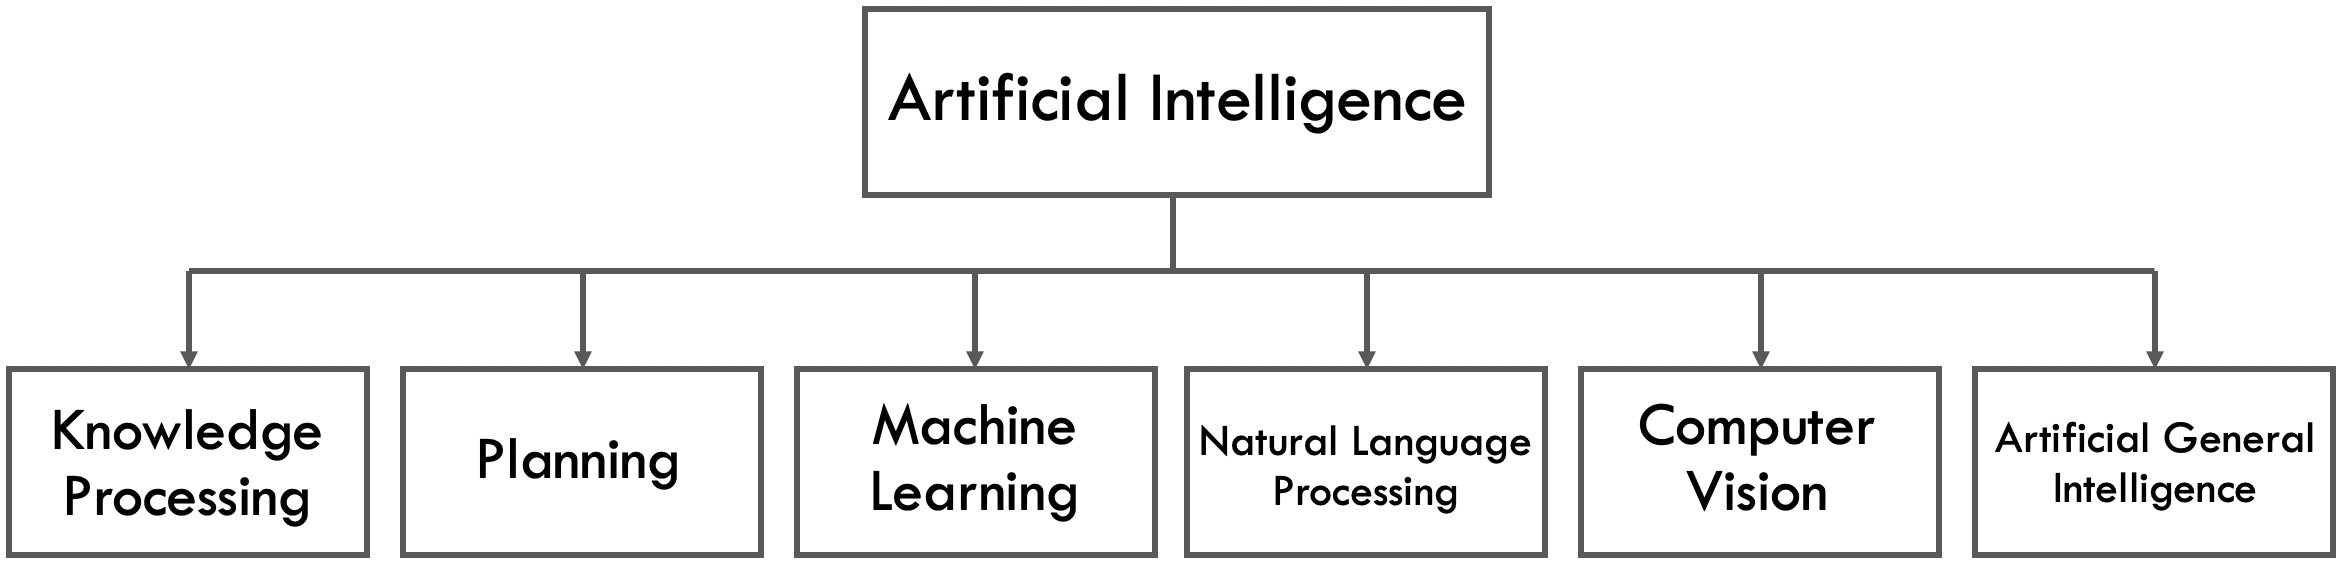
\includegraphics[width=\textwidth]{images/ch1/AIGoals.jpeg}
    \caption{The major goals of artificial intelligence.}
    \label{fig:AIGoals}
\end{figure}   

The sub-fields of ML are shown in Figure \ref{fig:MLGoals}.  In supervised learning, the algorithm learns the optimal input-output mapping, called the model, from a training data set pre-labeled by an external supervisor \cite{sutton}.  Be aware that not all labels provided are guaranteed to be correct. In fact, it is not uncommon to  have mislabeled data caused by noise in the original data set. For example, imagine trying to transcribe an interview with the audio playback heavily corrupted by noise.  In the process industry, the supervisor is typically a sensor measuring the current condition of the process (pressure, temperature, flow rate, etc.) and are often times unreliable. In the end, the performance of the supervised learning model is \textit{upper bounded} by the quality of the labels provided by the supervisor.  In the ideal case, the model can exactly replicate the right \textit{and wrong} labels of the supervisor. In unsupervised learning, the algorithms are typically used to optimally segregate data based on their similarity or to identify the principal components within large data sets \cite{Hinton, sutton}.  Objectively, unsupervised learning identifies hidden patterns within data sets through feature extraction and dimensional reduction. Semi-supervised learning is a hybrid between supervised and unsupervised learning where the models are trained on a small data set of labeled data and refined using features extracted from the unlabeled data set. For example, in the process industry, tasking an engineer to manually label data sets is a costly but required endeavor.  In many applications such as fault detection or root cause analysis, a well labeled data set is required to materialize any useful applications.  Using semi-supervised learning in these scenarios, the model can learn from the small labeled data set and extract additional helpful insights from the remaining unlabeled data to fine tune performance.  In this case, the final algorithm is vastly superior compared to its supervised or unsupervised learning counterpart \cite{machine_learning}.  Unfortunately, all the above methods exhibit one critical flaw: \textit{the inability to transcend the supervisor in terms of performance}. Although these methods may provide great cost reductions and/or greatly speed up production through automating trivial tasks, the methods fail to expand the current capabilities of modern methods.

\begin{figure}[H]
    \centering
    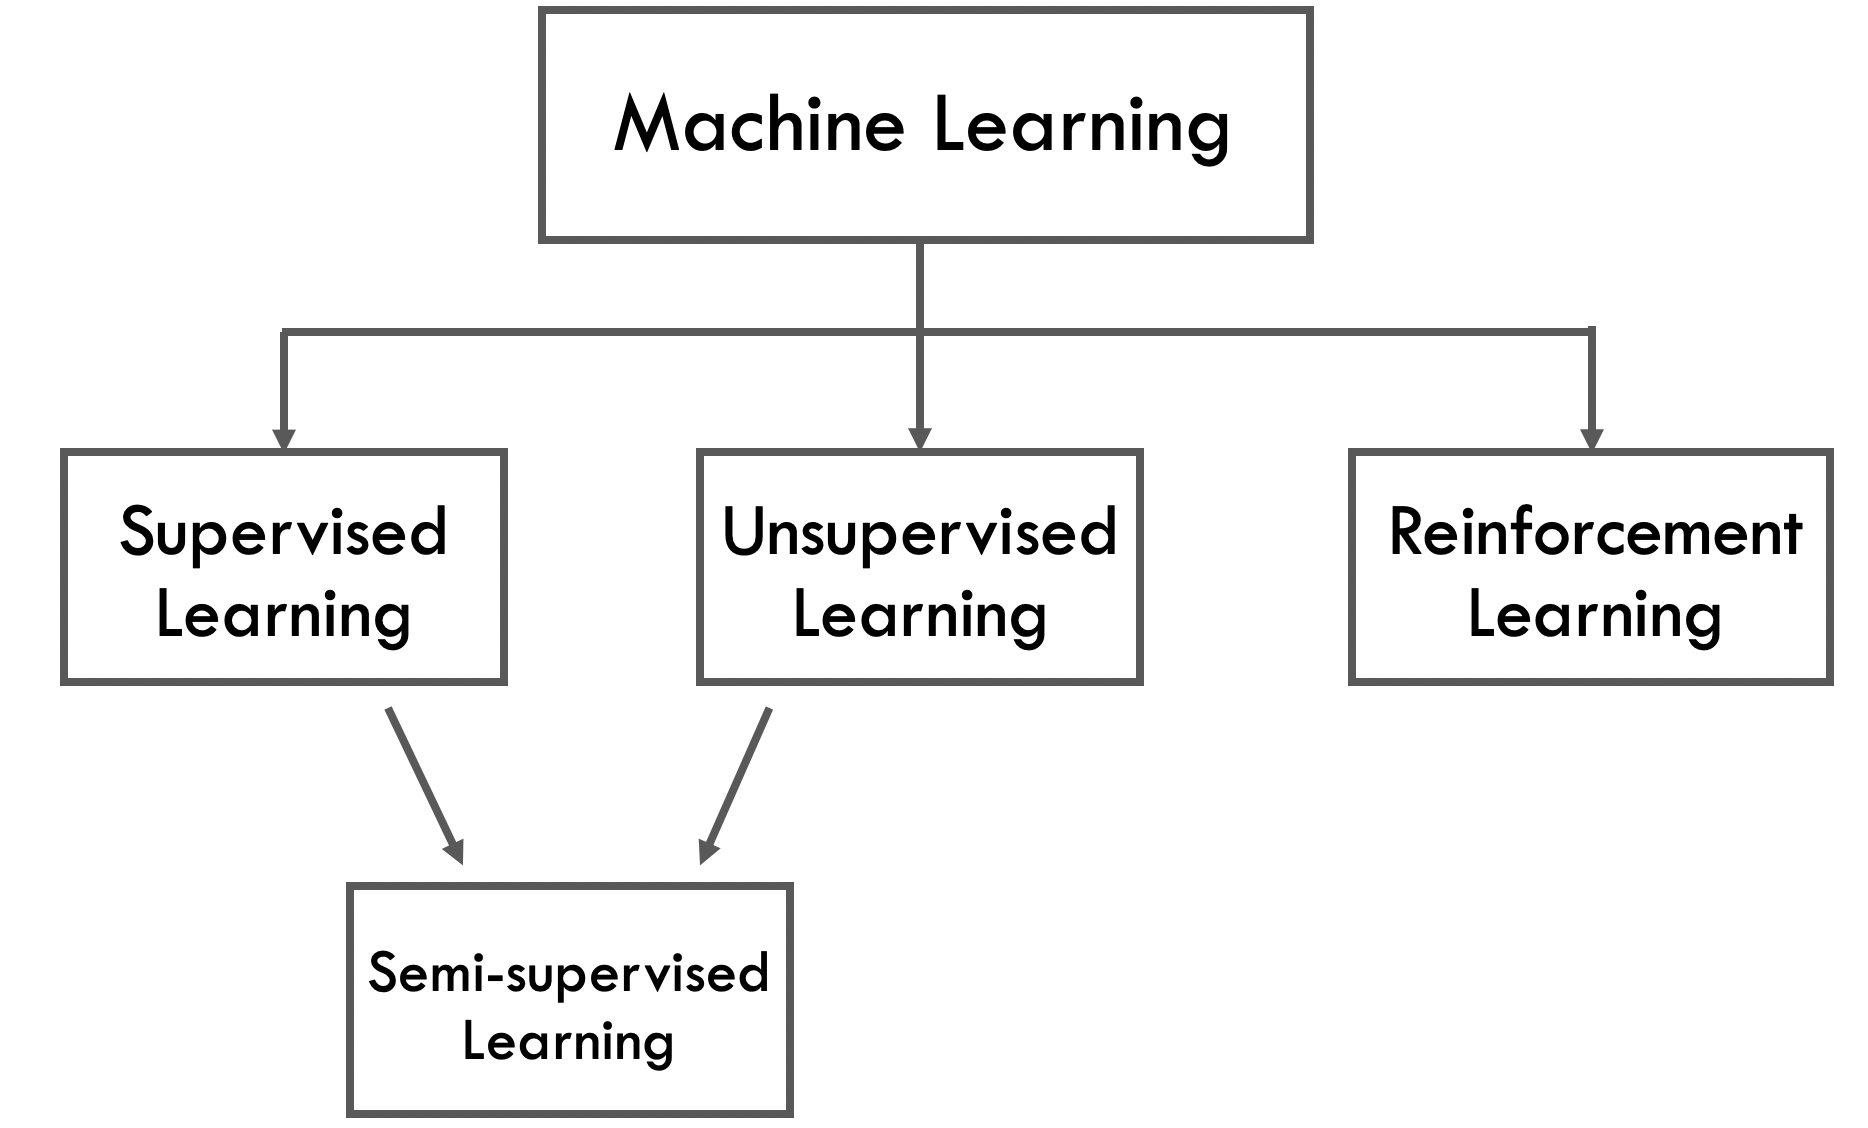
\includegraphics[width=0.6\textwidth]{images/ch1/MLGoals.jpeg}
    \caption{The sub-components of machine learning.}
    \label{fig:MLGoals}
\end{figure}   

Reinforcement learning (RL) aims to overcome this dilemma by providing machines the ability to \textit{surpass all known methods}.  More specifically, reinforcement learning \textit{agents} learns the optimal actions to perform in different situations (also called optimal policy) through self-interaction with the environment.  After each interaction, the agent is provided feedback via a scalar reward signal; large positive rewards follow good actions while negative rewards follow bad actions.  In challenging circumstances, actions affect both the immediate reward signal and the subsequent rewards there-forth. In an intuitively context, pursing an University degree may yield negative immediate rewards; however, rewards years down the line may become significantly more positive due to the newly equipped knowledge.  These two characteristics---delayed feedback and guided trial-and-error search---differentiate RL from all other types of algorithms and ultimately permit RL to push the existing boundaries of known science \cite{sutton}.


\section{Motivation and Challenges}
The non-existent price recovery of the Western Canadian Select crude index since its collapse in 2015 has forced many Canadian energy companies to shift their operating strategies from expansion to optimization \cite{oil_price}.  Typically, existing processes in the oil and gas sector are old and have been operating in a similar regime for many years.  In doing so, vast amounts of data have been collected for the current operating regime.  Through rapid advancements of computer hardware, this data can now be leveraged as a gold mine for modern data hungry machine learning algorithms.  Firstly, the data can be used for predictive applications such as forecasting, digital twinning, soft sensing, and even training purposes.  The data can also be leveraged to create "ML-assisted" safety applications similar to driver assistance in the automotive industry. For example, process monitoring and process forecasting ML models can be built to \textit{proactively} manage operational risk by identifying hazards well in advance of actual incidents. Modern optimal control methods (i.e., maximizing profits of a plant or minimizing operating cost) can also benefit greatly through the assistance of ML algorithms.  Currently, a common optimal control method is MPC; however, the method assumes the availability of an accurate process model.  In any industrial scale process, an accurate process model is nearly impossible to identify due to the vast amount of non-linear interaction effects.  Even after identification, the model would need re-tuning after several months due to process drifts and other changes. Furthermore, for large processes, the dimension of the states and actions may be too large for online optimization to be feasible. One field of study called distributed MPC aims to solve this computational hurdle by decomposing the system into smaller sub-systems; however, distributed MPC performance are typically subpar compared to its centralized counterpart due to communication issues \cite{distributed_mpc}. Through RL, such large problems may be computationally feasible as a centralized algorithm by pre-computing the optimal control policies offline. Moreover, process drifts can be naturally handled by RL through its direct adaptive optimal control nature \cite{direct_adaptive}.  For traditional optimal control, adaptive characteristics are typically indirect and require re-identification of the system models.  In the case of RL, the policy is  adapted directly through interactions with the environment. Although there exists numerous machine learning success stories in the technology sector, their applications in the process industry is still severely limited. One main reason for the absence of recent ML progress is the lack of a workforce skilled in both ML and process control.

Many technology companies and ML engineers specialized in the technology sector have attempted to fill the gap; however, process control data is exceedingly different compared to traditional image or transactional data.  The data in process control is typically unintuitive, time-series, and are often times unreliable or noisy.  There also exists many time delays in chemical processes and feature engineering is difficult without proper fundamentals of process engineering. Comparatively, the data in the technology sector is often very intuitive and easy to understand.  For example, building a classification algorithm for facial recognition is easier to understand compared to predicting when a pump will fail.  The former only requires an image of the individual or some 3D spatial data corresponding to the individual's facial features. In the latter, there may be thousands of interactions affecting the ultimate outcome of the pump, most of which are impossible to identify through intuition alone. Due to these differences, engineers not specialized in the process sector faced great challenges when attempting to create value in the process industry.

More recently, there has been a surge of ML innovations made by research scientists and AI start-up companies catered towards the process industry.  However, most were never commercialized because the mentality between industry and the engineers were vastly different.  In industry, the ultimate objective is to create shareholder value through risk-managed products; it may be traditional methods or it can be ML.  For the research scientists, the focus is more on the elegance and novelty of the algorithm, no matter the complexity. For industry, such algorithms are difficult to explain to a non-technical audience, have a high cost of ownership for the customer, and are difficult to understand without a team of subject matter experts (which themselves cost a significant amount of money).

Throughout this thesis, the main theme is to introduce easy, cost effective solutions that explicitly considers the following four customer focused values required for successful commercial products \cite{marketing}:
\begin{itemize}
    \item \textbf{Functional value:} Describes the overall usefulness of the product compared to other available products.  For example, a ML anomaly detection algorithm may be far superior compared to other methods if enough data is present.
    \item \textbf{Monetary value:} The cost savings generated from this product (e.g., amount of money saved through using an optimization algorithm or preventing a loss incident).  
    \item \textbf{Social value:} Ability for the product to enhance your brand or product awareness and is especially important for sales focused enterprises.  For example, after an individual goes to Disneyland, they may tell many people how great it was without any incentive from Disney.  In the process industry, operators and/or engineers will recommend great products that helped them in their jobs and/or become more productive without external incentives.
    \item \textbf{Psychological value:} Ability to make the company feel superior compared to the competition.  For example, a firm may believe they have better chances at winning contracts if their products contain state-of-the-art ML technology needed for big data applications.
\end{itemize}
Ultimately, the goal is to create organic growth for the local industry through new, innovative ways.  If an exceptionally complex solution is engineered, but there exists no customers, the solution didn't end up solving anything.

\section{Thesis Outline and Contributions}
The thesis is organized as follows: First, basic concepts of RL and MPC will be introduced.  In Chapter 2, applications of ML algorithms in prediction applications will be explored on an industrial pipeline.  Following that, ML for process safety applications will be shown in Chapter 3. Safety applications include topics such as anomaly detection, anomaly prediction, and alarm management. Up until Chapter 3, the projects will use exclusively traditional supervised, unsupervised, and semi-supervised learning methods because the applications are predictive in nature.  Towards the end of Chapter 3 until the end of the thesis, RL methods will be introduced because these applications are more control oriented. Chapter 4 contain various different RL applications in process control. Applications here include the optimal control of a waste water treatment plant, set point tracking control of small scale systems, and fault-tolerant control of an industrial distillation tower. Additionally, RL is also compared to MPC on simple small-scale systems in this chapter. Finally, this thesis is concluded in Chapter 5.  A comprehensive project report for the pipeline optimization project introduced throughout this thesis is shown in Appendix A.

The contributions of this thesis is as follows: In Chapter 2, methods for identifying representative process models in an industrial settings are introduced. Additionally, a new adaptive modelling method was formulated here to significantly reduce the cost of ownership of the machine learning models for the industrial partner. The adaptive method also overcomes catastrophic interference and can be retrofitted onto all model structures. Chapter 3 introduces novel data pre-processing approaches to anomaly detection and prediction in the process industry.  Additionally, a new RL-powered alarm management method is introduced for filtering of nuisance alarms, alarm reduction, and alarm prioritization.  Chapter 4 provide comparisons between traditional optimal control methods with RL on many different systems. Furthermore, a new easy-to-implement continuous non-linear RL method is also shown here.  The last contribution in Chapter 4 is the extension of RL into a fault-tolerant control where RL is used for both the fault detection algorithm and the fault tolerant controller. 


%%%%%%%%%%%%%%%%%%%%%%%%%%%%%%%%%%%%%%%%%%%%%%%%%%%%%%%%%%%%%%%%%%%%%%%%%%%%%%%%%%%%%
% Bandits
%%%%%%%%%%%%%%%%%%%%%%%%%%%%%%%%%%%%%%%%%%%%%%%%%%%%%%%%%%%%%%%%%%%%%%%%%%%%%%%%%%%%%

%%%%%%%%%%%%%%%%%%%%%%%%%%%%%%%%%%%%%%%%%%%%%%%%%%%%%%%%%%%%%%%%%%%%%%%%%%%%%%%%%%%%%
% Bandits
%%%%%%%%%%%%%%%%%%%%%%%%%%%%%%%%%%%%%%%%%%%%%%%%%%%%%%%%%%%%%%%%%%%%%%%%%%%%%%%%%%%%%

\section{Preliminaries to Reinforcement Learning}

Reinforcement learning is a goal-directed learning algorithm which continually improves its own performance through interactions with the environment \cite{sutton}. The main objectives of reinforcement learning are to identify hidden structures within the environment and to find the optimal policy (i.e., optimal state to control action mapping) through guidance from an internal scalar reward (feedback). Two distinct characteristics that deviate reinforcement learning from other methods are its trial \& error search to find the optimal policy, and its ability to identify delayed reward signals. Modern reinforcement learning methods combine principles of optimal control and learning methods together to solve for the optimal control trajectory in an environment.  In the remaining sections of this chapter, fundamental reinforcement learning concepts will be introduced.  Then, tabular based RL methods will be shown.  However, due to the "curse of dimensionality" of high dimensional problems, tabular based approaches struggle in large multi-variate scenarios.  To overcome these issues, deep neural networks will be leveraged for function approximation, and deep reinforcement learning will be introduced.

\subsection{A historical overview}
Reinforcement learning is a combination of two fields of research: \textbf{optimal control} through extremizing an objective function through dynamic programming and \textbf{animal psychology} inspiring trial-and-error search. Originally, the \textbf{optimal control} problem was proposed for designing controller to maximize or minimize the objective function of a dynamical system over time \cite{mpc}.  By the 1950s, Richard Bellman extended on the works of Hamilton and Jacobi to develop a novel approach to solve the optimal control problem.  This approach, known as dynamic programming, optimizes a system's input trajectory by using the functional equation (a function where the unknowns are also functions) generated from the system's state information together with a value function \cite{bellman1}.  The functional equation, now called the Bellman equation, is mathematically represented as:
% Will leave spaces during submission for reviewers
\begin{equation}
    V(x) = r(x) + \gamma \sum P(x' | x, u) \cdot V(x')
    \label{eq:bellman_eq}
\end{equation}
where $V(x)$ represents the value function of $x$. Here, $\gamma$ denotes the discount factor to incorporate future uncertainty. $r(x)$ is the reward signal obtained as a function of the system's desired performance. $P(x'|x, u)$ is the dynamics function describing the transitional probability of arriving at state, $x'$, given $x$ and $u$. $V(x')$ is the value function of $x'$. Intuitively, the value function describes how good or how bad being in particular state is, assuming optimal behaviour thereafter; high values represent good states and low values for bad.  True dynamic programming is "cursed by dimensionality" (i.e., computational cost increases exponentially with the dimensions of the states and actions); thus, approximate dynamic programming (ADP) methods were developed to bypass this hurdle \cite{adp}.  In reinforcement learning, many ADP methods are leveraged to solve for the optimal policy. The concept of a feedback oriented learning system in RL originated from \textbf{animal psychology}. More specifically, the original concept was introduced in the early $20^{th}$ century, named the "Law of Effect". The law stated that animals tend to repeat actions resulting in good outcomes, vice versa for actions with bad outcomes \cite{thorndike}. Initially, the agent explores the environment in which it exists to identify the outcomes corresponding to different actions, then only repeating the actions resulting in good outcomes thereafter. By unifying dynamic programming from optimal control and trial-and-error search from animal psychology, the modern field of RL was developed. For a more comprehensive overview of the history of RL, see \cite{sutton}.

The development of RL is shown in Table \ref{tab:RLevo}.  Reinforcement learning takes its roots from the \textit{k}-armed bandit problem that has been extensively studied in engineering, psychology, and statistics.  This problem disregards state information, and only worries about solving the optimal actions for \textit{one} specific situation \cite{thompson1, thompson2, robbins, bellman_bandit}.  As a natural extension, Barto, Sutton and Brouwer expanded the idea to multi-situation systems \cite{bartosuttonbrouwer} through associative search, also known as \textit{contextual bandits}. The main objective of this algorithm was to find an optimal policy, $\pi^*(x)$, for each situation.  However, it only concerns the immediate rewards and not the long term consequences. Reinforcement learning was then developed to find the optimal policy for different situations based on immediate reward and the onward trajectory there-forth.  

\begin{table}[H]
\caption{From left to right, the evolution of reinforcement learning.}
\centering
\begin{tabular}{c|c|c}
\textbf{$k$-armed bandits}	& \textbf{Contextual bandits}	& \textbf{Reinforcement learning}\\
\hline
Optimal action		  & Optimal action			& Optimal action \\
One situation		  & Many situations			& Many situations \\
Immediate consequence & Immediate consequence	& Long-term consequence \\
\end{tabular}
\label{tab:RLevo}
\end{table}

\subsubsection{\textit{k}-armed Bandit}

The \textit{k}-armed bandit problem provides the fundamentals to understanding modern reinforcement learning.  Here, an agent is present and must choose action $u$ from $\mathcal{U}$, where $\mathcal{U}$ has $k$ choices.  After each action, a scalar reward from a stationary distribution will be returned to the agent as feedback. Favorable actions yield positive rewards, while unfavorable actions return negative rewards. The objective of the agent is to ultimately maximize reward over $N$ steps.  For each action, there is an expected reward called \textit{value}, given by Equation \ref{eq:01value}.

\begin{equation}
    \centering
    q_*(u) = \mathbb{E}[R_t | U_t = u]
    \label{eq:01value}
\end{equation}
where $u$ is the action taken at time, $t$.  $R_t$ is a scalar reward returned to the agent after action $u$ was performed at time $t$. $R_t$ is drawn from a stationary distribution, $R_t \thicksim N(q_*(u), \sigma^2)$. Finally, $q_*(u)$ is the expected reward of taking action, $u$.

The real value is unknown, however, an estimation can be computed and is denoted as $Q_t(u)$.  Given all $Q_t(u)$ is maintained, at any time, one $Q_t(u)$ will be greater than all others. Picking the action that corresponds to the maximum $Q_t(u)$ is known as \textit{greedy}, and the agent is said to be \textit{exploiting}.  If a non-maximum action is picked, the agent is \textit{exploring} \cite{sutton}.

Action selection based on estimating the value of actions are called \textbf{Action-value methods} \cite{action_value_method}. At time $t$, the estimate of the value is given by Equation \ref{eq: value_est} \cite{sutton}.

\begin{equation}
    \centering
    Q_t(u) = \
    = \frac{\sum_{i=1}^{t - 1} R_i \mathbbm{1}_{U_i=u}}
    {\sum_{i = 1}^{t - 1} \mathbbm{1}_{U_i = u}}
    \label{eq: value_est}
\end{equation}
where $\mathbbm{1}$ equals 1 if the condition is true, else 0.  $R_i$ is the reward obtained at the $i^{th}$ episode through selecting action, $U_i$.  Intuitively, the numerator is the sum of rewards when action, $u$, was taken prior to $t$.  Likewise, the denominator is the number of times action, $u$, was taken prior to $t$. As $t \rightarrow \infty$, $Q_t(u) \rightarrow q_*(u)$.  Action selection is based on Equation \ref{eq: bandit_action_selection}.

\begin{equation}
    \centering
    U_t = \argmax_u Q_t(u)
    \label{eq: bandit_action_selection}
\end{equation}

However, initial successful episodes may cause the agent to be stuck at local minimums. To overcome this, a semi-stochastic action selection method called $\epsilon$-greedy can be introduced to promote exploration. In this method, the agent will perform a random action with $\epsilon$ probability (greedy action can be performed).  Higher $\epsilon$ results in more exploratory moves.  Consequently, all $u \in \mathcal{U}$ will be picked many times and by the law of large numbers, $Q_t(a) \rightarrow q_*(a)$ \cite{large_numbers}. Figure \ref{fig: eps_figure} shows the effect of $\epsilon$ on the performance of the agent.

\begin{figure}[H]
    \centering
    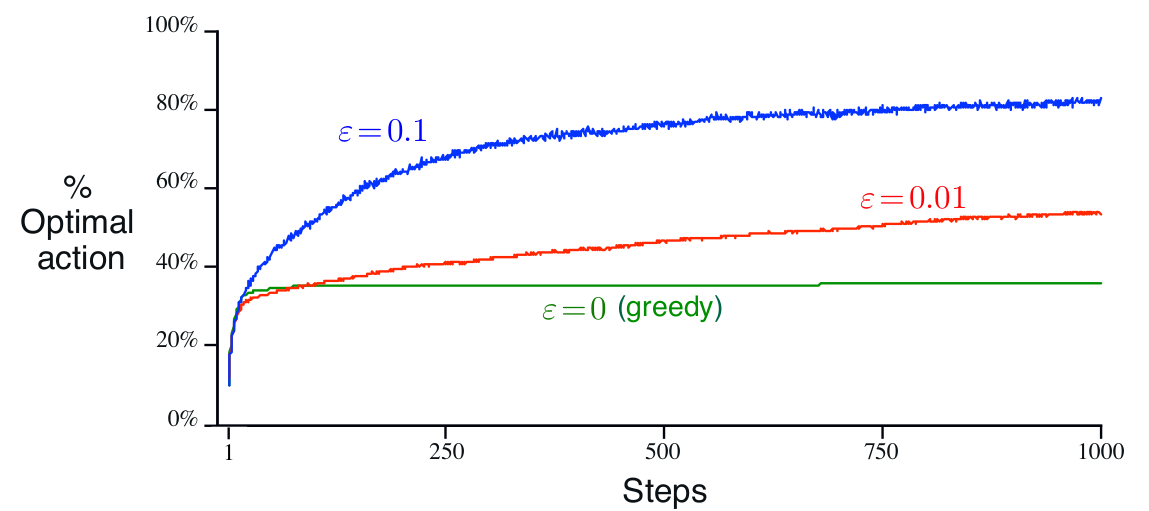
\includegraphics[scale=0.35]{images/eps_vs_optAction.png}
    \caption{Average performance of three agents using different $\epsilon$.  The data is averaged over 2000 runs.  Figure from \textit{Reinforcement Learning: An Introduction} by Sutton and Barto (2018).}
    \label{fig: eps_figure}
\end{figure}

During implementation, $\epsilon$ should decay out as $Q_t(a)$ approaches $q_*(a)$ to ensure knowledge of the agent is being adequately exploited. For non-stationary problems, $\epsilon > 0 \; \forall t$ to ensure other action values have not changed.

Algorithms to solve the \textit{k}-armed bandit problem are easily applied to situations where the concept of state is inert and only the actions are of concern;  a near impossibility in the real world.  

\subsubsection{Contextual Bandit}

A natural extension of the \textit{k}-armed bandit is associative search.  In associative search (sometimes called contextual bandit), different policies are associated with different situations \cite{bartosuttonbrouwer}.  Equation \ref{eq: state-action-value} is the extension of Equation \ref{eq:01value} in the associative search problem.

\begin{equation}
    \centering
    q_*(x, u) = \mathbb{E}[R_t | X_t = x, U_t = u]
    \label{eq: state-action-value}
\end{equation}

Associative search is known as the method between \textit{k}-armed bandits and reinforcement learning.  In associative search, the objective is to associate optimal policies to different situations, but only maximizing the \textit{immediate} reward.  Often times, near term sacrifices are required to initiate the trajectory to a large lump sum reward at the terminal state.  For example, heavy capital and time investment is required for University in the short term.  However, the long term gain is so great that it outweighs the short term losses, making going to University an optimal policy for many individuals.

In order to find the true optimal policy (i.e., policy that returns the greatest rewards over a long time period), the topic of reinforcement learning is developed.  In reinforcement learning, sequential decision making is explored to identify the delayed reward signals from different actions and to ultimately find the optimal policy, $\pi^*$.  

%%%%%%%%%%%%%%%%%%%%%%%%%%%%%%%%%%%%%%%%%%%%%%%%%%%%%%%%%%%%%%%%%%%%%%%%%%%%%%%%%%%%%
% MARKOV DECISION PROCESSES
%%%%%%%%%%%%%%%%%%%%%%%%%%%%%%%%%%%%%%%%%%%%%%%%%%%%%%%%%%%%%%%%%%%%%%%%%%%%%%%%%%%%%

%%%%%%%%%%%%%%%%%%%%%%%%%%%%%%%%%%%%%%%%%%%%%%%%%%%%%%%%%%%%%%%%%%%%%%%%%%%%%%%%%%%%%
% MARKOV DECISION PROCESSES
%
% Introduction to MDPs, finite MDPs, infinite MDPs
% Semi MDPs
% Partially Observable MDPs
%
%%%%%%%%%%%%%%%%%%%%%%%%%%%%%%%%%%%%%%%%%%%%%%%%%%%%%%%%%%%%%%%%%%%%%%%%%%%%%%%%%%%%%

\section{Markov Decision Processes}
In the face of uncertainty, the agent's \textit{sequential} decision making is formalized in the Markov decision process (MDP). The general MDP framework is shown in Figure \ref{fig:01mdp} and contains two components: the \textbf{agent} and the \textbf{system}. The \textbf{agent} is a continuously learning decision maker and is mathematically represented by the RL algorithm. Objectively, the agent will undergo numerous meaningful interactions with the system to ultimately learn the optimal policy, $\pi^*$ (i.e., the optimal decisions given different situations). Conversely, the \textbf{system} contains all elements the agent cannot arbitrarily control. In process control, the ambient temperature, actuators, and even the wires transporting the control signals are all part of the system because the agent cannot \textit{deterministically} manipulate them. 

\begin{figure}[H]
    \centering
    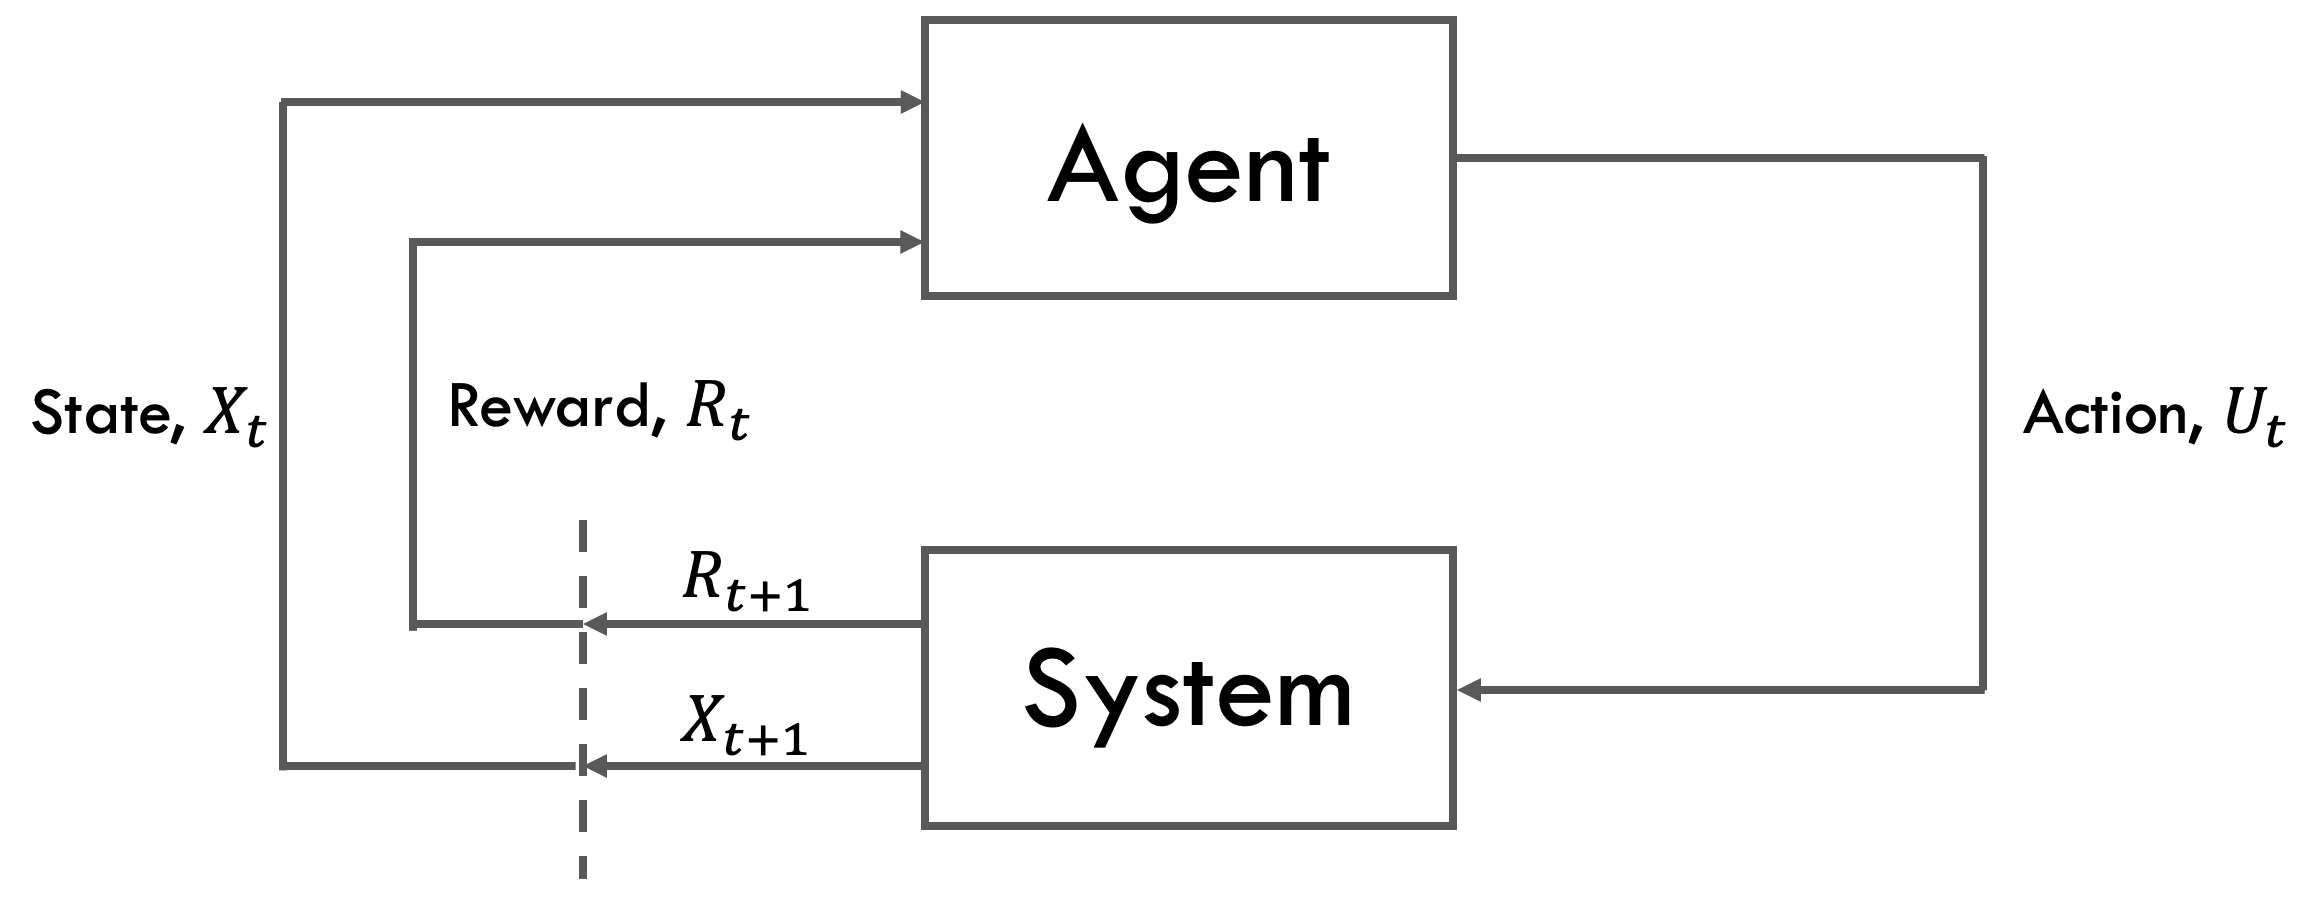
\includegraphics[width=0.56\textwidth]{images/ch1/MDP.jpeg}
    \caption{The general Markov decision process framework. Original image from \cite{sutton}.}
    \label{fig:01mdp}
\end{figure}   

Mathematically, the MDP is a discrete representation of the stochastic optimal problem and a classical formulation of \textit{sequential} decision making where both the immediate and long term consequences are explicitly considered \cite{bellman1, mdp_bellman}. Many definitions of the MDP exist and are equivalent up to small alterations of the process.  One comprehensive definition is that a MDP is a tuple $\mathcal{M}$, is a tuple $(\mathcal{X}, \mathcal{U}$, $P(x', r|x, u), \gamma, R)$ comprised of the following\cite{ng_ref12}:
\begin{itemize}
    \item $x \in \mathcal{X}$: \textbf{State} space of the system at each time step. Common states in industrial processes include temperatures, valve positions, pressures, flow rates, etc.
    \item $u \in \mathcal{U}$: Bounded \textbf{action} space of the agent, ($\mathcal{U}$ $ \geq 2 $). In traditional control, this is the \textbf{bounded input signals} sent to the actuators.
    \item $R \in \mathbb{R}$: Expected \textbf{reward} signal after performing action $u$ in state $x$. Reward functions are designed based on a desired performance metric.  In control theory, the reward function is known as the \textbf{objective function}.  Typically, $|R| \leq \mathcal{R}$ for convergence guarantees.
    \item $p(x', r|x, u)$: Systems \textbf{dynamics function}. Formally, it is the probability of transitioning to $x'$ and receiving $r$,  given states $x \in \mathcal{X}$ and performing action $u \in \mathcal{U}$. Mathematically, it is described by the following:
    \begin{equation}
        p(x', r | x, u) \dot{=} Pr\{X_t = x', R_t = r | X_{t - 1} = x, U_{t-1} = u\}
        \label{eq:transition_prob}
    \end{equation}
    where $p$ describes the system \textbf{dynamics} and $Pr$ denotes the probability operation \cite{sutton}. Additionally, $p$ satisfies the following equality:
    \begin{equation}
        \sum\limits_{x' \in \mathcal{X}} \sum\limits_{r \in \mathcal{R}} p(x', r | x, u) = 1, \forall x \in \mathcal{X}, u \in \mathcal{U}
        \label{eq:prob}
    \end{equation}
    Notice here that $p$ is only a function of the \textit{immediate past}, thus assuming that $x_{t - 1}$ and $u_{t-1}$ captures the complete history. This is known as the Markov property and its underlining assumptions are critical for successful process control applications using RL. Additionally, note that when the state and actions are formulated as augmented past information: $x_{t-1} = [s_{t-1}, s_{t-2}, ... s_{t-N}], u_{t-1} = [a_{t-1}, a_{t-2}, ..., a_{t-N}]$, where $s_{t-N}$ and $a_{t-N}$ denotes the past states and actions, the system is still Markov because decisions can be made exclusively using $x_{t-1}$ and $u_{t-1}$. 
    \item $\gamma$: \textbf{Discount factor} associated with uncertainty of the future, ($0 \leq \gamma \leq 1)$. $\gamma < 1$ is also a requirement for continuous processes to guarantee eventual convergence.
\end{itemize}

There exists three different MDPs: fully observable MDP (FOMDP), partially observable MDP (POMDP), and semi MDP (SMDP). Table \ref{tab:01mdps} shows a general guideline on the different MDPs.

\begin{table}[H]
\caption{A comparison of different Markov decision processes.}
\centering
\begin{tabular}{c|c|c}
\textbf{FO-MDPs}	& \textbf{S-MDPs}	& \textbf{PO-MDPs}\\
\hline
All states observable		  & All states observable			& Some states observable \\
Discrete time		          & Continuous time	             	& Discrete time \\
\end{tabular}
\label{tab:01mdps}
\end{table}

\subsection{Fully observable Markov decision processes}
Fully observable Markov decision processes are the simplest and serves as the foundational framework.  They are mainly applied to discrete systems with fixed sampling times where transition dynamics are unimportant and all states are observable (measurable in control literature). Here, the agent starts in some initial states, $x_0$. At each time $t$, the agent maps $x_t$ to some $u_t$ corresponding to its policy, $\pi_t$.  Given $x_t$ and $u_t$, the system will then transition to some new states $x_{t+1}$ dictated by Equation \ref{eq:transition_prob} while outputting reward signal $R_{t+1}$ based on the reward function. In regulation and set-point tracking problems, this reward function is typically the squared tracking error between $x_t$ and $x_{sp}$.  By repeating this cycle many times, the agent is able to traverse through some sequence, $x_t, u_t, R_{t+1}, x_{t+1}, u_{t+1}, R_{t+2}, x_{t+3}, ...$ and accumulate \cite{sutton}:
\begin{align}
G_t &= R_{t+1} + \gamma R_{t+2} + \gamma^2 R_{t+3} ... \\
    &= \sum\limits^{\infty}_{k = 0} \gamma^k R_{t+k+1}
\label{eq:return}
\end{align}
where $G_t$ denotes the cumulative discounted return at time $t$ and $\gamma$ is the discount factor to capture the future uncertainty. MDPs can represent both finite or infinite systems; the former describes episodic tasks with explicit terminal states while the latter describes tasks that continue forever.  Intuitively, most two-player board games such as Checkers, Chess, or Go are finite MDPs where the game is terminated after one player is defeated.  Contrarily, an infinite MDP system could be the control system in an industrial process. For infinite MDP systems, $\gamma < 1$ is a necessary condition to keep $G_t$ bounded. Ultimately, the agent is tasked with finding the optimal policy, $\pi^*$, that maximize $G_t$, and subsequently the value function, over $N$ steps. The value function for each state is given as \cite{sutton}:
\begin{align}
    v_\pi (x) &\dot{=} \mathbb{E}_\pi [G_t | X_t = x] \\
              &= \mathbb{E}_\pi \left[\sum\limits^\infty_{k=0} \gamma^k R_{t+k+1} | X_t = x \right] \\
              &= \mathbb{E}_\pi [R_{t+1} + \gamma G_{t+1} | X_t = x]
    \label{eq:value_func}
\end{align}
where $v_\pi (x)$ is the value function of $x$ under policy $\pi$. Theoretically, the existence and uniqueness of $v_{\pi}$ is guaranteed for continuous systems where $\gamma < 1$ or in systems with guaranteed termination.  Compared to Equation \ref{eq:01value}, Equation \ref{eq:value_func} takes the expectation of $G_t$; therefore, explicitly optimizing the long term returns rather than only the immediate rewards. The action-value formulation of Equation \ref{eq:value_func} is:
\begin{align}
    q_\pi (x, u) \; &\dot{=} \; \mathbb{E}_\pi [G_t | X_t = x, U_t = u] \\
                 &= \mathbb{E}_\pi \left[\sum\limits^\infty_{k=0} \gamma^k R_{t+k+1} | X_t = x, U_t = u \right], \forall x, u \in \mathcal{X, U}
    \label{eq:a_value_func}
\end{align}
FOMDPs work well for discrete systems where all states are observable.  However, system states in industrial processes are often unobservable (unmeasurable in control) due to limited hardware or engineering limitations. In such systems, the Markov property no longer holds resulting in sub-optimal decision making of the agent.





\subsection{Partially observable Markov decision processes}
Partially observable Markov decision processes (POMDPs) extend upon the concepts of FOMDPs and represent systems with unobservable states. In RL literature, observability is equivalent to measurability in control; thus, the two terms are used interchangeably here-forth. In FOMDPs, the current state $x_t$ at each time $t$ is fully observable. In the more general setting of POMDPs, the entire state vector describing the agent's current situation is no longer available. Instead, the agent only has access to a set of possible observations $\mathcal{O}$. At each time $t$, the agent sees observation $o_t$ which correspond to probability distributions over states.  Using $o_t$, the agent can infer the states it \textit{might} currently be in \cite{ng_ref12}. Relating to a process control setting, existing sensors typically only measure a subset of the current states; however, by using available measurements, one can infer the remaining unmeasurable states using probabilistic approaches.

Generally, finding $\pi^*$ in a POMDP setting is significantly harder compared to FOMDPs.  Even finding a near-optimal policy is at least NP-hard (non-deterministic polynomial time) \cite{pomdp_time}.  Furthermore, even agents with access to all the system's true value functions are unable to behave optimally in a POMDP setting because the current states are unknown \cite{ng_ref12}. 

Belief states is one method for agents to behave optimally in POMDPs. On a high level, belief states transform the POMDP setting into its FOMDP counterpart through a probabilistic approach. Specifically, belief states, $b$, are probability distributions over states deduced using previous observations and actions. The probability distributions represent what the agent thinks its current state is. Using these probabilities, the agent can compute scalar value functions of each state-action pair and use these to act "optimally".  Note here that the agent's behaviour is optimal given the available information, and not optimal with respect to the system. An quantitative example is provided below:
\begin{quote}
    Suppose an agent exists in a two-input two-output (TITO) POMDP setting with two unobservable states ($x_1$ and $x_2$) and two actions ($u_1$ and $u_2$) and suppose the problem is only concerned with the immediate consequences (for longer horizons, the agent must also consider the long term rewards, making the example less intuitive). In this system, there are four value functions, one for each state-action pair. Suppose $u_1$ earns a reward of 2 in $x_1$ and 0 in $x_2$.  Similarily, $u_2$ earns a reward of 0 in $x_1$ and 1 in $x_2$.  Given $b_t = [0.2, 0.8]$ (probabilities of being in $x_1$ and $x_2$, respectively), then $Q(b_t, u_1) = 0.2 \cdot 2 + 0.8 \cdot 0 = 0.4$ and $Q(b_t, u_2) = 0.2 \cdot 0 + 0.8 \cdot 1 = 0.8$, resulting in $u_2$ being the optimal action.
\end{quote}

In control theory, observers, such as soft sensors, are used to estimate unmeasurable states.  Observers are typically $1^{st}$ principles, data driven, or probabilistic models. The concept of belief states is very similar to observer design in control theory. Traditionally, Kalman filter is a widely used observer design. Conversely, recurrent neural networks (RNNs) are widely used for belief state estimation in RL. The performance of RNN was compared with Kalman filter in \cite{RNNvsKF}, drawing similarities of the two methods' objective, theory, and performance.

System representations using FOMDPs and POMDPs work well in discrete tasks where transition times are constant and transition dynamics are disregarded; however, both topics are paramount for continuous optimal control.  







\subsection{Semi Markov decision processes}
Typical MDPs are discrete representations of the optimal control problem and are sub-optimal in continuous tasks. Semi-Markov decision processes (SMDP) are an extension of MDPs to continuing tasks with unknown transition times and system dynamics. In SMDPs, the transition dynamics of the system are explicitly captured using reward function \cite{continuous_rl_ref14}:
\begin{equation}
R(x_t, x_{t+1}, u_t) = \int\limits^\infty_0 \int\limits^t_0 e^{-\beta s} \rho(x_t, \pi (x_t))dsdF_{x_t, x_{t+1}}(t | \pi (x_t))
\label{eq:reward_rate}    
\end{equation}
where $R(x_t, x_{t+1}, u_t)$ is the expected reward to be received when transitioning from $x_t$ to $x_{t+1}$ after action $u_t$. The rewards, $R$, are calculated at each time step in the transition period to explicitly capture transition information. Then, the average reward of the transition is used to update the agent. Here, $\rho(x_t, \pi(x_t))$ represents the average reward during the transition following policy, $\pi$. $F_{x, x_{t+1}}(t, u)$ denotes the probability distribution of the time required to transition from $x_t$ to $x_{t+1}$.  Finally, $\beta > 0$ denotes the \textit{constant} discount factor in SMDPs, where higher $\beta$ results in short-sighted agents. In SMDPs, the discount factor is corrected for transition time during each update step.  The corrected discount factor is given by:
\begin{equation}
    \gamma(x_t, x_{t+1}, u) = \int\limits^{\infty}_0 e^{-\beta t} dF_{x_t, x_{t+1}}(t | \pi_t)
\end{equation}
where $\gamma (x_t, x_{t+1}, u_t)$ is the expected discount factor that will be applied to the value of state $x_{t+1}$ during the update step shown in Equation \ref{eq:bellman_eq}. The value function for SMDPs is obtained from combining Equations \ref{eq:reward_rate} and \ref{eq:value_func}:
\begin{equation}
v_{\pi}(x_t) = \frac{1 - e^{-\beta \tau}}{\beta} R(x_t, x_{t+1}, \pi(x_t)) + e^{-\beta \tau}v_{\pi}(x_{t+1})
\end{equation}
where $\tau$ is the unknown transition time.  Similarily, the action-value form is given by:
\begin{equation}
    q_{\pi}(x_t, u_t) = \frac{1 - e^{-\beta \tau}}{\beta} R(x_t, x_{t+1}, \pi(x_t)) + e^{-\beta \tau}  q_{\pi}(x_{t+1}, u_{t+1})
\end{equation}
By representing control problems as SMDPs, control strategies resulting in large overshoot, inverse response, or any other undesirable dynamics behaviour can be minimized. Additionally, the system will be able to handle systems with unknown transition times.  An intuitive example illustrating the advantages of SMDPs in process control is as follows:

\begin{quote}
    Suppose a refinery company is operating a continuously stirred tank reactor (CSTR). Objectively, the CSTR must maintain 200$^{\circ}$ C for optimal performance.  The temperature is controlled through a heat exchanger using cold water.  A RL agent was built to optimally control the flow of cold water to maintain the temperature set point. Suppose the CSTR starts at 220$^{\circ}$ C.  Agents using MDP representations may be overly aggressive and send large input signals because the reward is only calculated \textit{right before} the next evaluation step. Therefore, input signals resulting in large overshoot or inverse response may not be reflected in the reward. Contrarily, SMDP representation uses the average reward accumulated along the trajectory to provide feedback to the agent, allowing the transition dynamics to be explicitly captured. This way, input signals resulting in undesirable behaviour can be captured and mitigated. Furthermore, SMDP representations can have flexible evaluation times (traditional representations evaluate after a set time period), enabling re-evaluation during the transitional period and adjusts the discount factor in accordance to the elapsed time from last evaluation.
\end{quote}









\subsection{Optimal solution of the Markov decision processes}
The optimal solution to the RL problem refers to identifying a policy that generates the highest long term returns. Such a policy may not be unique; there may exist many optimal policies, where $v_{\pi^*_1} = v_{\pi^*_2} = ... = v_{\pi^*_N}$.  Formally, the optimal policy must satisfy the \textbf{principle of optimality}: the optimal policy $\pi^*$ is optimal if and only if $v_{\pi^*}(x) \geq v_{\pi \neq \pi^*}(x)$ for all $x \in \mathcal{X}$ \cite{PO}. Mathematically, the optimal value function is:
\begin{equation}
    v^*(x) \dot{=} \argmax_{\pi} v_{\pi}(x), \forall x \in \mathcal{X}
\end{equation}
with its action-value variant being:
\begin{equation}
    q^*(x, u) \dot{=} \argmax_{\pi} q_{\pi}(x, u), \forall x, u \in \mathcal{X, U}
\end{equation}
In a more explicit form, the optimal value function and action-value function written in terms of Equations \ref{eq:value_func} and \ref{eq:a_value_func} are given, respectively, by \cite{sutton}:
\begin{equation}
    v^*(x) = \argmax_{u} \mathbb{E}[R_{t+1} + \gamma v^*(X_{t+1}) | X_t = x, U_t = u]
    \label{eq:01valuefunc}
\end{equation}
\begin{equation}
    q^*(x, u) = \mathbb{E}\left[R_{t+1} + \gamma \argmax_{u_{t+1}} q^*(X_{t+1}, u_{t+1}) | X_t = x, U_t = u \right]
\end{equation}
Here, the $max$ operation denotes that the optimal action will be taken for the remaining of the trajectory. Theoretically, all optimal value functions can be explicitly solved using Equation \ref{eq:01valuefunc}; however, such a task would require unreasonable amounts of computation power for even simple systems. In the following section, three popular methods will be introduced to estimate the value and action-value functions in reinforcement learning.


%%%%%%%%%%%%%%%%%%%%%%%%%%%%%%%%%%%%%%%%%%%%%%%%%%%%%%%%%%%%%%%%%%%%%%%%%%%%%%%%%%%%%
% Reinforcement Learning
%%%%%%%%%%%%%%%%%%%%%%%%%%%%%%%%%%%%%%%%%%%%%%%%%%%%%%%%%%%%%%%%%%%%%%%%%%%%%%%%%%%

%%%%%%%%%%%%%%%%%%%%%%%%%%%%%%%%%%%%%%%%%%%%%%%%%%%%%%%%%%%%%%%%%%%%%%%%%%%%%%%%%%%%%
% Reinforcement Learning
%
% Introduction to MDPs, finite MDPs, infinite MDPs
% Semi MDPs
% Partially Observable MDPs
%
%%%%%%%%%%%%%%%%%%%%%%%%%%%%%%%%%%%%%%%%%%%%%%%%%%%%%%%%%%%%%%%%%%%%%%%%%%%%%%%%%%%

\section{Introduction to Reinforcement Learning}

Reinforcement learning is a goal-directed learning algorithm which continually improves its own performance through interactions with the environment \cite{sutton}. The main objectives of reinforcement learning are to identify hidden structures within the environment and to find the optimal policy (i.e., optimal input trajectory) through guidance from an internal scalar reward (feedback). Two distinct characteristics that deviate reinforcement learning from other methods are its trial \& error search to find the optimal policy, and its ability to identify delayed reward signals. Modern reinforcement learning methods combine principles of optimal control and learning methods together to solve for the optimal control trajectory in an environment.  In this chapter, fundamental reinforcement learning concepts are first introduced.  Then, tabular based methods will be shown.  However, due to the "curse of dimensionality" of high dimensional problems, tabular based approaches fail to bear fruit.  To overcome these issues, deep neural networks will be used for function approximation, and deep reinforcement learning will be introduced.

Reinforcement learning takes its roots from the \textit{k}-armed bandit problem that has been extensively studied in engineering, psychology, and statistics.  This problem disregards state information, and only worries about solving the optimal actions for \textit{one} specific situation \cite{thompson1, thompson2, robbins, bellman_bandit}.  As a natural extension, Barto, Sutton and Brouwer expanded the idea to multi-situation systems \cite{bartosuttonbrouwer} through associative search, also known as \textit{contextual bandits}. The main objective of this algorithm was to find an optimal policy, $\pi^*(x)$, for each situation.  However, it only concerns the immediate rewards and not the long term consequences. Reinforcement learning was then developed to find the optimal policy for different situations based on immediate reward and the onward trajectory there-forth.  

\subsubsection{\textit{k}-armed Bandit}

The \textit{k}-armed bandit problem provides the fundamentals to understanding modern reinforcement learning.  Here, an agent is present and must choose action $u$ from $\mathcal{U}$, where $\mathcal{U}$ has $k$ choices.  After each action, a scalar reward from a stationary distribution will be returned to the agent as feedback. Favorable actions yield positive rewards, while unfavorable actions return negative rewards. The objective of the agent is to ultimately maximize reward over $N$ steps.  For each action, there is an expected reward called \textit{value}, given by Equation \ref{eq: value}.

\begin{equation}
    \centering
    q_*(u) = \mathbb{E}[R_t | U_t = u]
    \label{eq: value}
\end{equation}
where $u$ is the action taken at time, $t$.  $R_t$ is a scalar reward returned to the agent after action $u$ was performed at time $t$. $R_t$ is drawn from a stationary distribution (typically Gaussian), $R_t \thicksim N(q_*(u), \sigma^2)$. Finally, $q_*(u)$ is the expected reward of taking action, $u$.

The real value is unknown, however, an estimation can be computed and is denoted as $Q_t(u)$.  Given all $Q_t(u)$ is maintained, at any time, one $Q_t(u)$ will be greater than all others. Picking the action that corresponds to the maximum $Q_t(u)$ is known as \textit{greedy}, and the agent is said to be \textit{exploiting}.  If a non-maximum action is picked, the agent is \textit{exploring} \cite{sutton}.

Action selection based on estimating the value of actions are called \textbf{Action-value methods} \cite{action_value_method}. At time $t$, the estimate of the value is given by Equation \ref{eq: value_est} \cite{sutton}.

\begin{equation}
    \centering
    Q_t(u) = \
    = \frac{\sum_{i=1}^{t - 1} R_i \mathbbm{1}_{U_i=u}}
    {\sum_{i = 1}^{t - 1} \mathbbm{1}_{U_i = u}}
    \label{eq: value_est}
\end{equation}
where $\mathbbm{1}$ equals 1 if the condition is true, else 0.  $R_i$ is the reward obtained at the $i^{th}$ episode through selecting action, $U_i$.  Intuitively, the numerator is the sum of rewards when action, $u$, was taken prior to $t$.  Likewise, the denominator is the number of times action, $u$, was taken prior to $t$. As $t \rightarrow \infty$, $Q_t(u) \rightarrow q_*(u)$.  Action selection is based on Equation \ref{eq: bandit_action_selection}.

\begin{equation}
    \centering
    A_t = \argmax_a Q_t(u)
    \label{eq: bandit_action_selection}
\end{equation}

However, initial successful episodes may cause the agent to be stuck at local minimums. To overcome this, a semi-stochastic action selection method called $\epsilon$-greedy can be introduced to promote exploration. In this method, the agent will perform a random action with $\epsilon$ probability (greedy action can be performed).  Higher $\epsilon$ results in more exploratory moves.  Consequently, all $u \in \mathcal{U}$ will be picked many times and by the law of large numbers, $Q_t(a) \rightarrow q_*(a)$ \cite{large_numbers}. Figure \ref{fig: eps_figure} shows the effect of $\epsilon$ on the performance of the agent.

\begin{figure}[h]
    \centering
    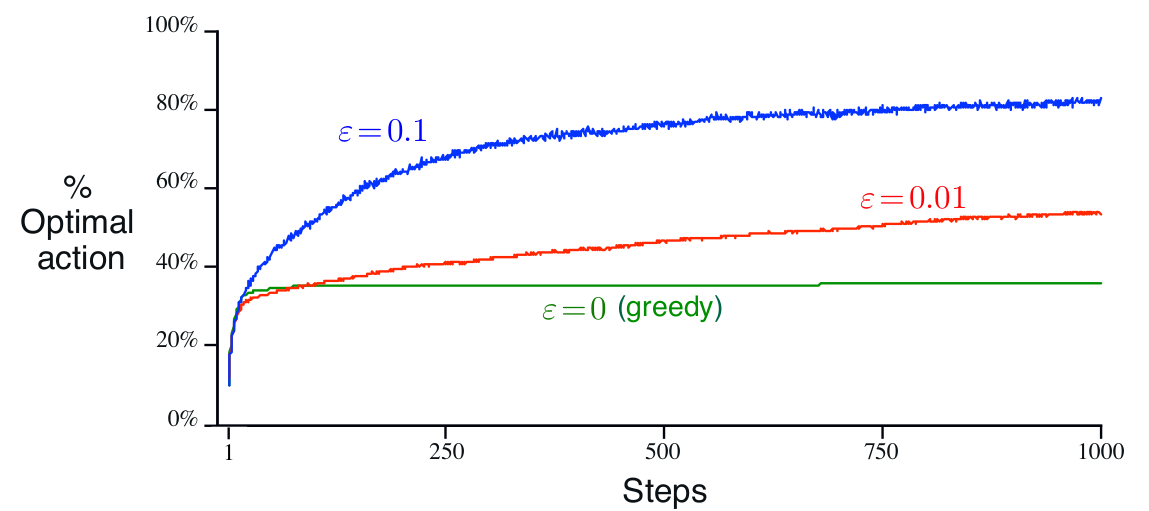
\includegraphics[scale=0.35]{images/eps_vs_optAction.png}
    \caption{Average performance of three agents using different $\epsilon$.  The data is averaged over 2000 runs.  Figure from \textit{Reinforcement Learning: An Introduction} by Sutton and Barto (2018).}
    \label{fig: eps_figure}
\end{figure}

During implementation, $\epsilon$ should decay out as $Q_t(a)$ approaches $q_*(a)$ to ensure knowledge of the agent is being adequately exploited. For non-stationary problems, $\epsilon > 0 \; \forall t$ to ensure other action values have not changed.

Algorithms to solve the \textit{k}-armed bandit problem are easily applied to situations where the concept of state is inert and only the actions are of concern;  a near impossibility in the real world.  

\subsubsection{Contextual Bandit}

A natural extension of the \textit{k}-armed bandit is associative search.  In associative search (sometimes called contextual bandit), different policies are associated with different situations \cite{bartosuttonbrouwer}.  Equation \ref{eq: state-action-value} is the extension of Equation \ref{eq: value} in the associative search problem.

\begin{equation}
    \centering
    q_*(x, u) = \mathbb{E}[R_t | X_t = x, U_t = u]
    \label{eq: state-action-value}
\end{equation}

Associative search is known as the method between \textit{k}-armed bandits and reinforcement learning.  In associative search, the objective is to associate optimal policies to different situations, but only maximizing the \textit{immediate} reward.  Often times, near term sacrifices are required to initiate the trajectory to a large lump sum reward at the terminal state.  For example, heavy capital and time investment is required for University in the short term.  However, the long term gain is so great that it outweighs the short term losses, making going to University an optimal policy for many individuals.

\subsubsection{The Reinforcement Learning Problem}

In order to find the true optimal policy (i.e., policy that returns the greatest rewards over a long time period), the topic of reinforcement learning is developed.  In reinforcement learning, sequential decision making is explored to identify the delayed reward signals from different actions and to ultimately find the optimal policy, $\pi^*$.  

In general terms, reinforcement learning is simply the learning an agent experiences through interactions with the environment.  For added intuition, Figure \ref{fig: simple_rl} shows the generic information flow of reinforcement learning. First, the agent observes some states, $x_t \in \mathcal{X}$, from the environment (some states may be unobservable).  Given $x_t$, the agent performs some actions, $u_t \in \mathcal{U}$ and receives a scalar reward signal, $r_{t+1} \in \mathcal{R}$.  Finally, the environment will transition to a new state, $x_{t+1}$, given probability $P(x_{t+1}, r_{t+1} | x, u)$.

\begin{figure}[h]
    \centering
    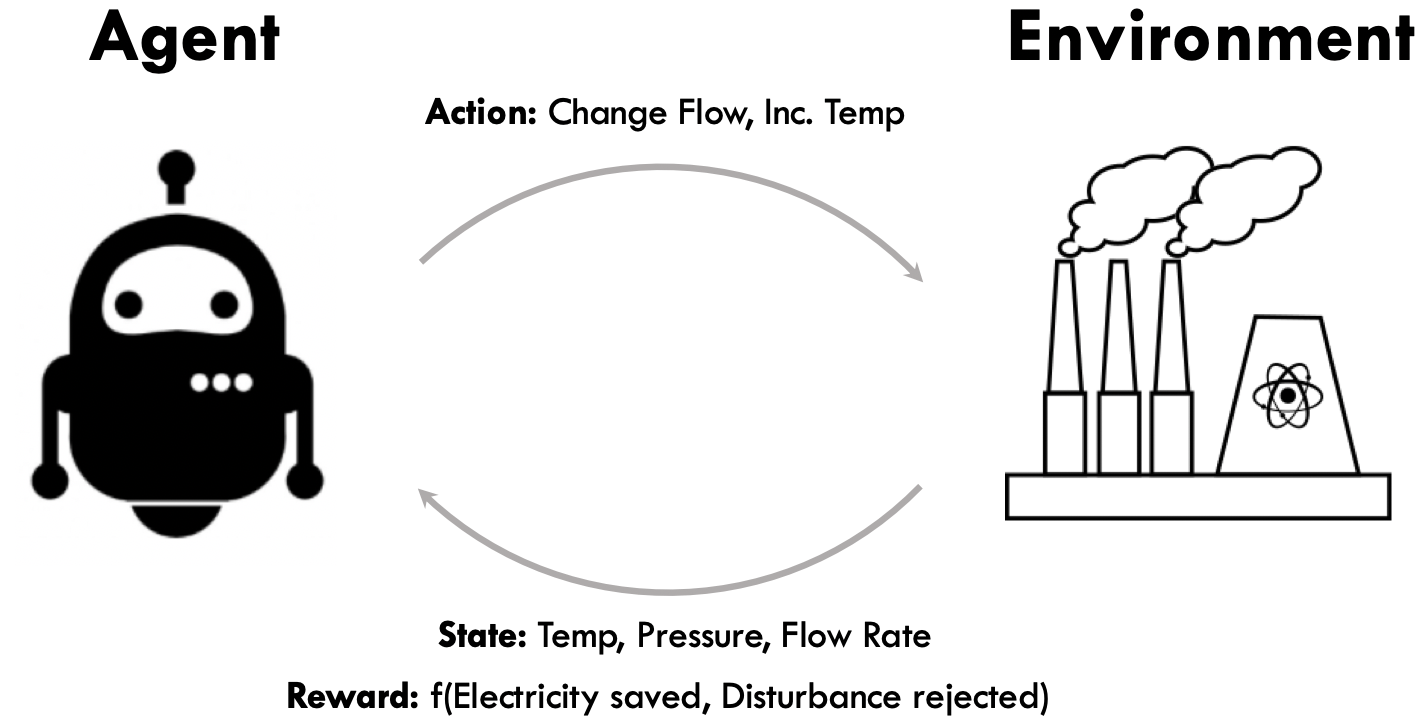
\includegraphics[scale=0.5]{images/RL.png}
    \caption{Basic setup of reinforcement learning where an agent interacts with the environment}
    \label{fig: simple_rl}

\end{figure}

Reinforcement learning consists of the following four elements:

\begin{itemize}
    \item Policy, $\pi$
    \item Reward, $R$
    \item Value Function, $V(s)$
    \item Model (optional), $\dot{x} = Ax + Bu$
\end{itemize}

The policy, $\pi$, of reinforcement learning is a direct mapping from $X \rightarrow U$.  To find the optimal policy, $\pi^*$, the agent is guided by an immediate scalar reward for each interaction (also called \textit{episode}). Policies resulting in higher rewards are more likely to be followed in the future, \textit{mutatis mutandis}.  However, reinforcement learning is concerned with the long term success rather than immediate pleasure. Often times, long term success require short term sacrifice.  Thus, the value function, $V^{\pi}(s)$, is used to describe the long term expected reward under each policy.  Initially, the value function for each state is initialized at zero.  After each episode, the value function will be updated to reflect the new knowledge obtained from the last episode through Equation \ref{eq: value_function}.

\begin{equation}
    \centering
    V(x_t) \leftarrow V(x_t) + \alpha [V(x_{t + 1}) - V(x_t)]
    \label{eq: value_function}
\end{equation}

In Equation \ref{eq: value_function}, $\alpha$ represents the step-size parameter.  That is, how big each update step should be.  Once convergence is achieved for $V(x_t)$, the optimal policy can be described by Equation \ref{eq: opt_policy}.  

\begin{equation}
    \centering
    \pi^*(x) = \argmax_u q_{\pi}(x, u), \; \forall x 
    \label{eq: opt_policy}
\end{equation}

Lastly, reinforcement learning \textit{can} consist of a model. Such cases are called \textit{model-based} reinforcement learning.  The model will be used for planning, and is a way for the agent to plan a control trajectory before they are experienced.  Contrarily, \textit{model-free} reinforcement learning learns \textit{explicitly} through interactions with the environment.

One key topic of reinforcement learning is: \textbf{exploration} vs. \textbf{exploitation}.  At first, the agent must explore to learn the state space, $\mathcal{X}$.  But the agent must know \textit{when} to stop exploring, and start exploiting (i.e., start taking advantage of what is known).  If the agent explores too much, lots of value is lost.  However, if the agent does not explore enough, the current policy may not be optimal and more value is lost long term.  Exploration vs. exploitation is one of the most important topics today in reinforcement learning, and the time to switch from exploration to exploitation will vary between problems.  In control theory, exploration vs. exploitation is known as the conflict between identification (or estimation) and control \cite{explorevexploitcontrol}.  

Another important distinction between different reinforcement learning algorithms is \textbf{on-policy} vs. \textbf{off-policy}.  On-policy methods select actions that maximizes reward given the current knowledge of the agent.  Subsequently, off-policy methods perform exploratory actions for a chance that the explored action offers superior returns to the current best known action.

In the next sub-sections, the three fundamental reinforcement learning methods (Dynamic Programming, Monte Carlo, Temporal-Difference) will be introduced.

\subsection{Dynamic Programming Methods}
\subsubsection{Value-Iteration}
\subsubsection{Policy-Iteration}
\subsection{Monte Carlo Methods}
\subsection{Temporal-Difference Methods}
\subsection{Reinforcement Learning vs. Other "Learnings"}

Machine learning consists of the following four classes: i) Supervised learning, ii) Unsupervised learning, iii) Semi-supervised learning, iv) Reinforcement learning.  Supervised learning is fitting a model to map input data to output data.  The model is initially trained on a set of labeled training data provided by a subject matter expert.  Subsequently, unsupervised learning is used on unlabeled data sets.  The objective of unsupervised learning is to explore the data and identify hidden features. Semi-supervised learning combines the strengths of supervised and unsupervised learning, and is especially useful \cite{machine_learning}.  Often times, industrial data will be partially labelled due to the time and cost associated with data labelling.  For supervised and unsupervised learning, only the labeled and unlabeled data can be used, respectively.  However, all data can be used in semi-supervised learning which allows for maximized data efficiency and increased model performance. Finally, reinforcement learning is a goal-directed learning from interactions with the environment \cite{sutton}.

Reinforcement learning is a unique class of machine learning.  An ideal supervised learning model can only be as good as the subject matter expert providing the labels to the data set, which may not be 100\%.  For example, in a complex control task, the control law is usually highly non-linear. Control experts can try to provide control strategies for such systems, but optimality may not be guaranteed for highly non-linear systems. Also, supervised learning is used to generalize responses for occurrences not present in the data \cite{sutton}.  Reinforcement learning works by directly interacting with the environment \textit{without labels}. Through adequate exploration, reinforcement learning will identify peculiar features to optimally control such problems [citation required].  Reinforcement learning is \textit{similar} to unsupervised learning in terms of identifying hidden structures within the environment.  However, reinforcement learning tries to maximize an internal scalar "reward" signal, rather than purely data mining.

Evolutionary methods, a family of optimization algorithms such as genetic algorithm, are most similar to reinforcement learning.  For a control problem, such methods can apply multiple static policies for different operating regimes \cite{sutton}.  Policy search is conducted by first initiating $k$ random input trajectories of length $N$, generating input matrix $\mathbb{U}_{[k, N]} \in \pi$.  Subsequently, the loss, $J_U$, of each $U$ is calculated based on the objective function.  Input trajectories with the lowest loss move onto the next generation and generates new pseudo-random input trajectories.  This process is repeated until optimal policy, $\pi^*$ is found for each operating regime \cite{ga_for_control}.

Evolutionary methods work well when the policy space is sufficiently small, easy to find, or a lot of time is available for optimization.  The biggest advantage of such methods compared to reinforcement learning is that the whole state does not need to be known.  However, such methods does not capture the reinforcement learning fundamentals of mapping $X \rightarrow U$.  Unlike evolutionary methods, reinforcement learning keeps memory of each indvidual interaction making it a more data efficient approach \cite{sutton}.

%%%%%%%%%%%%%%%%%%%%%%%%%%%%% End Section Intro to RL %%%%%%%%%%%%%%%%%%%%%%%%%%%%%%%%%%%%%%%


%%%%%%%%%%%%%%%%%%%%%%%%%%%%% Begin Section Tabular RL %%%%%%%%%%%%%%%%%%%%%%%%%%%%%%%%%%%%%%

\section{Tabular Q-learning}
\subsection{Introduction to Q-learning}
\subsubsection{Adaptation to Non-Stationary Problems}
\subsubsection{Incremental Implementation}
\subsubsection{Action Selection}
\subsubsection{Exploration in Tabular Q-learning}
\subsubsection{Reward Functions}
\subsubsection{Expected Returns for Different MDPs}

\subsection{Overall Setup}

%%%%%%%%%%%%%%%%%%%%%%%%%%%%% End Section Tabular RL %%%%%%%%%%%%%%%%%%%%%%%%%%%%%%%%%%%%%%%

%%%%%%%%%%%%%%%%%%%%%%% Begin Section Function Approximation %%%%%%%%%%%%%%%%%%%%%%%%%%%%%%%

\section{Function Approximation}
\subsection{Introduction to Function Approximations}
- capture the data of large data set and condense it down into something smaller.
\subsection{Neural Network Basics}
\subsubsection{Neural Network Initialization}
\subsubsection{Gradient Descent Updating}
\subsubsection{Mini-batch Gradient Descent}
\subsubsection{Batch Normalization}
\subsubsection{Regularizations}

%%%%%%%%%%%%%%%%%%%%%%%%% End Section Function Approximation %%%%%%%%%%%%%%%%%%%%%%%%%%%%%%%


%%%%%%%%%%%%%%%%%%%%%%%%%%%%%%%%% Begin Section DDPG %%%%%%%%%%%%%%%%%%%%%%%%%%%%%%%%%%%%%%%

\section{Deep Deterministic Policy Gradient}
\subsection{Actor-Critic Intuition}
\subsection{Actor - Deterministic Policy Gradient}
\subsection{Critic - Deep Q-learning}

\newpage

\subsection{Exploration in DDPG}
\subsubsection{White Exploratory Noise}
\subsubsection{Ornstein-Uhlenbeck Exploratory Noise}
\subsection{Stabilization of Training}
\subsubsection{Experience Replay}
\subsubsection{Target Network}
\subsubsection{Adaptive Batch Gradient Descent}
\subsubsection{Reward Clipping}
\subsection{Input and State Constraints}
\subsection{Training Algorithm}

%%%%%%%%%%%%%%%%%%%%%%%%%%%%%%%%%% End Section DDPG %%%%%%%%%%%%%%%%%%%%%%%%%%%%%%%%%%%%%%%%



\section{Previous RL applications in process control}

%%%%%%%%%%%%%%%%%%%%%%%%%%%%%%%%%%%%%%%%%%%%%%%%%%%%%%%%%%%%%%%%%%%%%%%%%%%%%%%%%%%%%
% Model Predictive Control
%%%%%%%%%%%%%%%%%%%%%%%%%%%%%%%%%%%%%%%%%%%%%%%%%%%%%%%%%%%%%%%%%%%%%%%%%%%%%%%%%%%

%%%%%%%%%%%%%%%%%%%%%%%%%%%%%%%%%%%%%%%%%%%%%%%%%%%%%%%%%%%%%%%%%%%%%%%%%%%%%%%%%%%%%
% Model Predictive Control
%
%
%
%
%%%%%%%%%%%%%%%%%%%%%%%%%%%%%%%%%%%%%%%%%%%%%%%%%%%%%%%%%%%%%%%%%%%%%%%%%%%%%%%%%%%

\section{Model Predictive Control}

Compared to all topics in process control, the concepts of model predictive control (MPC) is perhaps the closest resemblance to modern RL.  MPC is a model-based control strategy (known as a planning method in RL literature) that optimizes the input trajectory of a system by using the functional equation (a function where the unknowns are also functions) generated from the system's state information together with a value function. The performance of MPCs heavily rely on the accuracy of system identification as the input trajectory is solved by extremizing an objective function using mathematical programming (MP) as a function of the process model \cite{mpc}. The objective function is typically given as:
\begin{equation}
    J = \sum\limits^{N}_{i = 1} x_i^TQx_i + \sum\limits^N_{i=1}u_i^TRu_i
    \label{eq:mpc_cost}
\end{equation}
where $N$, $Q$, and $R$ are the prediction horizon and tuning matrices, respectively. Superscript $T$ denotes the transpose operation. $Q$ and $R$ are diagonal matrices and are used to emphasize importance on different state and inputs, respectively. Here, $x$ and $u$ are given as:
\begin{equation}
    x_{sp} - x_i
\end{equation}
\begin{equation}
    u_{ss} - u_i
\end{equation}
where subscripts $sp$ and $ss$ denote the set-point and steady state, respectively. Often times in optimal control, $u_{ss}$ is unknown. In such scenarios, $u$ is given as $\Delta u$ instead, representing a cost in changing the inputs at each step.

Implementation-wise, MPC uses a receding horizon approach where the controller predicts and optimizes for a set amount of steps into the future.  However, only the first control action is implemented.  During the next sampling time, the trajectory is re-optimized and the cycle repeats. The length of the input trajectory and the number of steps the controller predicts into the future are known as the control and prediction horizon, respectively. During design, it is paramount to ensure that both the prediction and control horizons are adequate in length to ensure global optimal solutions.  Intuitively, the prediction and control horizon can be related to the everyday task of driving a car.  It would be very dangerous if we only consider events one second into the future because it would be difficult to react to curves and other road side disturbances; therefore, the prediction and control horizons must be sufficiently long to ensure safe and optimal driving practices. Typically, the control horizon is chosen to be shorter than the prediction horizon due to computational cost and the unimportance of unnecessarily long input trajectories \cite{prediction_horizon}.  One flaw with the receding horizon approach is its extremely expensive online computational cost, especially in large non-linear systems.  

Explicit MPC was developed to mitigate this computational burden by leveraging parametric programming to pre-compute solutions to the optimization problem offline \cite{explicit_MPC}.  During online evaluation, the controller simply looks up the optimal input from a dictionary of pre-computed solutions, making online evaluation extremely fast. This idea is exactly equivalent to RL, where the agent is trained offline (i.e., solves the optimal policies offline), allowing extremely fast online evaluations. 

Ultimately, MPCs provide many advantages compared to classical control strategies.  For example, MPC considers long term planning and identifies the optimal input trajectory rather than the best immediate action.  Furthermore, MPCs have predictive capabilities and can anticipate future events, allowing the controller to plan future control actions accordingly.  A third advantage is that the MP methods used in MPC have been widely demonstrated to handle both input and state constraints relatively successfully.  In modern times, MPCs are often implemented in the supervisory control layer.

The process control hierarchy is shown in Figure \ref{fig:rto_mpc_pid}. Starting from the bottom, the \textit{regulatory controllers} are typically used to ensure stability of the process and directly actuate the process instrumentation.  A common regulatory controller is the Proportional-Integral-Derivative controller (PID). The layers above are known as the \textit{supervisory controllers}. MPC is a common supervisory controller and is classically implemented for regulation or set-point tracking problems exclusively.  Economic objectives of the process were managed by the real time optimization (RTO) layer through steady state optimization \cite{rto}. More recently, control practitioners began to unify the ideas of RTO and MPC into a centralized algorithm called economic model predictive control (EMPC).  Here, the economic objective of the RTO is placed into the objective function of the MPC, allowing for the input trajectory to optimize the economic objective instead \cite{empc2, empc1}. 

\begin{figure}[H]
    \centering
    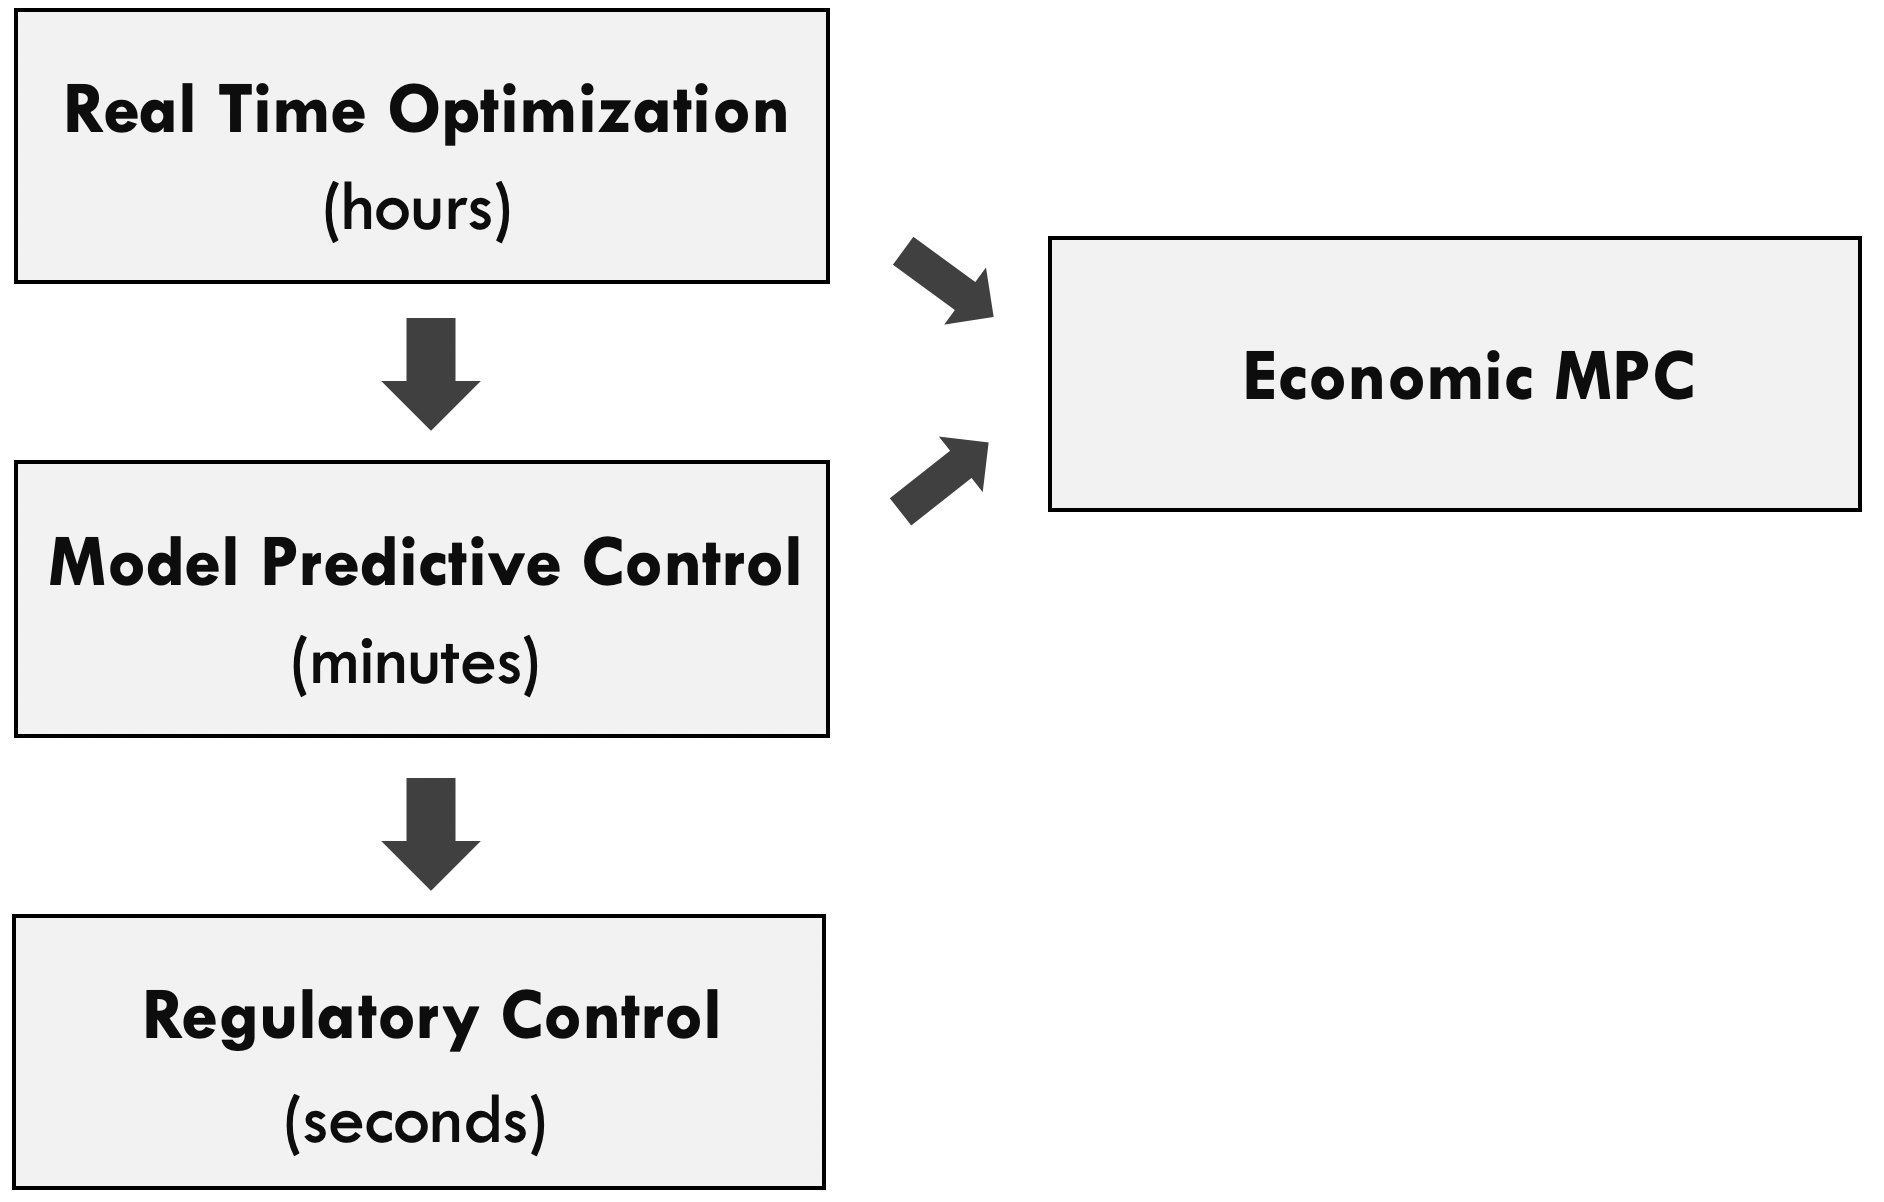
\includegraphics[width=0.5\textwidth]{images/ch1/rto_mpc_pid.jpeg}
    \caption{The traditional control architecture.}
    \label{fig:rto_mpc_pid}
\end{figure}

Comparatively, RL can be described as a general control algorithm and can be used to replace \textit{any} layer in Figure \ref{fig:rto_mpc_pid}. For example, a MPC or PID based RL would have its reward function to be identical as the negative of Equation \ref{eq:mpc_cost}.  In the EMPC case, the reward function of RL would instead be the economic objective.  In Chapter 4, the performance of RL based supervisory controls will be extensively compared to traditional methods on simple and complicated processes. Additionally, the pros and cons of each method will be summarized.


% \chapter{Machine Learning for Prediction Applications}
% %%%%%%%%%%%%%%%%%%%%%%%%%%%%%%%%%%%%%%%%%%%%%%%%%%%%%%%%%%%%%%%%%%%%%%%%%%%%%%%%%%%%%
% Machine Learning in Prediction
%
% 1. Linear Models
% 2. Polynomial Models
% 3. Neural Networks
% 4. Linear parameter-varying models
% 5. Adaptive nature using ISIS algorithm
% 
%%%%%%%%%%%%%%%%%%%%%%%%%%%%%%%%%%%%%%%%%%%%%%%%%%%%%%%%%%%%%%%%%%%%%%%%%%%%%%%%%%%

Cheap data storage and escalation of computational power allowed the world to enter a new age: the age of \textit{big data}. With vast amounts of data, previously in-viable and data hungry machine learning algorithms are now implementable.  The technology sector was the first group to be able to exploit this arcane technology to create tremendous value in applications ranging from targeted advertisements to self driving cars. The value was so great that the current top four companies in America by market capitalization are all technology companies (Microsoft, Apple, Amazon, and Facebook) as of 2019. As the technology sector's successes grow, other industries begin to catch a glimpse of the potential value creation in their own respective industries and initiate their own digital revolution. The ripples of success from the technology industry ultimately resulted in waves of capital investments into machine learning (ML) and artificial intelligence (AI) from all industries.

ML solutions promise to be cheaper, more accurate, and have online learning abilities compared to traditional methods.  Additionally, the solutions are promised to be easier to implement and will take less time to design; feed it data and it will learn, as they claim.  With this mentality, machine learning engineers and data scientists from technology companies attempted to conquer other industries, one industry being process control and chemical engineering. Unfortunately, their crusade fell short and their successes were few due to their lack of engineering knowledge and inability to identify large value gains.  Typically, projects in technology companies deal with very unambiguous information such as identifying location of objects or predicting the enjoyments of an individual based on previous articles they have read. However, process control typically generate time-series data and are often very ambiguous with data characteristics unique to the industry. Some characteristics include time delayed data, multi-modal data, unreliable data, highly noisy data, state transition dynamics data, and any combination of the prior.  Due to the increased complexity, data pre-processing for ML projects in the process control industry is mission critical and much more vigorous for successful applications.

Table \ref{tab:2MLApplications} shows some general machine learning applications for the process control industry. Currently, ML applications in the process industry can be broken down into prediction, monitoring, and control.  The field of prediction deals with mapping from certain inputs to desired outputs. An example would be building a soft sensor to predict for a state, $x_{m}$, that is expensive to measure.  By identifying states highly correlated to $x_{m}$, a multivariate soft sensor can be built to inexpensively predict the state in the future. In ML monitoring, the algorithms are tasked to monitor the process for anomalous activities. Here, an example would be applying a classification method to predict for failures in process equipment.  Lastly, ML control is concerned with the topics of adaptive, multivariate optimal control. Reinforcement learning is the typical ML algorithm for control.  

\begin{table}[h]
    \centering
    {\setstretch{1.2}
    \begin{tabular}{c|c|c}
    Prediction & Monitoring & Control \\ \hline
    Soft sensing & Anomaly detection & Supervisory control \\
    Forecasting  & Anomaly prediction & Regulatory control \\
    Operator education  & Alarm prioritization & Operator education \\
    Digital twin  & Alarm reduction & Multivariate control\\
    \end{tabular}}
    \caption{General applications for machine learning in the process control industry.}
    \label{tab:2MLApplications}
\end{table}

 Figure \ref{fig:02AICloud} shows a the machine learning architecture that is generic enough for implementation in all industrial plants. First, the industrial process (e.g. refinery, pipeline, reactor, etc.) sends raw sensor data into the cloud, where it is cleansed through data pre-processing methods.  Then, the filtered data is sent into different machine learning algorithms depending on the objective of the application and will output the desired values.  After a set time frame, all ML models will then be re-updated to learn the newest experiences. For computations requiring speedy outputs, portions of the ML code can also be pushed to the local devices using Microsoft Azure IoT edge devices. 

\begin{figure}[h]
    \centering
    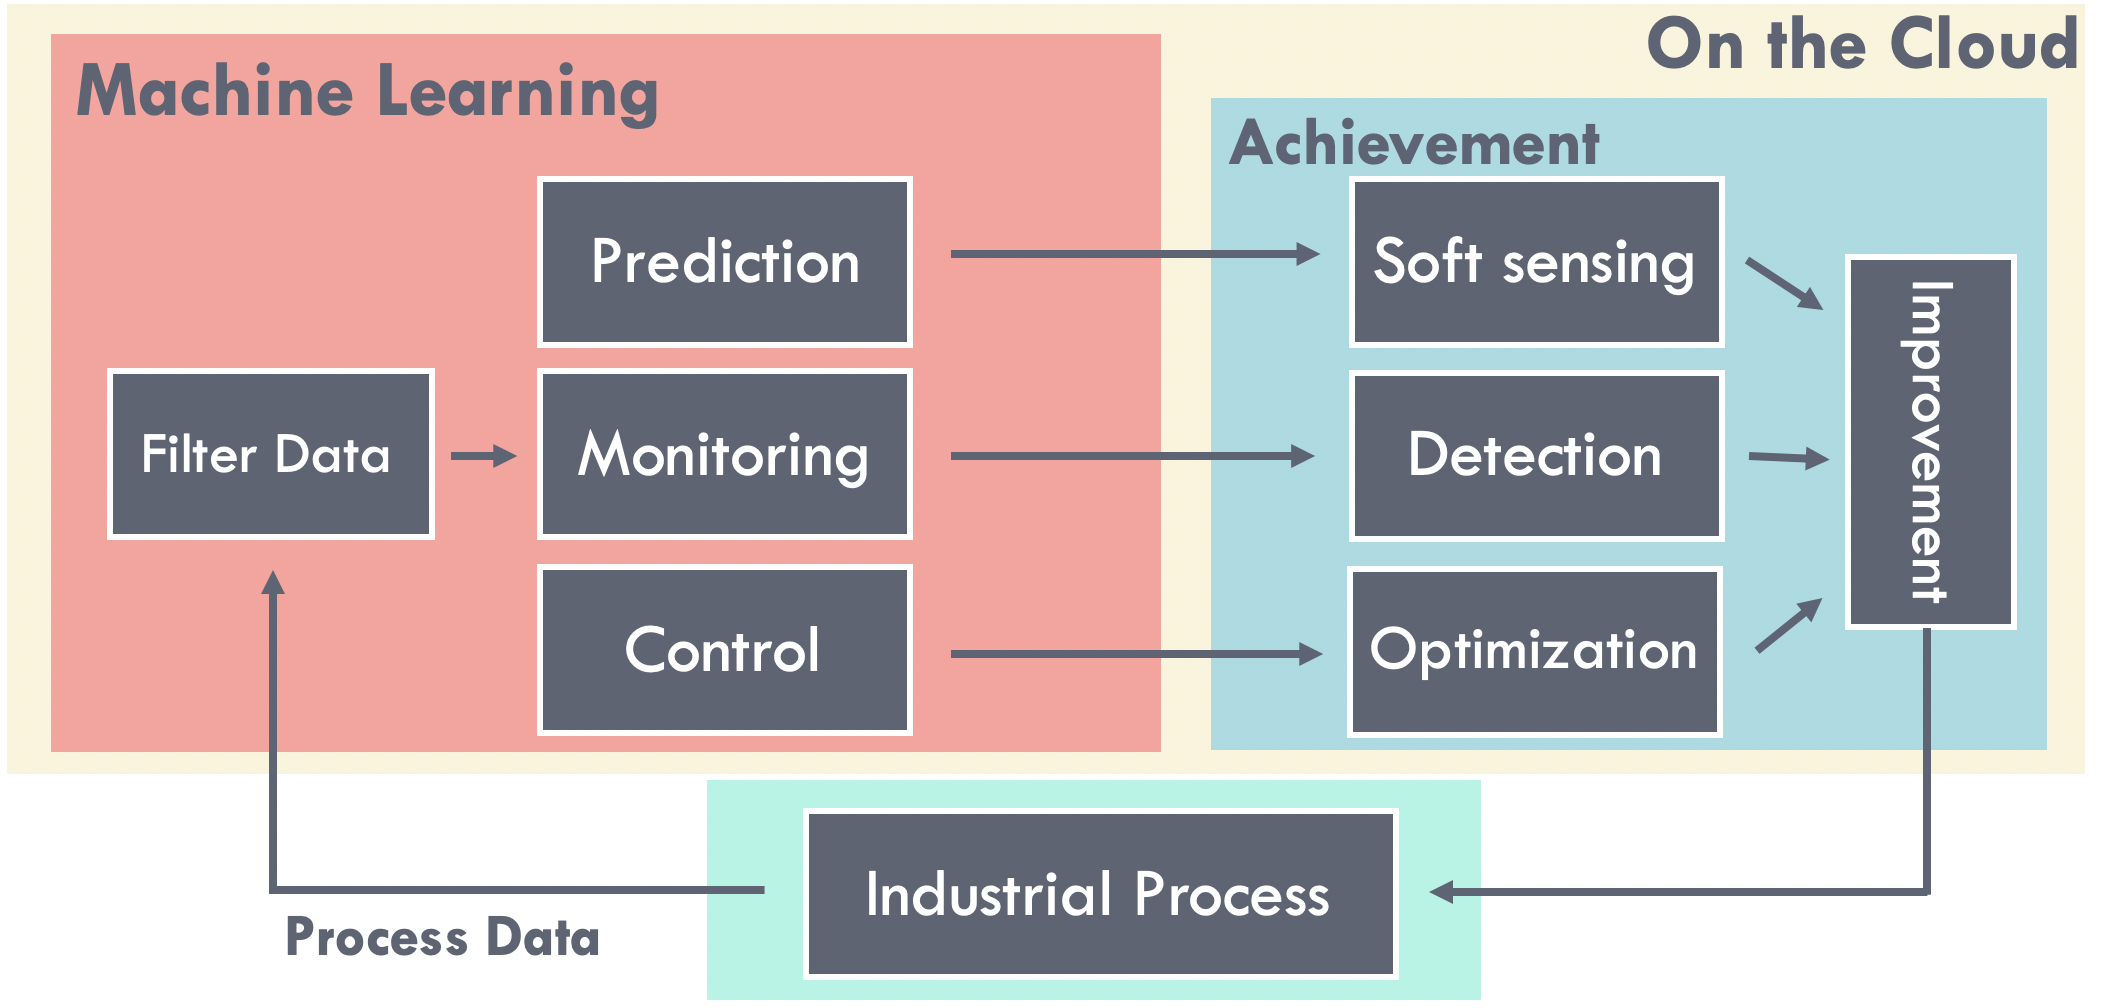
\includegraphics[width=\textwidth]{images/ch2/02AICloud.png}
    \caption{Overall machine learning architecture in an industrial environment}
    \label{fig:02AICloud}
\end{figure}

The objective of this chapter was to convey ideas for implementing machine learning solutions catered towards the \textbf{process control} industry.  In this chapter, the first half consists of common data pre-processing techniques to handle common process control concerns and is visually described by the "Filter Data" box.  The second half contains machine learning methods (in order of difficulty) to handle different process control prediction problems ("Prediction" box in the above figure). To conclude this chapter, the prediction algorithms will be closed off with an adaptive modelling technique inspired by reinforcement learning and adaptive resonance theory. For validation purposes, the machine learning methods were implemented onto an industrial pipeline for prediction, monitoring, and optimization\footnote{This project was supported in part by Mitacs through the Mitacs Accelerate program.}\footnote{This chapter only contains the theory and application highlights. The detailed industrial project report can be found in Appendix A.}.

Contributions made in this chapter include:
\begin{enumerate}
    \item Effective data pre-processing techniques for the process industry
    \item Catering machine learning prediction techniques to the process industry
    \item An outlier-free, data efficient, adaptive modelling method for multi-modal operations
\end{enumerate}

\section{Data Pre-processing}
Data pre-processing typically includes many steps starting with filtering by subject matter expertise, and then transitioning to common statistical methods.  For this section, only the filtering methods unique to process control will be discussed. Please refer to Appendix A for details regarding the other steps. Process control is typically concerned with multivariate time-series data plagued with noisy and/or unreliable sensor readings. Time delays are critical to successful prediction applications in process control. Furthermore, some processes may also have a variety of different operating regimes depending on downstream demand or ambient conditions.  In order to have successful prediction algorithms for process control, all of the above must be considered.

\subsection{Time Delay Data}
Time delay is the time between the performance of a control action and the change in output. Time delays occur due to the physics of the natural world.  For example, turning on a pump at the beginning of a pipeline does not result in higher flow rates immediately.  The process takes time to adjust and \textbf{transition} to the new steady state; therefore, raw data must be first shifted to account for the time delay.  Without doing so, models would be using current information to predict the past.  Imagine building a model to predict for the outlet flow rate of a pipeline where the regressors are pump statuses 300 km upstream of the outlet.  If a change in pump status occurred at $t = 0$, the pressure will take a few minutes to propagate down the pipeline.  Thus, the model taking pump statuses at $t = 0$ must have its flow rate labels shifted from $t = \tau$, where $\tau$ is the expected time delay.  An example of the time delay shifting procedure for an industrial pipeline is shown in Table \ref{tab:08TimeToCC} located in Appendix A, where data was shifted for different locations along the pipeline to enhance predictive capabilities.

Initial engineering expertise and/or data analysis must be conducted to identify the time delay for specific processes.  For example, it is well known that pressure propagates down incompressible fluids at approximately the speed of sound (1480 km/h) \cite{fluid_mechanics}.  Using this information, adjusting for the time delays along the pipeline was made trivial.

\subsection{Multi-modal Data}
In the process industry, it is common to have multiple modes of operation due to changing ambient conditions (e.g. summer, winter), different market demands, and a variety of other factors.  Each operating condition also consists of unique equipment operation and process characteristics (flow rates, temperatures, etc.); therefore, a common model to predict for many different operating conditions lead to increased model errors.  Here, unsupervised learning should be used to avoid this scenario for systems with many modes.  More specifically, clustering methods should be applied to segregate data from different operating modes, and separate models should be built using data from each operating mode to enhance accuracy.  For big data applications, \textit{k}-means or density based scanning (DBSCAN) should be used due to their scalability and non-iterative nature \cite{clustering_complexity}. Of the two methods, \textit{k}-means is much faster while DBSCAN is more robust to outliers.

An example of the breakdown of a multi-modal system can be found in Figure \ref{fig:08DBSCAN} in Appendix A.  By segregating the system into multiple modes, more accurate weights can be identified for each mode compared to general weights for all modes.  In fact, most modes would not even use the same equipment.  Such a concept is similar to using a linear parameter-varying model to approximate a non-linear system.  

\subsection{Unreliable and Noisy Data}
Thousands of measured data are recorded per minute on modern distributed control systems. However, many process variables such as viscosity, or parts per million (ppm) are difficult to measure with modern equipment on a live process. This results in inaccurate values being sent to the ML models, ultimately reducing accuracy.  To overcome highly unreliable data, a general strategy is to identify how the operator(s) are using the data and to engineer the feature(s) to be used in the same way for the ML model.  For example, the densitometers installed along the industrial pipeline shown in Appendix A all show different readings for the same crude. At times, the reading could be off by $\pm 20\%$. However, the operators only use the density reading to determine the grade of crude inside the batching pipeline. The crude is light if the API is above a threshold, heavy otherwise.  The physical number had no meaning for them.  To improve the ML model accuracy, the density reading was feature engineered to be a binary variable reading "1" if the API was above the threshold, "0" otherwise.  By doing so, the variable in the ML model was used in the same way as the operators and the accuracy increased.

Other data measurements may be accurate, but highly noisy. Noisy measurements may lead to significant predictive errors 
Noise can be reduced significantly by applying an exponentially weighted moving average (EWMA) filter given by:
\begin{equation}
    v_t = \beta v_{t - 1} + (1 - \beta) \theta_t, \; v_0 = 0
    \label{eq:08EWMA}
\end{equation}
\begin{equation}
    v_t \leftarrow \frac{v_t}{1 - \beta^t}, \forall v \in V
    \label{eq:08Bias_Correction}
\end{equation}
where $v_{t}$ is the exponentially weighted value at time $t$.  $\beta$ is the exponentially weighing factor.  Larger $\beta$ results in smoother results.  $\theta_t$ is the original value at time $t$. $V$ is a vector representing the exponentially weighted values before bias correction. EWMA is a very effective way to remove noise in chemical processes because these processes typically contain slow dynamics. By exponentially smoothing the data, the fast peaks are removed while preserving the slow dynamics. An example of the EWMA algorithm applied to the measurement of drag reducing agent (DRA) ppm values is shown in Figure \ref{fig:08DRA} in Appendix A.  DRA ppm measurements are known to be highly noisy; however, the noise can be almost completely removed by applying EWMA.

\subsection{State Transition Dynamics}
Another unique topic of process control is the dynamics of the system. System dynamics refer to the transitional period of going from one steady state to another after a control input is provided. Typically, dynamical models are used for advanced process controls where optimizing for the dynamics of the system is critical for optimal performance.  In order to build machine learning models to describe the dynamics of systems, a time-series implementation must be pursued.  Typical ML models map states and control actions at time $t$ to the desired output at time $t_{ss}$, where $t_{ss}$ is the time required for the system to transition to the new steady state.  By doing so, the dynamics of the system are completely omitted.  In order to build a dynamical ML model, the raw data needs to skip the time delay pre-processing step and be augmented by time.  Imagine a simple single-input single-output (SISO) system:
\begin{equation}
    y = w_1x + b
\end{equation}
In time-series implementation, the model would instead be:
\begin{equation}
    y_{t + 1} = w_1x_{t} + w_2x_{t - 1} + w_3x_{t - 2} + ... + y_{t} + y_{t - 1} + ... + b
    \label{eq:02_1step}
\end{equation}
where the input vector would be augmented as $\mathcal{X} = [x_{t} | x_{t - 1} | x_{t - 2} | ... ]$. Here, Equation \ref{eq:02_1step} becomes the 1-step ahead predictor of the system and dynamics can be predicted for. This data augmentation method is identical to all ML models if a time-series implementation is desired. In Appendix A, Figure \ref{fig:08ts_ls} shows an example of a time-series prediction model.  Because such models only predict one step in advance, error is typically very low.  The predicted value can also be fed in recursively to generate a infinite step ahead prediction that can be used for forecasting long term trends.

\section{Machine Learning Methods}

Many ML methods exist for prediction, each having its advantages and disadvantages. In this section, the most common ML methods will be shown along with their applications in process control.  Unique hyper parameters for different ML methods will also be shown; however, common hyper parameters such as $\alpha$, training epoch, and mini-batch size are common throughout and will be omitted.  Furthermore, common model performance metrics will be introduced. 

\subsubsection{Performance Assessment}
The model performance were assessed using the following three ways:
\begin{enumerate}
    \item Root mean squared error (RMSE) \cite{NN}:
    \begin{equation}
        J = \sqrt{\frac{1}{n}\sum\limits^n_{i=1}(\hat{y}_i - y_i)^2}
        \label{eq:08RMSE}
    \end{equation}
    
    \item Mean absolute error (MAE) \cite{NN}:
    \begin{equation}
        J = \frac{1}{n}\sum\limits^n_{i=1}|\hat{y}_i - y_i|
        \label{eq:08MSE_Error}
    \end{equation}
    \item Coefficient of determination ($R^2$) \cite{NN}:
    \begin{equation}
        R^2 = 1 - \frac{\sum\limits^n_{i = 1}(\hat{y_i} - y_i)^2}{\sum\limits^n_{i = 1}(y_i - \bar{y_i})^2}
    \end{equation}
\end{enumerate}
Table \ref{tab:02performanceassessment} shows the advantages and disadvantages of each assessment metric.
\begin{table}[h]
    \centering
    {\setstretch{1.2}
    \begin{tabular}{ c | p{6.2cm} | p{6.0cm}}
         Method             & Advantages        &  Disadvantages \\
        \hline
        RMSE                &  Useful for identifying large errors                            &  Smaller errors are muted        \\
        
        MAE                 &  Easy to interpret as all errors have the same weight           &  Inferior to RMSE when large errors are undesirable \\
        
        $R^2$               &  Easy to understand, {\small $-\infty \leq R^2 \leq 1$   }                                      &  Valid only for linear relationships       \\             
    \end{tabular}}
    \caption{Pros and cons of different model performance assessment methods.}
    \label{tab:02performanceassessment}
\end{table}


\subsection{Linear Models}
Linear models have two variants, linear regression and logistic regression.  The former is used for prediction tasks associated with continuous variables while the latter is used for classification tasks.  For example, linear regression is a great algorithm for soft sensor applications whereas logistic regression is more suitable for monitoring for anomalous activities. In this chapter, only the prediction variant will be shown. The model structure of linear regression is given as:
\begin{equation}
    \hat{y} = W_1^Tx + W_2^Tu + b
    \label{eq:02LS}
\end{equation}
where $x \in R^n$ is a vector of states, $u \in R^{m}$ is a vector of inputs and superscript $T$ denotes the transpose operation.  $\hat{y}$ is the predicted variable and can be anything; in soft sensors, $\hat{y}$ would be the "soft sensed" variable.  

The most common model structure for ML in the process control industry are linear models despite all processes being non-linear.  This is because the narrow region most processes operate around can typically be assumed to be linear \cite{process_control_ref13}.  Additionally, linear models are simple, interpretable, and require low amounts of data. However, the draw backs of linear models are their poor performance in the big data era where large amounts of data is available (see Figure \ref{fig:02learning_aggro}).  This trait is intensified given high dimensional data sets where identifying interaction effects are critical for accurate predictions.

Linear models were applied to the industrial pipeline as a benchmark algorithm.  The performance of the linear models can be seen in Tables \ref{tab:08LSperformance}, \ref{tab:08ConstLSPerformance} and Figures \ref{fig:08LSPlots}, and \ref{fig:08CLSPlots}. 

\begin{figure}
    \centering
    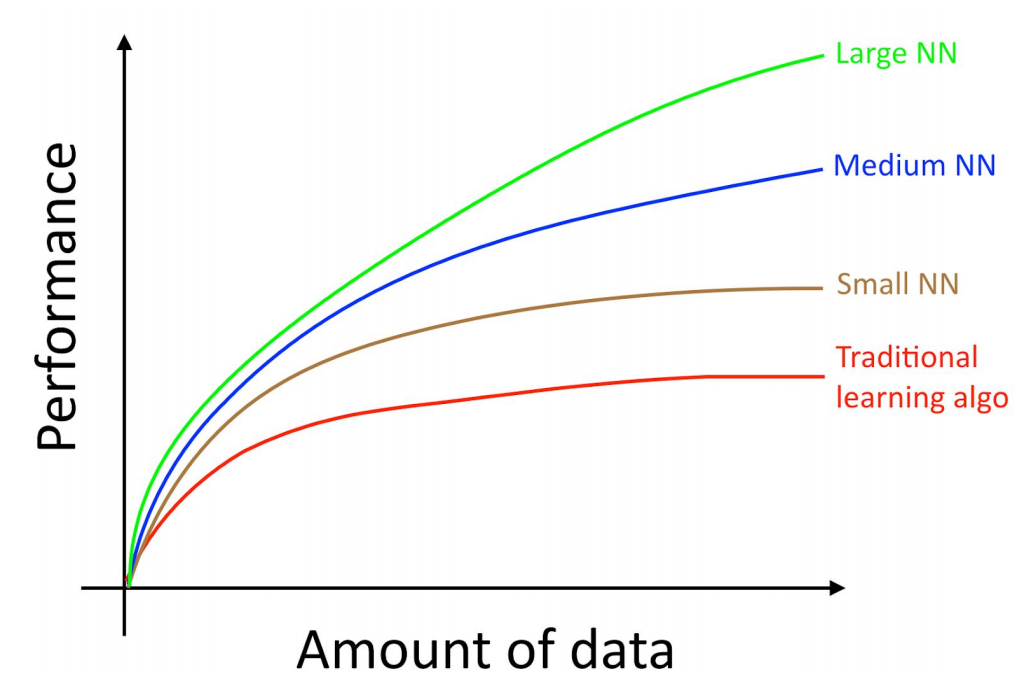
\includegraphics[width=0.7\textwidth]{images/ch2/02Learning_Aggro.png}
    \caption{Performance as a function of data.  Original image from \cite{deeplearning_course}.}
    \label{fig:02learning_aggro}
\end{figure}

\subsection{Polynomial Models}
Polynomial models are a general class of non-linear models that explores the main and interaction effects of its regressors.  The general model structure of a two regressor polynomial model is given by:
\begin{equation}
    \hat{y} = w_1x_1 + w_2x_2 + w_3x_1^2 + w_4x_2^2 + w_5x_1x_2 + e
\end{equation}
where $w$ are the weights, $x$ are the regressors, and $e$ is the modelling error.  In this model, linear, quadratic, and interaction effects are all explored simultaneously. However, the amount of parameterization required for a high dimensional prediction problem using this model structure might be difficult to interpret, thus, a truncated version of the model could be used instead for high dimensional problems. One special case of a truncated polynomial model is the exponential model given by:
\begin{equation}
    \hat{y} = w_1 x_1^{w_2} + b
\end{equation}
where the power of the regressor is also a weight to be identified. This is advantageous in situations where the non-linearity of the system is unknown. A quadratic and square root version of the exponential model were applied to the pipeline and the performances are shown in Table \ref{tab:08quad_sqrt_performance} and Figure \ref{fig:08PolynomialPlots}.  Compared to the linear models, the errors were reduced by up to 10\%.

\subsection{Neural Network and Deep Learning Approaches}
Neural network and deep learning approaches shine for predictive tasks where predictive power is the primary driver, while interpretability is not an issue, and acceptable\footnote{Neural network models are typically executed on servers and the outputs are sent to the actuators.  For fast processes, deep learning models should be pushed to the edge device.} hardware exists.  Deep learning is a special case of neural networks where many hidden layers exist.  The general consensus of the AI and ML community is that any neural network with more than three hidden layer is considered deep learning; however, the idea is not concrete and is open to personal preference.  The neural network model structure is highly non-linear and attempts to explore interaction effects of all regressors.  For a more detailed explanation on neural networks, the notation of its the variables, and its theory, please refer back to Chapter 1. Only a brief summary of the theory will be provided here. Due to the model complexity and high parameterization of neural networks, its predictive powers are unparalleled compared to other methods and can fit any function. In \cite{nn_fit}, the authors showed that:
\begin{framed}
\begin{quote}
There exists a two-layered neural network with ReLU activation functions and $2n+d$ weights that can represent any function on a sample of size $n$ in $d$ dimensions. 
\end{quote}
\end{framed}
Three distinct types of neural networks exist: i) Multilayer perceptrons (MLPs); ii) Recurrent neural networks (RNNs); iii) Convolutional neural networks (CNNs).

A visual representation of a MLP is shown in Figure \ref{fig:02MLP}.  MLPs (also known as feedforward neural networks) are the simplest and most common of the three.  In MLPs, the outputs of each neuron, $a_j^{[r]}$, is computed as:
\begin{equation}
    a_j^{[r]} = f(w_1x_1 + w_2x_2 + ... + w_mx_m + b)
\end{equation}
where the function, $f$, is non-linear and known as the \textit{activation function}.  The purpose of $f$ is to introduce non-linearity to the model; a critical addition because no process in the real world is linear.  In an intuitive sense, MLPs can be visualized as a brute force approach to identify the interaction effects of every regressor with each other. Due to the sheer number of parameterization, MLPs are very effective in predicting in-sample data points.  However, the models suffer tremendously during events where the testing data is significant different. Large MLPs also tend to overfit; thus, it is critical to increase regularization as the MLP increases in size.

\begin{figure}[h]
    \centering
    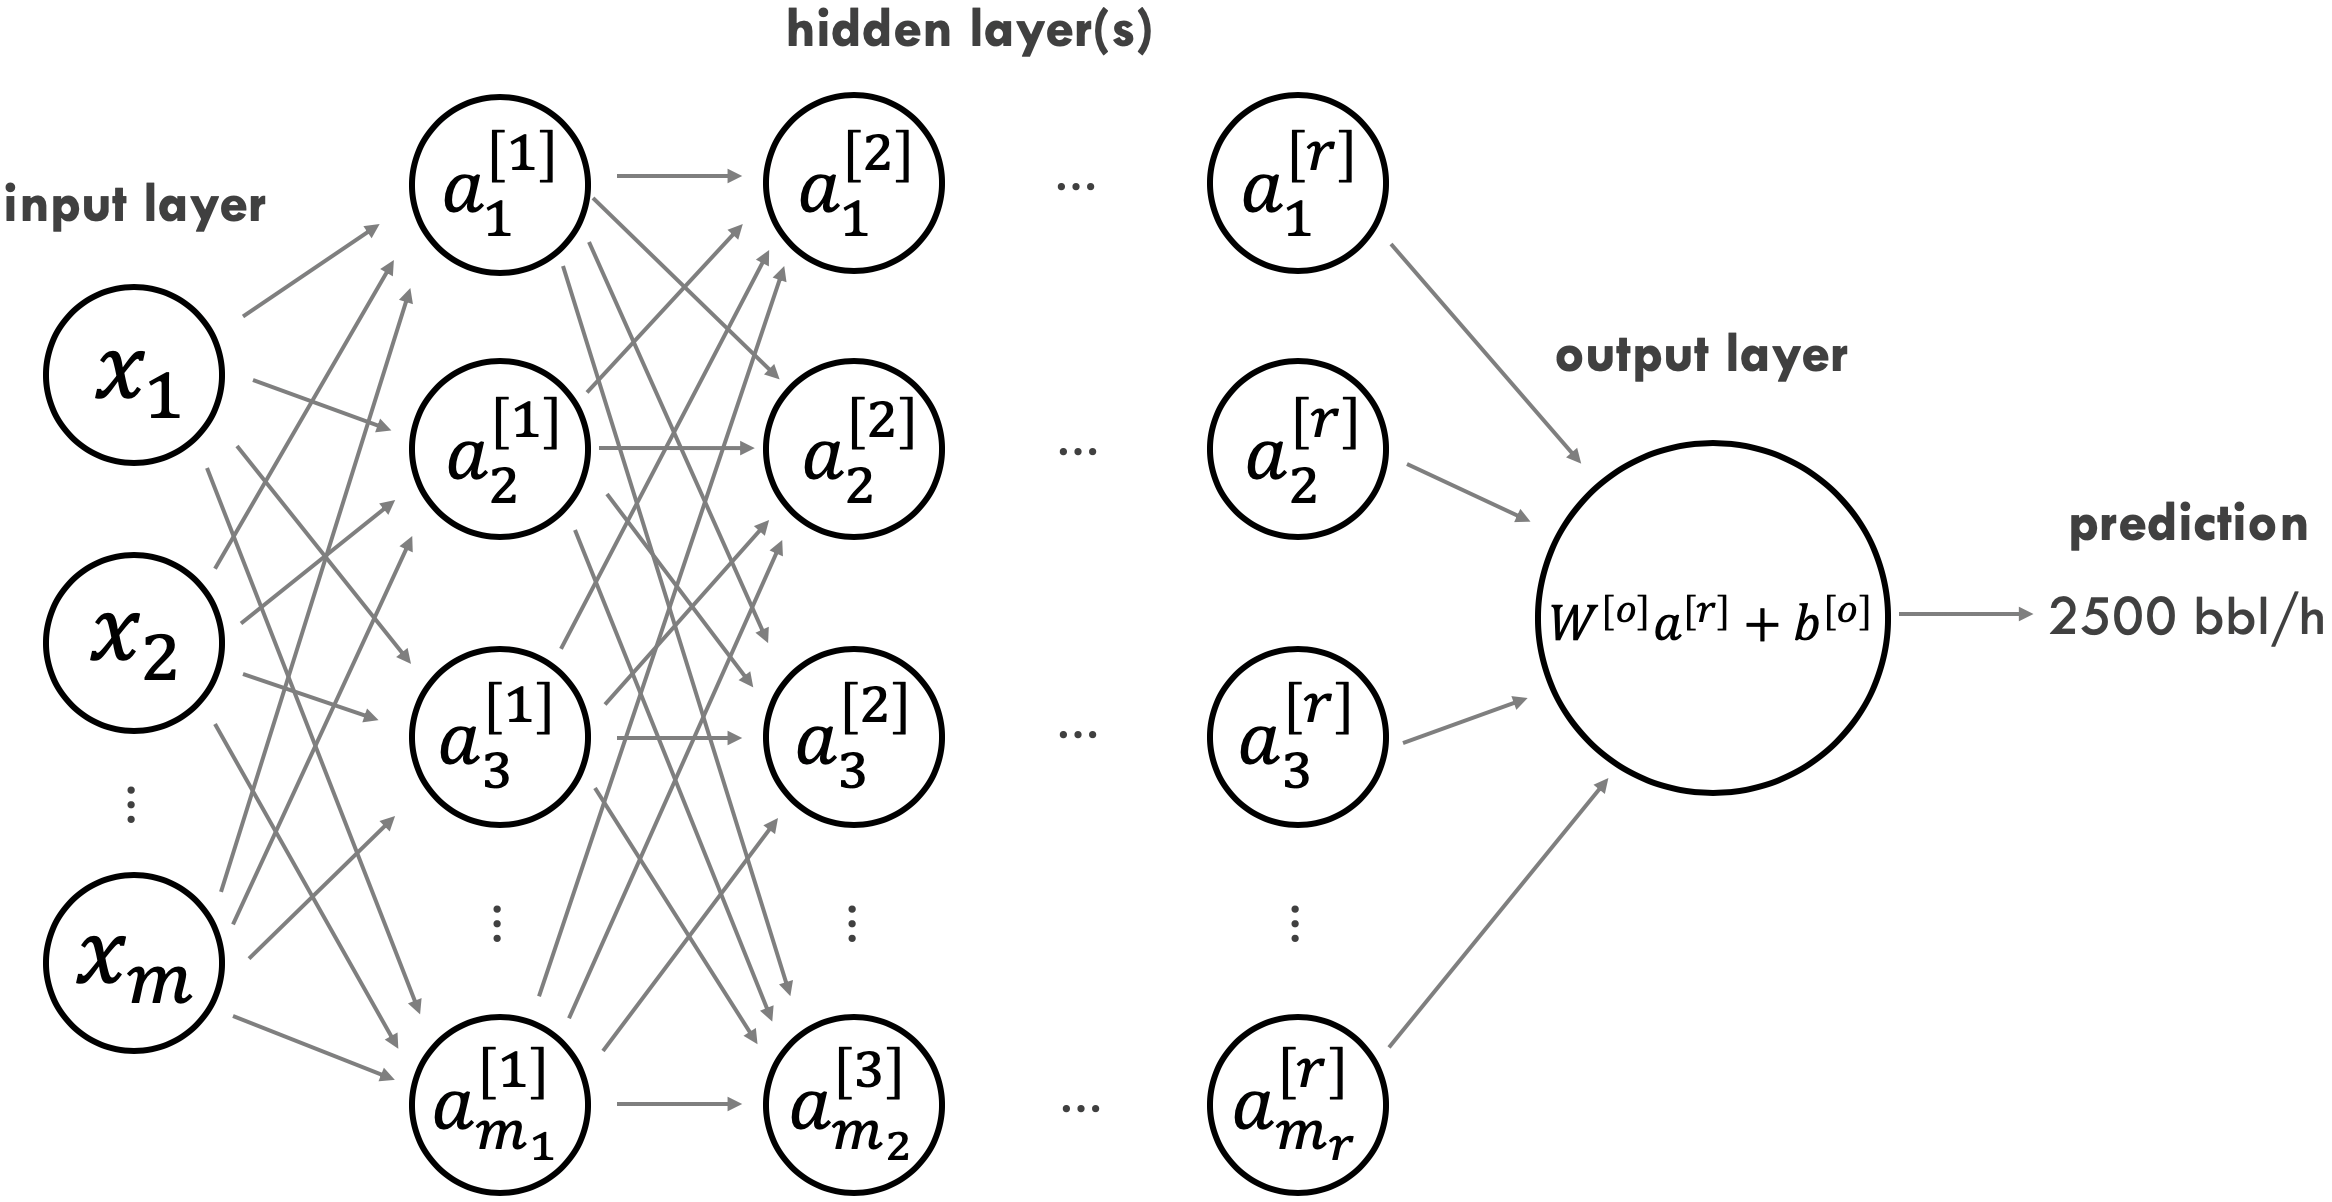
\includegraphics[width=0.9\textwidth]{images/suncor/08NN.png}
    \caption{Structure of a general neural network.}
    \label{fig:02MLP}
\end{figure}

MLPs were also applied to the industrial pipeline to model for the outlet flow rate. The input variables were measurements of variables along the pipeline such as temperatures and pressure, and the output was the outlet flow rate. Three different MLPs with varying sizes were applied.  Their respective performances can be seen in Table \ref{tab:08_nn} and Figure \ref{fig:08PolynomialPlots}.  It can be seen that the performance on the training and validation data were both excellent, though the error on the testing data increased significantly.  This was caused by the testing data being significantly different from the training data.  Data for model training was collected during the winter months, but was tested on summer months where the temperatures increased by up to $\ang{10}$ C. The increase in temperature resulted in reduced viscosity of the shipped crude and significantly hindered the predictive power of the MLPs. Ultimately, the MLPs' performance on the test data was almost identical to the much simpler polynomial models and was not used.

An especially useful type of neural networks for the process industry are RNNs (Figure \ref{fig:02RNN}) due to their time-series architecture.  Naturally, RNNs are set up to be infinite step ahead predictors and identifies temporal correlations within the data.  Traditional applications of RNNs can be found in speech recognition, translation, and language modelling.  In the process control industry where time-series data is abundant, RNN is the natural choice for typical soft sensing applications.  On a high level, RNNs accept inputs $x_t$, and outputs $y_t$.  At the same time, $y_t$ is sent as an input, along with $x_{t+1}$, back into the RNN to compute for $y_{t+1}$.  A similar computation is conducted until the end of the sequence of inputs.  By recursively re-inputting outputs as input data, RNNs are able to predict for an output trajectory given an input trajectory.

\begin{figure}[h]
    \centering
    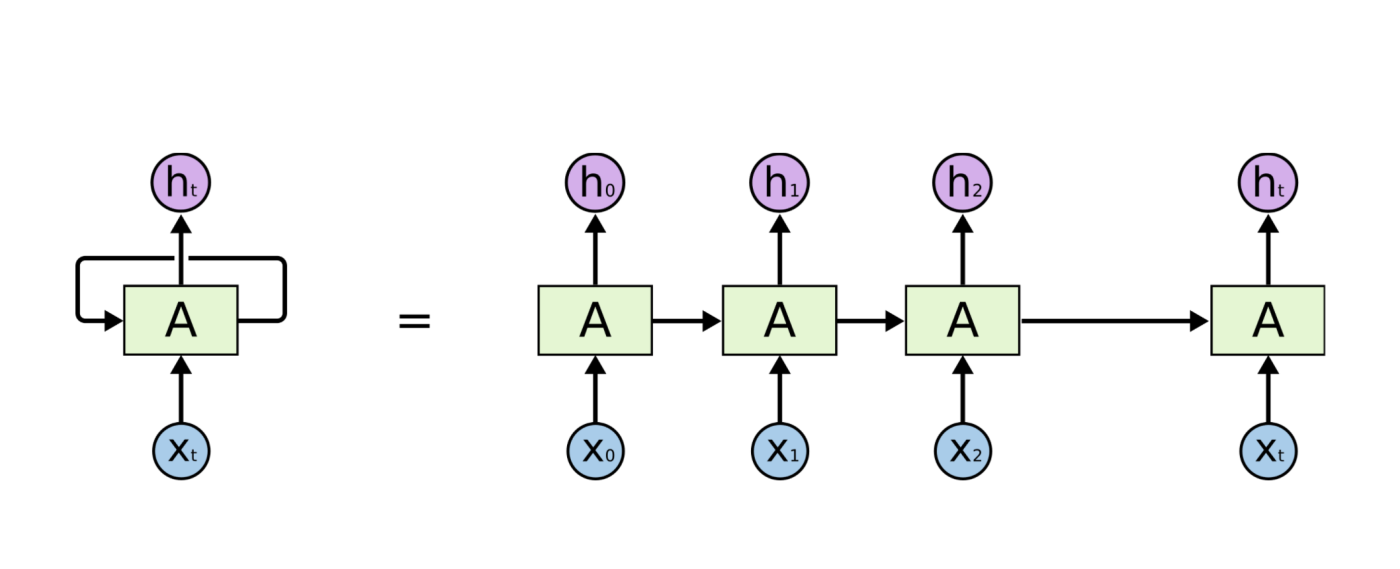
\includegraphics[width=0.9\textwidth]{images/ch2/02RNN.png}
    \caption{Architecture of a RNN.  Original image from \cite{NN}.}
    \label{fig:02RNN}
\end{figure}

CNNs are the last type of neural networks and are typically used for computer vision applications. The architecture of a typical CNN can be found in Figure \ref{fig:02CNN}. Unlike its predecessors, CNNs make the explicit assumption that inputs to the network will be images. This enables certain properties to be encoded into the architecture, making the forward pass more efficient while reducing the number of parameters.  More specifically, CNNs assume all inputs are arranged in three dimensions: height, width, and depth.  The height and width are simply the resolution of an image while the depth is the amount of color channels.  For example, a coloured image contains 3 channels (red, green, blue) while a grayscale image contains only one.  From this assumption, the weights of CNNs only need to be applied to specific locations, without the need of fully connected layers.  Furthermore, the input data will then be downsampled using pooling layers to extract the most important features while discarding the rest.  

\begin{figure}[h]
    \centering
    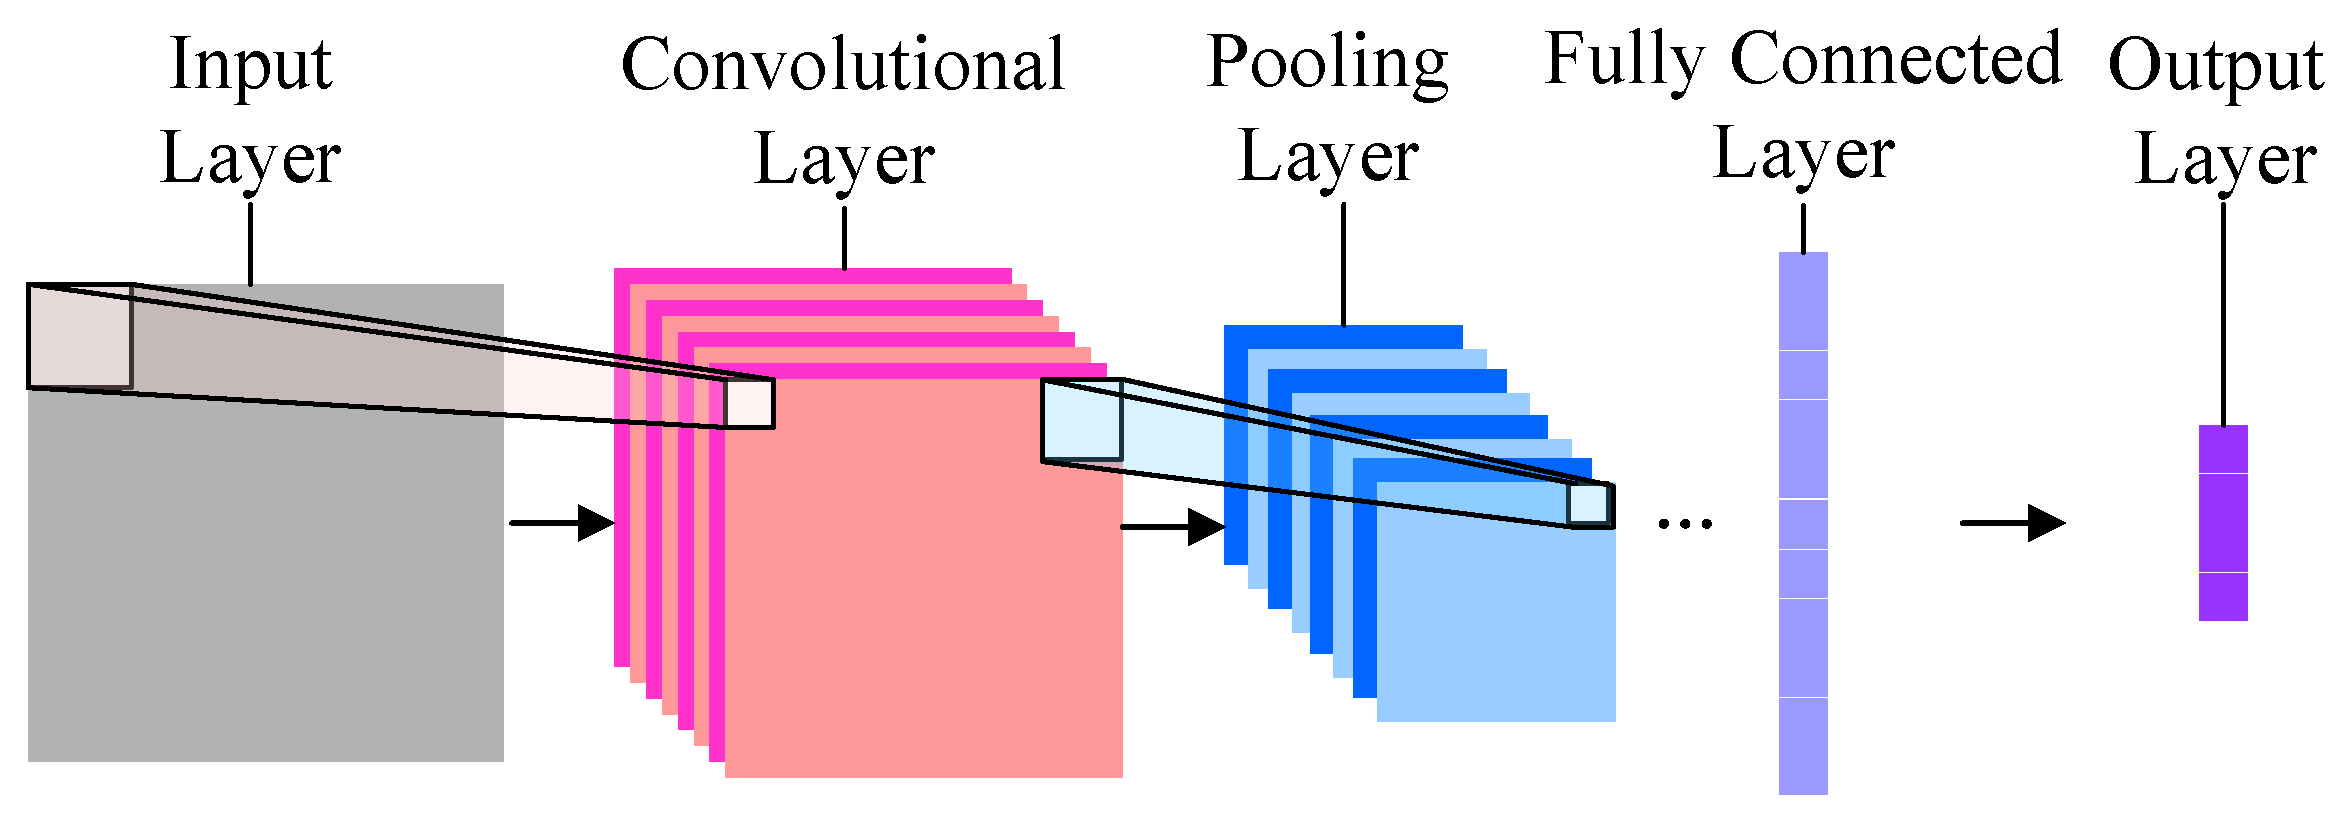
\includegraphics[width=0.9\textwidth]{images/ch2/02CNN.png}
    \caption{Architecture of a CNN.  Original image from \cite{NN}.}
    \label{fig:02CNN}
\end{figure}

In the process industry, CNNs can be leveraged as a soft sensor to measure variables using cameras. An example would be detecting the level of crude inside a primary separation vessel using the sight glasses, since traditional methods are not as effective.

Both CNNs and RNNs were not applied to the industrial project directly, but were provided to the reader as \textbf{advanced} methods for future projects that command exceptionally high predictive power, or computer vision soft sensing capabilities.  More information regarding RNNs and CNNs can be found in \cite{NN}.

\subsection{Linear Parameter-varying Models}
Linear parameter-varying models (LPV) were last type of ML models that were applied to the industrial pipeline. The motivation behind LPV models is twofold: i) Achieves a non-linear representation of the data using a combination of linear models; ii) Models different operating regimes of a process using different models.  The LPV model structure is identical to linear models with the exception that there are multiple linear models.  The number of linear models is a function of the non-linearity of the system, the number of operating regimes, and the amount of available data.  

Figure \ref{fig:02LPVexample} shows an example of fitting multiple linear models to approximate a non-linear system. Two separate approaches were used: 3-model approach and 6-model approach.  Performance wise, the 6-model approach is far superior. However, the 6-model approach uses twice as many models resulting in a significantly higher maintenance and ownership cost.  Additionally, the individual model performance for the 6-model approach may experience high variance if low amounts of data are present at certain points.  If performance is of utmost importance and data is abundant, a large number of linear models could be used.  Otherwise, a LPV model with a lower amount of models is adequate.

\begin{figure}[h]
    \centering
    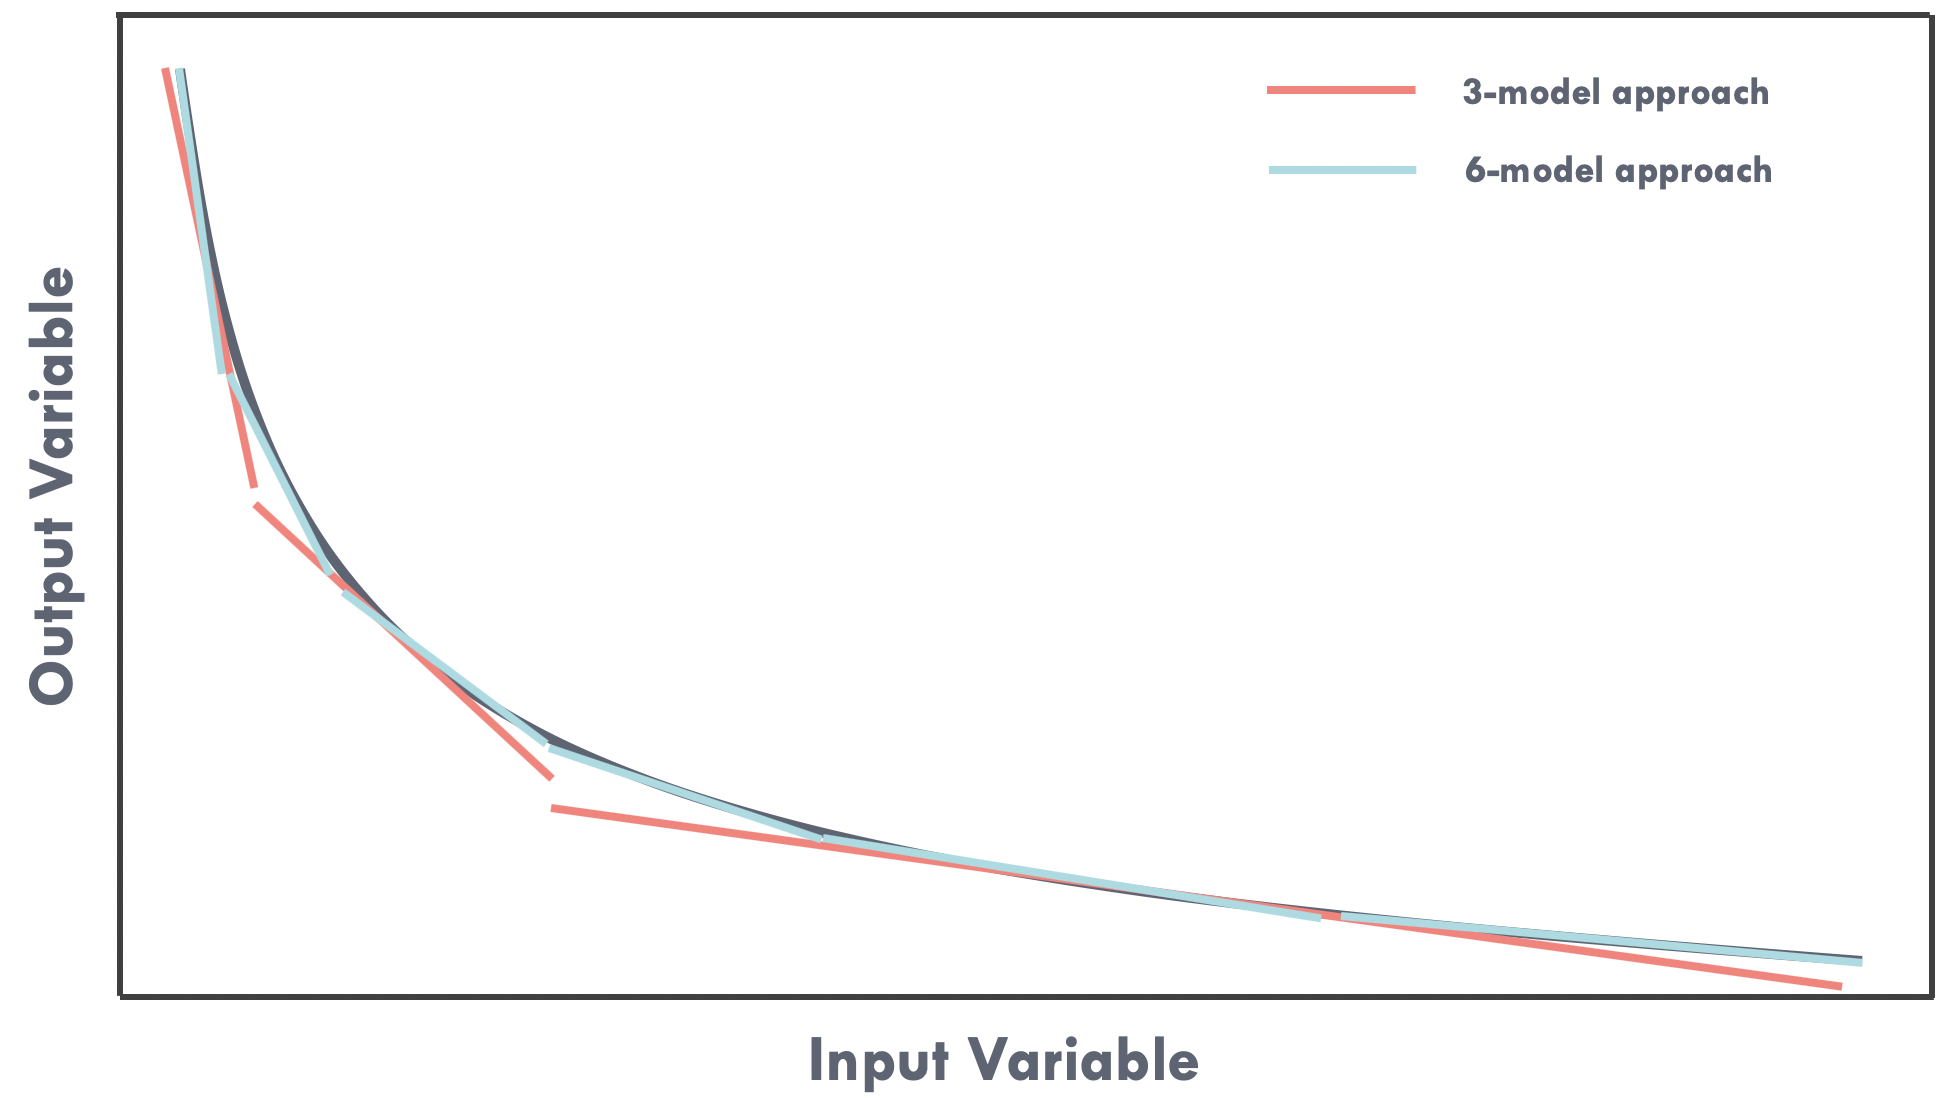
\includegraphics[width=\textwidth]{images/ch2/02LPVexample.jpeg}
    \caption{Fitting a non-linear function using multiple linear models.}
    \label{fig:02LPVexample}
\end{figure}

Clustering techniques can be used to identify distinct models for large MIMO systems containing multiple operating regimes and/or where non-linearity is not easily visualized.  Table \ref{tab:08cluster1_cluster2_reg} and Figure \ref{fig:08LPVModels} shows the application of a 2-model LPV model onto the industrial pipeline for the two separate operating regimes.  The original data set was first segregated into two clusters using DBSCAN.  Then, separate linear models were built for each cluster. During model testing, the Euclidean distance of new samples to the centroids of each cluster is computed to determine which linear model should be used for prediction. In terms of performance, the LPV model was able to achieve very similar performance metrics compared to the other non-linear models.  Additionally, the LPV models are more representative of the process in terms of control because each model (for each operating regime) has unique weights and constraints. For control, this is especially beneficial.  For example, if pump A was never used for operating regime B, the model would be highly inaccurate if the control system recommended its operation.  Using LPV models, explicit constraints can be placed to prevent such a scenario, as shown in the LPV section in Appendix A.

The training and deployment procedure for using a LPV model in an arbitrary process is shown in Figure \ref{fig:02lpv_architecture}.  Starting from the top, historical data for the process is first clustered into $n$ data sets.  Here, $n$ can be pre-defined using subject matter knowledge, or can be found using DBSCAN.  After segregation, each cluster should have enough data to effectively identify useful linear models.  Finally, the data sets are used to identify linear models.  Each model will have unique constraints to enhance the representation of the physical process.  Deployment-wise, new measurements are obtained from field sensors and are sent to the LPV model.  Then, the Euclidean distance (or desired distance metric) between the new measurement and the centroids of each model are calculated. The model exhibiting the lowest distance will be used for prediction. However, if the distance between the new measurement and the closest centroid is too large, the measurement will be labeled as anomalous instead.

\begin{figure}[h]
    \centering
    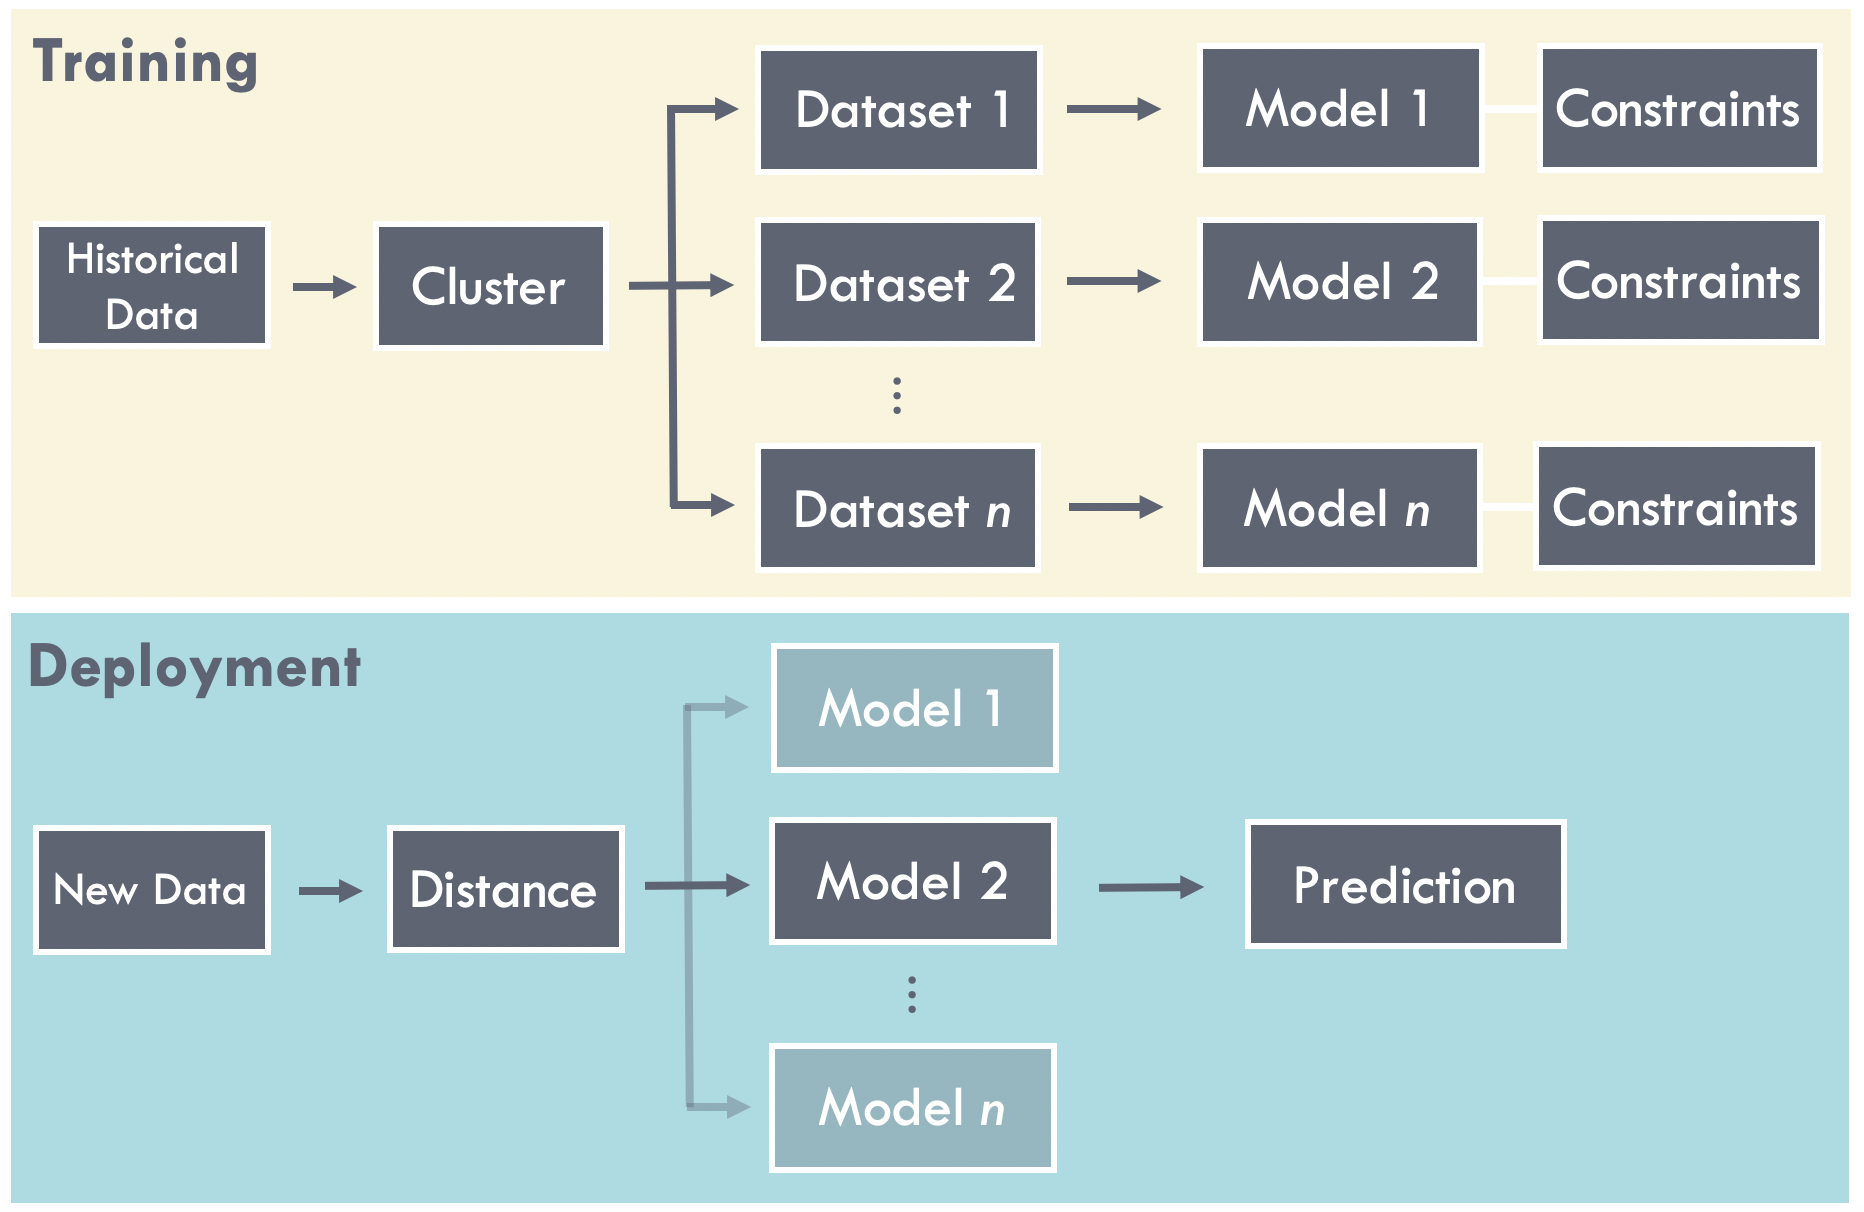
\includegraphics[width=\textwidth]{images/ch2/02lpv_architecture.jpeg}
    \caption{Architecture of the LPV model during training and implementation}
    \label{fig:02lpv_architecture}
\end{figure}

\subsection{USIS: Uniform Sampling Incremental Supervised learning}
A major selling point of ML solutions is their promise of being adaptive. Because of the way ML solutions are updated (gradient descent), adaption can easily be incorporated in a natural and biological way. Figure \ref{fig:02GradDesc} shows an intuitive representation of the gradient descent algorithm.

\begin{figure}[h]
    \centering
    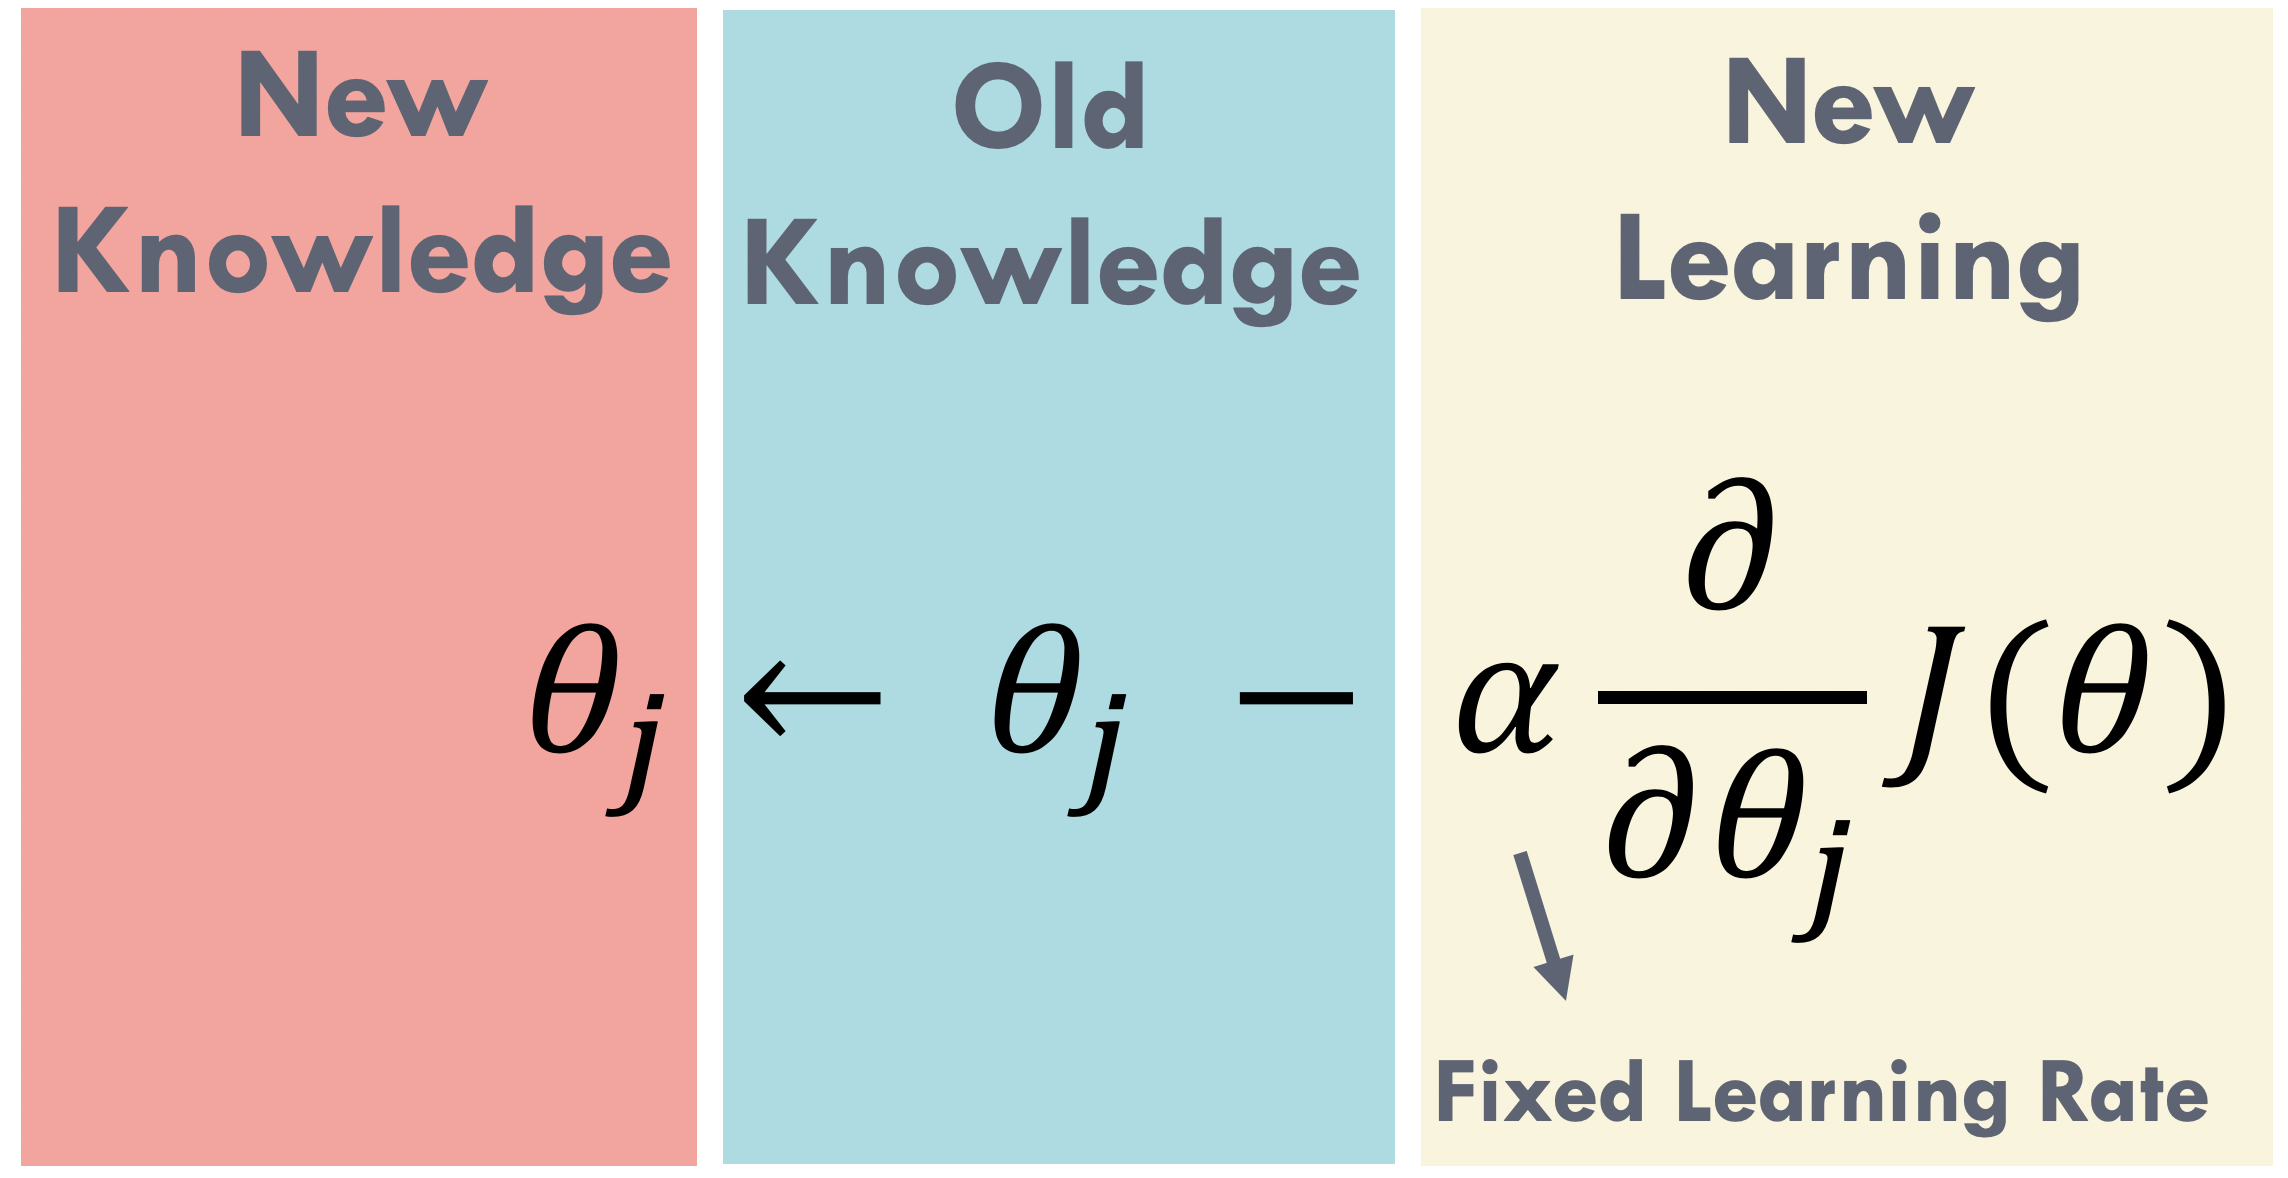
\includegraphics[width=0.75\textwidth]{images/ch2/02GradDesc}
    \caption{An intuitive representation of gradient descent.}
    \label{fig:02GradDesc}
\end{figure}

During an update step, the new knowledge is intuitively the old knowledge adjusted by new learnings.  The new learnings are typically multiplied by a fixed learning rate, $\alpha$. From this, the new knowledge is always biased towards the most recent experience, giving ML solutions an adaptive characteristic.  Adaptive ML can be implemented in two forms: online learning or incremental learning. Online learning refers to the ML models being updated after each prediction and can be understood mathematically as stochastic optimization. Common applications of online learning can be found in search optimization for web pages, where millions of data points are generated per minute. Online learning is not suitable for process control applications due to three reasons: catastrophic interference (i.e., tendency of neural networks to completely and abruptly forget previously learned information upon learning new information \cite{cat_int}), sequential noisy data decimating model accuracy, and insufficient incoming data to identify representative models for useful applications.  In adaptive ML, incremental learning is the preferred choice for process control applications due to its reduced randomness.  Incremental ML works by creating a data cache, and then updating the model using all data from the cache simultaneously after a fixed interval.  By doing so, the models will be updated much slower and the gradient of the loss function is an average of many examples, a method similar to semi-stochastic optimization.

\subsubsection{Motivation}
Incremental learning still falls short in terms of catastrophic interference (also known as catastrophic forgetting). This is especially a problem for the process industry, where operating conditions may be prolonged for many months before a switch is made. Because ML solutions are biased towards the most recent experiences, past experiences will be forgotten and the model will perform poorly if faced with old conditions after a long time. 

The uniform sampling incremental supervised learning (USIS) algorithm was proposed to overcome this issue and to enhance data efficiency for adaptive ML techniques.  USIS is a combination of adaptive resonance theory, uniform sampling, and experience replay (from reinforcement learning theory), where each update step is outlier free, data is efficiently used many times, and data is uniformly sampled across the distribution of the model to prevent catastrophic interference.

The simplified adaptive resonance theory (ART) architecture is shown in Figure \ref{fig:02art}. ART was originally proposed to prevent disrupting existing knowledge during learning of new knowledge.  In ART, the comparison field first allocates the input vector to the best match model in the recognition field based on a similarity metric, $s$.  Then, the similarity between the input vector and the closest matching model is compared to the vigilance parameter, $\nu$.  If $s > \nu$, the model weights will be adjusted using the new input vector.  Otherwise, the input vector is used to initiate a new model.  The vigilance parameter has significant influence on the overall system.  Intuitively, higher vigilance produces highly detailed memories (many specialized models), while lower vigilance creates generalized memories (fewer, generalized models) \cite{art}.

\begin{figure}[h]
    \centering
    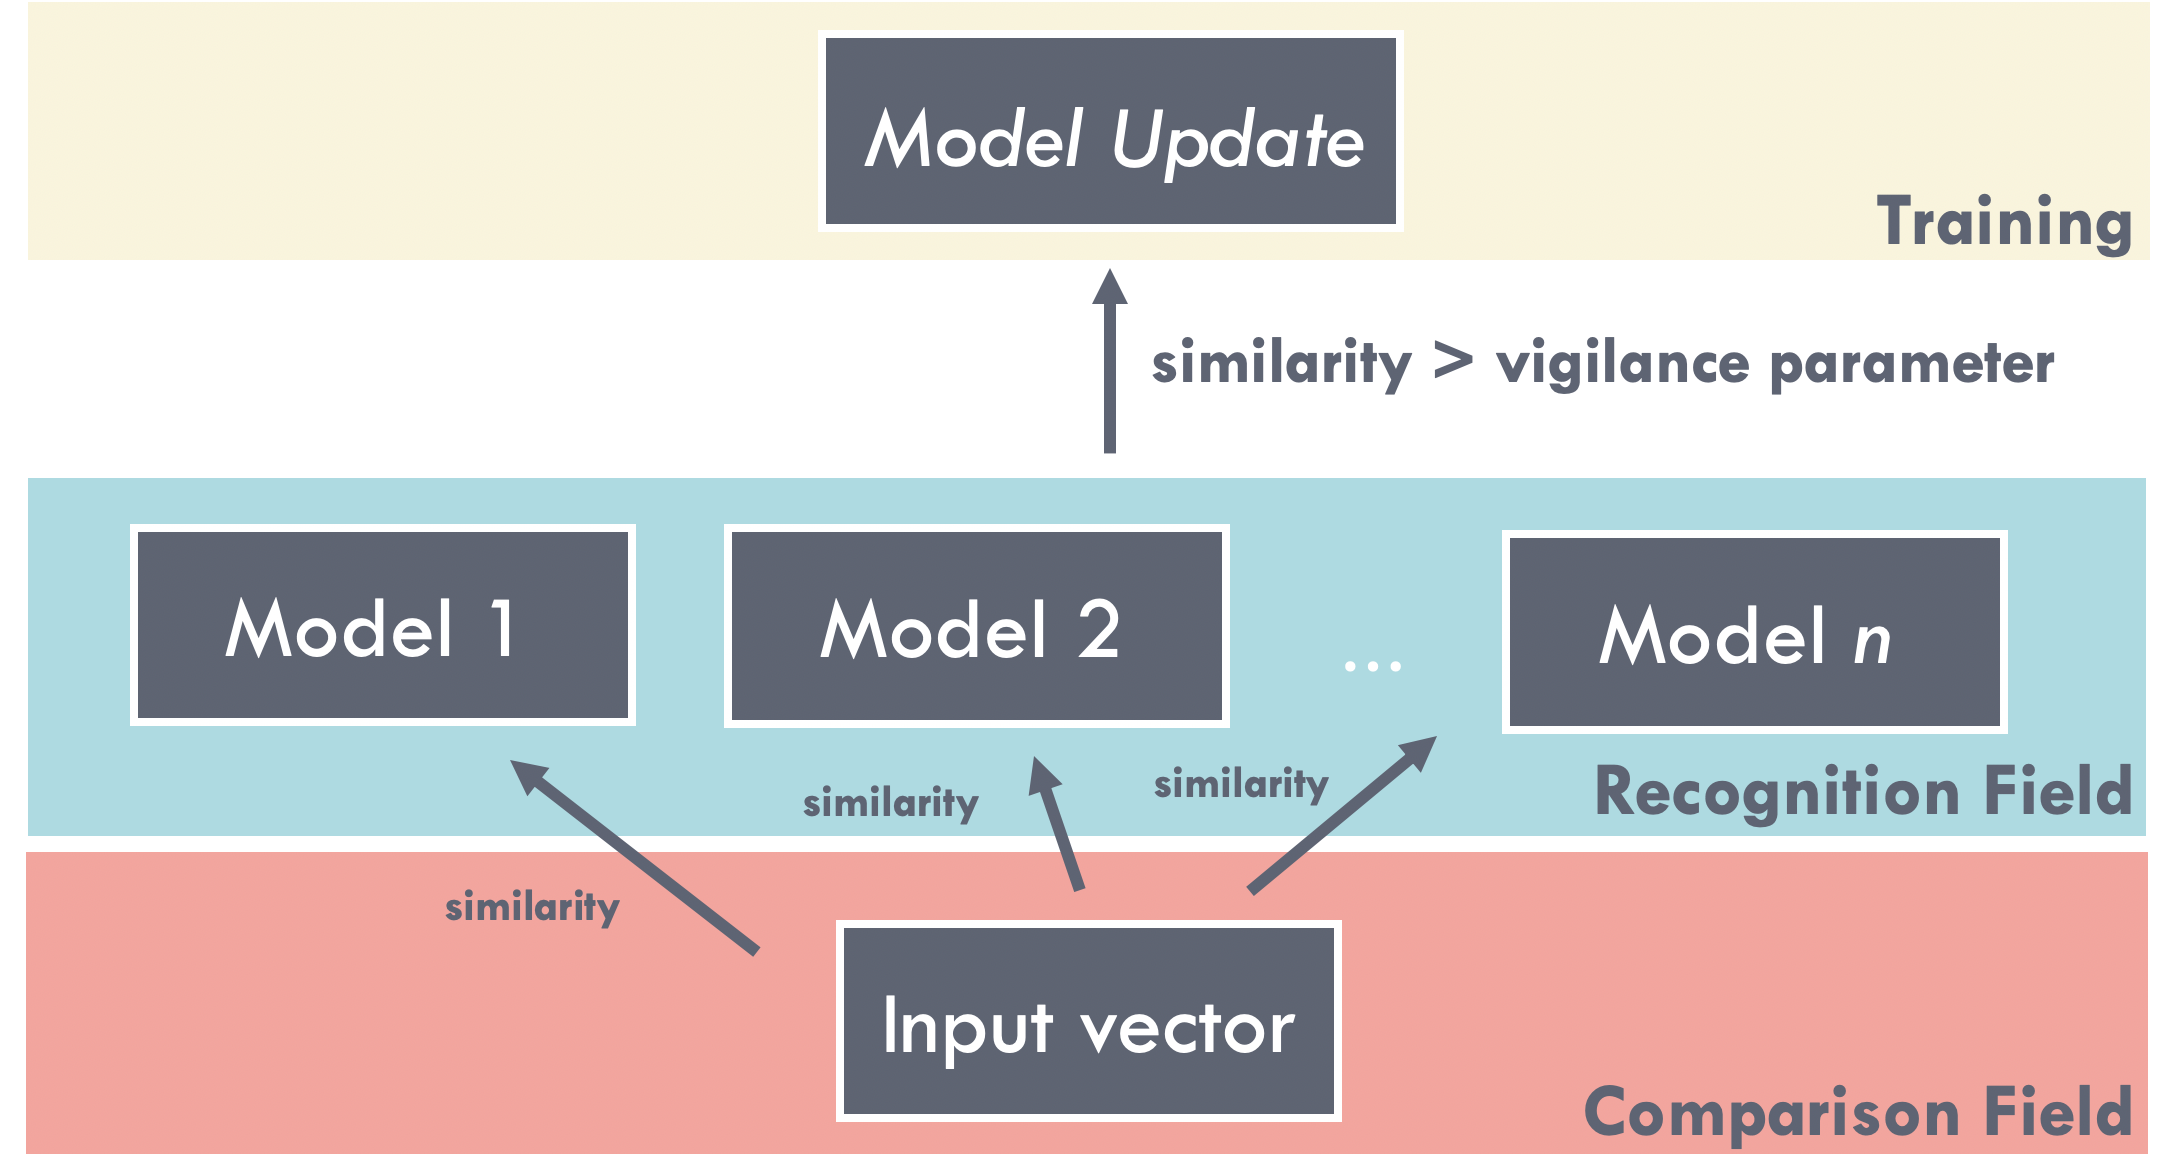
\includegraphics[width=\textwidth]{images/ch2/02art.jpeg}
    \caption{The simplified adaptive resonance theory architecture.}
    \label{fig:02art}
\end{figure}

Uniform sampling is a random sampling method where proportions of each desired group are forced to be sampled equally. For example, imagine a pump data set used to predict for the pump RPM given an input current.  The pump RPMs range between 0 - 1000 and the accuracy of the model is important across all values; however, the data set is significantly biased towards the 900 - 1000 RPM range, with only few data points in other regions. To ensure the model has acceptable performance across all values, the data set can be binned and equal amounts of data from each bin are sampled during the update step.  In the context of process control where data typically remain constant over long periods of time, uniform sampling can guarantee data variety during an incremental learning update step.

Lastly, experience replay is a method that gained popularity when it was first introduced to reinforcement learning to improve data efficiency and break temporal correlations \cite{dqn}. In experience replay, data (or experiences) are accumulated over time and are stored in a buffer.  During an update step, data is randomly sampled from the buffer to break temporal correlations that could potentially bias the models towards the most recent experience.  Additionally, data within the buffer can be re-used many times rather than being discarded after one update. Only after many time steps are the oldest memories removed from the buffer. An biological interpretation behind the algorithm is that humans create memories of past experiences.  Over the span of our lives, the same experiences are replayed many times; subconsciously when we eat, study, sleep, etc.  In doing so, humans can learn new experiences without catastrophically forgetting about past experiences; however, after an elongated period of time, distance unimpactful memories are forgotten.

By combining the advantages of the previous three topics, a new adaptive, outlier-robust, and data efficient algorithm catered towards the process control industry was developed.

\subsubsection{USIS Algorithm}

Figure \ref{fig:02USIS} shows the key steps for the USIS algorithm.  Initially, $n \geq 1$ models are present to model the system.  For input vectors in $n \geq 2$ systems, the distance $d$ between the input vector and the centroid of the data for each model is computed. This step is skipped for systems where $n = 1$ because only one $d$ is computed. The lowest $d$ is then compared to the neglect parameter, $\eta$ (opposite of vigilance parameter, $\nu$).  If $d \leq \eta$, the input vector will be added to the training archive (experience replay buffer) corresponding to the model.  Otherwise, the data point is transferred to the new model archive where data currently not belonging to any model is stored. In the new model archive, new models will be generated and added to the existing system of models after enough similar data is accumulated. Likewise, the training archives are used to incrementally update all models after a certain amount of data or time elapsed. During an update step, the archive data will be blended with additional uniformly sampled data from the historical archive (experience replay buffer) to avoid catastrophic interference. 

\begin{figure}
    \centering
    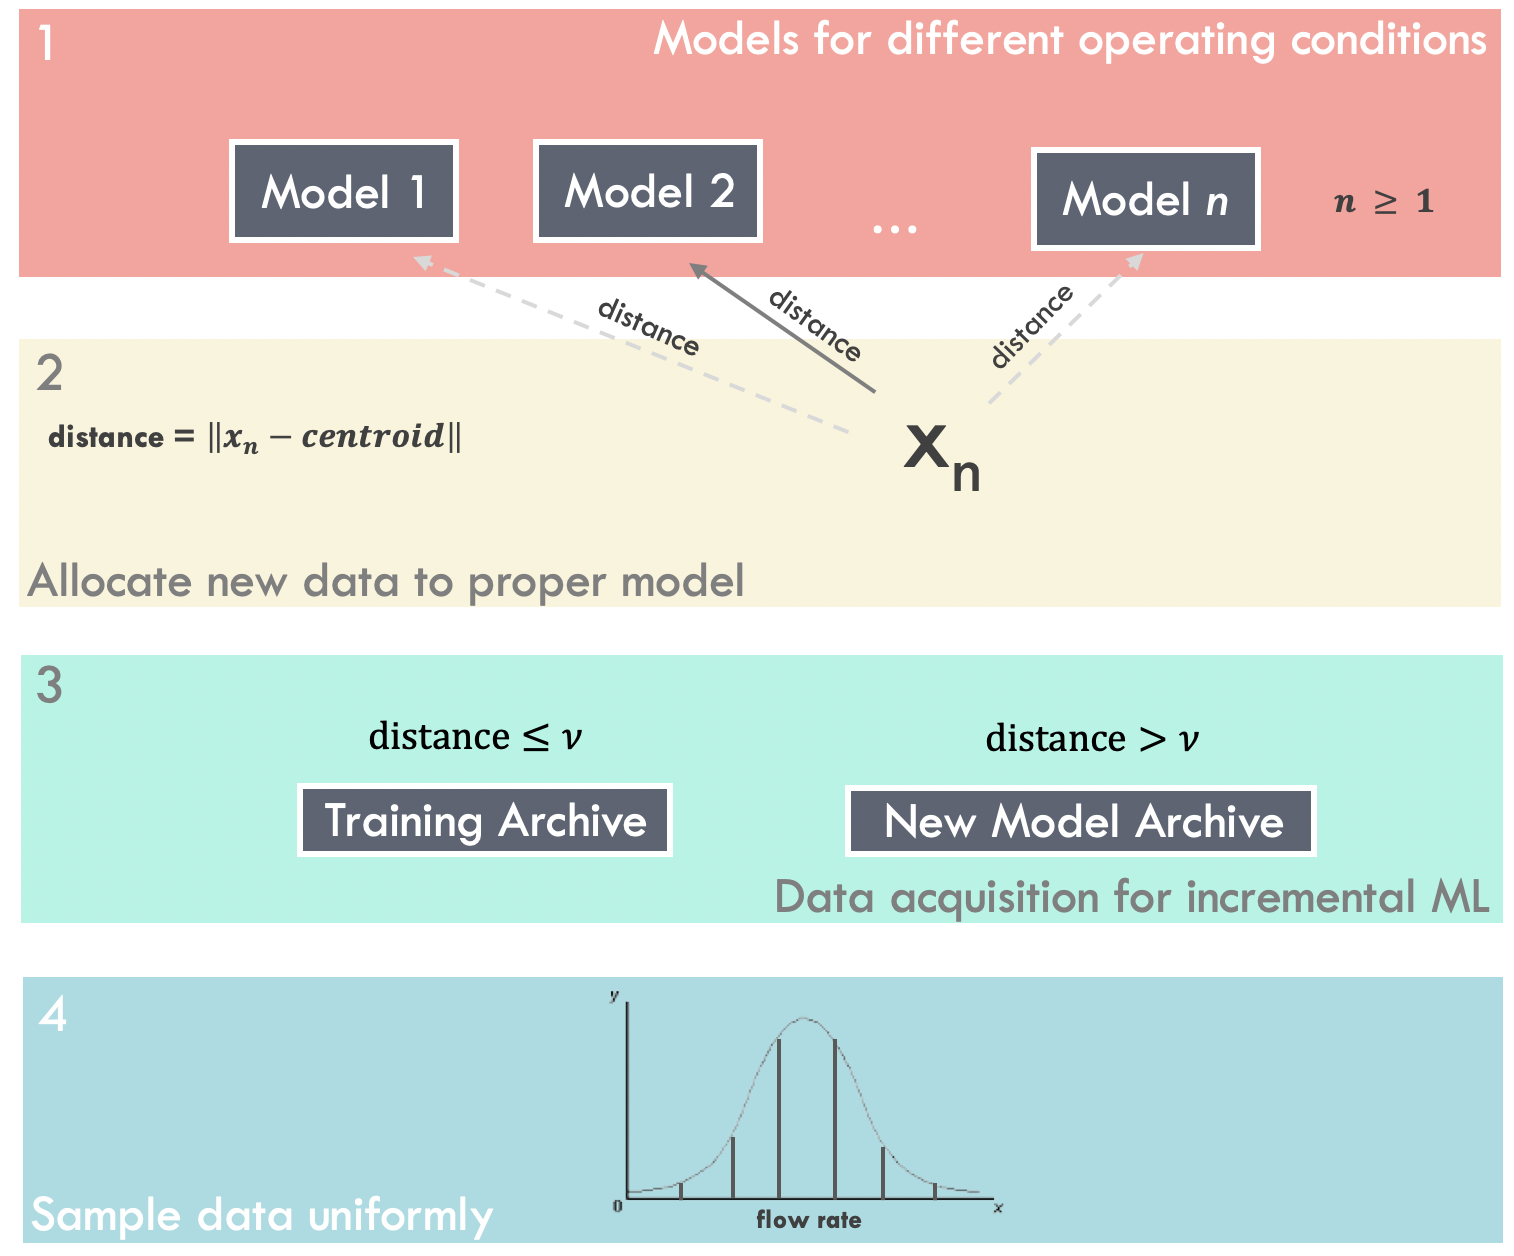
\includegraphics[width=\textwidth]{images/suncor/08IncrementalLearning.png}
    \caption{A brief visualization of the USIS algorithm.}
    \label{fig:02USIS}
\end{figure}

To enhance clarity of each update step, the data storage structure of USIS is shown in Figure \ref{fig:02USISData}. Before an update, the bins of each model must be defined.  The bins are typically defined by dividing the distribution of the predicted variable.  Bins can be narrower around regimes with abundant data, and wider for regimes lacking data.  During an update step, all data from the training archive alongside some sampled data from the historical training archive are blended together and fed into the gradient descent step for model updates.  Typically in process control applications, systems tend to linger around certain set points for many time steps.  Given this characteristic, the data in the training archives, consisting of $m$ training examples, typically belong to the same bin.  To avoid catastrophic interference when learning on elongated periods of similar operating conditions, $m$ examples of data from each bin in the historical archive is also sampled and assimilated with the training data when performing update steps. After the updates, all training archives are emptied by transferring the data into the historical archives.  When the historical archives get sufficiently full, the oldest data (or memories) are deleted.

\begin{figure}[h]
    \centering
    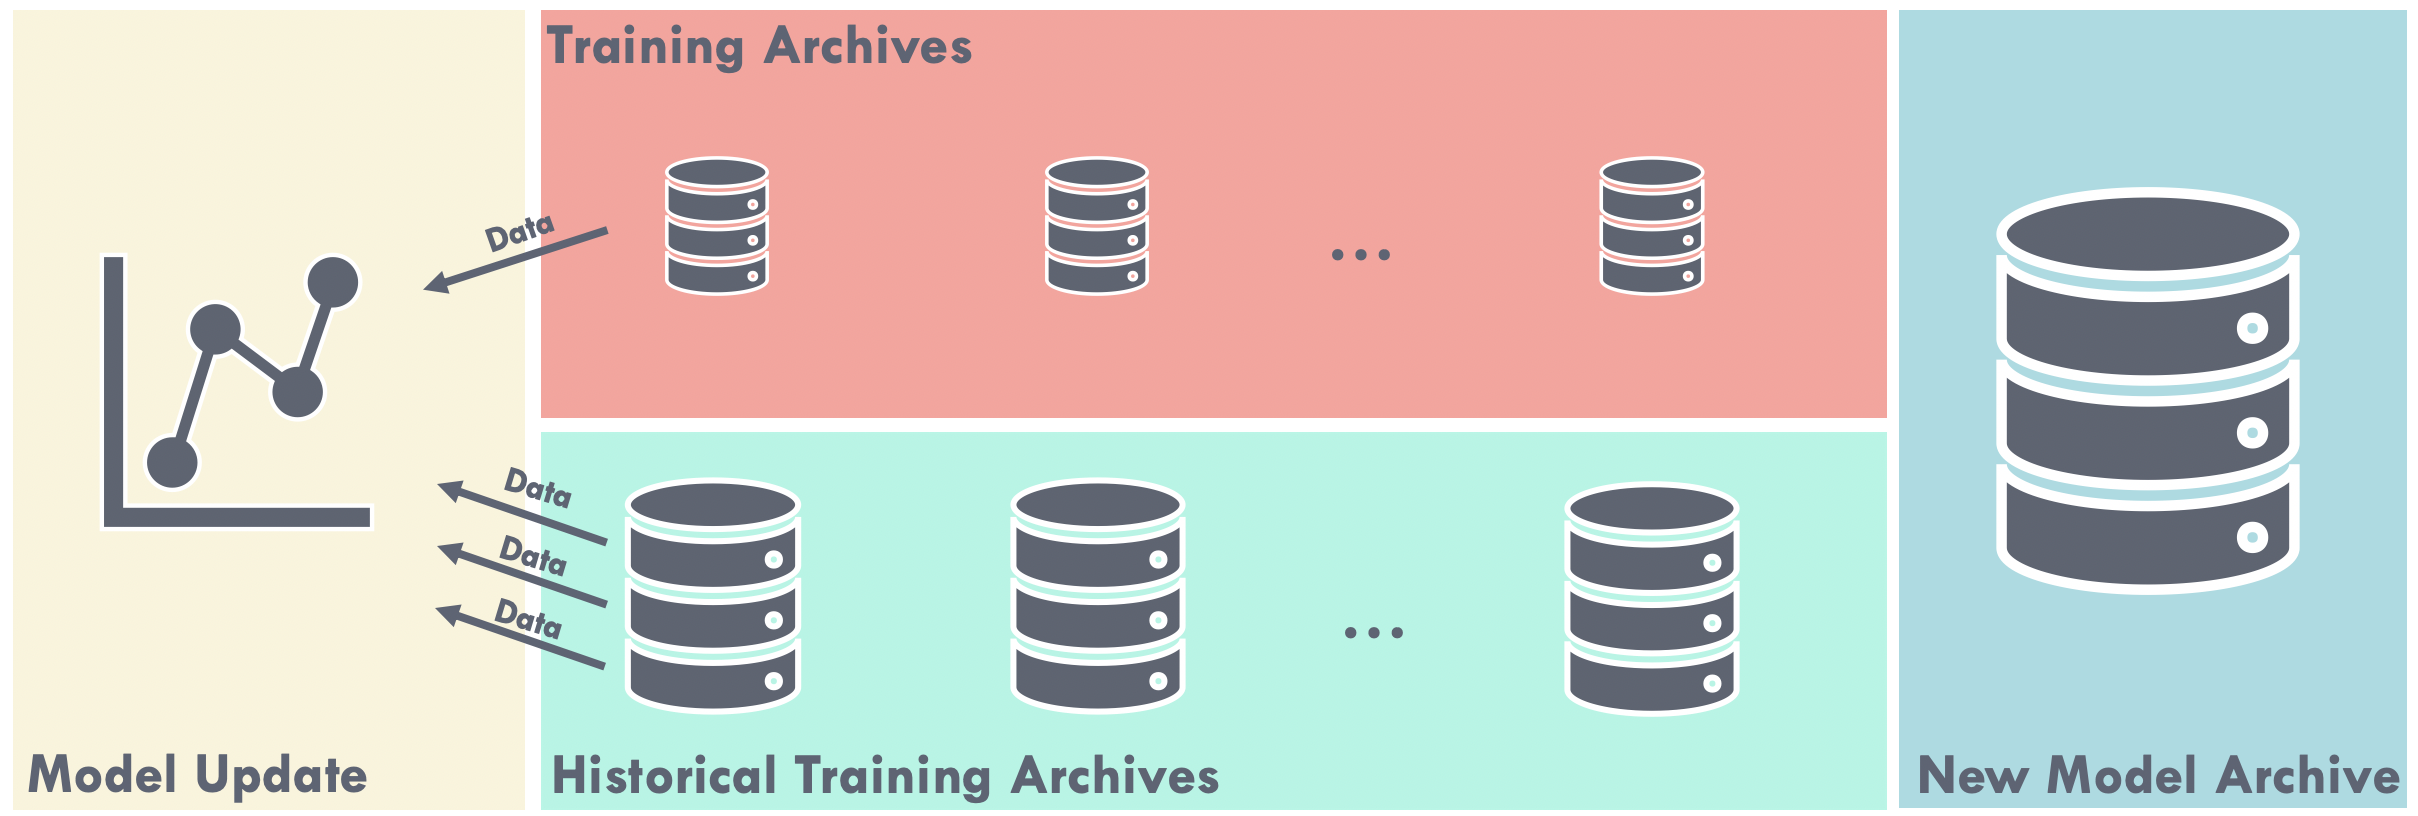
\includegraphics[width=\textwidth]{images/ch2/02USISData.jpeg}
    \caption{Data storage structure of USIS.}
    \label{fig:02USISData}
\end{figure}

The full USIS algorithm is shown in Figure \ref{fig:02USIS_Complete}.  There are five main tuning parameters of the USIS algorithm: i) when to update models; ii) bin size for each model; iii) neglect parameter; iv) distance metric; v) replay buffer size.

\begin{itemize}
    \item \textbf{i) Model Updates: } Common strategies for model updates are periodically, by example size, or when models exhibit large errors.  The first two are proactive methods, while the last is a reactive method.  In the periodically updating method, the models are automatically updated after a certain time has elapsed (e.g., update every 24 hours). Updates by example size refers to model updates after a certain amount of data is accumulated in the training archive. Only the model with adequate amounts of data is updated. For these two methods, there should not be a significant time gap between updates because updates may lead to excessive model changes otherwise.  Since this method is automated, significant model changes could potentially lead to sudden performance changes, jeopardizing production safety.  Model updating after large errors have incurred is the last method.  Here, the models are updated after an error threshold has been exceeded.  Compared to the previous methods where smooth update steps are performed, this method introduces significant changes to the model. Systems with highly noisy data and require inordinate amounts of manual data processing will benefit from this update style because completely automated updates may lead to model divergence.

    \item \textbf{ii) Bin size: } The bin size of each model should be tuned so the important sections  of the predicted variable can be properly predicted for each model. Additionally, the bin can be narrower for sections where abundant data is available and wider for sections where data is sparse.
    
    \item \textbf{iii) Neglect parameter: } Neglect determines the specialization of each model.  High neglect creates fewer generalized models, while low neglect produces many specialized models.  For highly non-linear multi-modal systems, low neglect may be the preferred choice; however, the initial setup and cost of ownership for such a system could potentially be high if automated updates are not implemented/feasible. On the other hand, high neglect systems are cheaper to maintain due to the reduced number of models, but the accuracy may suffer.  Picking a proper neglect parameter represents the trade-off between accuracy and complexity.  A general rule of thumb for the neglect parameter would be the radius of the cluster.  For example, $\eta$ for a cluster identified using DBSCAN would be its $\epsilon$ value.
    
    \item \textbf{iv) Distance metric: } The Euclidean distance between the input vector and the historical data is the recommended choice; however, other distance metrics can be used for specialized applications.
    
    
    \item \textbf{v) Replay buffer size: } The replay buffer size can also be tuned to adjust when old memories are no longer relevant (intuitively, forgetting older memories).  For processes where operating conditions are changing frequently, it would be beneficial to have smaller replay buffers to avoid learning on obsolete data.  Replay buffers can also have an adaptive size depending on the current prediction error as proposed in \cite{eff_of_er}; however, such a method is still embryonic and further exploration should be conducted before implementation.
\end{itemize}

\begin{figure}[h]
    \centering
    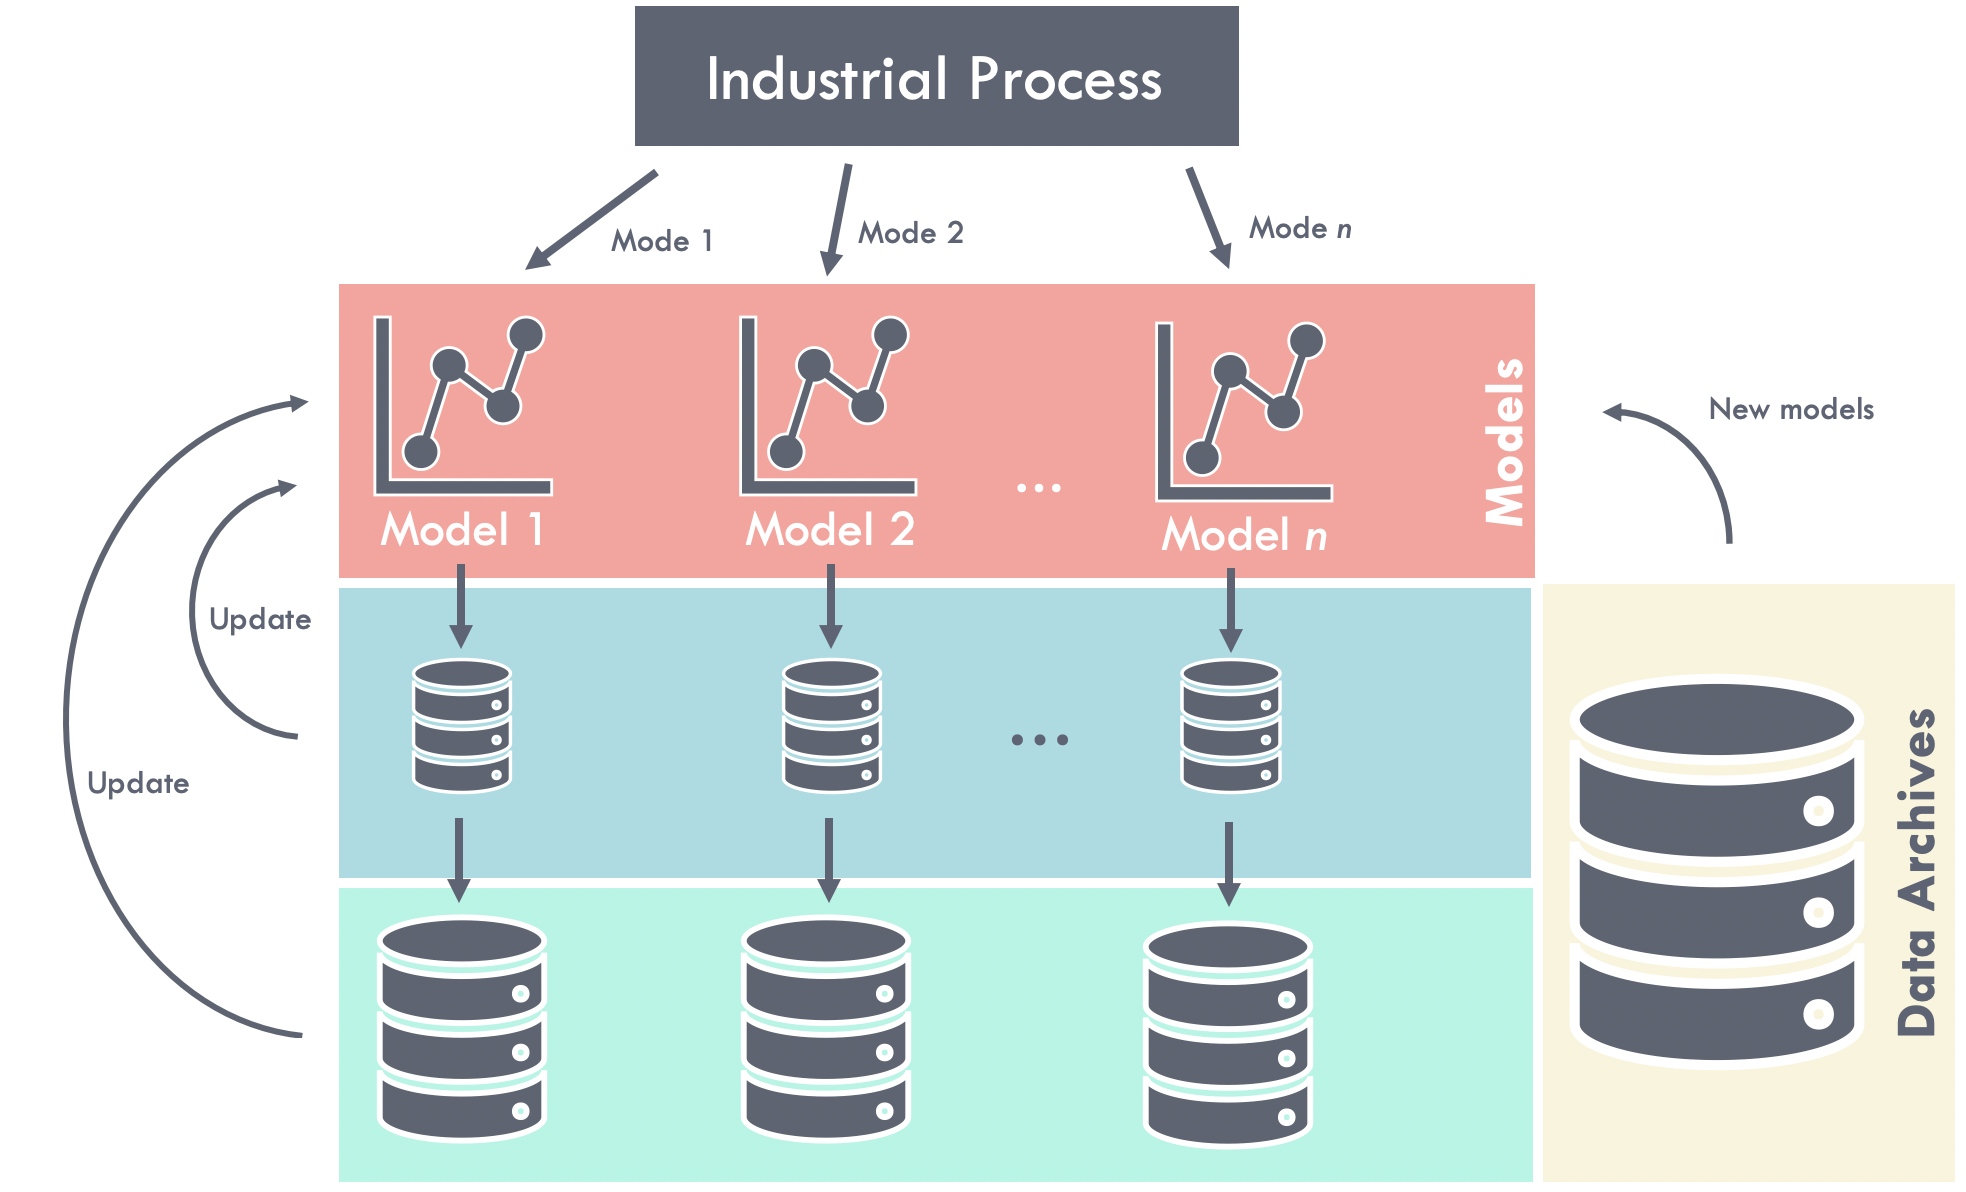
\includegraphics[width=\textwidth]{images/ch2/02USIS_Complete.jpeg}
    \caption{The complete USIS architecture.}
    \label{fig:02USIS_Complete}
\end{figure}

Uniform sampling in USIS can also be swapped out for importance sampling, where high error examples are prioritized for the next sampling cycle (motivation from \cite{prioritize_exp_replay}. In doing so, high error examples (biologically modelled as 'shocking' experiences) have higher probabilities of being recalled.  Intuitively, humans recall 'shocking' experiences more often. The method enhances accuracy in many reinforcement learning applications \cite{dqn, er1, er2}, although, such a method may prioritize noisy, near-outlier data points in process control applications and introduce model divergence.

\section{Discussion: Cheaper, More Accurate, and Adaptive?}

Machine learning has promised cheaper, more accurate, and adaptive solutions for industries around the world.  However, applying ML solutions naively into the process control industry yields no significant value due to various unique factors in process control data.  So far in this chapter, different data pre-processing methods catered towards the process industry were introduced.  General ML methods and their applicability were correlated to the process control industry. By innovatively combining parts of separate algorithms, a new algorithm catered towards the process industry, USIS, was also introduced. USIS is an adaptive, outlier-free, model structure that can be used to model a process with many operating conditions while avoiding catastrophic interference. But are these solutions truly cheaper, more accurate, and adaptive? 

The comparison between ML prediction solutions and traditional methods is shown below for common areas where ML is implemented today:

\begin{itemize}
    \item \textbf{Cheaper: } ML soft sensors will definitely be cheaper for difficult-to-measure process variables where lab test must be conducted.  Conducting lab measurements may cost up to hundreds of thousands per year if frequent measurements are required.  Initial cost for soft sensors may be high because a ML expert must collaborate with process operators to first develop the soft sensor(s); however, on-going costs for this application is minuscule.  Soft sensors for prediction of variables that are difficult to measure are definitely cheaper than buying a highly advanced physical sensor.  Lastly, prediction applications used for operator training or forecasting should be significantly cheaper compared to having a senior operator on shift explicitly to train a new operator or hiring a group of subject matter experts to forecast future production possibilities.
    \item \textbf{More Accurate: } Soft sensors used to predict lab measurements could yield high accuracy, but will never exceed lab measurements.  This is because lab data is used to train the soft sensor; hence, serving as a performance ceiling.  For soft sensors used to predict for difficult to measure process variables, the accuracy will depend on the quality of the data used to build the soft sensor.  Additionally, the accuracy vary from application to application.  For predicting for heights in a primary separation vessel using cameras and the sight glass, the accuracy can be extremely high.  On the other hand, predicting the density of a crude given highly noisy readings and poor input data may be nearly impossible.
    \item \textbf{Adaptive: } The adaptability factor of ML algorithms is purely dependent on available feedback.  For applications where immediate feedback is available, such as predicting for a continuously measured output variable, adaptability is trivial.  However, ML solutions cannot adapt for tasks where no feedback exists.  One example of a non-adaptive ML application would be soft sensors for prediction of lab measured process variables. If no additional lab measurements are taken after the soft sensor is live, it will never adapt.  Therefore, it is good practice to continue obtaining lab measurements seldomly to evaluate the soft sensor performance. For tasks requiring adaptation, ML solutions should be the preferred choice because human operators would have a hard time remembering all the historical data.
\end{itemize}

To summarize, ML prediction applications are generally cheaper compared to their traditional counterparts.  This is simply because applications that requires ML are typically expensive and are solved poorly using traditional approaches to begin with.  In terms of accuracy, ML solutions would not exceed the performance of a lab tested process variable; however, may surpass accuracy given representative data sets or unique applications.  Lastly, ML solutions can only adapt if proper feedback is available for the algorithm. 

\section{Highlights of ML Application onto a Pipeline}

The methods and algorithms in this chapter were applied onto an industrial pipeline\footnote{Many values are significantly rounded and/or omitted to maintain confidentiality of the project}\footnote{The algorithms are live as of May $7^{th}$, 2019 on one industrial pipeline. Work is being done to clone the project onto a second line.}.  The highlights of the implementation will be shown in this section.  For a detailed project report, please refer to Appendix A.

\subsection{Process Description}
Pipelines are critical assets for the transport of fluids safely and efficiently across long distances. Fluids include petroleum products, clean water, natural gas, sewage, and even beer. In Canada, over 97\% of petroleum products are shipped by pipeline alone.  Due to the mission critical nature of pipelines on society's success, ensuring its reliability and efficiency has global-scale impact.  Typical pipelines may contain hundreds of digital sensors littered across the pipeline.  Such information overload may be overwhelming for humans; however, ML methods benefit greatly from the abundance of data.  Here, an opportunity was discovered where ML methods can be applied to greatly increase the robustness and efficiency of the pipeline.  For phase one of the project, ML prediction models were built to create a digital twin of the pipeline for operator training programs and future optimization purposes.

A schematic of the pipeline is shown in Figure \ref{fig:02RM06A}.  The highly complex pipeline spans over 100 kms and carries two products, a lighter product and a heavier product. The two products are batched (i.e., rotate between sending each product) and each product is sent for approximately eight hours before switching to the other product. The American Petroleum Institute (API) gravity for the lighter and heavier products are roughly 40 and 20, respectively. For the rest of this chapter, the lighter and heavier product will be referred to as \textit{light crude} and \textit{heavy crude}, respectively. The pipeline is typically operated between 1800 bbl/h to 3050 bbl/h. 

\begin{figure}[h]
    \centering
    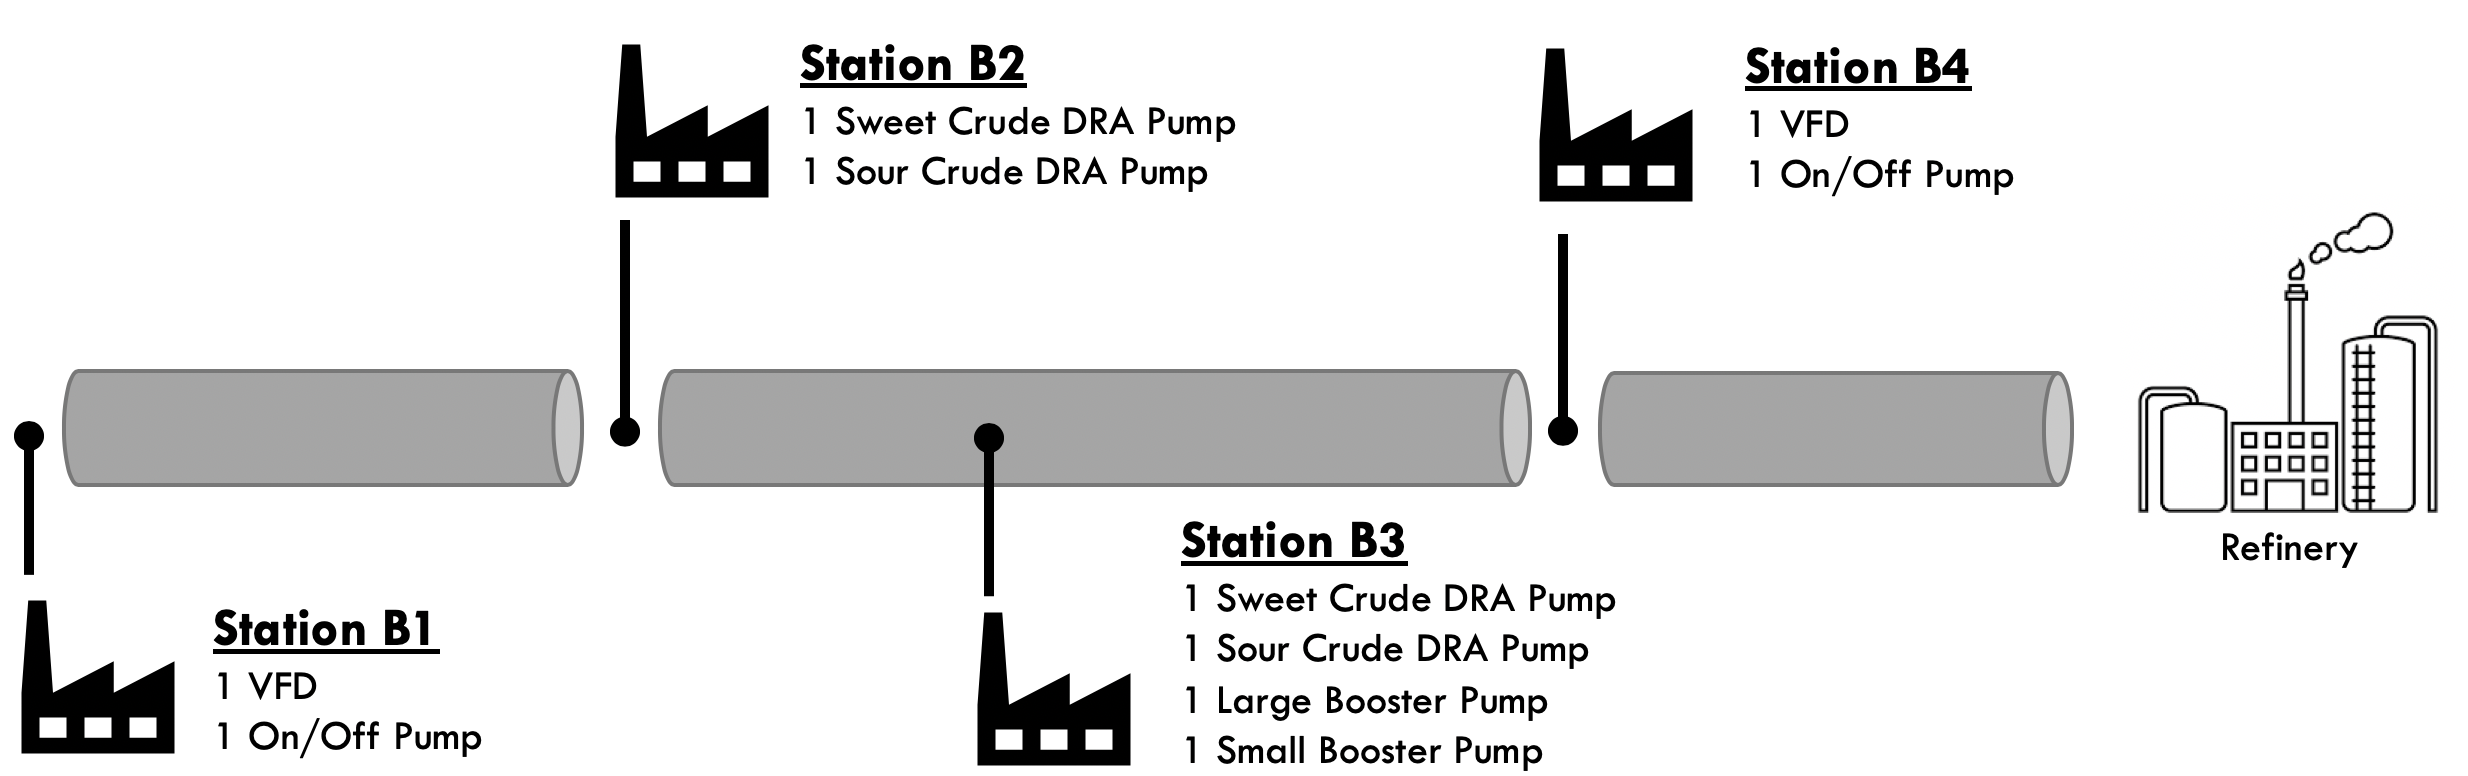
\includegraphics[scale=0.33]{images/suncor/08RM06A.png}
    \caption{Schematic diagram of Line B.}
    \label{fig:02RM06A}
\end{figure}

Equipment wise, Line B boasts eight pumps spread across four pump stations. Two pumps are variable frequency drives (VFD), while the rest are on/off pumps. Additionally, there are four drag reducing agent (DRA) injection pumps situated at the second and third pump stations. Each pump station contains a heavy crude and light crude DRA pump because the different crudes use different types of DRA.  The DRA is injected based on the product present at the pump station. 

\subsection{Data Pre-processing}
The industry sponsors initially provided a data set containing 899 tags and 525,601 data points for each tag.  The data pre-processing step was deconstructed into three phases for this project: pre-processing by subject matter experts, automated data pre-processing, and manual data pre-processing. The first two phases are typical of any machine learning project.  The third phase contains methods introduced in this chapter. Upon completion, an on-going iterative data pre-processing procedure continued until the end of the project to ensure industrial sponsors were satisfied with the model performance. The objective of the prediction models were to predict the \textbf{output flow rate} as a function of process variables.

The data was first pre-processed by experts within the sponsor's organization to remove useless tags such as alarm limits, fire detector status, and the sort.  After doing so, the amount of tags was reduced to 124.  The remaining data was sent into various automated data pre-processing algorithms to further remove redundant/insignificant tags.  The algorithms include: missing data removal, data imbalance analysis, and collinear analysis.  Missing data removal cleans up any NaN or empty values in the data set.  Data imbalance analysis inspects all categorical variables and removes heavily imbalanced tags where one class significantly dominates all other classes.  Lastly, collinear analysis identify heavily correlated columns and removes all but one to prevent redundancy in the data set. Total tags reduced to 65 after the automated feature selection.

Next, the manual pre-processing was conducted on the data set.  First, engineering knowledge was applied to the pre-processing step to remove segments of data where the process exhibits abnormal operating behaviour.  Then, the data at each pump station was shifted to incorporate time delays. In pipelines transporting incompressible fluids, pressure propagates down at the speed of sound (1480 km/h) \cite{fluid_mechanics}; therefore, all pressure variables were shifted with accordance to their distance to the output of the pipeline (shown in Table \ref{tab:02TimeToCC}.  Likewise, DRA also had time delay.  DRA must be transported down the entire pipeline to exhibit its full drag reducing effect.  From giving flow rates and the length of each segment of the pipeline, it was calculated that coating the entire pipeline required approximately ten hours.  Therefore, the first ten hours data corresponding to a set point change in DRA was removed to ensure the DRA's effect has been fully realized in the output flow rate data.

\begin{table}[h]
    \centering
    {\setstretch{1.2}
    \begin{tabular}{ p{6cm} | c | c | c | c}
             & B1 & B2 & B3 & B4 \\
        \hline
        Time to refinery at speed of sound in liquids (1480 m/s) \cite{fluid_mechanics}
        &  2.0 min  &  2.0 min  &  1.0 min  &  1.0 min  \\
    \end{tabular}}
    \caption{Time required for pressure changes at each pump station to be realized at refinery.}
    \label{tab:02TimeToCC}
\end{table}

Additionally, the temperature and DRA ppm measurements were highly noisy and were exponentially smoothed using Equations \ref{eq:08EWMA} to increase reliability.  The pre- and post-smoothed values of the DRA are shown in Figure \ref{fig:02DRA} to illustrate the effect of exponentially smoothing.

\begin{figure}
     \centering
     \begin{subfigure}[b]{0.9\textwidth}
         \centering
         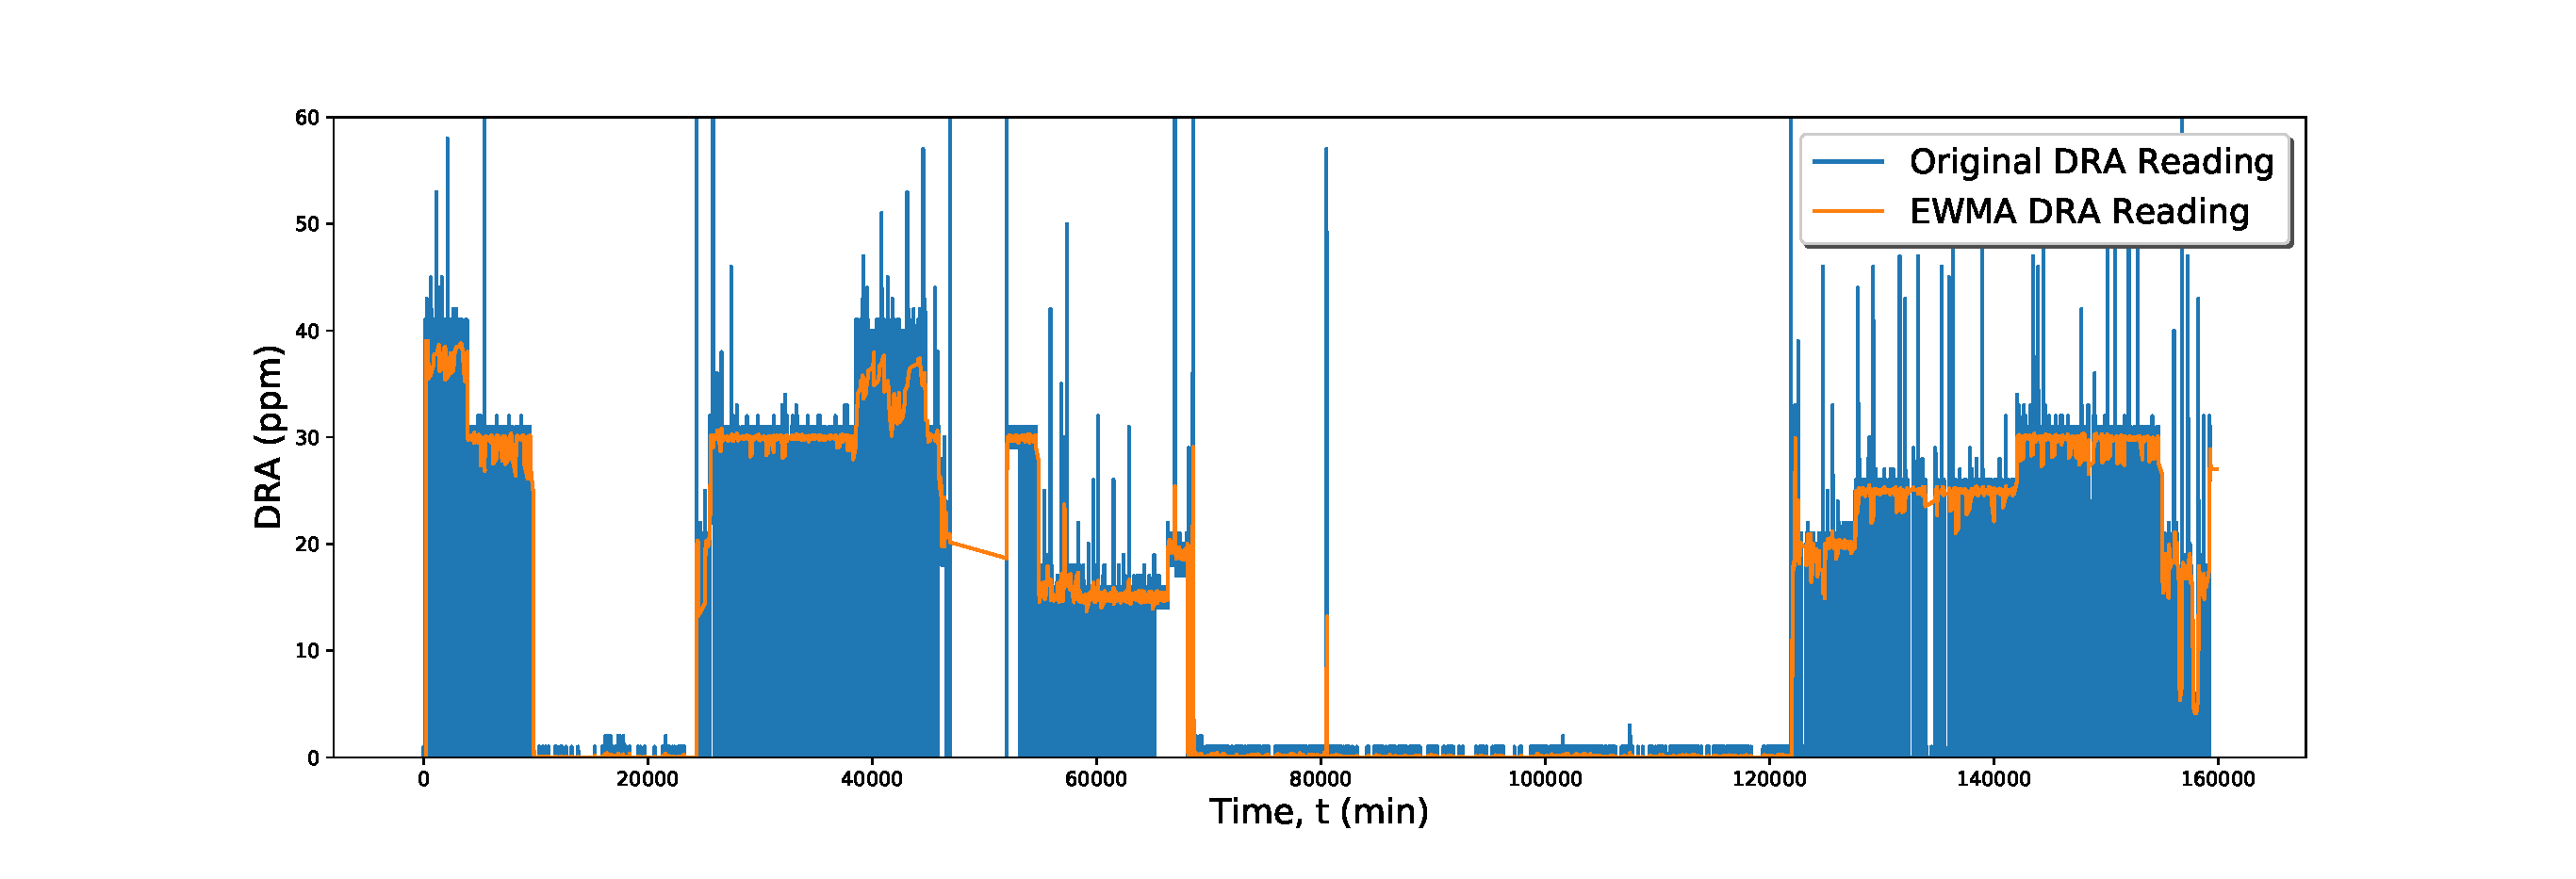
\includegraphics[width=\textwidth]{images/suncor/08CIGSour.eps}
         \caption{Station B2 heavy DRA sensor reading.}
     \end{subfigure}
     \begin{subfigure}[b]{0.9\textwidth}
         \centering
         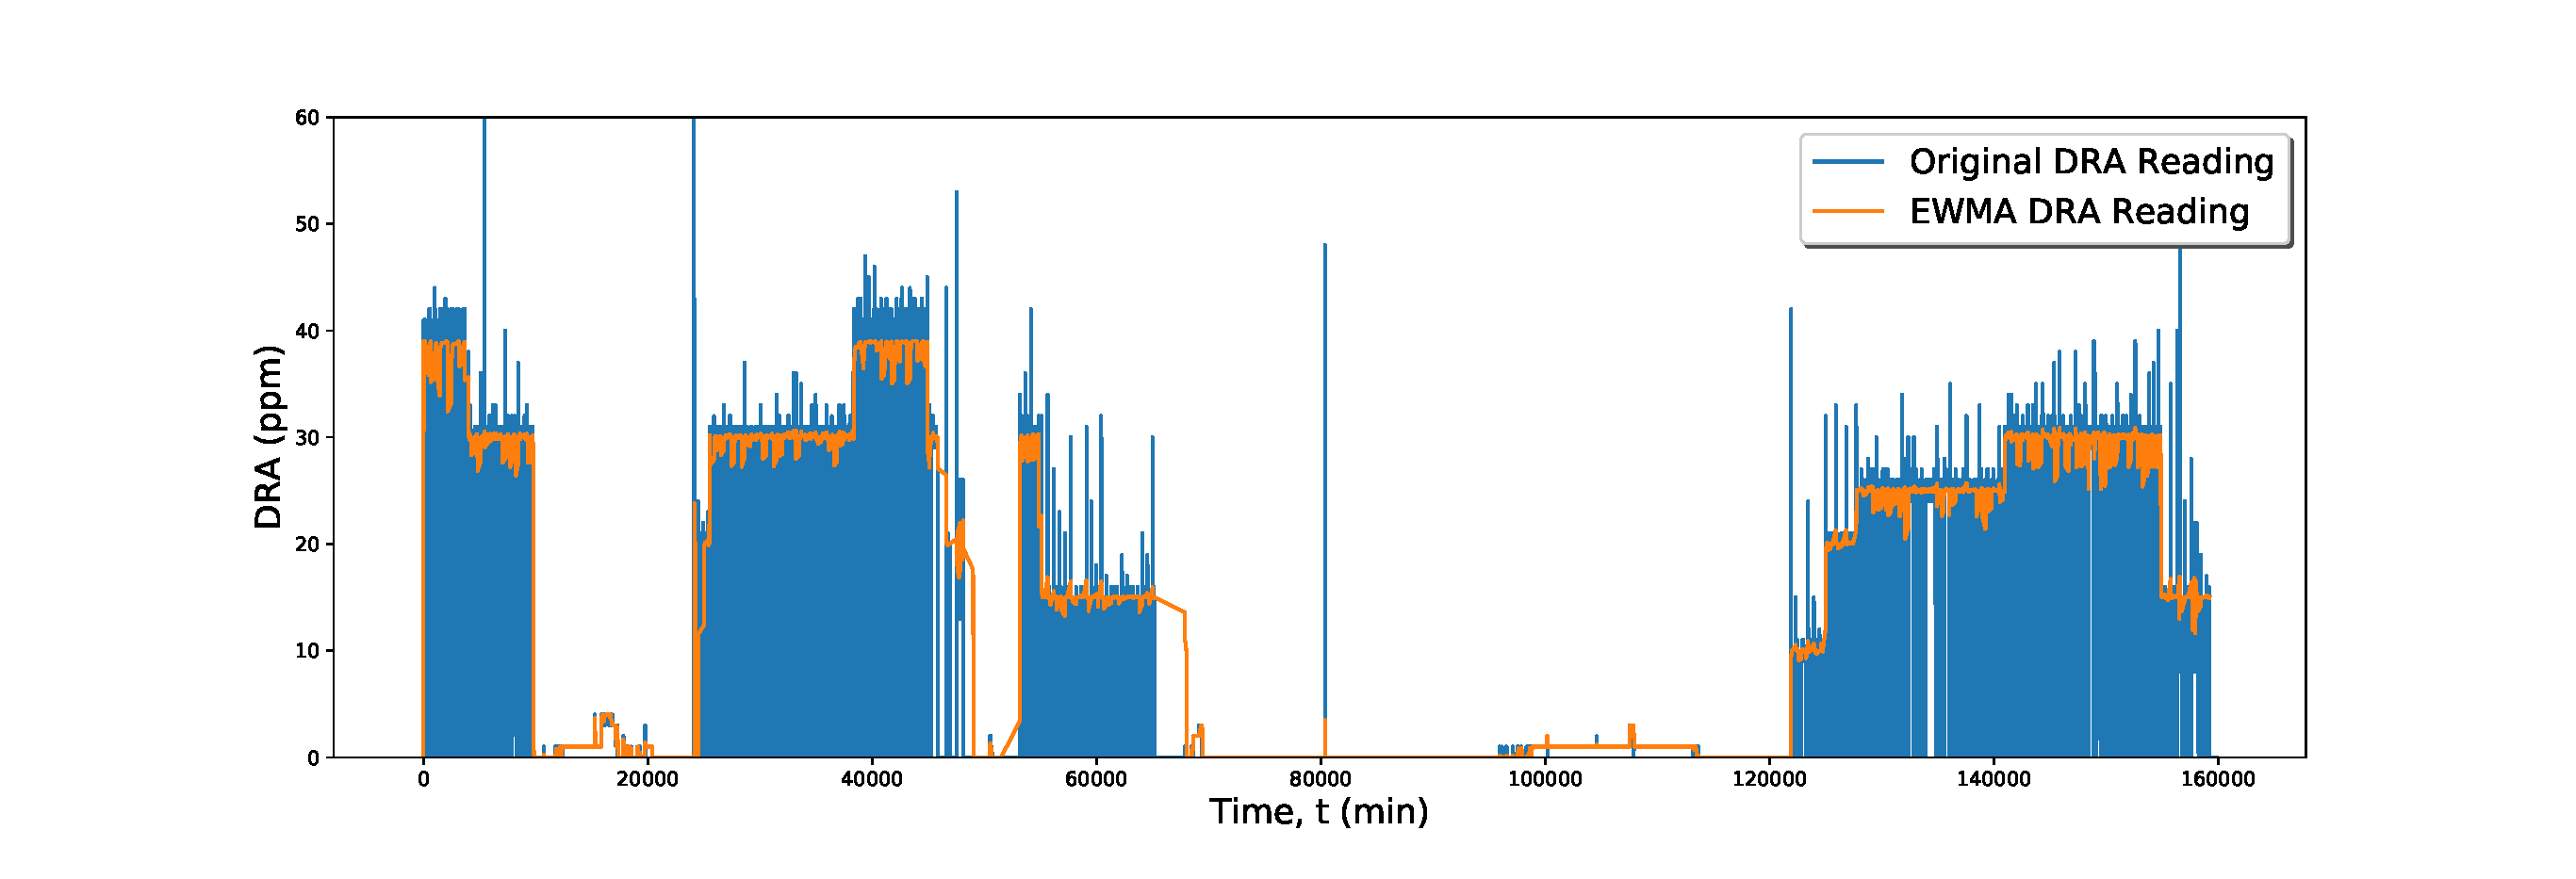
\includegraphics[width=\textwidth]{images/suncor/08CIGSweet.eps}
         \caption{Station B2 light DRA sensor reading.}
     \end{subfigure}
     \begin{subfigure}[b]{0.9\textwidth}
         \centering
         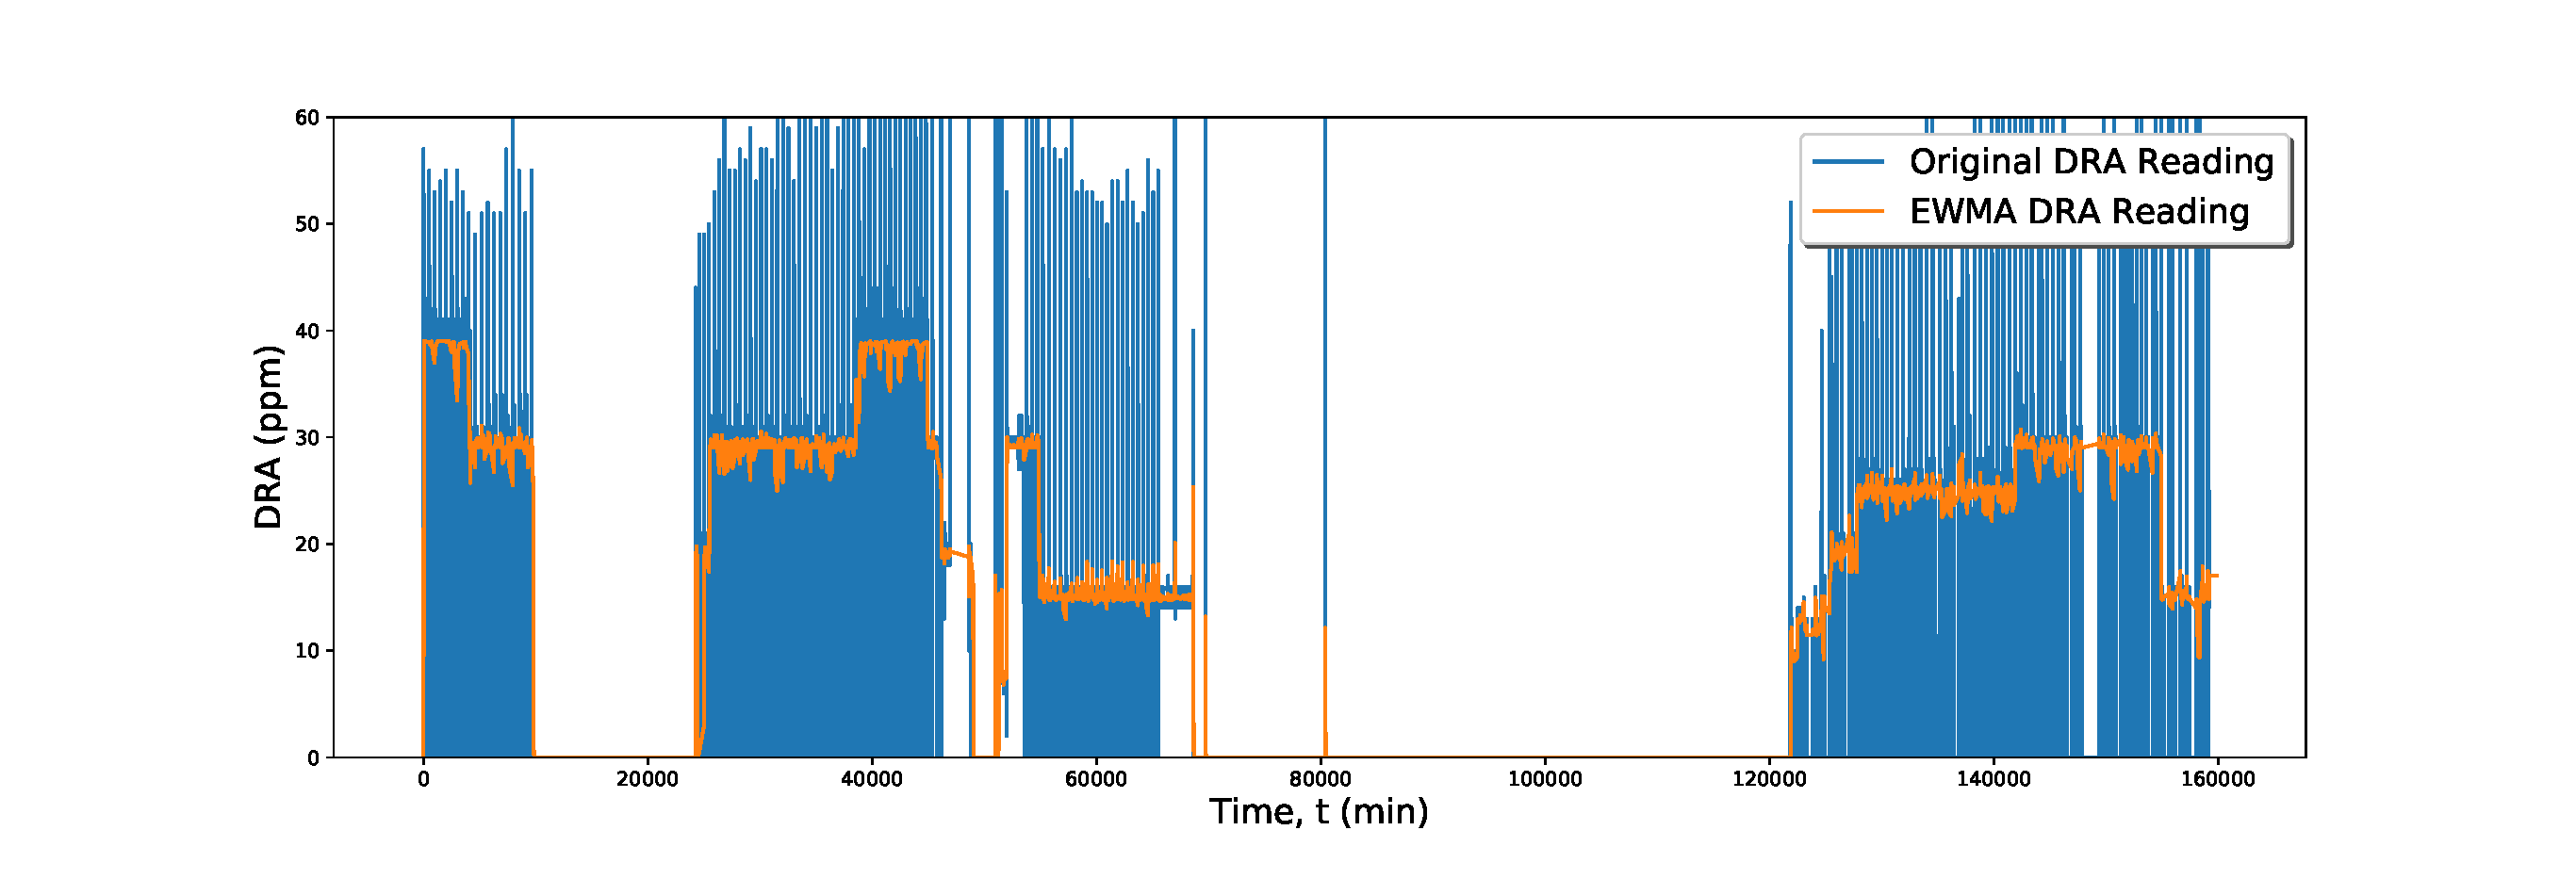
\includegraphics[width=\textwidth]{images/suncor/08AultSour.eps}
         \caption{Station B3 heavy DRA sensor reading.}
     \end{subfigure}
     \begin{subfigure}[b]{0.9\textwidth}
         \centering
         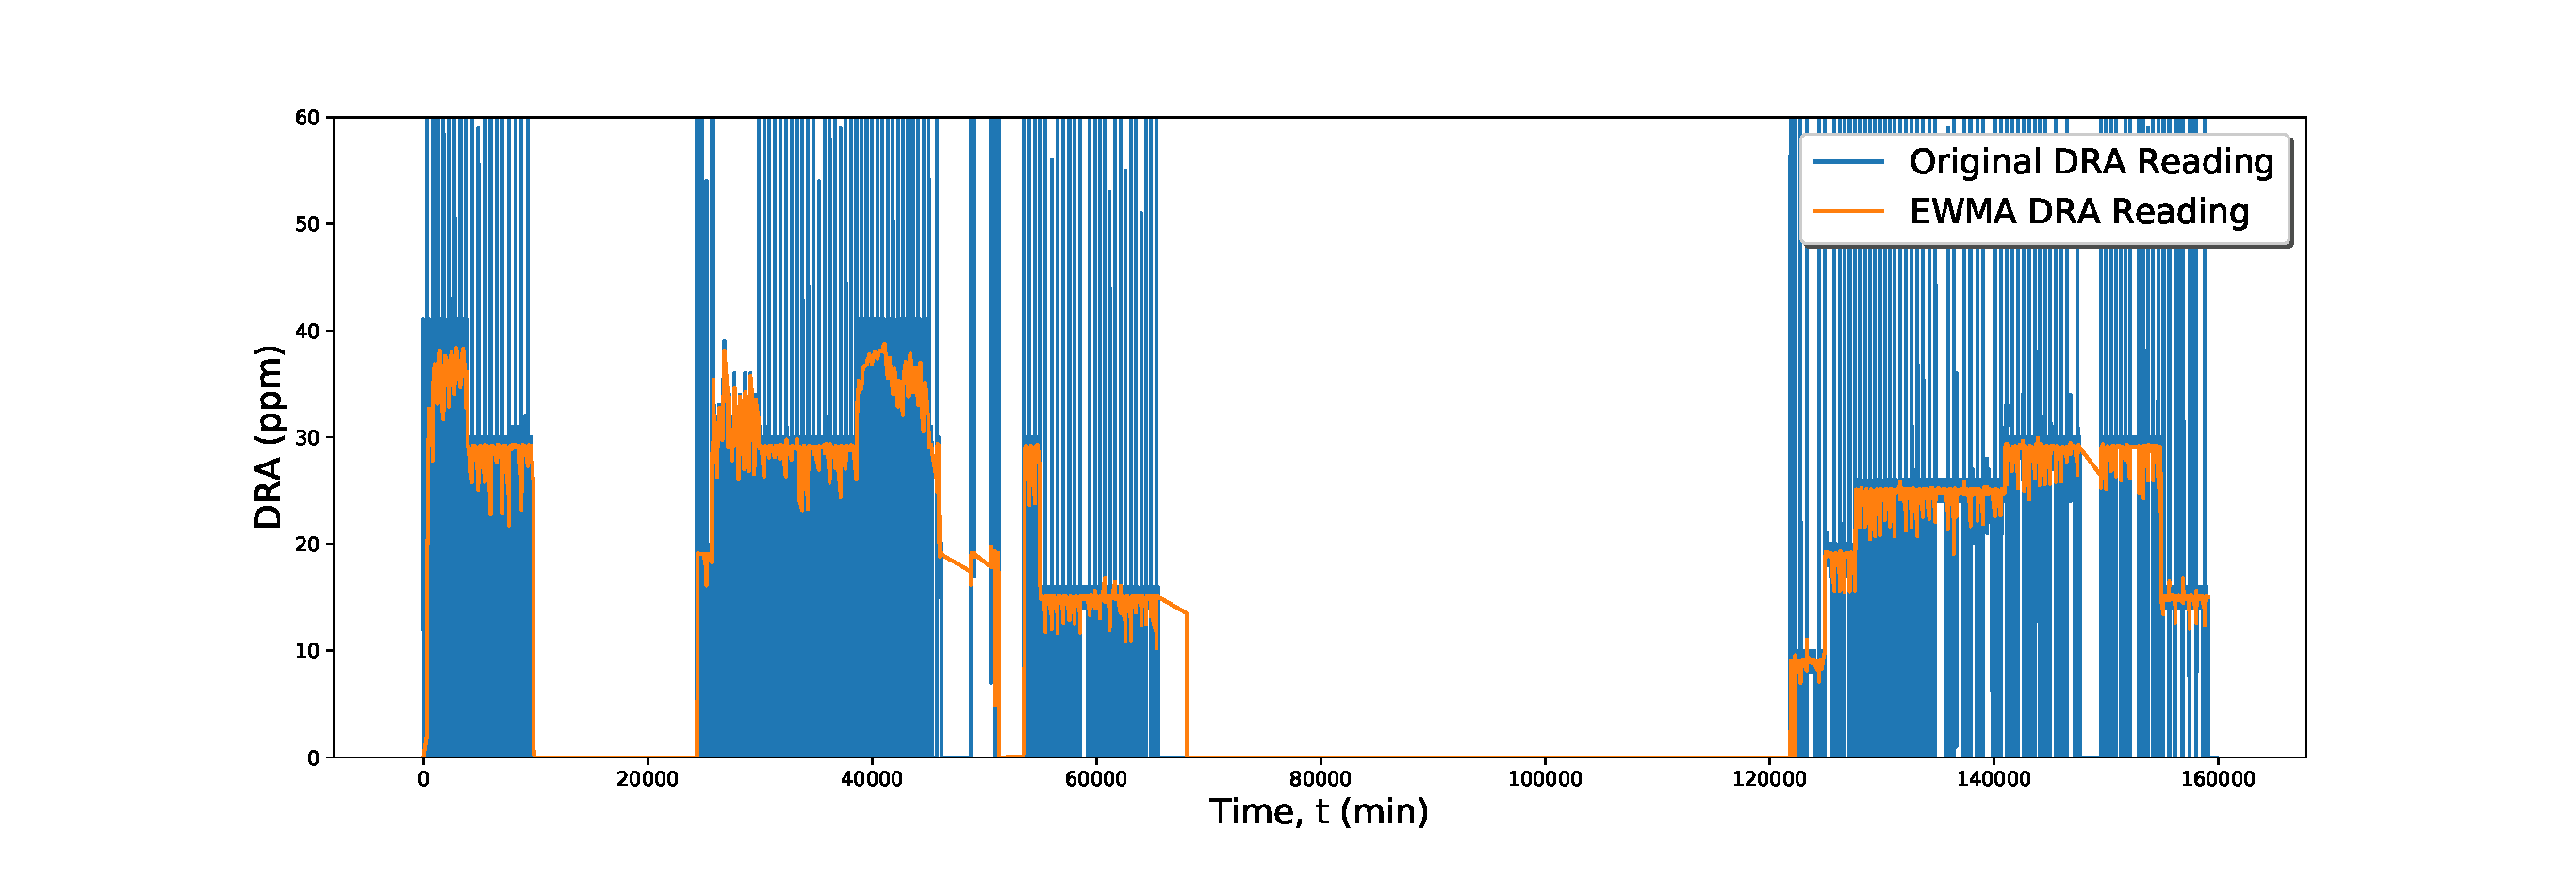
\includegraphics[width=\textwidth]{images/suncor/08AultSweet.eps}
         \caption{Station B2 light DRA sensor reading.}
     \end{subfigure}
        \caption{Pre- and post-processed DRA sensor readings.}
        \label{fig:02DRA}
\end{figure}

To conclude the data pre-processing procedure, the process operators were consulted with to identify any "special" considerations that should be included into the ML models.  Here, the operators stated that the density reading is unreliable and is only used to identify the crude type at each station. From this information, all density readings were feature engineered into binary readings where "1" represented light crude and "0" represented heavy crude to reflect the physical purpose of the reading.

Exploratory data analysis was then performed on the processed data to gain additional insight. In Figure \ref{fig:02KDE}, a kernel density estimation was applied to the pipeline outlet flow rate to identify its distribution as shown.  It can be seen that the flow rate follows a bi-modal distribution and most likely corresponds to two different operating regimes. To enhance ML model performance, the two modes were segregated using DBSCAN.  Here, DBSCAN was selected due to its scalability to big data and ability to identify outliers. The hyper parameters, $\epsilon$ and $min \; points$, for DBSCAN were 1.13 and 10,000, respectively.

\begin{figure}[h]
    \centering
    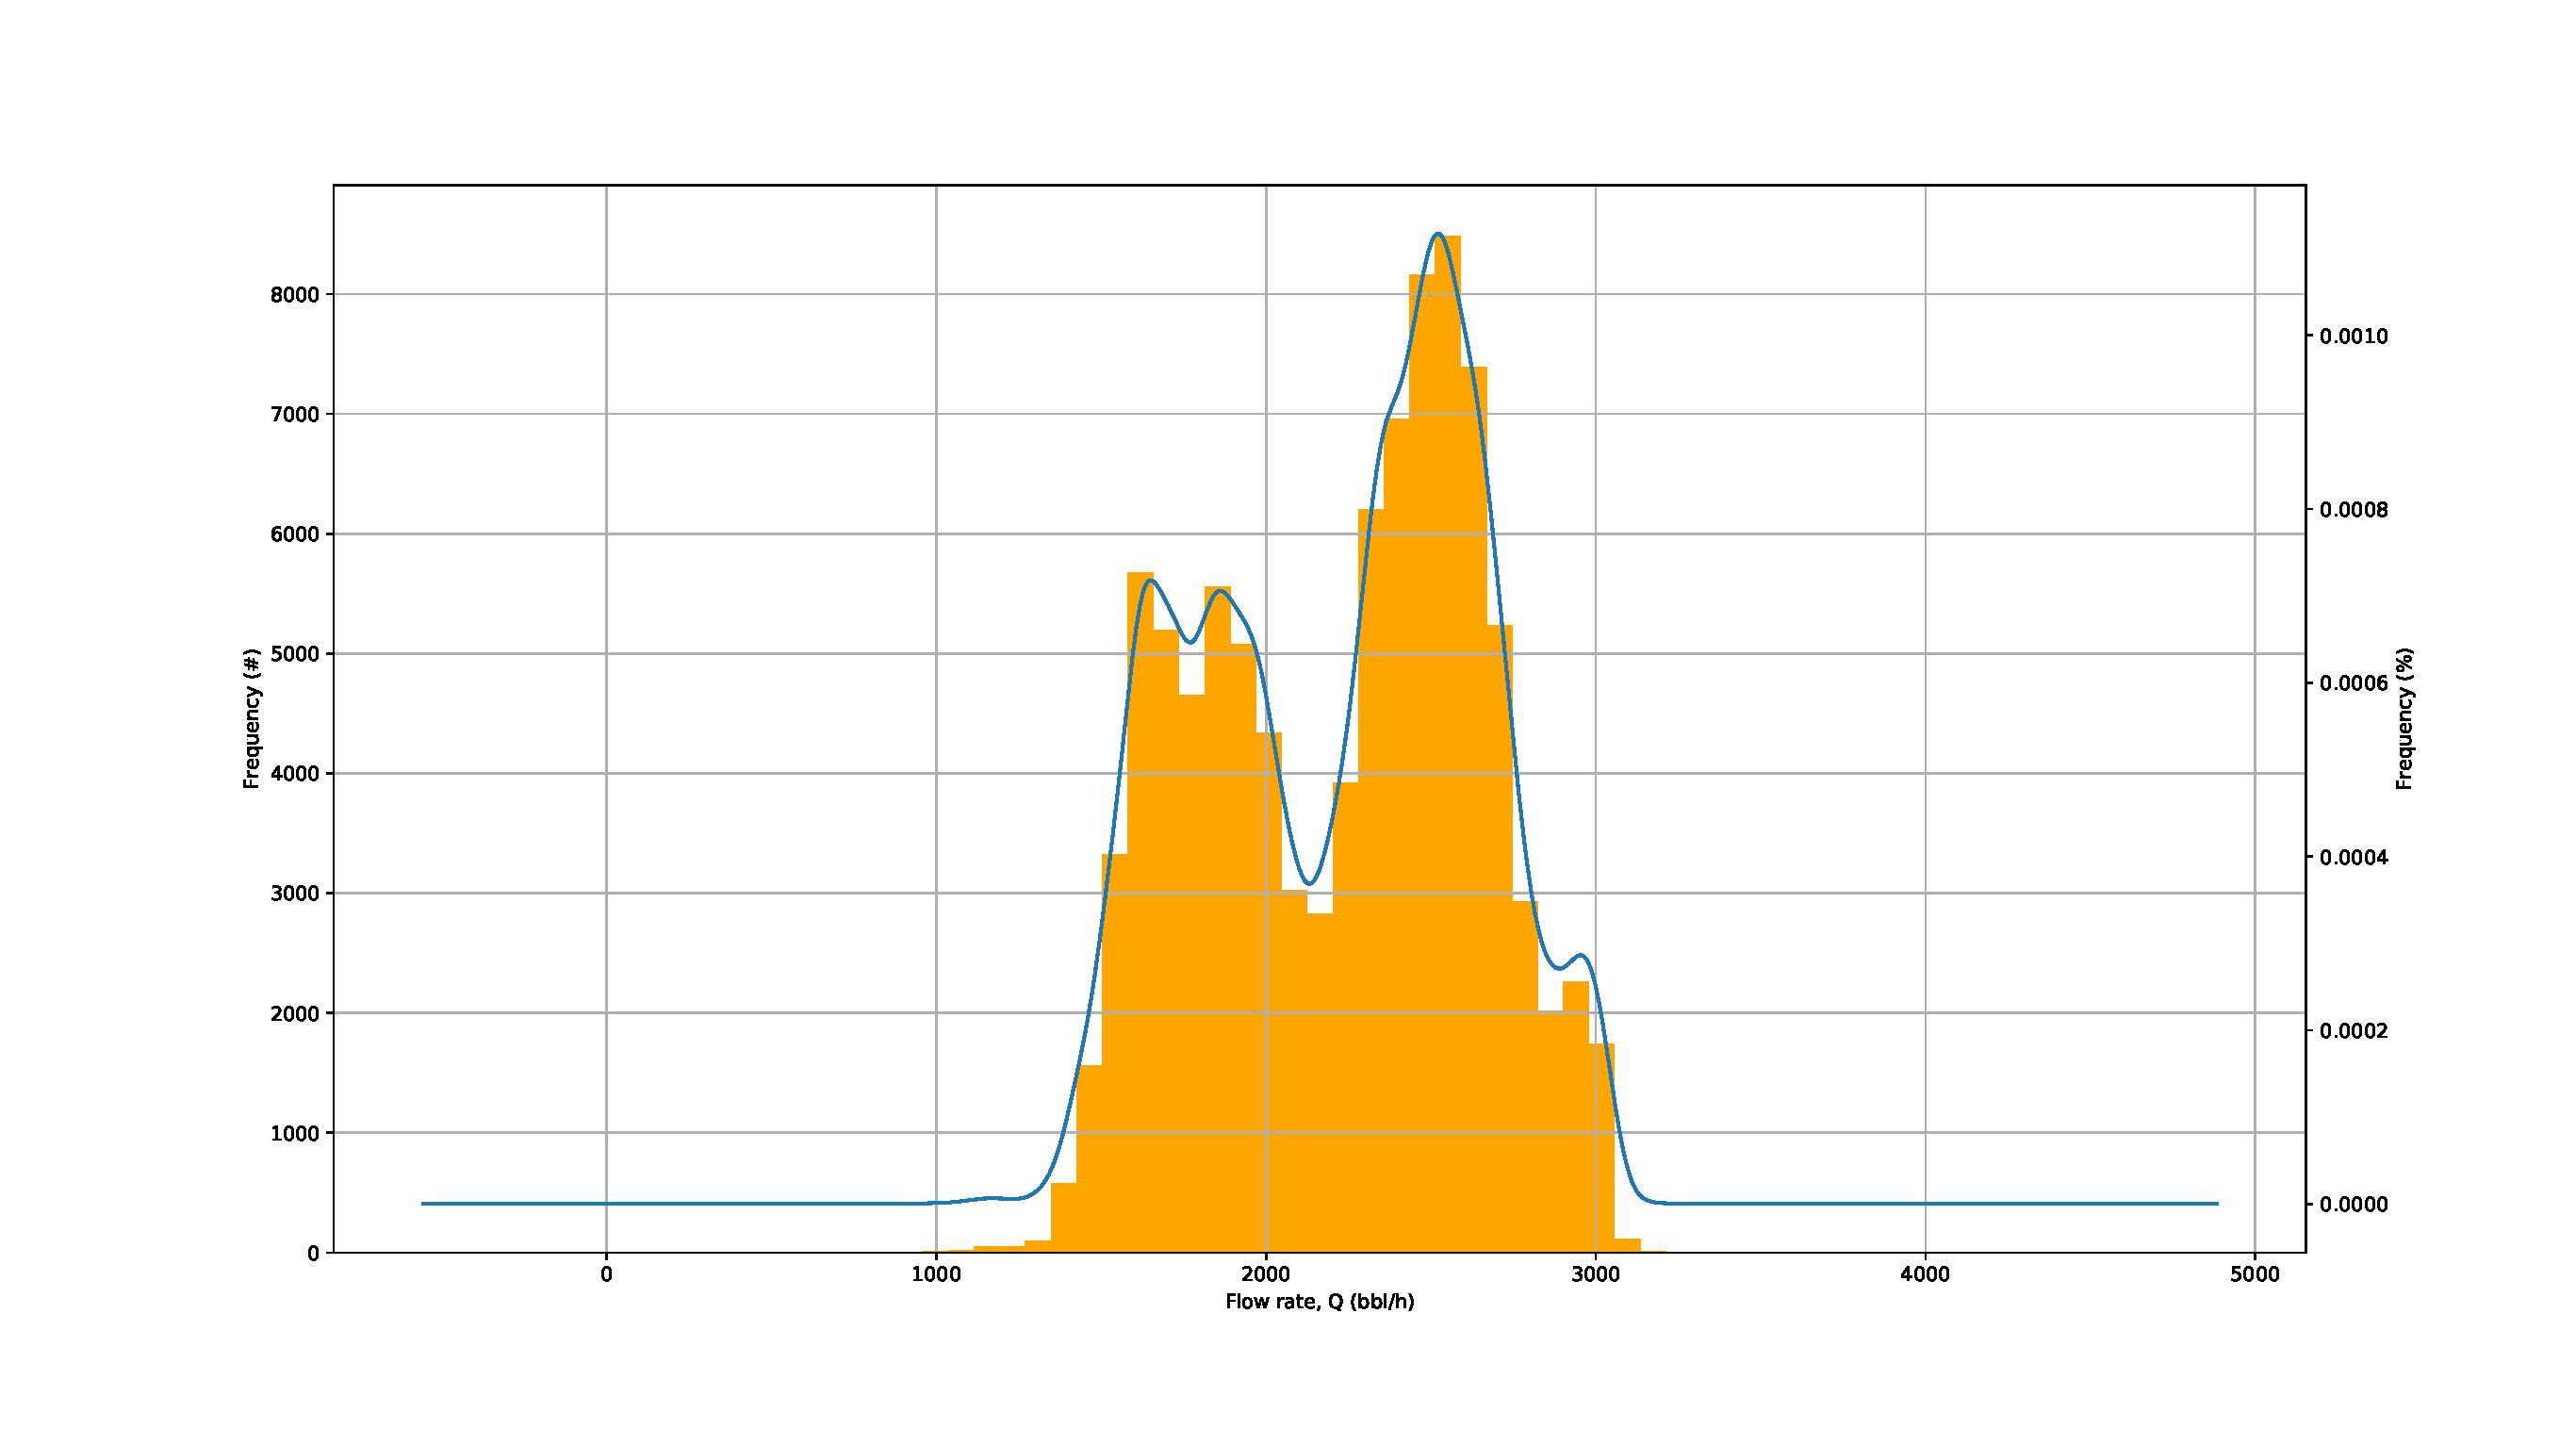
\includegraphics[width=\textwidth]{images/suncor/08Flowrate_KDE.eps}
    \caption{Flow rate distribution of the pre-processed data set.}
    \label{fig:02KDE}
\end{figure}

The segregated distributions created from DBSCAN and the average characteristics of each cluster are shown in Figures \ref{fig:02DBSCAN} and \ref{fig:02DBSCANV}, respectively.  Evidently from Figure \ref{fig:02DBSCANV}, the operation of equipment were vastly different in the two operating regimes.  More specifically, cluster 2 used almost no DRA, and used Station B3 Pump 1 and Station B1 VFD exclusively.  In cluster 1, all equipment were used with exception of Station B3 Pump 1.  From this information, two ML models can be created to cater to each cluster.

\begin{figure}[h]
    \centering
    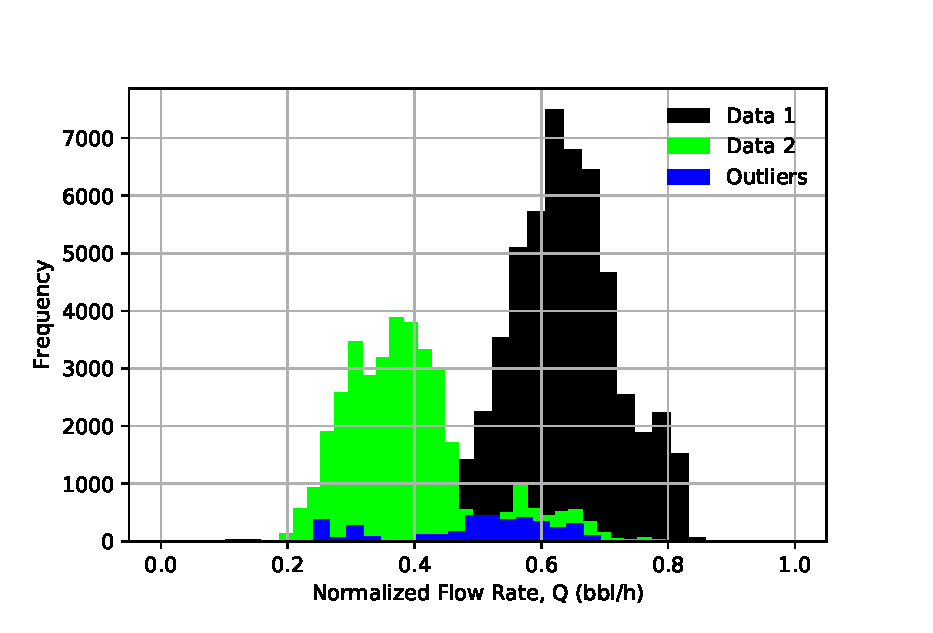
\includegraphics[scale=0.8]{images/suncor/08DBSCAN.eps}
    \caption{Clusters identified after applying the density-based scan.}
    \label{fig:02DBSCAN}
\end{figure}

\begin{figure}[h]
    \centering
    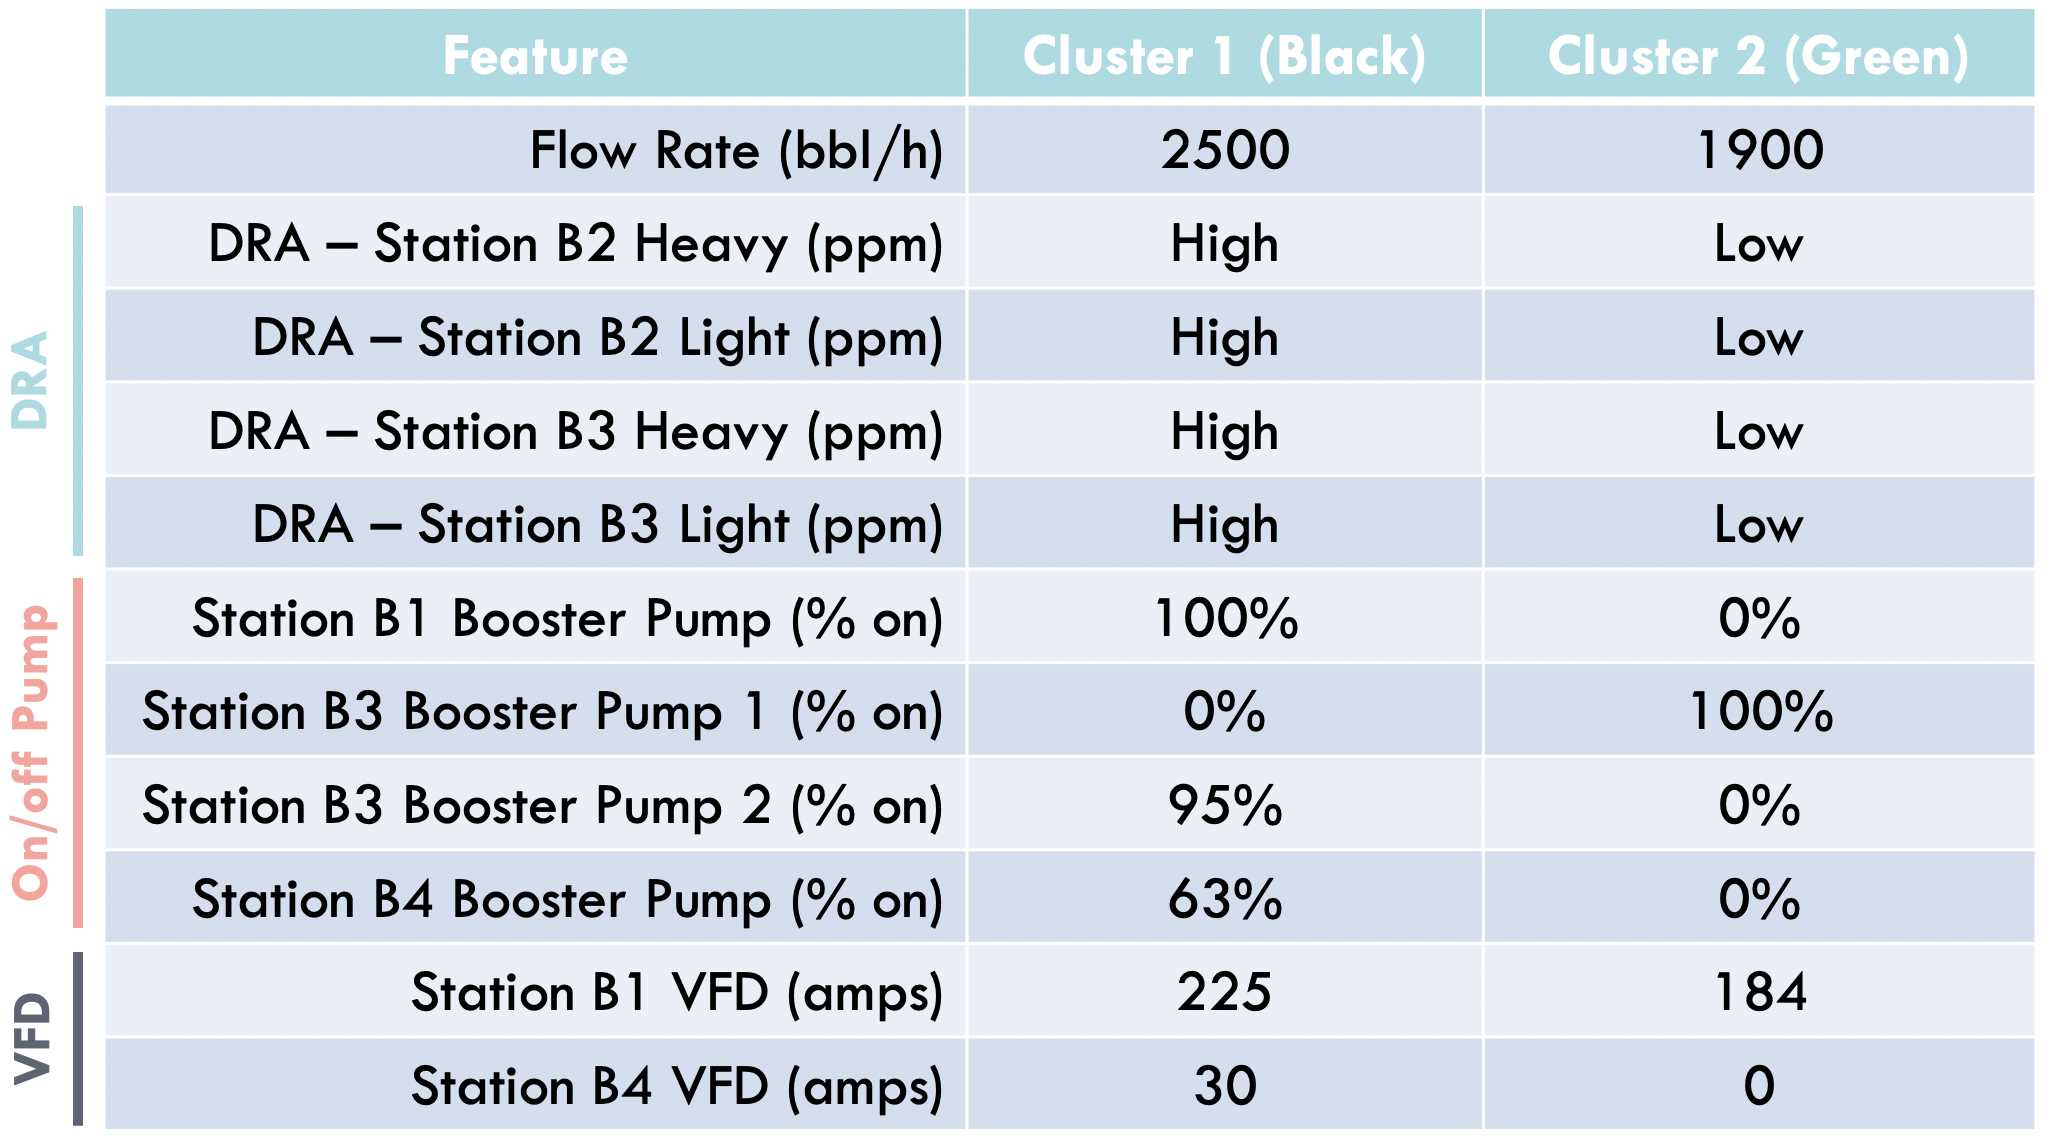
\includegraphics[width=0.8\textwidth]{images/suncor/08AvgChar.jpeg}
    \caption{Average operating variables for the two operating conditions.}
    \label{fig:02DBSCANV}
\end{figure}

\subsection{Machine Learning Predictions}

The following models were implemented to predict for the pipeline outlet flow rate: linear models, polynomial models, neural network models, and LPV models.  Ultimately, the LPV model reigned supreme due to its interpretability, consistent results, simple model structure. The performance and hyper parameters of each model are shown below.  During model identification, the data sets were divided into three sections: training, validation and testing.  Table \ref{tab:02datapart} shows the purpose of each data section.
\begin{table}[h]
    \centering
    {\setstretch{1.2}
    \begin{tabular}{ c | c | p{9cm}}
                            & \% of Data        &  Description \\
        \hline
        Training            &  90\%             
        &  Identify the ML model        \\
        
        Validation          &  5\%              
        &  Tune ML model performance on unseen data         \\
        
        Testing             &  5\%             
        &  Test ML model performance on proxy live data       \\             
    \end{tabular}}
    \caption{Description of each data partition.}
    \label{tab:02datapart}
\end{table}

\subsubsection{Linear Models}
Linear models pertain the simplest model structure and will serve as a benchmark for other models.  The hyper parameters and performance metrics of the model are shown in Table \ref{tab:02LinearHP} and \ref{tab:02LinearPE}, respectively. The model's performance on the validation and test data are shown in Figures \ref{fig:02LSValidation} and \ref{fig:02LSTest}. From \ref{tab:02LinearPE}, the model MAE and RMSE increased 4\% and 6\% on the testing data, respectively.  $R^2$ on the test data significantly reduced.  However, the trends from Figure \ref{fig:02LSTest} does not exhibit any significant inaccuracies. 

\begin{table}[h]
    \centering
    {\setstretch{1.2}
    \begin{tabular}{ c | c}
        Hyper Parameter                  &  Value       \\
        \hline
        Epochs                           &  800      \\
        Minibatch size                   &  8192     \\
        Learning rate, $\alpha$          &  0.001    \\
        Regularization, $\lambda$          &  0.001  \\
    \end{tabular}}
    \caption{Hyper parameters for linear regression.}
    \label{tab:02LinearHP}
\end{table}
\begin{table}[h]
    \centering
    {\setstretch{1.2}
    \begin{tabular}{ c | c | c | c}
                             &  Training data    &  Validation data   &    Test data      \\
        \hline
        MAE                  &  98               &    98              &  102     \\
        RMSE                 &  127              &   127              &  135    \\ 
        $R^2$                &  0.91             &   0.91             &  0.70   \\
    \end{tabular}}
    \caption{Performance assessment for the linear regression.}
    \label{tab:02LinearPE}
\end{table}

\begin{figure}[h]
     \centering
     \begin{subfigure}[b]{0.48\textwidth}
         \centering
         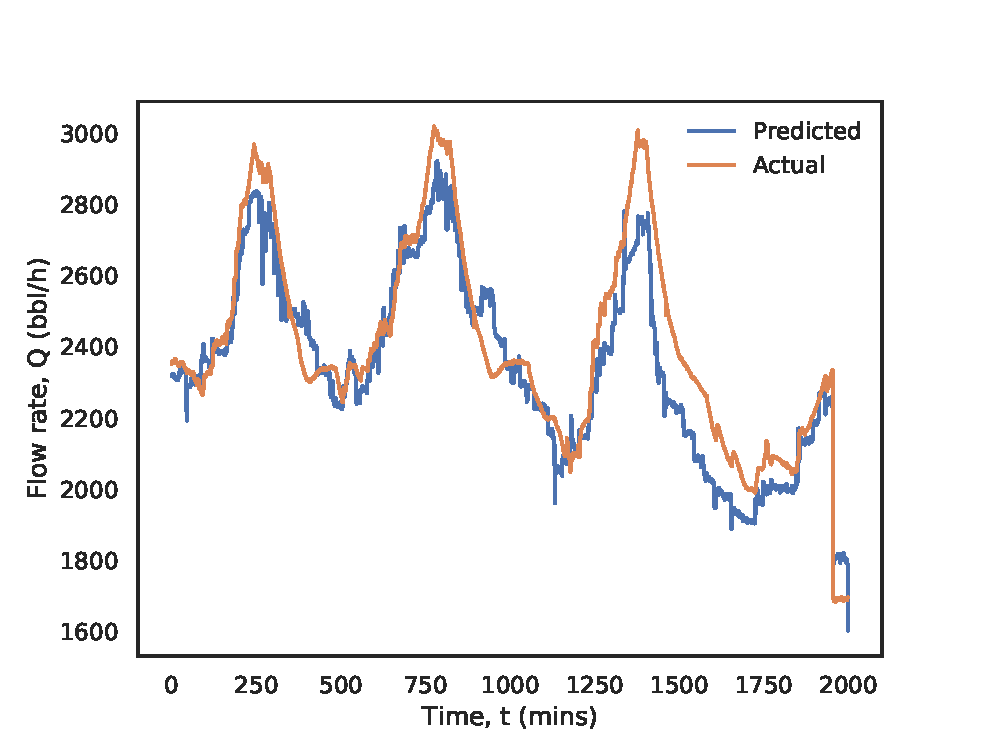
\includegraphics[width=\textwidth]{images/suncor/08ls_validation.eps}
         \caption{Predicted vs. actual flow rate for the validation data set.}
         \label{fig:02LSValidation}
     \end{subfigure}
     \hfill
     \begin{subfigure}[b]{0.48\textwidth}
         \centering
         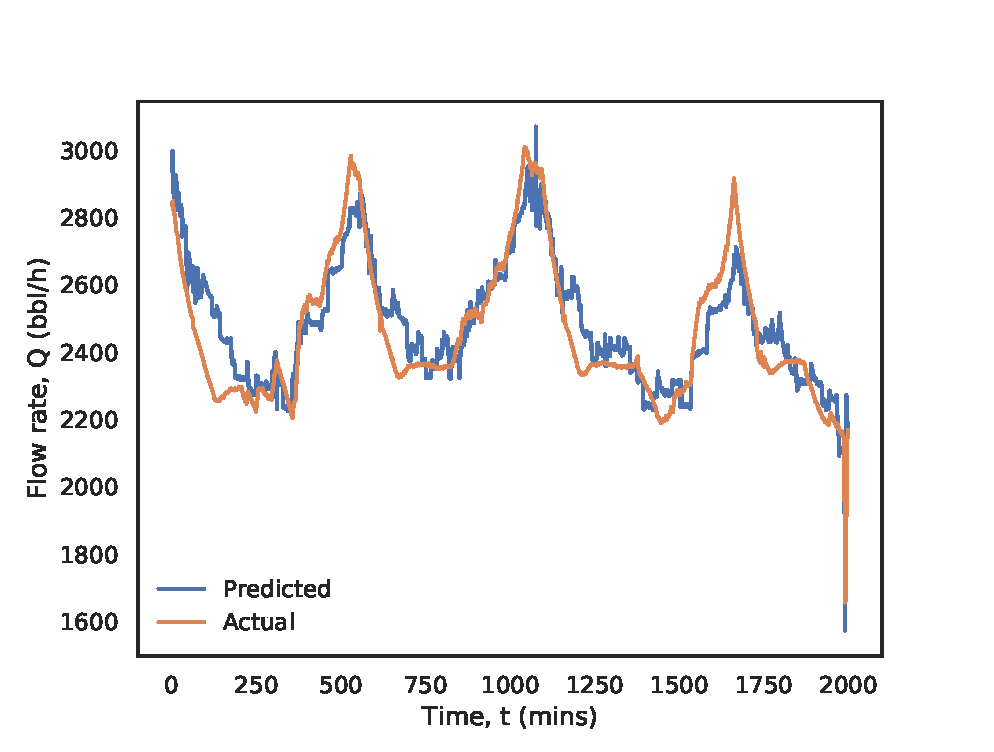
\includegraphics[width=\textwidth]{images/suncor/08ls_test.eps}
         \caption{Predicted vs. actual flow rate for the test data set.}
         \label{fig:02LSTest}
     \end{subfigure}
     \caption{Linear regression validation and test plots.}
        \label{fig:02LSPlots}
\end{figure}

\subsubsection{Polynomial Models}
Non-linear models were used to further enhance predictive capabilities.  Two exponential models were applied: quadratic and square root.  The hyper parameters and performance metrics of the exponential models are shown in Tables \ref{tab:02ExponentialHP} and \ref{tab:02ExponentialHP}, respectively. The model performances on the validation and test data sets is shown in Figure \ref{fig:02PolynomialPlots}. Compared to the benchmark model, the MAE and RMSE decreased by up to 13\% and 15\% on the test data set. Moreover, the model performance does not deteriorate when applied on the test data set. 

\begin{table}[h]
    \centering
    {\setstretch{1.2}
    \begin{tabular}{ c | c | c}
        Hyper Parameter                  &  Quadratic   & Square root       \\
        \hline
        Epochs                           &  1000    & 1000  \\
        Minibatch size                   &  8192    & 8192    \\
        Learning rate, $\alpha$          &  0.001   & 0.001  \\
        Regularization, $\lambda$          &  0.001 & 0.001 \\
    \end{tabular}}
    \caption{Hyper parameters for exponential regression.}
    \label{tab:02ExponentialHP}
\end{table}

\begin{table}[h]
    \centering
    {\setstretch{1.2}
    \begin{tabular}{c|c|c|c|c|c|c|}
      & \multicolumn{2}{c|}{Training data} & \multicolumn{2}{c|}{Validation data} & \multicolumn{2}{c|}{Test data} \\ \cline{2-7} 
      & Quad             & Sqrt            & \multicolumn{1}{c|}{Quad}   & Sqrt   & Quad           & Sqrt          \\ \hline
    MAE   & 92               & 89              & 92                          & 89     & 89             & 91            \\
    RMSE  & 121              & 118             & \multicolumn{1}{c|}{121}    & 117    & 120            & 115           \\
    \end{tabular}}
    \caption{Performance assessment for the quad. and sqrt. model.}
    \label{tab:02ExponentialPE}
\end{table}

\begin{figure}[h]
     \centering
     \begin{subfigure}[b]{0.45\textwidth}
         \centering
         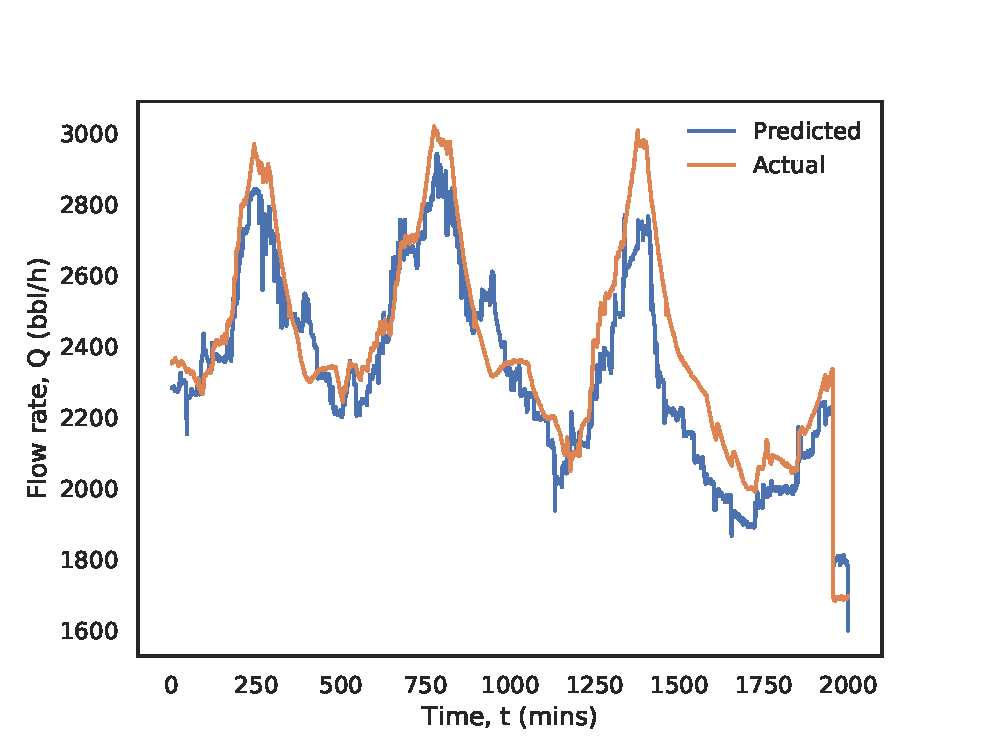
\includegraphics[width=\textwidth]{images/suncor/08quad_validation.eps}
         \caption{Predicted vs. actual flow rate for validation data using the quad. model.}
         \label{fig:02quad_validation}
     \end{subfigure}
     \begin{subfigure}[b]{0.45\textwidth}
         \centering
         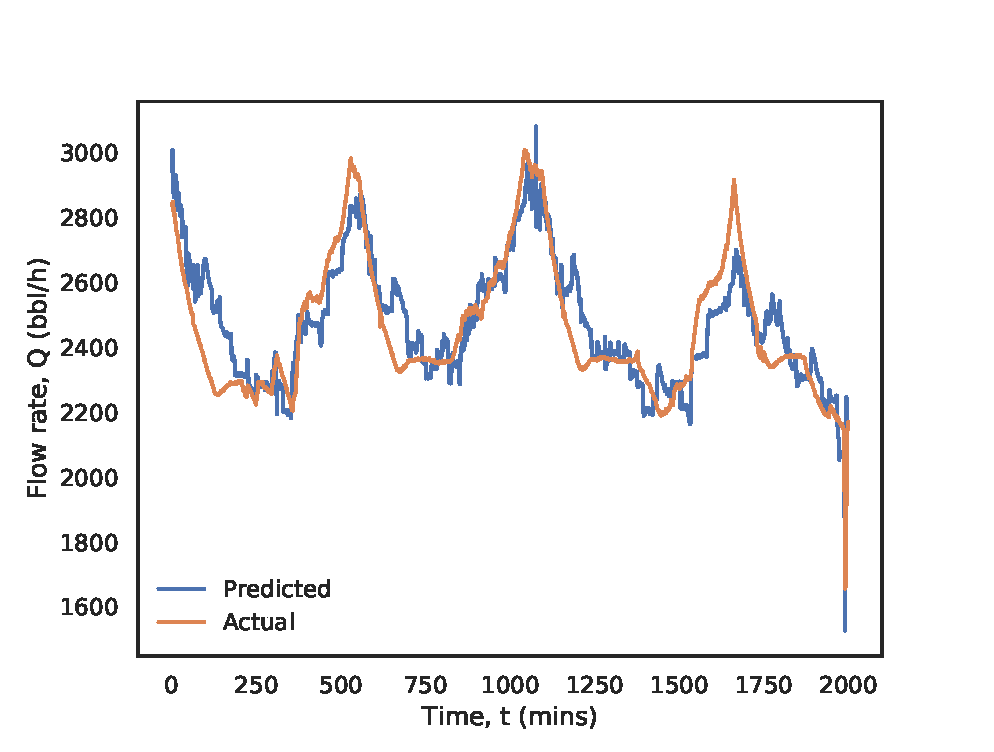
\includegraphics[width=\textwidth]{images/suncor/08quad_test.eps}
         \caption{Predicted vs. actual flow rate for the test data using the quadratic model.}
         \label{fig:02quad_test}
     \end{subfigure}
     \begin{subfigure}[b]{0.45\textwidth}
         \centering
         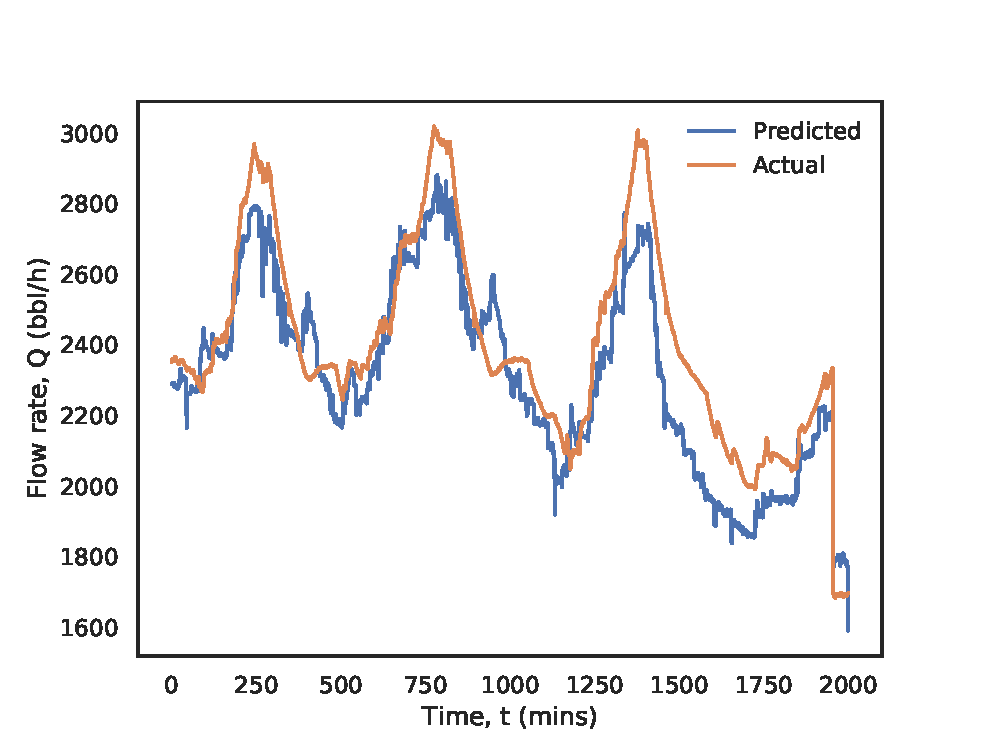
\includegraphics[width=\textwidth]{images/suncor/08sqrt_validation.eps}
         \caption{Predicted vs. actual flow rate for the validation data using the sqrt. model.}
         \label{fig:02sqrt_validation}
     \end{subfigure}
     \begin{subfigure}[b]{0.45\textwidth}
         \centering
         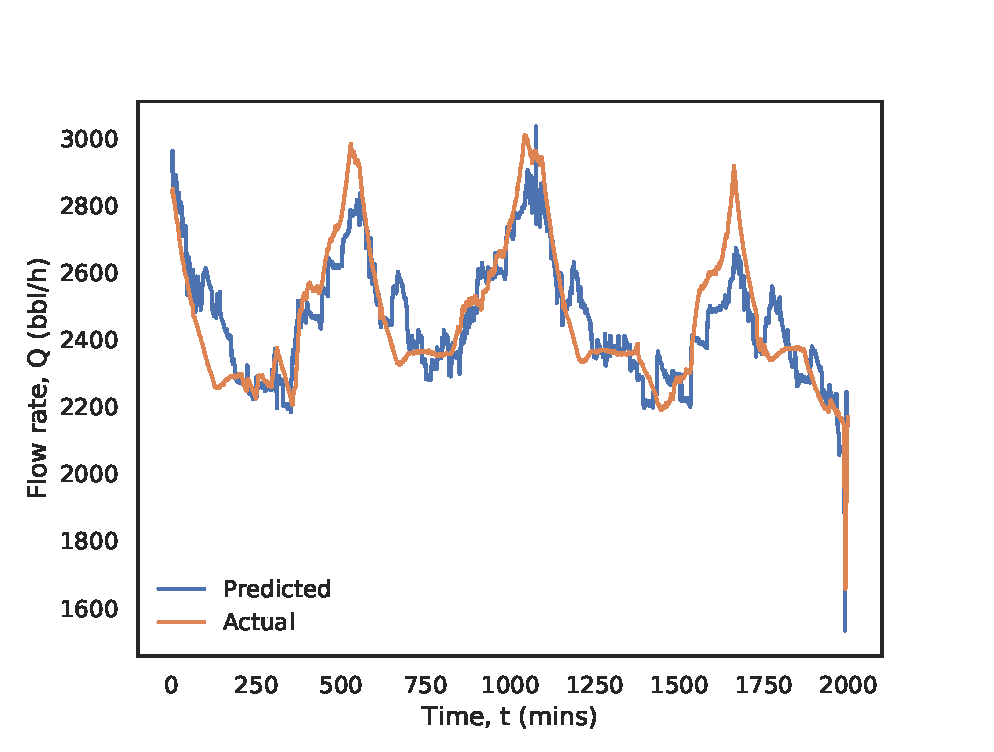
\includegraphics[width=\textwidth]{images/suncor/08sqrt_test.eps}
         \caption{Predicted vs. actual flow rate for the test data using the sqrt. model.}
         \label{fig:02sqrt_test}
     \end{subfigure}
        \caption{Polynomial regression validation and test plots.}
        \label{fig:02PolynomialPlots}
\end{figure}

\subsubsection{Neural Network Models}
Neural networks and deep learning were the most advanced models to be applied to this prediction task.  Here, three different neural networks with varying sizes were trained and their performances evaluated. 

Tables \ref{tab:02NNHP} and \ref{tab:02NNPE} show the hyper parameters and performance metrics of the three neural networks.  Figure \ref{fig:02NNPlots} shows the neural networks' performance on the validation and test data sets.  From Table \ref{tab:02NNPE}, it is clear that the training and validation error decreased as the neural network increased in size; however, the errors increased significantly on the test data. This was caused by the test data being different than the training data.  In this particular case, the test data was collected in the summer months where temperatures increased by up to $\ang{10}$ C compared to the training data.  Because of the complexity and parameterization of neural network models, data even slightly different from the training data can have a significant impact on accuracy.  Smaller, simpler, more regularized neural network models could be used to avoid this behaviour. Indeed, it can be seen that the test data error increased as the size of the network increased. Another disadvantage of neural networks are its lack of interpretability.  Investigating the effects of each regressor in this highly non-linear model is nearly impossible; hence, neural networks are black box models and might be undesirable for safety critical systems.
\begin{table}[h]
    \centering
    {\setstretch{1.2}
    \begin{tabular}{ c | c | c | c}
        Hyper Parameter                            &  Small NN  &  Med. NN  & Large NN       \\
        \hline
        Epochs                                     &  700       & 1000      & 1200  \\
        Minibatch size                             &  8192      & 8192      & 8192  \\
        Learning rate, $\alpha$                    &  0.001     & 0.001     & 0.001 \\
        Regularization, $\lambda$                  &  0.001     & 0.003     & 0.005 \\
        Number of layers                           &  3         & 6         & 8     \\
        Neurons per layer                          &  20        & 30        & 40    \\
        Activation function for hidden layers      & ReLU       & ReLU      & ReLU  \\
        Activation function for hidden layers      & Linear     & Linear    & Linear \\
    \end{tabular}}
    \caption{Hyper parameters for the feed-forward neural network.}
    \label{tab:02NNHP}
\end{table}

\begin{table}[h]
\centering
{\setstretch{1.2}
\begin{tabular}{c|c|c|c|c|c|c|c|c|c|}
\multicolumn{1}{l|}{} & \multicolumn{3}{c|}{Training Data}                                               & \multicolumn{3}{c|}{Validation Data}                                             & \multicolumn{3}{c|}{Test Data}                                                   \\ \cline{2-10} 
\multicolumn{1}{l|}{} & \multicolumn{1}{c|}{Sm.} & \multicolumn{1}{c|}{Med.} & \multicolumn{1}{c|}{Lar.} & \multicolumn{1}{c|}{Sm.} & \multicolumn{1}{c|}{Med.} & \multicolumn{1}{c|}{Lar.} & \multicolumn{1}{c|}{Sm.} & \multicolumn{1}{c|}{Med.} & \multicolumn{1}{c|}{Lar.} \\ \hline
MAE                   & 48                       & 42                        & 38                        & 50                       & 45                        & 37                        & 87                       & 87                        & 91                        \\
RMSE                  & 66                       & 58                        & 57                        & 69                       & 61                        & 56                        & 107                      & 117                       & 118                       \\
\end{tabular}}
    \caption{Performance assessment of the neural network models.}
    \label{tab:02NNPE}
\end{table}

\begin{figure}[p]
     \centering
     \begin{subfigure}[b]{0.48\textwidth}
         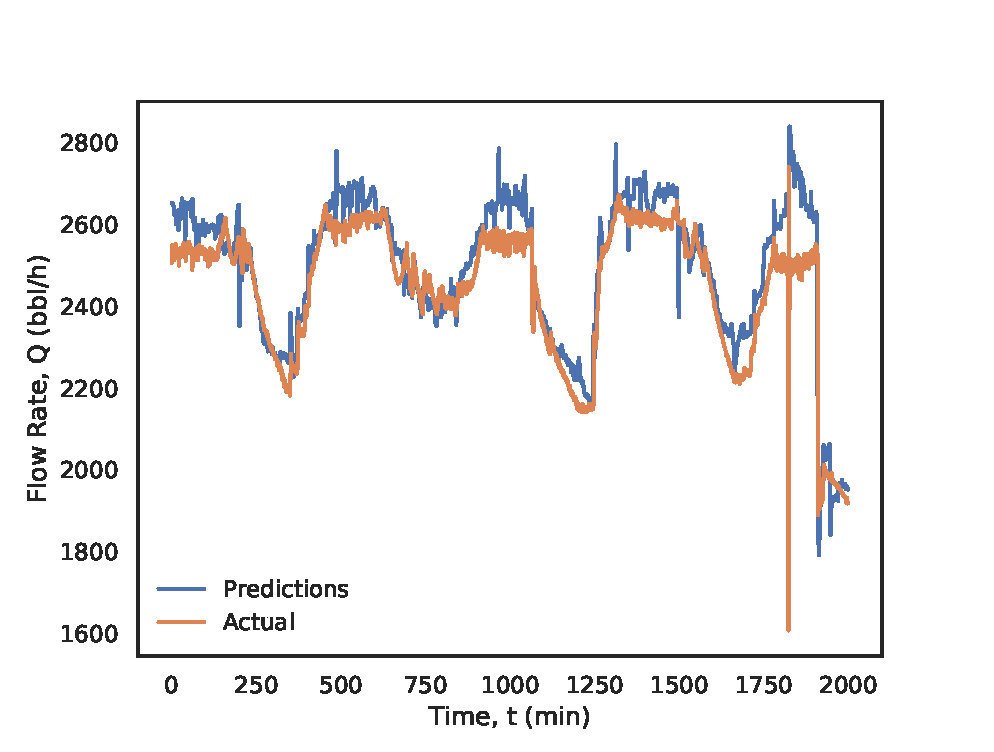
\includegraphics[width=\textwidth]{images/suncor/08smallnn_valid.eps}
         \caption{Validation data for the small neural net.}
         \label{fig:02smallnn_valid}
     \end{subfigure}
     \begin{subfigure}[b]{0.48\textwidth}
         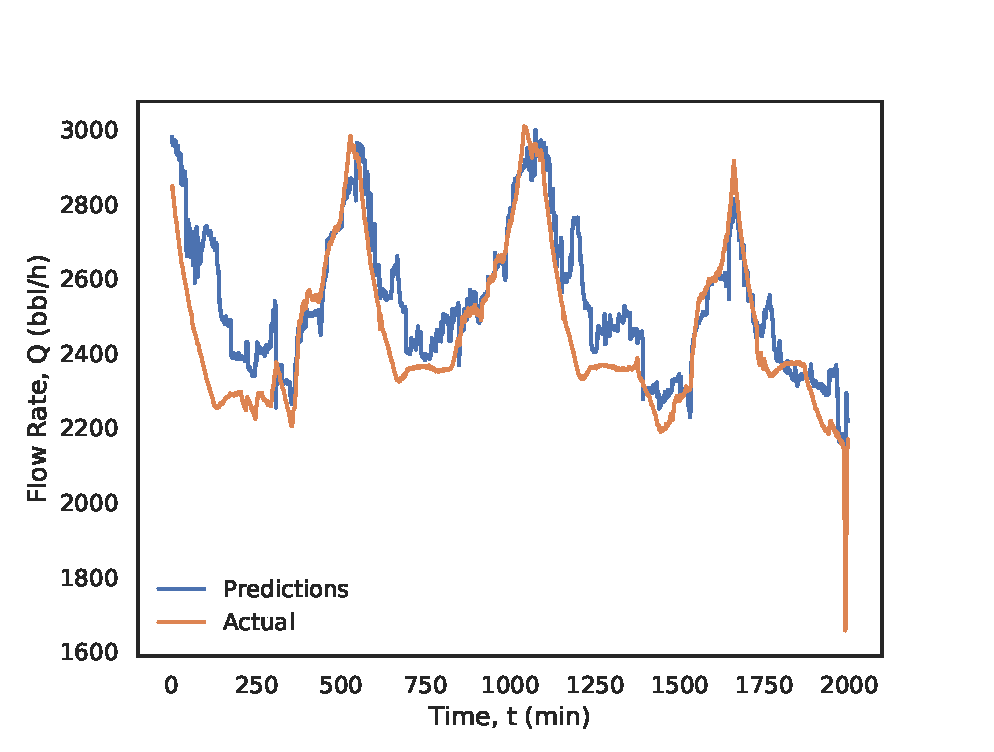
\includegraphics[width=\textwidth]{images/suncor/08smallnn_test.eps}
         \caption{Test data for the small neural net.}
         \label{fig:02smallnn_test}
     \end{subfigure}
     \begin{subfigure}[b]{0.48\textwidth}
         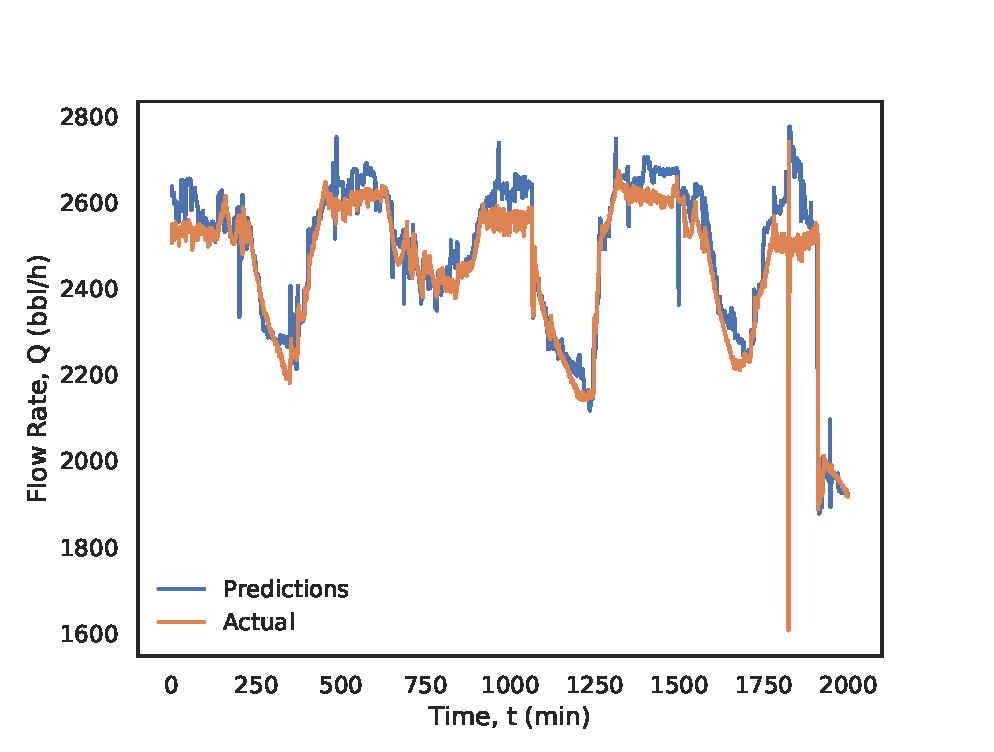
\includegraphics[width=\textwidth]{images/suncor/08mednn_valid.eps}
         \caption{Validation data for the med. neural net.}
         \label{fig:02mednn_valid}
     \end{subfigure}
     \begin{subfigure}[b]{0.48\textwidth}
         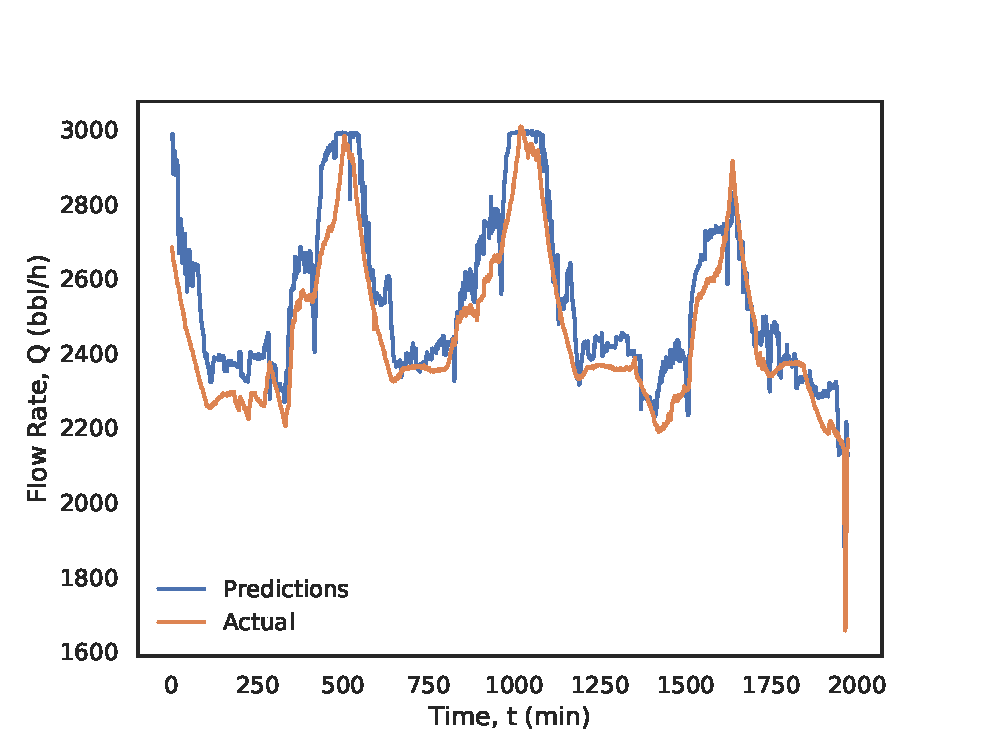
\includegraphics[width=\textwidth]{images/suncor/08mednn_test.eps}
         \caption{Test data for the med. neural net.}
         \label{fig:02mednn_test}
     \end{subfigure}
     \begin{subfigure}[b]{0.48\textwidth}
         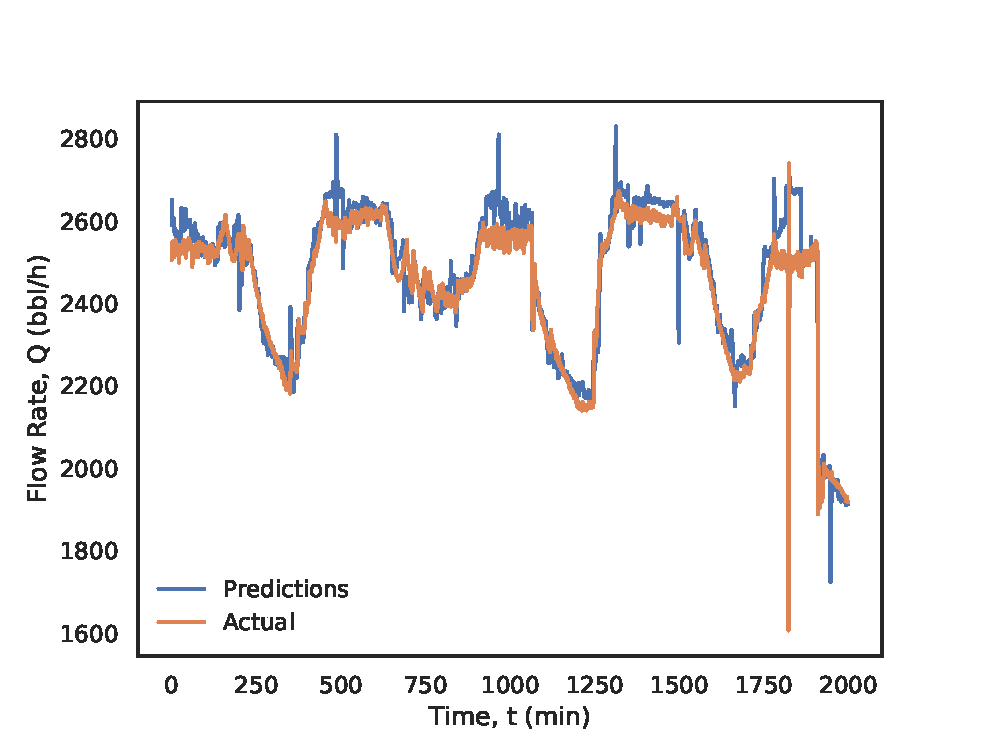
\includegraphics[width=\textwidth]{images/suncor/08largenn_valid.eps}
         \caption{Validation data for the large neural net.}
         \label{fig:02largenn_valid}
     \end{subfigure}
     \begin{subfigure}[b]{0.48\textwidth}
         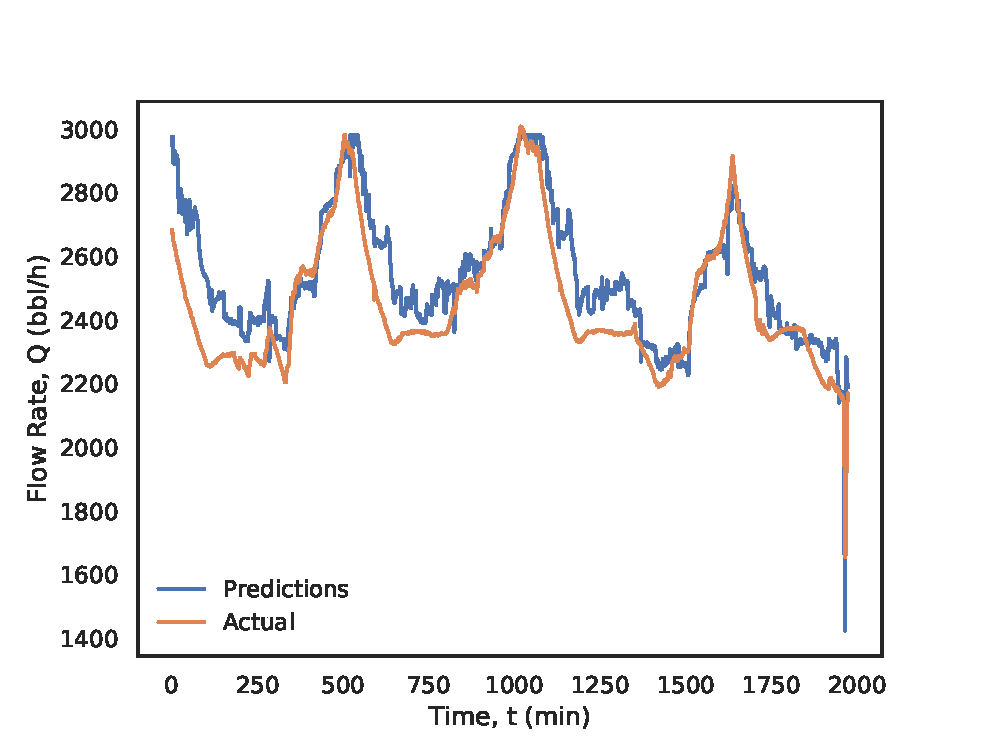
\includegraphics[width=\textwidth]{images/suncor/08largenn_test.eps}
         \caption{Test data for the large neural net.}
         \label{fig:02largenn_test}
     \end{subfigure}
        \caption{Predicted vs. actual flow rates for the feed-forward neural networks.}
        \label{fig:02NNPlots}
\end{figure}


\subsubsection{Linear Parameter-varying Models}
Linear parameter-varying models achieve the performance of non-linear models using a system of linear models.  Furthermore, the models are fully interpretable through its weights.  From the author's experience, this model structure is an ideal starting point for most industrial applications.  For this project, two linear model were identified; one for each cluster in Figure \ref{fig:02DBSCAN}.

The hyper parameters for each linear model is identical to the values shown in Table \ref{tab:02LinearHP}. Performance metrics of the two linear models are shown in Table \ref{tab:02LPVPE}.  The model performance on the validation and test data sets are shown in Figure \ref{fig:02LPVPlots}. Average MAE and RMSE of the LPV model is nearly identical to the square root models (the best non-linear model).  Moreover, the linear models are simpler and have unique regressors in each model.  For example, the linear model for cluster 2 is only a function of the Station B1 VFD current and the DRA ppms because all other inputs did not change in the data set.  Visually, the performance figures show low correlation; however, this is because the validation and test data sets were different compared to the previous models since the data set had to be decomposed.  Additionally, the flow rate in these new data sets contain higher noise compared to previous data and the y-axis range is also reduced, enhancing the noise. Ultimately, the performance metrics illustrate that the performance of the LPV model is nearly identical to the non-linear models and was the model of choice in this industrial application.

\begin{table}[h]
    \centering
    {\setstretch{1.2}
    \begin{tabular}{c|c|c|c|c|c|c|}
      & \multicolumn{2}{c|}{Training data} & \multicolumn{2}{c|}{Validation data} & \multicolumn{2}{c|}{Test data} \\ \cline{2-7} 
      & Cl. 1            & Cl. 2           & Cl. 1             & Cl. 2            & Cl. 1          & Cl. 2         \\ \hline
    MAE   & 90               & 66              & 90                & 67               & 96             & 85            \\
    RMSE  & 115              & 91              & 116               & 92               & 120            & 110           \\
    $R^2$ & 0.87             & 0.90            & 0.86              & 0.89             & 0.78           & 0.57         
    \end{tabular}}
    \caption{Performance assessment for clusters 1 and 2 regression models.}
    \label{tab:02LPVPE}
\end{table}

\begin{figure}[h]
    \centering
     \begin{subfigure}[b]{0.48\textwidth}
         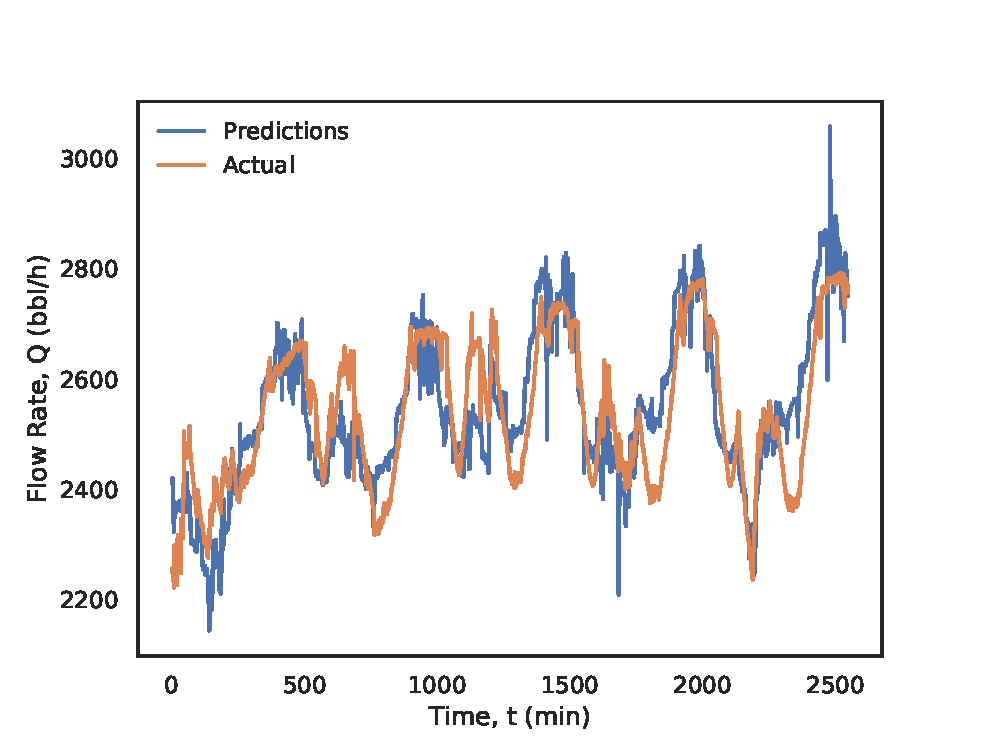
\includegraphics[width=\textwidth]{images/suncor/08cluster1_valid.eps}
         \caption{Validation data using model 1.}
         \label{fig:02cluster1_valid}
     \end{subfigure}
     \begin{subfigure}[b]{0.48\textwidth}
         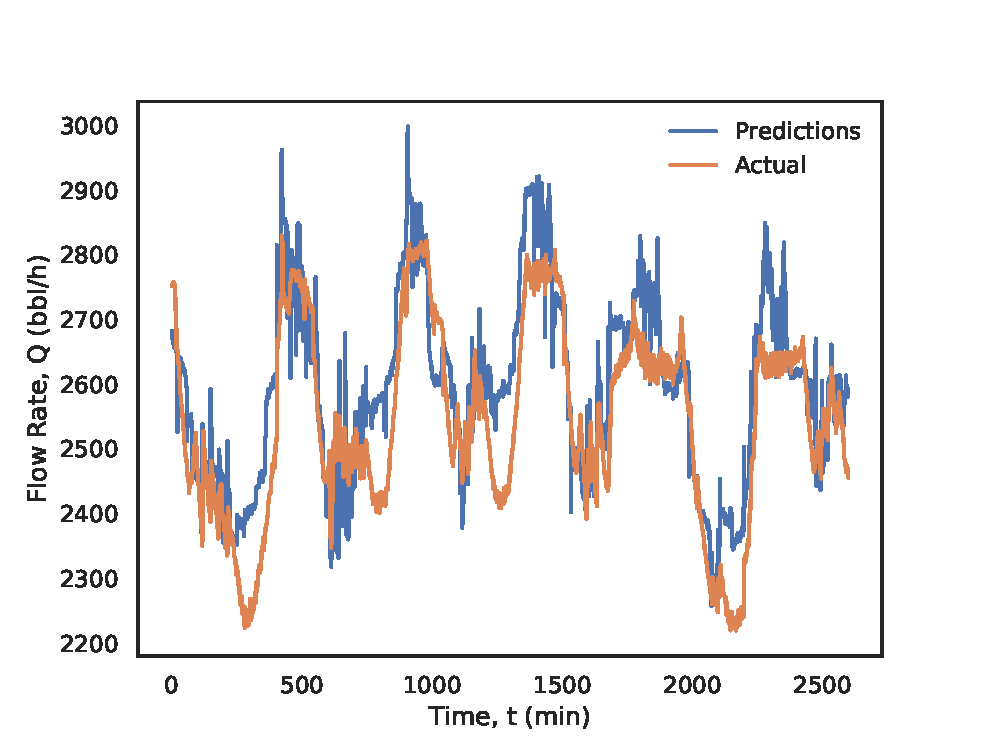
\includegraphics[width=\textwidth]{images/suncor/08cluster1_test.eps}
         \caption{Test data using model 1.}
         \label{fig:02cluster1_test}
     \end{subfigure}
     \begin{subfigure}[b]{0.48\textwidth}
         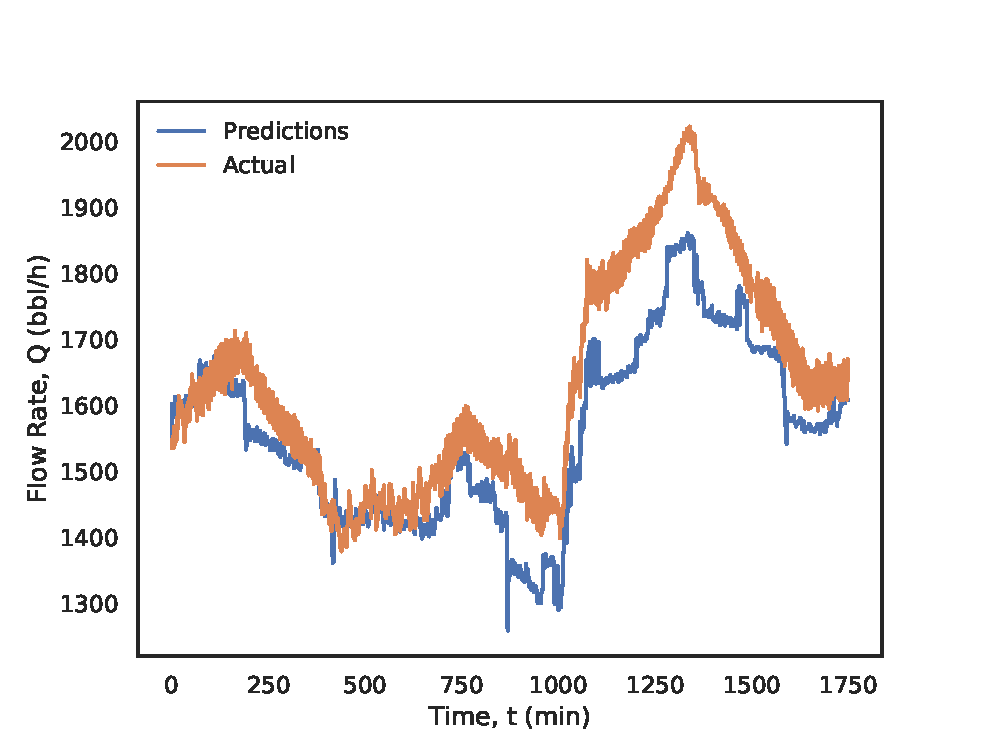
\includegraphics[width=\textwidth]{images/suncor/08cluster2_valid.eps}
         \caption{Validation data using model 2.}
         \label{fig:02cluster2_valid}
     \end{subfigure}
     \begin{subfigure}[b]{0.48\textwidth}
         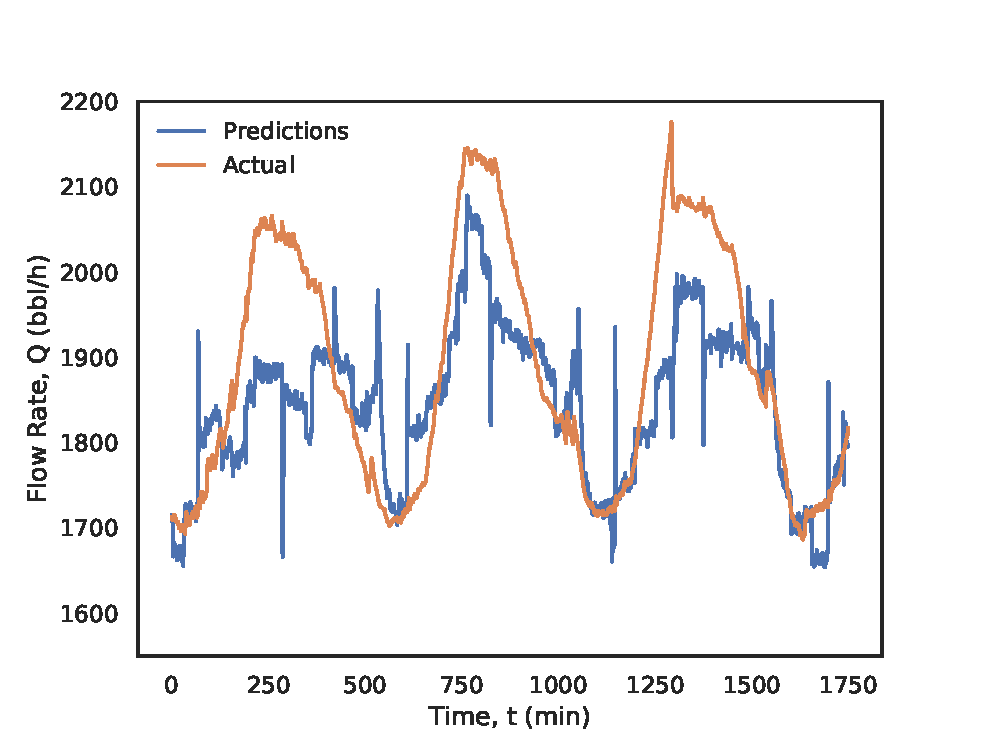
\includegraphics[width=\textwidth]{images/suncor/08cluster2_test.eps}
         \caption{Test data using model 2.}
         \label{fig:02cluster2_test}
     \end{subfigure}
        \caption{Predicted vs. actual flow rate for the linear parameter-varying models.}
        \label{fig:02LPVPlots}
\end{figure}

\subsection{Implementation of USIS}
After the model accuracy was deemed acceptable by the industrial sponsors, the next phase of the project aimed to automate machine learning updates, creating a true self-learning system.  The USIS algorithm was applied to automate each update step, while avoiding outliers and catastrophic interference. 

The hyper parameters for USIS are summarized in Table \ref{tab:02USISHP}. The model was set to update every 24 hours to avoid any significant changes in model weights. Each update step has a maximum of 1440 ($24 \times 60)$ data points per bin. There were ten bins for each model; each had a width of 200 bbl/h.  The bins ranged from 1200 - 3200 bbl/h.  The Euclidean distance was used to calculate the distance metric, $d$.  Moreover, the neglect parameter was selected to be 1.13, identical to $\epsilon$.  Finally, each replay buffer had the capacity to keep three months data in memory to avoid catastrophic interference.  Three months was recommended by the industrial sponsors to ensure relevant information was used for model updates.

\begin{table}[h]
    \centering
    {\setstretch{1.2}
    \begin{tabular}{c|c}
    Hyper parameter & Value \\ \hline
    \# of models, $n$ & 2 \\
    Model update frequency & 24 hrs \\
    Bin size, (bbl/h) & 200 \\
    Distance metric, $d$ & Euclidean \\
    Neglect parameter, $\eta$ & 1.13 \\
    Replay buffer & 129,600 (3 months) \\
    \end{tabular}}
    \caption{USIS hyper parameters for the pipeline project.}
    \label{tab:02USISHP}
\end{table}

The overall USIS algorithm implemented onto the industrial pipeline is shown in Figure \ref{fig:02USISPipe}.  Raw process data is first inputted into the data pre-processing step where data is smoothed (temperature, DRA), transformed (density data), and normalized.  The processed data is then sent into the model selection phase, where one of the two linear models will be selected to perform the prediction.  Then, the data is archived in the USIS architecture.  After every 24 hours, the models are updated using historical data.

\begin{figure}[h]
    \centering
    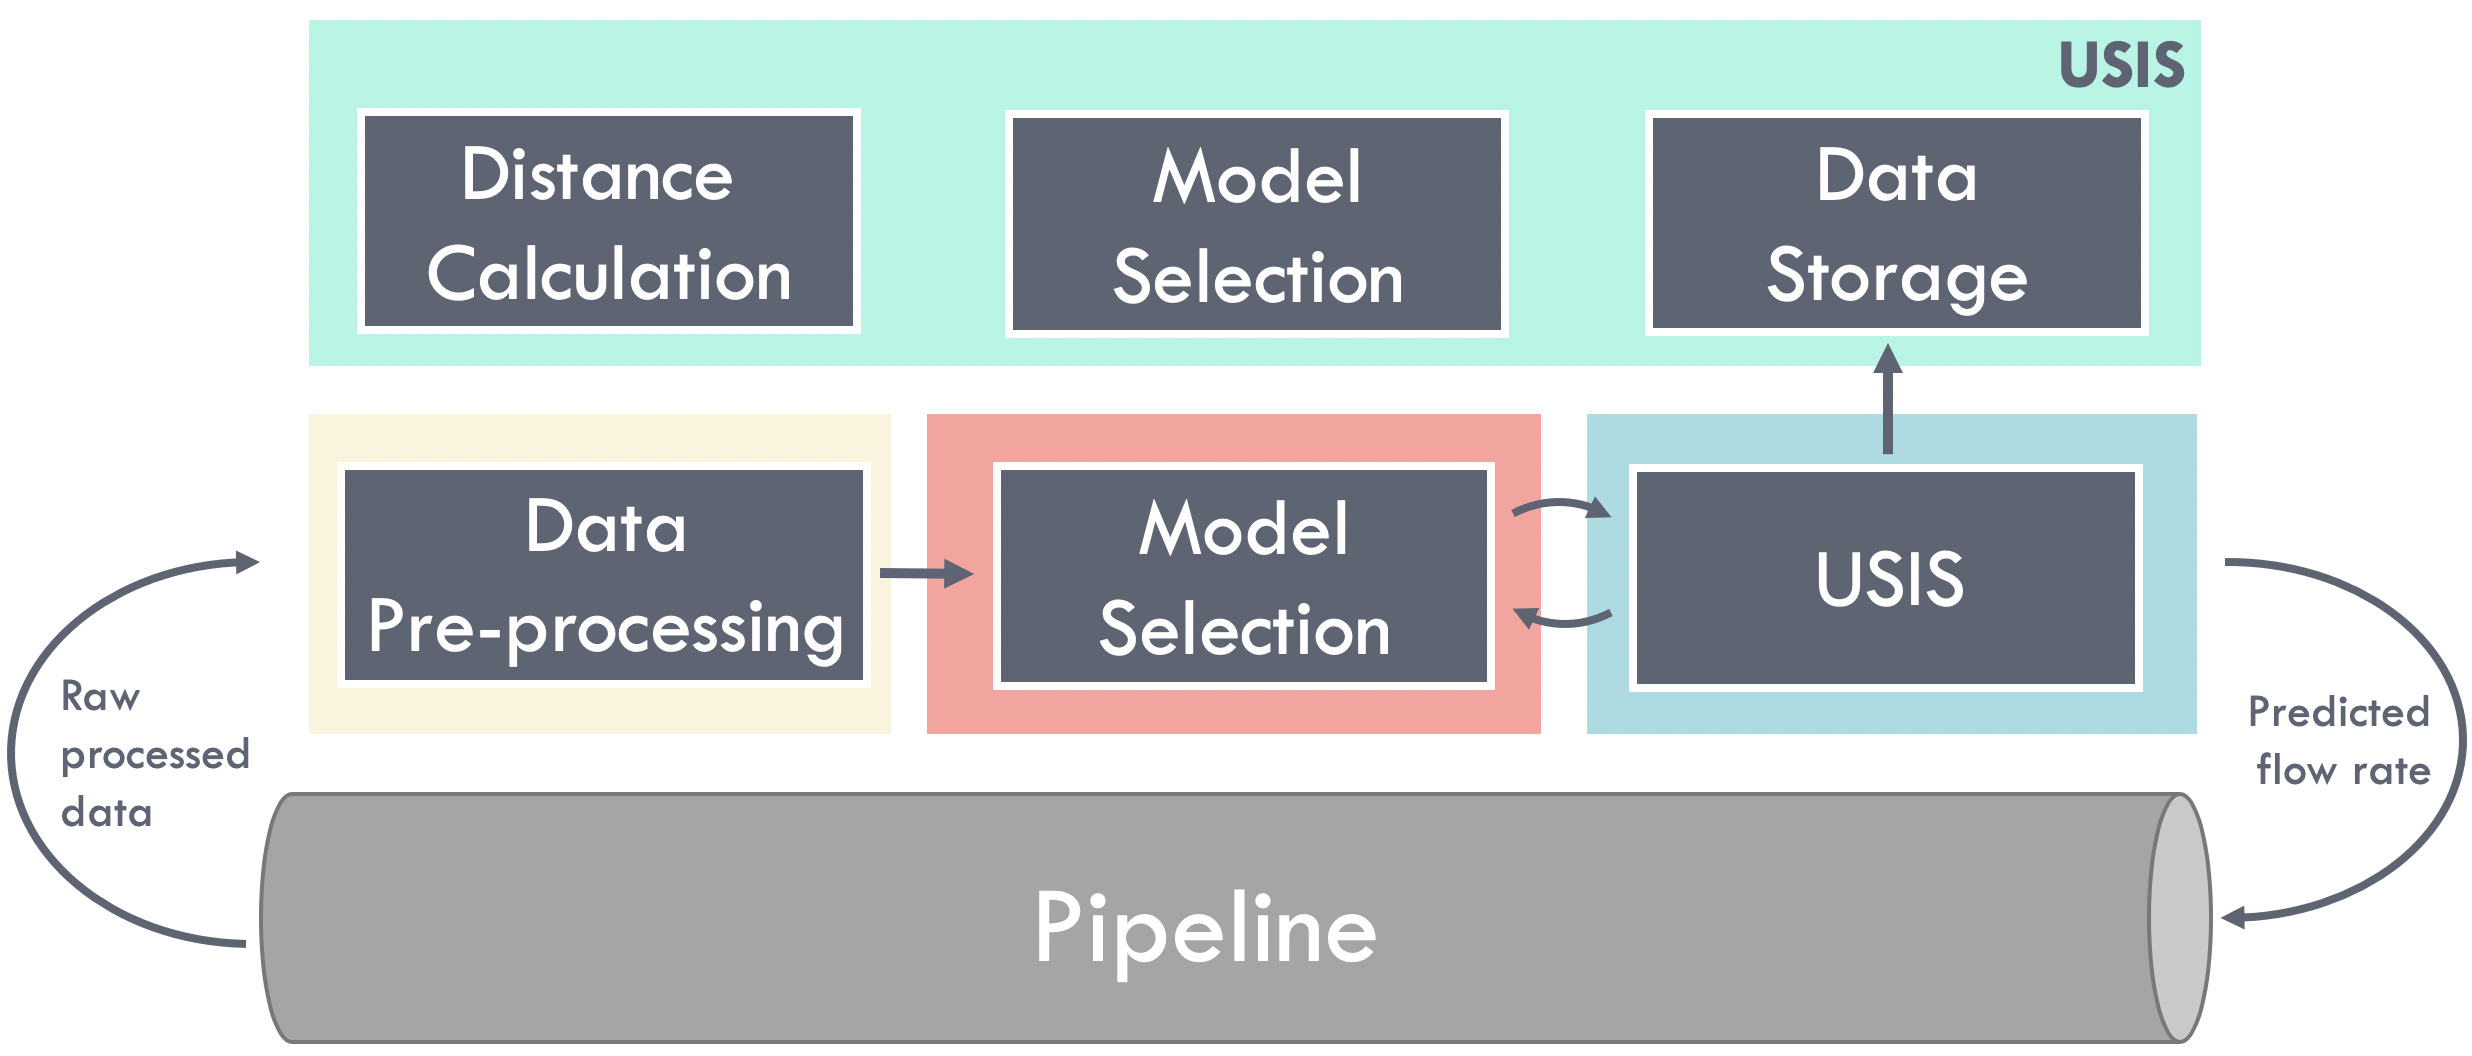
\includegraphics[width=\textwidth]{images/ch2/02USISPipe.jpeg}
    \caption{An overall look at the USIS algorithm on the industrial pipeline}
    \label{fig:02USISPipe}
\end{figure}

\subsection{Concluding Remarks on the Pipeline Project}
Pipelines are critical assets used to transport fluids across large distances.  Common transported fluids include petroleum products, water, sewage, and natural gas. Due to the mission critical nature of pipelines on society's success, ensuring its reliability and efficiency has global-scale impact. 

The first phase of the pipeline project aimed to identify accurate, interpretable, and adaptive models to predict for the output flow rate of the pipeline.  To enhance model performance, the data was initially pre-processed vigorously through smoothing, feature selection, feature engineering, and other methods.  During model identification, the following models were tried: linear models, exponential models, neural networks with varying sizes, LPV models.  Ultimately, LPV models were selected due to their interpretability and predictive capabilities. Adaptability is another key topic of this project. The USIS algorithm was equipped onto the LPV models to allow for outlier-free model updates without suffering from catastrophic interference.


\chapter{Machine Learning for Process Monitoring}
%%%%%%%%%%%%%%%%%%%%%%%%%%%%%%%%%%%%%%%%%%%%%%%%%%%%%%%%%%%%%%%%%%%%%%%%%%%%%%%%%%%%%
% Machine Learning in Monitoring
%
% 1. Anomaly detection
%  - Adaptive using classifier updates
% 2. Alarm management
%  - Adaptive using RL
% 
%%%%%%%%%%%%%%%%%%%%%%%%%%%%%%%%%%%%%%%%%%%%%%%%%%%%%%%%%%%%%%%%%%%%%%%%%%%%%%%%%%%

ML prediction applications are effective complements to existing infrastructure in the process industry through soft sensors, state estimation, and forecasting. However, they are limited in applications regarding safety and risk management.  In the process industry, safety is upheld as the greatest \textit{value}; investing in a successful safety system is just good business.  

\begin{quote}
    "Safety is a \textbf{value}, not a priority.  Priorities change, but company values never do." \\
    --- Rex Tillerson, ex-CEO of ExxonMobil
\end{quote}

Decades ago, process safety investments are frowned upon by management due to its high costs and \textit{invisible} returns. In fact, construction workers used to cheer when project supervisors announced that \textit{only} 20 deaths will incur for this project---an event completely unacceptable in today's standards. Indeed, a perfect safety and risk management system results in \textit{no change} in day-to-day activities because all the incidents are proactively mitigated. As such, it is incredibly easy to become complacent towards risk management. However, if safety takes a back seat, the occurrence of the next incident is not a matter of if, its a matter of \textit{when}. Therefore, safety must be proactively (not reactively) managed to safeguard people, the environment, company assets, and production capabilities in terms of physical equipment and the social license to operate. Here, ML can be leveraged to proactively monitor process systems and create an additional layer of safety. In this chapter, ML algorithms will be applied to detect and predict equipment failures, process abnormalities, process variability and also perform alarm management. Through these applications, ML will be used to create multi-variate alarm systems that explore multi-variable interaction effects and gives fewer false alarms. Additionally, a new alarm management system that specifically tackles alarm flood scenarios will be introduced.  The objectives of this system are twofold: 1) Reduce sheer number of alarms during a flooding scenario; 2) identify the most important alarms so operators can prioritize safety critical alarms.

This chapter is organized as follows: Section 1 introduces data pre-processing methods for anomaly detection/prediction applications where the data is heavily imbalanced.  Section 2 introduces the anomaly detection and prediction algorithms and section 3 concludes this chapter with an introduction to a novel approach for alarm management.

The main contributions of this chapter are the data pre-processing methods used to prepare data sets for anomaly detection/prediction.  Additionally, it was shown that using synthetic data was able to enhance accuracy.  Lastly, a novel alarm management approach based on reinforcement learning was introduced to filter nuisance alarms and sort alarms based on their priority.  




Heavily unbalanced data:
- SMOTE, ADASYN, Breaking time down into smaller segments and increasing sampling rate

\section{Data Pre-processing for Monitoring}
Data containing anomalous and/or incident events are extremely rare---thankfully---in the process industry. \begin{quote}
    Anomaly or anomalous activity: An abnormal or unexpected event given other variables (often multivariate).  For example, a person walking in a t-shirt when it is -$\ang{30}$ C outside.
\end{quote}

In fact, it is not uncommon to have just one incident in a data set containing hundreds of thousands of records.  Under such circumstances, building ML models to identify incidents is extremely difficult.  Remember, ML models are nothing more than statistical models with training formulated in an incremental updating fashion. In the scenario where the training data set contains 999,999 non-anomalous activities with 1 anomalous activity, the model will simply learn to return non-anomalous for all inputs; such a model would still achieve 99.9999\% accuracy on the training data!  When a human is provided with this data set, the human would instead focus most of its attention on the one anomalous activity, studying how it is different from all the other points.  A \textit{tabula rasa} machine is simply not equipped with such cognitive abilities, and will treat every data point equally; however, humans can artificially provide cognition to the machine.

\subsection{Data Prep for Anomaly Detection}
Anomaly \textit{detection} tasks are quite simple compared to anomaly \textit{prediction} tasks that will be discussed later on in this section. In anomaly detection, the model simply has to classify if there is an anomaly at current time. For example, given some states of a reactor, is the output temperature anomalous? That is, is the measured output temperature expected given the states?  Of course, such questions are difficult for humans to answer, especially in multi-variate environments; however, such questions can easily be answered by machines. Unfortunately, the events that are of interest to us (anomalies) are, often times, significantly more rare compared to normal process data. Hence, the leading reason for poor model performance in imbalanced data sets (i.e., distribution of different classes are vastly different) is the \textit{imbalanced} nature.  There exists two traditional ways to tackle the data imbalance issue: \textbf{undersampling} and \textbf{oversampling}.  Objectively, both methods aim to re-balance the data set so that the positive and negative data are in harmony.

A visual description of undersampling and oversampling is shown in Figure \ref{fig:03under_over_sampling}. In undersampling, 

\begin{figure}[H]
    \centering
    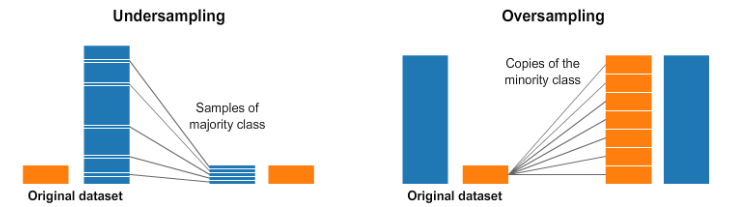
\includegraphics[width=0.8\textwidth]{images/ch3/over_and_undersampling.jpeg}
    \caption{A visual representation of undersampling (left) and oversampling (right). Original image from Kaggle.}
    \label{fig:03under_over_sampling}
\end{figure}

\subsection{Data Prep. for Anomaly Prediction}

\subsection{Synthetic Data Generation}


\section{Anomaly detection and prediction}


The model structure for logistic regression is given as:
\begin{equation}
    \hat{y} = \frac{1}{1 + e^{-(W_1^Tx + W_2^Tu + b)}}
    \label{eq:02LogS}
\end{equation}
where $e$ denotes the exponential operator.

- Measure process variability?

\subsection{Deep Learning Classification and Prediction}

\subsection{Explanability}
- Explanability through weights, through importance sampling

\section{Alarm Management}

\subsection{Alarm Prioritization}

\subsection{Alarm Reduction}


% \chapter{Machine Learning for Control Applications}
% %%%%%%%%%%%%%%%%%%%%%%%%%%%%%%%%%%%%%%%%%%%%%%%%%%%%%%%%%%%%%%%%%%%%%%%%%%%%%%%%%%%%%
% Machine Learning in Control
%
% 1. Reinforcement learning Q-learning algorithm
%  - Extension to of tabular methods to continuous processes using interpolation
%  - Can be extended further using neighbourhood information
% 2. Continuous control using deep reinforcement learning
% 3. Comparison of results with MPC on simple systems
% 4. Fault tolerant RL vs. traditional methods
% 5. Control of a wastewater treatment process
% 6. Optimization
%  - Adaptive using model updates
% 
%%%%%%%%%%%%%%%%%%%%%%%%%%%%%%%%%%%%%%%%%%%%%%%%%%%%%%%%%%%%%%%%%%%%%%%%%%%%%%%%%%%
Advanced process control and optimal control have traditionally used mathematically programming based trajectory optimization methods \cite{empc2, zone_mpc, mpc, empc1,}.  The effectiveness of these methods in addressing multi-stage optimal control problems have been widely demonstrated; however, industrial scale application of such methods in stochastic multiple-input multiple-output (MIMO) systems are still limited due to design and computation complications \cite{MS}. For example, accurate model identification of complex MIMO non-linear systems are nearly impossible. Even if a model were to exist, the computational cost for the non-linear program could be infeasible for online applications. Furthermore, the optimized trajectory to systems containing uncertainty use stochastic programming with only a finite number of uncertainty scenarios and uncertainty information is assumed to be known. In practice, such information are typically unknown, non-stationary and are uncertain themselves \cite{jayCCE}. Moreover, the prediction and control horizon of the trajectory optimization for large MIMO systems are generally truncated to ensure feasible computation time. Though, the identified optimal trajectory for short horizons are typically local optimal solutions \cite{mpc}. Lastly, MP methods require accurate dynamical system models (although no models are perfect in real life); intuitively bottlenecking the optimality of the solution, a scenario similar to supervised learning.

Comparatively, RL online computational times are significantly shorter even for long control horizons or large-scale MIMO systems because the optimal solutions are pre-computed and stored offline, a concept similar to explicit model predictive control (MPC) where parametric programming is used \cite{explicit_MPC}. Furthermore, RL finds the optimal policy through meaningful interactions with the environment.  After each interaction, values are assigned/updated for the visited state. The value functions are stored for future decision making.  Through this identification process, the value functions implicitly contain the uncertainty information of all $x \in \mathcal{X}$. From these unique features of RL in control applications, it is a natural curiosity to explore its potential in the process control industry.

The contributions made in this chapter are as follows:
\begin{enumerate}
    \item Introduction of a simple, cost-effective, and explainable RL algorithm for process control.  The method is also continuous and non-linear.
    \item Compared RL and deep RL to traditional optimal control methods such as MPC.
    \item Applied RL to an industrial grade waste water treatment plant (WWTP) for optimal control.  Results were compared to MPC, economic MPC, and distributed MPC frameworks.
    \item Applied RL for fault prediction and fault tolerant control applications.
\end{enumerate}


\section{An direct adaptive optimal control method}
On a high level, optimal control methods extremize the functional equation of a system through MP methods. In literature, it was found that optimal control methods are less tractable both computationally and analytically compared to set-point tracking or regulations methods (due to non-convex optimization among factors). Consequently, adaptive optimal control methods have received less academic attention, with most existing studies focused on indirect methods like model re-parameterization \cite{rl_control}.  In \cite{rl_control}, RL was shown to be an effective \textit{direct} optimal control method as it adapts its control policy directly. Direct adaptive optimal control methods are especially useful for systems where accurate models are not identifiable and/or available.  In such scenarios, in-direct methods struggle because the accuracy of the model is paramount for successful control.  On the other hand, direct methods can update the control policy directly through interactions with the system, eventually arriving at the optimal policy. In \cite{power_control}, the authors showcased RL's directly adaptive nature by applying an agent onto the control system of a data-center cooling application. In such systems, accurate models are nearly impossible to identify due to complex non-linear relationships between thousands of variables. However, the agent here was able to adapt to the optimal policy directly after sufficient online interactions which ultimately resulted in 22\% reduced power consumption compared to model-based approaches.  Likewise, \cite{power_control2} applied RL onto power systems with ever-changing load fluctuations.  Again, such a system is nearly impossible to model through traditional means; however, the agent was still able to adapt its policy after sufficient online interactions. Wireless networks is a third system with nearly unidentifiable dynamics. The authors in \cite{power_control3} demonstrated deep RL's direct adaptive nature through its application onto wireless networks, ultimately resulting in superior control compared to all previous methods.

\section{Controlling a VFD using $Q$-learning}
A detailed quantitative example is provided in this section to serve as a gentle introduction of RL's applicability in process control systems \footnote{For further intuition, the supplementary code for all results generated in this section are located at: https://github.com/RuiNian7319/Research/tree/master/2.RL\_Codes/Mechatronix}. Here, the \textit{off-policy} tabular $Q$-learning algorithm with upper confidence bound (learning acceleration heuristics) was used for output pressure tracking of an industrial variable frequency drive (VFD) pump. 

\subsection{System Description}
The industrial VFD system is built by Turbine Technologies and is called the FLUIDMechatronix.  On the system, there exists thousands of different tags measuring countless states. For this control example, the output pressure, $P_{out}$, and pump RPM will be used. From the FLUIDMechatronix manual, the safe operating ranges of the pressure and pump RPM are:
$$0 \; kPa \leq P  \leq 45 \; kPa$$
$$0 \; Hz \leq RPM  \leq 60 \; Hz$$
In terms of system representation, a FOMDP will be used because all system measurements are available and the system dynamics are fast. Initially, the system starts in:
\begin{equation}
    P_0 = 41 \; kPa
    \label{eq:initial_p}
\end{equation}
\begin{equation}
    u_0 = 60 \; RPM
    \label{eq:initial_u}
\end{equation}

\begin{figure}[H]
    \centering
    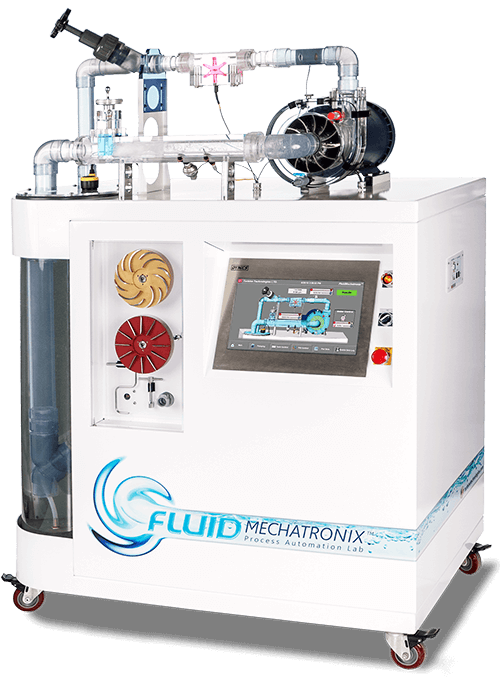
\includegraphics[width=0.38\textwidth]{images/ch4/Mechatronix.jpeg}
    \caption{The FLUIDMechatronix experiment from Turbine Technologies \cite{turbine}.}
    \label{fig:mechatronix}
\end{figure}

Implementing RL for the control of an industrial process typically involves four steps: i) Model identification; ii) agent design; iii) initial training; iv) online calibration.  The details of each step are shown in \ref{fig:rl_implementation}.

\begin{figure}[H]
    \centering
    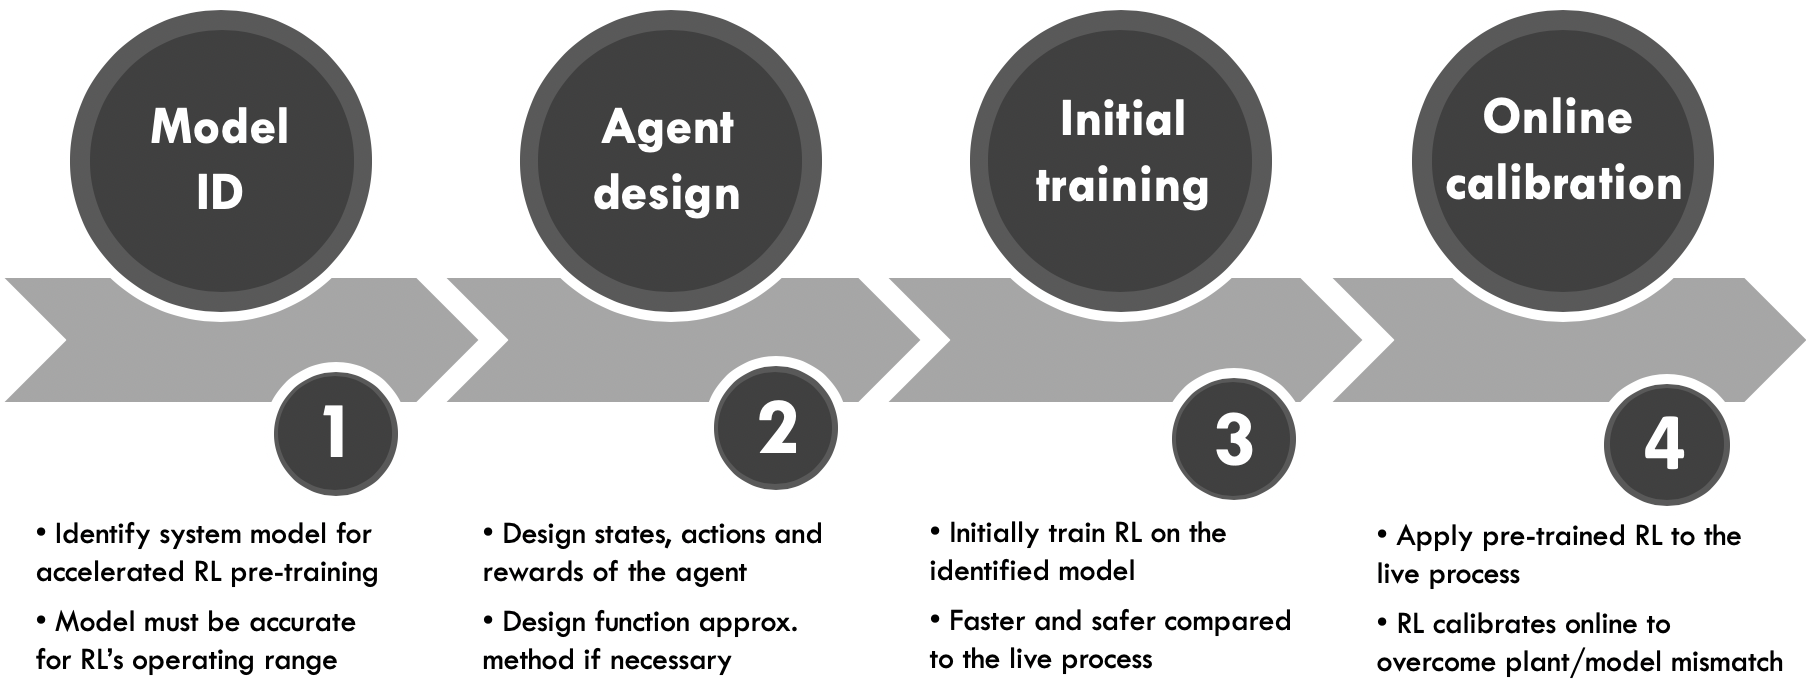
\includegraphics[width=0.95\textwidth]{images/ch4/RL_implementation.jpeg}
    \caption{General procedure for implementing industrial reinforcement learning.}
    \label{fig:rl_implementation}
\end{figure}

\subsection{Step 1: Model ID}
One major drawback of RL is its unreasonable data efficiency.  In fact, it \textit{may} take thousands of interactions before anything meaningful is first learned.  As such, implementing RL to learn online is time-infeasible because decades may pass before the optimal policy is identified.  To overcome this flaw, a \textit{representative} simulation model can first be constructed to pre-train the agent offline.  After adequate performance is observed in simulation, the agent can be implemented online.  Initially, the agent will calibrate its policy to the live process to overcome any model-plant mismatches. The time required for calibration is heavily dependent on the accuracy of the simulation model.  For perfectly representative models, such as video games, a calibration time is not required. Afterwards, optimal control can commence.

For model identification, pseudo-random input signals were used to provide excitation to the VFD for input-out data generation. The data collection process was terminated after 18,000 input-output signals were obtained. Then, a quadratic model was identified using least squares. The identified model is given as:
\begin{equation}
    P_{out} = 0.012 \cdot RPM^2 + 0.024 \cdot RPM - 2.073
\end{equation}
The mean squared error (MSE) of the identified model was 0.056 and the fitted model compared to the experimental data is shown in Figure \ref{fig:04model_fit}.
\begin{figure}[H]
    \centering
    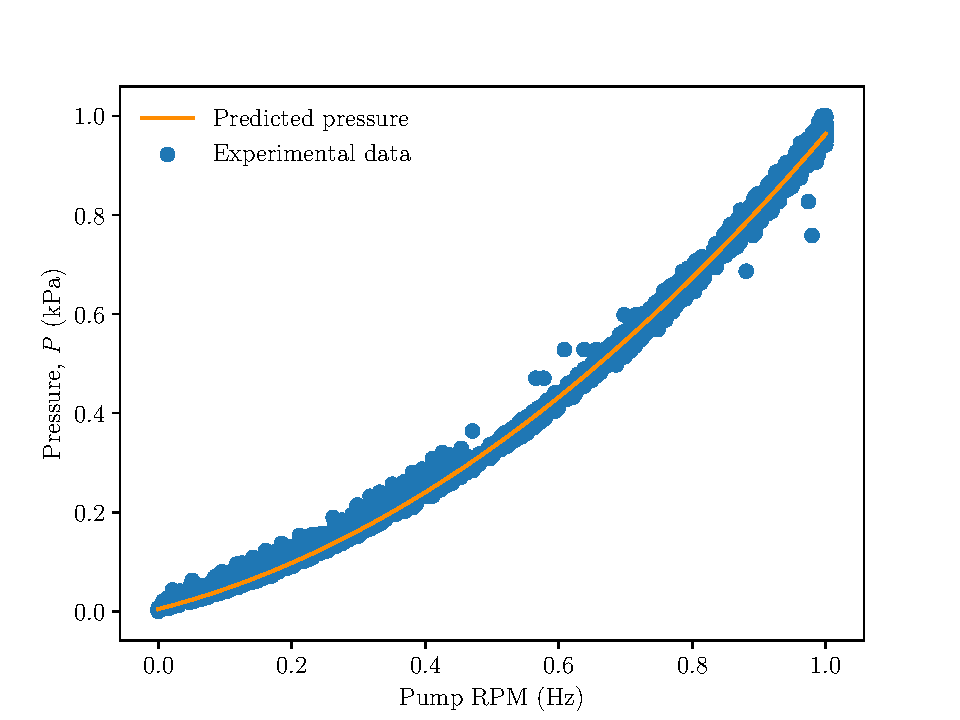
\includegraphics[width=0.7\textwidth]{images/ch4/model_fit.pdf}
    \caption{Performance of the identified system model on a test data set.}
    \label{fig:04model_fit}
\end{figure}

\subsection{Step 2: Agent design}
The overall RL paradigm for this example is shown in Figure \ref{fig:04rl_system1}. Intuitively, the agent tracks a set-point for the output pressure by manipulating the pump RPM.  To allow for the tracking of a variable set-point, the state of the agent is the current tracking error:
\begin{equation}
    \varepsilon = P_t - P_{t, sp}
\end{equation}
and the action is the \textit{change} in pump RPM $\Delta u$. Here, $P_t$ is the pressure at time $t$ and $sp$ denotes the set-point. This \textit{velocity} based implementation is a requirement for tracking multiple set-points. If the action was the pump RPM instead (and not $\Delta u$), then the agent would fail to track multiple set-points since it simply maps different tracking errors to one pump RPM that corresponds to \textit{one} set-point. For example, suppose the current set-point is $10 \; kPa$ and $P_t = 0$ resulting in a -10 tracking error. Here, suppose the optimal RPM is $u = 20$. After implementing $u = 20$, the system reaches steady state and achieves a tracking error of 0. After some time, the machine operator may then decide to change the set-point to $20 \; kPa$. Now again, the tracking error is -10; however, the RPM from the agent would still be $u = 20$ because the state-action is a 1 to 1 mapping; thus, unable to track any changes in set-points. 

The reward function of the agent is given by:
\begin{equation}
    r(x, u) = max(-\varepsilon^2 - \Delta u, -200)
\end{equation}
where $\Delta u$ is the change in input to discourage the agent from making unnecessary actions. Additionally, the reward is clipped to -200 for convergence properties and to avoid numerical issues as explained in the reward clipping section. The upper reward limit is not clipped because the function is naturally capped at 0. Here, the agent evaluates every five seconds to guarantee that steady state has been reached before consecutive actions are made. Five seconds was chosen because it was identified to be the longest transition time required. Moreover, the decision making would not be Markovian (i.e., observed states are not independent of the past because the states do not provide the transition information to the agent) if the agent evaluates during the transition period. In such scenarios, the agent will fail to learn anything meaningful. 

\begin{figure}[H]
    \centering
    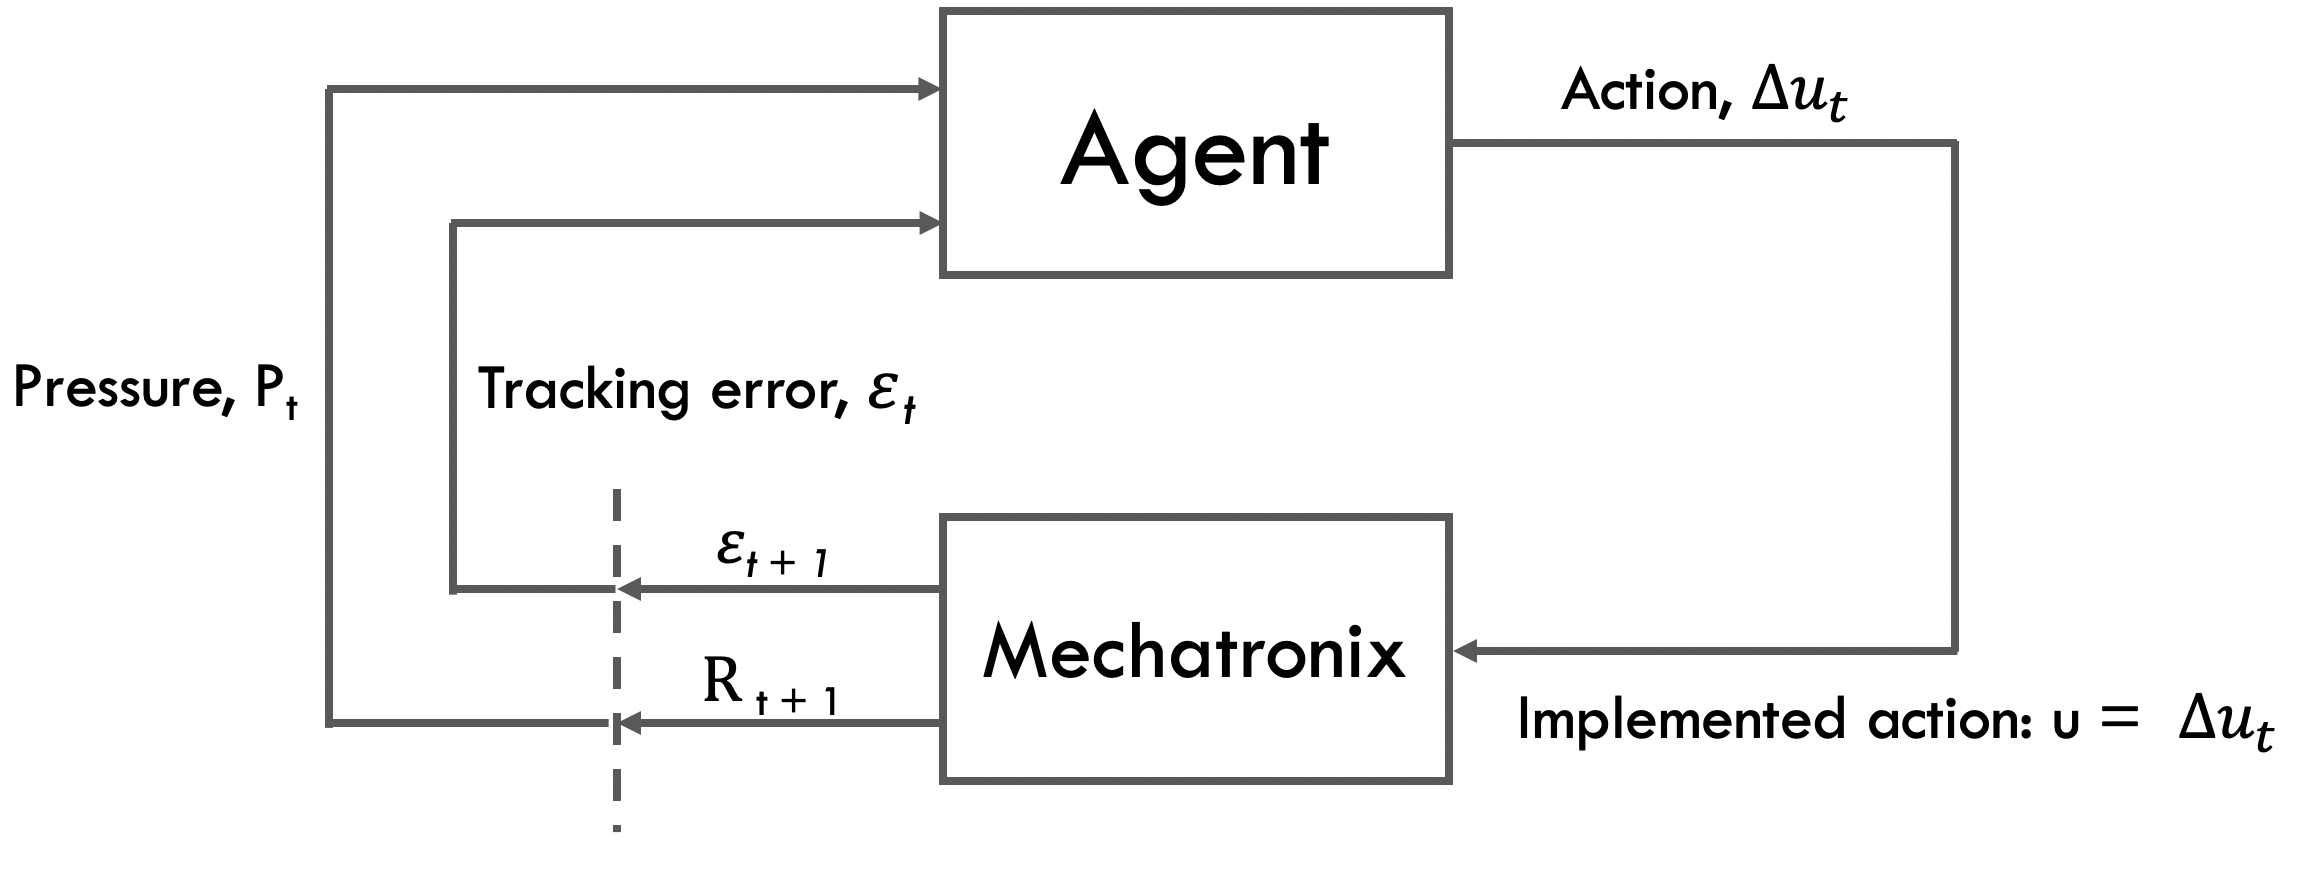
\includegraphics[width=0.7\textwidth]{images/ch4/rl_system1}
    \caption{The RL set-up for the FLUIDMechatronix experiment.}
    \label{fig:04rl_system1}
\end{figure}

All hyper parameters of the agent are shown in Table \ref{tab:rl_system1_params}. The states and actions of the agent are discretized as:
\begin{equation}
    x = [-20, -19, ..., 20]_{1 \times 41}
\end{equation}
\begin{equation}
    u = [-10, -9, ..., 10]_{1 \times 21}
\end{equation}
totalling 861 different action-values to identify. Furthermore, the $Q$-matrix storing all the action-value functions is shown in Figure \ref{fig:q_matrix_system1}.  The agent is initiated with all action-values as 0, a condition known as \textit{tabula rasa}.
\begin{figure}[H]
    \centering
    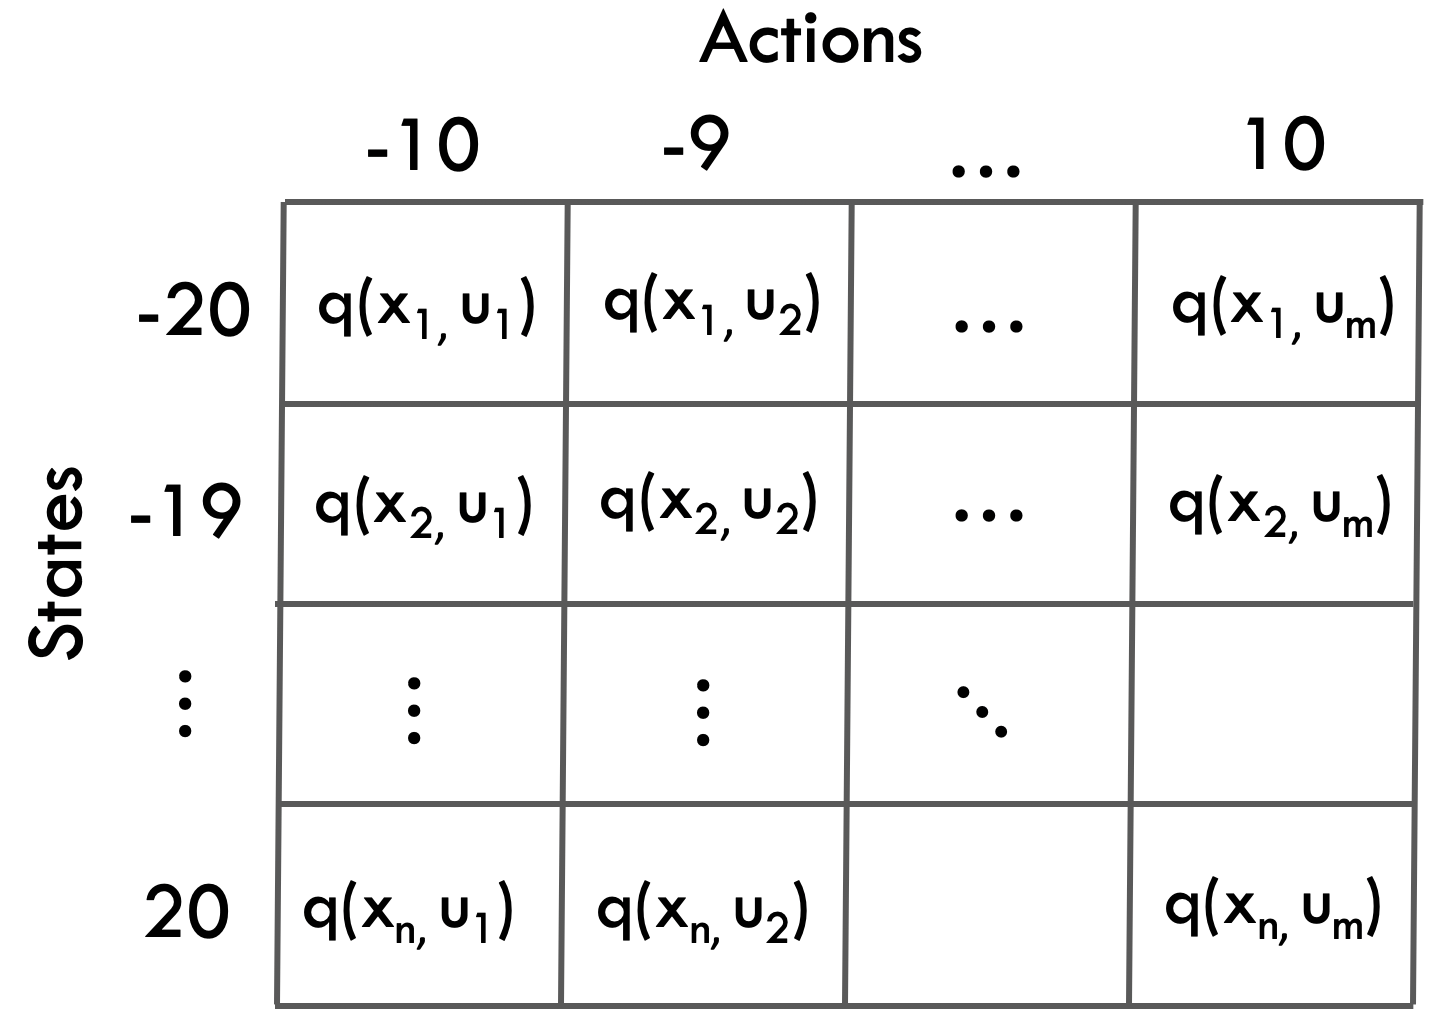
\includegraphics[width=0.5\textwidth]{images/ch4/q_matrix_system1.jpeg}
    \caption{$Q$-matrix of the Mechatronix system.}
    \label{fig:q_matrix_system1}
\end{figure}
The states and actions on the axis of the $Q$-matrix correspond to $\varepsilon$ and $\Delta u$, respectively.  The discount factor, $\gamma$, was 0.9. Altogether, 2,000,000 time steps were used to train the agent (corresponding to 115.7 days of continuous operating experience). After every 400$^{th}$ time step, the agent's state and action was reset back to Equations \ref{eq:initial_p} and \ref{eq:initial_u} to prevent extreme controller saturation. 

The agent uses a equiprobable random exploratory policy ($\epsilon$ = 1) to conduct initial exploration. Throughout training, $\epsilon$ is slowly and linearly decayed until $\epsilon = 0.1$ by the 500,000$^{th}$ update. Likewise, the learning rate is initiated at 0.7 and also linearly decay until 0.001.

\begin{table}[H]
\caption{Summary of the agent's hyper parameters in the Mechatronix experiment.}
\label{tab:rl_system1_params}
\centering
\begin{tabular}{c|c}
\textbf{Hyper Parameter}     & Value  \\
\hline
States, $x$	             	& $\varepsilon = [-20, -19, ..., 20]_{1 \times 41} $		 \\
Actions, $u$               & $\Delta u = [-10, -9, ..., 10]_{1 \times 21}$		\\
Reward, $r$	               & max($-(\varepsilon^2 + \Delta u)$, -200)		\\
Learning rate, $\alpha$		& [0.001, 0.7]		 \\
Discount factor, $\gamma$      	& 0.9  \\
Exploratory factor, $\epsilon$             & [0.1, 1]  \\
Evaluation time                 & 5 seconds \\
System representation           & FOMDP \\
\end{tabular}
\end{table}

\subsection{Step 3: Initial training}
The agent behave as follows: the agent observes some initial tracking error $\varepsilon_t$ and performs a random action $\Delta u_t$ with accordance to its behaviour policy (initially equiprobable random).  Next, the pump RPM corresponding to $u_t = u_{t-1} + \Delta u_t$ is sent to Mechatronix.  After five seconds, the agent receives reward $R_{t+1}$ and then observes new tracking error, $\varepsilon_{t+1}$. Using the tuple $(x_t, u_t, r_{t+1}, x_{t+1})$, the agent updates its current knowledge via Equation \ref{eq:q_learning}. This step is repeated many times until the optimal policy, $\pi^*$, is identified. A numerical walk-through of the calculations is shown below:

\begin{quote}
    Suppose another simpler agent was constructed for this system. For this agent, the system was discretized into five states and three actions:
    $$x = [-21, -10, 0, 10, 21]_{1 \times 5}$$
    $$u = [-1, 0, 1]_{1 \times 3} $$
    Consequently, the $Q$-matrix was initialized as:
    
    $$ Q(x, u) = \left(\begin{matrix}   0 & 0 & 0 \\
                                        0 & 0 & 0 \\
                                        0 & 0 & 0 \\
                                        0 & 0 & 0 \\
                                        0 & 0 & 0 \end{matrix}\right) $$
    
    where the rows and columns correspond to the different states and actions, respectively. The system's set-point was initially at 30 kPa. The agent was initiated at steady state with 15 kPa and 37 RPM, resulting in $\varepsilon=-15$. At $t = 0$, the agent receives the error and rounds it to the nearest discretized value, $x = -10$.  Given this state, the agent uses the $Q$-table and picks the action that corresponds to the highest $Q$ value (note if a equiprobable random policy was initially followed, a random action would be selected instead):

        $$Q(-10, u) = [0, 0, 0]$$

    where the three values correspond to the predicted action-values for selecting actions $\Delta u = -1, 0, -1$, respectively. Since the agent is inexperienced and have not been provided with prior information about the system, it thinks that all three actions are indifferent; therefore, the agent will pick an arbitrarily action to learn more about the system. Moreover, during scenarios where $Q^{max} = Q_1 = Q_2 = ... = Q_n$, ties \textit{must} be broken arbitrarily to avoid biasing one action over all others.
    
    Assuming that $u = -1$ was picked, the system will transition to 13.8 kPa. After five seconds, the new observed tracking error would be -16.2. Clearly, this was a sub-optimal action; if the pressure was already lower than the set-point, it would be intuitive to increase pump RPM instead. However, a \textit{tabula rasa} agent is not aware of such a phenomenon, humans only know this through prior experience. Here, the agent would also receive reward:
    $$max(-16.2^2 - 1, -200) = -200$$ 
    and be in new state $x_1 = -21$.  From this interaction, the agent would then update the $Q$-matrix using Equation \ref{eq:q_learning}:
    $$Q(-10, -1) \leftarrow Q(-10, -1) + 0.7 [-200 + \gamma Q(-21, 0) - Q(-10, -1)]$$
    $$Q(-10, -1) \leftarrow 0 + 0.7 [-200 + 0.9 \cdot 0 - 0]$$
    $$Q(-10, -1) \leftarrow -140 $$
    and the updated $Q$-matrix would be given as:
    
    $$ Q(x, u) = \left(\begin{matrix}   0  &  0  & 0 \\
                                        -140 & 0 & 0 \\
                                        0 & 0 & 0 \\
                                        0 & 0 & 0 \\
                                        0 & 0 & 0 \end{matrix}\right) $$
                                        
    In this case, all three $u$'s for $Q(x_{t+1}, u_{t+1})$ are also reward maximizing; therefore, the ties are here must also be broken randomly to avoid unnecessary bias. Suppose the system was reset, initiating at $x_0 = -10$.  This time, the $Q$-matrix provides:
    
    $$Q(-10, u) = [-140, 0, 0]$$
    
    telling the agent that $\Delta u = -1$ is a sub-optimal compared to $\Delta u = 0 \text{ or } 1$.  For a reward maximizing agent, either $\Delta u = 0 \text{ or } 1$ would be picked instead.  
    
    After many interactions with the system, the $Q$-matrix now becomes:
    
        $$ Q(x, u) = \left(\begin{matrix}   -152  &  -133  & -120 \\
                                        -149 & -121 & -99 \\
                                        -31 & -22 & -33 \\
                                        -102 & -142 & -162 \\
                                        -152 & -162 & -177 \end{matrix}\right) $$
    
    Now, the agent has vastly more knowledge about the system and can begin acting optimally. After resetting the agent back to $x_0 = -10$, the decision making of the agent is now deterministic.  The corresponding action-values given $x_0 = -10$ are:
    
    $$Q(-10, u) = [-149, -121, -99]$$
    
    Here, the agent would pick $\Delta u = 1$ corresponding to $Q(-10, 3) = -99$ (greedy action) and the system would transition to $P_1 = 16 \; kPa$.  Although the error is still closest to -10 (set-point is 30 kPa), the reward obtained is much better compared to actions -1 or 0.  The new update step is given as:
    
    $$Q(-10, 1) \leftarrow Q(-10, 1) + 0.001 [-197 + \gamma Q(-10, 1) - Q(-10, 1)]$$
    $$Q(-10, 1) \leftarrow -99 + 0.001 [-197 + 0.9 \cdot -99 + 99]$$
    $$Q(-10, 1) \leftarrow -99 + 0.001 [-187.1]$$
    $$Q(-10, 1) \leftarrow -99.19 $$
    
    Here, $\alpha$ is much lower compared to previously due to the continuous decay throughout the training process. The currently TD error is -187.1, still quite a high value.  Eventually, all TD errors will approach near-zero and the agent's policy will become optimal.
\end{quote}

The reward obtained across the 2 million training steps is shown in Figure \ref{fig:loss_curve}. Ultimately, the reward was unable to become zero because the lower bound of $\epsilon$ was set to 0.1, forcing exploratory moves even when the agent had the capability of acting optimally. During training, the set-point was drawn from a Gaussian distribution $N(30, 5)$. 
\begin{figure}[H]
    \centering
    \includegraphics[width=0.66\textwidth]{images/ch4/loss_curve.pdf}
    \caption{Loss curve of the agent during training.}
    \label{fig:loss_curve}
\end{figure}

\subsection{Step 4: Online calibration}

The agent was then applied onto the real process to track pressure set-points of 35 and 5.  The output pressure trajectory of the Mechatronix is shown in \ref{fig:system1_highsp} and \ref{fig:system1_lowsp}. Performance-wise, the MSE was $14.2$ and $15.5$ for set-points 35 and 5, respectively. To ensure a fair comparison, both cases started with initial pressures approximately 5.5 kPa above the desired set-point. In this simple set-up, the agent behaves much like a PID where the RL maps tracking errors to changes in input and is linear in nature. Unfortunately, such a set-up only works well locally for non-linear systems. Moreover, the performance decreases significantly as the agent ponders away from the linear region, as shown in Figure \ref{fig:system1_lowsp}. In this experiment, the agent's performance is significantly better when tracking $P=35$ because the training set-points were heavily biased towards $P=35$.  From Figure \ref{fig:04model_fit}, it can be seen quite obviously that the controller gain changes significantly at lower pressures, resulting in the optimal policy for the higher pressure range being completely sub-optimal at lower pressures. Furthermore, the large off-set seen in these trajectories are caused by the discretization error; there exists no action $\Delta u \in \mathcal{U}$ that can obtain exactly $P = 35 \; or \; 5 \; kPa$. To overcome this, one option is to discretize the action space more finely, but this will unavoidably the increase the training time and space complexity required by the agent (perhaps by a massive margin).  A simpler way will be introduced in the latter half of this example.

\begin{figure}[H]
     \centering
     \begin{subfigure}{0.49\textwidth}
         \centering
         \includegraphics[width=\textwidth]{images/ch4/35SP_normal.pdf}
         \caption{Tracking $P_{sp} = 35 \; kPa$}
         \label{fig:system1_highsp}
     \end{subfigure}
     \hfill
     \begin{subfigure}{0.49\textwidth}
         \centering
         \includegraphics[width=\textwidth]{images/ch4/5SP_normal.pdf}
         \caption{Tracking $P_{sp} = 5 \; kPa$}
         \label{fig:system1_lowsp}
     \end{subfigure}
     \caption{Pressure trajectory of the Mechatronix experiment.  Solid line represents the average of 10 runs to ensure reproducability. Shaded area correspond to one standard deviation.}
\end{figure}

\subsection{Extension to Non-linear Systems}
A simple, cost effective way for the agent's capabilities to extend to non-linear systems is to model the system using a linear parameter-varying model as shown in Figure \ref{fig:model_fit_approx}. This way, each sub-piece of the model is linear, allowing even linear control laws to be optimal.  To create a Markovian setting, the agent will receive this information through a \textit{second state} given by:
\[
    x^{(2)}= 
\begin{cases}
    1,              & \text{if } P  \leq 10 \\
    2,              & \text{if } 10 <  P  \leq 20 \\
    3,              & \text{if } 20 <  P  \leq 30 \\
    4,              & \text{if } 30 <  P  \leq 50 \\
    5,              & P > 50 \\
\end{cases}
\]
The new state space for the agent is given by:
\begin{equation}
    x = [(-20, 1), (-20, 2), (-20, 3), ..., (-19, 1), ..., (20, 5)]_{1 \times 205}
\end{equation}
where the first value denotes the error and the second value correspond to the region the agent is currently in. Here, the $Q$-matrix will be initialized as $0_{(41 \cdot 5) \times 3}$ to accommodate for the second state. Intuitively, the agent now observes both the magnitude and the context of the incurred tracking error; intrinsically, allowing the agent to change its policy depending on the region it is currently in.

\begin{figure}[H]
    \centering
    \includegraphics[width=0.62\textwidth]{images/ch4/model_fit_approx.jpeg}
    \caption{Approximating the non-linear Mechatronix system.}
    \label{fig:model_fit_approx}
\end{figure}

The new agent was implemented onto Mechatronix after 2,000,000 time steps of training.  The new agent's output pressure trajectories for tracking $P=35$ and 5 are shown in Figures \ref{fig:system1_highsp2} and \ref{fig:system1_lowsp2}.  Performance-wise, the agent achieved  MSEs of 14.2 and 12.5 for the higher and lower set-point; a massive improvement for the lower set-point.  Nevertheless, the offset still exists.

\begin{figure}[H]
     \centering
     \begin{subfigure}{0.49\textwidth}
         \centering
         \includegraphics[width=\textwidth]{images/ch4/35SP_2state.pdf}
         \caption{Tracking $P_{sp} = 35 \; kPa$}
         \label{fig:system1_highsp2}
     \end{subfigure}
     \hfill
     \begin{subfigure}{0.49\textwidth}
         \centering
         \includegraphics[width=\textwidth]{images/ch4/5SP_2state.pdf}
         \caption{Tracking $P_{sp} = 5 \; kPa$}
         \label{fig:system1_lowsp2}
     \end{subfigure}
     \caption{Pressure trajectory using the non-linear agent. Solid line represents the average of 10 runs to ensure reproducability. Shaded area correspond to one standard deviation.}
\end{figure}



\subsection{Extension to continuous states and actions}
Because the non-linear system was approximated using a LPV model, the control law for the system should be always linear. Because of this, linear interpolation can be used to find the optimal control action using \cite{interpolation}:
\begin{equation}
    u = u_{low} + (x - x_{low})\frac{u_{high} - u_{low}}{x_{high} - x_{low}}
    \label{eq:interpolation}
\end{equation}
where $x$ is the actual tracking error; typically, the exact value of $x$ is not included in the discretized state space $\mathcal{X}$.  Instead, $x$ is typically between $x_{high}$ and $x_{low}$, where $x_{high}$ and $x_{low}$ correspond to the state that is higher and lower than $x$, respectively.  For example, if the discretized state space is given as $x = [0, -5, -10]$ and the current state is -3, $x_{high}$ and $x_{low}$ would be 0 and -5, respectively.  Similarily, $u_{high}$ and $u_{low}$ are the greedy actions for $x_{high}$ and $x_{low}$, respectively. For example, given the action space $u=[-5, 0, 5]$ and $Q-$matrix:

    $$ Q(x, u) = \left(\begin{matrix}   -5  &  2  & 1 \\\
                                        4 & 1 & -2 \\
                                        -2 & 0 & 3 \end{matrix}\right), $$
                                        
$u_{high}$ and $u_{low}$ are 0 and -5 (actions corresponding to the index of the highest $Q$-value), respectively. Moreover, the optimal action for $x = -3$ would be:
$$u = -5 + (-3 + 5) \frac{0 + 5}{0 + 5}$$
$$u = -3$$

With the addition of interpolation action selection, the 2-state RL agent (without re-training the agent) achieved pressure trajectories shown in Figures \ref{fig:system1_highsp3} and \ref{fig:system1_lowsp3} with MSEs of 13.6 and 11.7, respectively. Additionally, it can be seen that the off-set is completely eliminated.

\begin{figure}[H]
     \centering
     \begin{subfigure}{0.49\textwidth}
         \centering
         \includegraphics[width=\textwidth]{images/ch4/35SP_interpolation.pdf}
         \caption{Tracking $P_{sp} = 35 \; kPa$}
         \label{fig:system1_highsp3}
     \end{subfigure}
     \hfill
     \begin{subfigure}{0.49\textwidth}
         \centering
         \includegraphics[width=\textwidth]{images/ch4/5SP_interpolation.pdf}
         \caption{Tracking $P_{sp} = 5 \; kPa$}
         \label{fig:system1_lowsp3}
     \end{subfigure}
     \caption{Pressure trajectory of the non-linear agent using interpolation action selection. Solid line represents the average of 10 runs to ensure reproducability. Shaded area correspond to one standard deviation.}
\end{figure}

The RL methods introduced in this section along with their respective characteristics are summarized in Table \ref{tab:system1_info}. Throughout this tutorial, a simple RL agent was implemented onto an industrial VFD system. It was shown that the vanilla algorithm was unable to handle neither non-linear systems or achieve off-set free control; therefore, simple, implementable techniques that extended the agent's ability to non-linear systems and for off-set free control were introduced. Each state trajectory in this study was replicated on the live systems 10 times to ensure reproducability; the standard deviation for every algorithm was very narrow, representing highly reproducible results (indirectly, less risk).

\begin{table}[H]
\caption{A comparison between RL, MPC in literature, and industrial MPC software.}
\label{tab:system1_info}
\centering
{\scriptsize
\begin{tabular}{c|c|c|c}
 & \textbf{Normal $Q$-learning}	& \textbf{2-state $Q$-learning} & \textbf{2-state interpolated $Q$-learning}\\
 \hline
MSE (High/Low SP)   & 14.2 \& 15.5	& 14.2 \& 12.5   &  13.6 \& 11.7 \\
Offset		& Yes			&  Yes   &  No \\
Non-linear		& No			& Yes   &  Yes \\
\end{tabular}}
\end{table}

In the implementation above, the agent only provided the input for the \textit{immediate} future. A concept very similar to MPC where only the next input is used; however, MPC is considered receding horizon control, where an input trajectory for future steps is also calculated.  Using this trajectory, MPC is viable for short horizon open-loop control.  Comparatively, RL can also conduct receding horizon control. Such RL methods typically employ a model of the system and are called planning methods.  In receding horizon RL, the agent still only outputs the immediate control action; however, it then uses the model to identify the next state and its corresponding optimal control action. The cycle continues until the set control horizon is met.  Additionally, like MPC, the trajectory is heavily inaccurate for long control horizons.

The example shown here is simple, has a pre-set sampling time and does not consider transition dynamics or unobservable states. For systems containing dynamic transition times and to consider systems dynamics, semi-MDPs must be used.  The semi-MDP variant of Q-learning algorithm is \cite{continuous_rl_ref14}:
\begin{equation}
    Q(x, u) \leftarrow Q(x, u) + \alpha \left[\frac{1 - e^{-\beta \tau}}{\beta}r(x, x_{t+1}, u) + e^{-\beta \tau} \max_{u_{t+1}}Q(x_{t+1}, u_{t+1}) - Q(x, u) \right]
\end{equation}
where $r(x_t, x_{t+1}, u)$ is the reward rate and is provided in Equation \ref{eq:reward_rate}. For systems with unmeasurable states, concepts of POMDPs provided in Chapter 1 should be used.

\section{Control of Wastewater Treatment Plant}


















\section{Optimality Evaluation of Reinforcement Learning}
UCB tabular $Q$-learning suffers from discretized states and actions and the curse of dimensionality.  To overcome such issues, deep RL will be explored.  More specifically, this section uses the deep deterministic policy gradient (DDPG) algorithm introduced in Chapter 1. DDPG offers several advantages and disadvantages compared to tabular $Q$-learning.  The advantages are that it can handle continuous states and perform continuous actions. Furthermore, the scalability of the algorithm is greatly enhanced because deep function approximators are used to map states to actions, rather than a $Q$-table. However, these advantages come with some disadvantages.  First and foremost, DDPG is a black box approach and employs four deep neural networks to perform function approximation; therefore, explicitly identifying the control policy for DDPG is nearly impossible. Secondly, the function approximations cause small perturbations in control.  That is, the control outputs can sometimes contain small "jitters" (given an ideal output of 1, DDPG may output values between 0.995 - 1.005).  Intuitively, this is caused by the generality of the algorithm and can be related to humans.  Humans possess perhaps one of the most general intelligence available, yet we are not even capable of drawing a straight line. DDPG follows a similar idea; the algorithm is so general that it sometimes struggle with highly precise actions. For advanced details regarding DDPG, see \cite{ddpg}.  

The objective of this section is to \textbf{explore the optimality} of RL and how closely it can approach the optimal solution (assuming MPC provides the optimal solution when given a perfect process model).  Here, four different control strategies will be applied onto simple SISO, SIMO, MISO, and MIMO systems. The four strategies are shown in Table \ref{tab:04control_and_cost}.

\begin{table}[H]
\caption{Different control strategies to be compared.}
\centering
\begin{tabular}{c|c}
\textbf{Control Algorithm} & \textbf{Reward Function}\\
\hline
MPC		                & MPC cost function		 \\
Tabular $Q$-learning    & MPC cost function		 \\
DDPG	                & MPC cost function		 \\
DDPG         	        & Custom RL reward function	
\label{tab:04control_and_cost}
\end{tabular}
\end{table}

From Table \ref{tab:04control_and_cost}, the MPC cost function is given as:
\begin{equation}
    J = \sum\limits^{N}_{i = 1} x_i^TQ_{mpc}x_i + \sum\limits^N_{i=1}u_i^TR_{mpc}u_i
    \label{eq:04mpc_cost}
\end{equation}
where:
$$x_i = x_t - x_{ss}$$ 
$$u_i = u_t - u_{ss}$$ 
and the custom RL reward function is:
\[
    reward = 
\begin{cases}
    15 - (x_t - x_{sp}) \times 15,              & \text{if } x_i \leq 1 \\
    x_i^2 + u_i^2,              & otherwise \\
    \label{eq:04rl_cost}
\end{cases}
\]

\subsection{Single-Input Single-Output System}
First, a SISO system will be used to benchmark RL against MPC.  The system is given by:
\begin{equation}
\dfrac{dx}{dt} = -4x + u
\end{equation}
\noindent
In the s-domain, the system equation is:
\begin{equation}
Y(s) = \dfrac{1}{s + 4}
\end{equation}
The system is stable with one pole at -4.  Initially, the system is at steady state with:
$$x_0 = 0.5$$
$$u_0 = 1.0$$
The steady-state state and input, $x_{ss}$ and $u_{ss}$, are:
$$x_{ss} = 5.0$$ 
$$u_{ss} = 10.0$$
Here, MPC used a prediction and control horizon of 20, with $Q_{mpc}$ and $R_{mpc}$ as 0.1 and 0.1, respectively.  The RL hyper parameters are given in Tables \ref{tab:04tab_rl} and \ref{tab:04deep_rl}

\begin{table}[H]
\caption{Tabular RL hyper parameters for the SISO system.}
\label{tab:04tab_rl}
\centering
\begin{tabular}{c|c}
\textbf{Hyper Parameter}     & \textbf{Value}  \\
\hline
States, $x$	             	& $[0, 0.18, ..., 8]_{1 \times 45} $		 \\
Actions, $u$               & $[5, 5.22, ..., 15]_{1 \times 45}$		\\
Reward, $r$	               & Equation \ref{eq:04mpc_cost}		\\
Learning rate, $\alpha$		& [0.001, 0.7]		 \\
Discount factor, $\gamma$      	& 0.95  \\
Exploratory factor, $\epsilon$             & [0.1, 1]  \\
Evaluation time                 & 1 second \\
System representation           & FOMDP \\
\end{tabular}
\end{table}

\begin{table}[H]
\caption{DDPG hyper parameters for the SISO system.}
\label{tab:04deep_rl}
\centering
\begin{tabular}{c|c}
\textbf{Hyper Parameter}     & \textbf{Value}  \\
\hline
Actor network size	             & 3 layers: 50, 40, 40 neurons		 \\
Actor learning rate              & 0.0001		\\
Critic network size	             & 3 layers: 40, 30, 30 neurons		\\
Critic learning rate       		 & 0.001		 \\
Reward, $r$	                     & Equation \ref{eq:04mpc_cost}	or Equation \ref{eq:04rl_cost}	\\
Discount factor, $\gamma$      	& 0.95  \\
Evaluation time                 & 1 second \\
System representation           & FOMDP \\
\end{tabular}
\end{table}

Figure \ref{fig:04SISOcomp} shows the input and state trajectories of the four control algorithms. The total cost of each trajectory (all calculated using Equation \ref{eq:04mpc_cost}) are shown in Table \ref{tab:04SISOCost}. Ultimately, RL actually \textit{surpassed} the performance of MPC in this case, even when equipped with a perfect process model. Comparing the trajectories, it can be seen that RL started with aggressive inputs, but reduced the magnitude thereafter.  On the other hand, MPC started with a smaller initial inputs, and gradually increased it along the trajectory. Deep RL had the "poorest" cost performance; it achieved the state set-point, but incurred large losses with its aggressive inputs. In theory, MPCs using a perfect process model will output the optimal solution.  In this case, one source of error could be the discount factor in RL that is not present in MPC. Typically, a discount factor of 0.95 denotes a 20 prediction horizon \cite{deeplearning_course}; however, these are not exactly equivalent. Nevertheless, this small scale study demonstrates that RL can actually surpass MPC even when the cost functions are \textit{nearly} identical.  

\begin{figure}[H]
    \centering
    \includegraphics[width=0.9\textwidth]{images/ch4/States_and_Inputs_SISO2.png}
    \caption{Input and state trajectories of the four control strategies on the SISO system.}
    \label{fig:04SISOcomp}
\end{figure}

\begin{table}[H]
\caption{Controller cost for the input and state trajectories on the SISO system.}
\label{tab:04SISOCost}
\centering
\begin{tabular}{c|c|c|c}
\textbf{MPC} & \textbf{Tabular RL} & \textbf{Deep RL with MPC cost}& \textbf{Deep RL with RL cost} \\
\hline
5.56	     & 4.55	               & 4.27                         & 6.19	 \\
\end{tabular}
\end{table}







\subsection{Multiple-Input Multiple-Output System}
The above study was repeated for a simple MIMO system described by:
\begin{flalign}
\dfrac{dx_1}{dt} &= -3x_1 - 2x_2 + 4u_1 \\
\dfrac{dx_2}{dt} &= -3x_2 + 2u_2
\end{flalign}
In the s-domain, the system equations are:
\begin{align}
Y_1(s) = \dfrac{4}{(s+3)^2} \\
Y_2(s) = \dfrac{2}{(s+3)^2}
\end{align}
The system is critical damped and stable (i.e., two identical poles at -3). Initially, the system is at steady state with:
\begin{align}
x_{0} = \begin{bmatrix}
           1.3 \\
           4.0
         \end{bmatrix}
u_{0} = \begin{bmatrix}
           3.0 \\
           6.0
         \end{bmatrix}
\end{align}
The steady-state states and inputs, $x_{ss}$ and $u_{ss}$ are:
\begin{center}
$x_{ss} = \begin{bmatrix}
           3.6 \\
           4.7
         \end{bmatrix}$ \\
\vspace{3mm}
$u_{ss} = \begin{bmatrix}
           5.0 \\
           7.0
         \end{bmatrix}$ \\
\end{center}

The MPC for this system also has a prediction and control horizon of 20.  The $Q$ and $R$ matrices are given by:
$$Q = \begin{bmatrix}
	1 & 0 \\
	0 & 1
\end{bmatrix}$$

$$R = \begin{bmatrix}
	1   & 0 \\
	0   & 1
\end{bmatrix}$$

The RL hyper parameters for the MIMO system is given in Tables \ref{tab:04tab_rl_mimo} and \ref{tab:04deep_rl_mimo}.
\begin{table}[H]
\caption{Tabular RL hyper parameters for the MIMO system.}
\label{tab:04tab_rl_mimo}
\centering
\begin{tabular}{c|c}
\textbf{Hyper Parameter}     & \textbf{Value}  \\
\hline
States, $x$	             	& $x_1 = [0, 0.5, ..., 6]_{1 \times 13} $		 \\
        	             	& $x_2 = [2, 2.5, ..., 6]_{1 \times 9} $		 \\
Actions, $u$                & $u_1 = [1, 2, ..., 7]_{1 \times 7}$	         \\
                            & $u_2 = [4, 5, ..., 9]_{1 \times 6}$		\\
Reward, $r$	                & Equation \ref{eq:04mpc_cost}		\\
Learning rate, $\alpha$		& [0.001, 0.5]		 \\
Discount factor, $\gamma$      	& 0.95  \\
Exploratory factor, $\epsilon$             & [0.1, 1]  \\
Evaluation time                 & 1 second \\
System representation           & FOMDP \\
\end{tabular}
\end{table}

\begin{table}[H]
\caption{DDPG hyper parameters for the MIMO system (identical to the SISO system).}
\label{tab:04deep_rl_mimo}
\centering
\begin{tabular}{c|c}
\textbf{Hyper Parameter}     & \textbf{Value}  \\
\hline
Actor network size	             & 3 layers: 50, 40, 40 neurons		 \\
Actor learning rate              & 0.0001		\\
Critic network size	             & 3 layers: 40, 30, 30 neurons		\\
Critic learning rate       		 & 0.001		 \\
Reward, $r$	                     & Equation \ref{eq:04mpc_cost}	or Equation \ref{eq:04rl_cost}	\\
Discount factor, $\gamma$      	& 0.95  \\
Evaluation time                 & 1 second \\
System representation           & FOMDP \\
\end{tabular}
\end{table}

Figure \ref{fig:04MIMOcomp} shows the input and state trajectories of the MIMO system using the four control methods.  The total cost of each trajectory (again calculated using Equation \ref{eq:04mpc_cost}) is shown in Table \ref{tab:04MIMOCost}. Here, MPC performed the best while the two deep RL methods performed the worst. Furthermore, tabular RL's performance was nearly identical to MPC. Comparing the trajectories, the deep RL tends to favour $x_2$ and made large actions in $u_2$ while MPC and tabular RL instead focused on $x_1$.  It is difficult to identify exactly why deep RL favored $x_2$.
Perhaps it was because $x_2$ was only a function of itself and $u_2$, but the exact reason is unknown.
\begin{figure}[H]
    \centering
    \includegraphics[width=0.9\textwidth]{images/ch4/State_and_Input_MIMO3.png}
    \caption{Input and state trajectories of the four control strategies on the MIMO system. The top figures denote $x_1$ and $u_1$.  The bottom figures denote $x_2$ and $u_2$.}
    \label{fig:04MIMOcomp}
\end{figure}

\begin{table}[H]
\caption{Controller cost for the input and state trajectories on the MIMO system.}
\label{tab:04MIMOCost}
\centering
\begin{tabular}{c|c|c|c}
\textbf{MPC} & \textbf{Tabular RL} & \textbf{Deep RL with MPC cost}& \textbf{Deep RL with RL cost} \\
\hline
0.86	     & 0.95	               & 2.33                         & 2.59	 \\
\end{tabular}
\end{table}

\subsection{Discounted Stage Cost for MPC}
To enhance the comparability of the two methods, MPC was changed to have an infinite horizon; however, the cost function would be discounted at each successive state.  The new MPC cost function is given as:
\begin{equation}
    J = \sum^{N}_{i = 1} \gamma^i[x^TQx + u^TRu]
    \label{eq:04disc_mpc}
\end{equation}

Using this new cost function, the previous comparisons along with new SIMO and MISO systems were used to compare the four control strategies.  The new state and input trajectories of the SISO, SIMO, MISO, and MIMO systems using the four control strategies are shown in Figures \ref{fig:04SISO_disc}, \ref{fig:04SIMO_disc}, \ref{fig:04MISO_disc}, and \ref{fig:04MIMO_disc}, respectively.  The system descriptions and the costs are provided in Table \ref{tab:04allsys}.  Note that the deep RL using the custom RL cost was omitted here because it under-performed in all previous scenarios.  It can be seen that after discounting was introduced into the MPC cost function, all trajectories look nearly identical with only slight differences.  MPC was able to achieve the lowest cost (theoretically sound); however, RL and deep RL both achieved very comparable results through self-play alone!  From these plots, it can be concluded that RL does indeed approach the optimality of MPC, although cannot achieve exactly the optimal results.

\begin{figure}[H]
    \centering
    \includegraphics[width=0.9\textwidth]{images/ch4/State_and_Input.png}
    \caption{Input and state trajectories of the four control strategies on the SISO system.  MPC cost is calculated using Equation \ref{eq:04disc_mpc}.}
    \label{fig:04SISO_disc}
\end{figure}

\begin{figure}[H]
    \centering
    \includegraphics[width=0.7\textwidth]{images/ch4/State_SIMO.png}
    \includegraphics[width=0.4\textwidth]{images/ch4/Input_SIMO.png}
    \caption{Input and state trajectories of the four control strategies on the SIMO system.  MPC cost is calculated using Equation \ref{eq:04disc_mpc}.}
    \label{fig:04SIMO_disc}
\end{figure}

\begin{figure}[H]
    \centering
    \includegraphics[width=0.4\textwidth]{images/ch4/State_MISO.png}
    \includegraphics[width=0.7\textwidth]{images/ch4/Input_MISO.png}
    \caption{Input and state trajectories of the four control strategies on the MISO system.  MPC cost is calculated using Equation \ref{eq:04disc_mpc}.}
    \label{fig:04MISO_disc}
\end{figure}

\begin{figure}[H]
    \centering
    \includegraphics[width=0.9\textwidth]{images/ch4/State_and_Input_MIMO.png}
    \caption{Input and state trajectories of the four control strategies on the MIMO system. MPC cost is calculated using Equation \ref{eq:04disc_mpc}.}
    \label{fig:04MIMO_disc}
\end{figure}

\begin{table}[H]
\caption{Controller cost for the input and state trajectories on the MIMO system.}
\label{tab:04allsys}
\centering
{\tiny
{\setstretch{2.8}
\begin{tabular}{c|c|c|c|c}
           &  \textbf{SISO} & \textbf{SIMO} & \textbf{MISO}& \textbf{MIMO} \\
\hline
System Equation & $\dfrac{dx}{dt} = -4x + u$ & $\dfrac{dx_1}{dt} = -2x_1 + u$	     & $\dfrac{dx}{dt} = -3x + u_1 + u_2$         & $\dfrac{dx_1}{dt} = -3x_1 - 2x_2 + 4u_1$	 \\
&  & $\dfrac{dx_2}{dt} = -3x_2 + u$	     &         & $\dfrac{dx_2}{dt} = -3x_2 + 2u_2$  \\ \hline


Initial States  & $x_0 = 0.5$ & $x_0 = [2.0, 0.7]$	  & $x_0 = 3.0$         & $x_{ss} = [1.3, 4.0]$	 \\
                & $u_0 = 1.0$ & $u_0 = 2.0$		               & $u_0 = [3.0, 6.0]$        & $u_{ss} = [3.0, 6.0]$	 \\ \hline


Steady States   & $x_{ss} = 5.0$ & $x_{ss} = [4.0, 4.3]$	 & $x_{ss} = 4.5$         & $x_{ss} = [3.6, 4.7]$	 \\
                & $u_{ss} = 10.0$ & $u_{ss} = 4.0$	         & $u_{ss} = [5.5, 8.0$   & $u_{ss} = [5.0, 7.0]$		 \\ \hline


MPC Cost            & 4.18	     & 2.1	               & 0.83         & 0.87	 \\
Tabular RL Cost     & 4.33	     & 2.2	               & 0.97         & 0.95	 \\
Deep RL Cost        & 4.32	     & 2.1	               & 0.89         & 1.14	 \\
\end{tabular}}}
\end{table}

\subsection{Comparison of RL and MPC on a CSTR}
All previous systems were applied onto arbitrary linear systems that do not exist in the real world. Here, a non-linear CSTR system will be used to evaluate the optimality of each control strategy. The CSTR is given by the following differential equations \cite{chem_eng}:
\begin{equation}
\dfrac{dC}{dt} = \dfrac{F_0(c_0 - c)}{\pi r^2 h} - k_0exp(-\dfrac{E}{RT})c
\end{equation}
\begin{equation}
\dfrac{dT}{dt} = \dfrac{F_0(T_0 - T)}{\pi r^2 h} + \dfrac{\Delta H}{\rho C_p} k_0 exp(-\dfrac{E}{RT})c + \dfrac{2U}{\gamma \rho C_p}(T_c - T)
\end{equation}
\begin{equation}
\dfrac{dh}{dt} = \dfrac{F_0 - F}{\pi r^2 }
\end{equation}
The constants in the above equations are: \\
\begin{table}[H]
\centering
\begin{tabular}{ccc}
$ F_0 = 0.1 m^3 / min$ & $ F = 0.1 m^3 / min $ & $ T_0 = 350 K $ \\ 
$c_0 = 1 kmol/m^3 $ & $\gamma = 0.219 m $	  & $k_0 = 7.2 x 10^{10} $ \\
$ E/R = 8750 K $ & $ U = 54.94 kJ/min*m^2*K $ & $ \rho = 1000 kg/m^3 $ \\
$C_p = 0.239 kJ/kg * K$ & $\Delta H = -5 \times 10^4 kJ/kmol$
\end{tabular}
\end{table}
Here, the agent's states, $x_1$ and $x_2$, are the concentration of reactant A and the reactor temperature, respectively.  The control action, $u_1$, is the coolant temperature. Throughout this study, the reactant height inside the reactor remained constant. The optimal set-points of the system were given as: $x_1 = 0.88, x_2 = 324.5$. The set-up of the tabular RL is as follows: $x_1 = [0.5, 0.525, ..., 1.2]_{1 \times 29}$, $x_2 = [300, 302, ..., 350]_{1 \times 26}$, and $u_1 = [285, 286, ..., 315]_{1 \times 31}$.  For the deep RL agent, the neural network set-up were identical as for the SISO and MIMO systems.

Initially, all controllers (tabular RL, deep RL, and MPC) were evaluated once every five seconds. The state and input trajectories in this case are shown in Figure \ref{fig:04CSTR_5}.  Interestingly, all the state and input trajectories are almost identical. Intuitively, this means that RL was able to exactly recover the optimal solution in this case. Deep RL was slightly off the optimal solution towards the end of the trajectory, but it was minuscule ($T = 0.2$).
\begin{figure}[H]
    \centering
    \includegraphics[width=0.95\textwidth]{images/ch4/States_and_Inputs_5_CSTR.pdf}
    \caption{Input and state trajectories of the CSTR using controllers with sampling time = 5.}
    \label{fig:04CSTR_5}
\end{figure}

Figure \ref{fig:04CSTR_1} shows the new state and input trajectories when the sampling time reduces to 1. The tracking errors here are $2.9$, $6.6$, $188.9$ and $6.5$ for the MPC, tabular RL, deep RL with MPC cost, and deep RL with RL cost, respectively. In this system, the dynamics are too slow and do not finish in 1 second.  Hence, RL showed slight sub-optimality due to the system not being Markovian.  Additionally, deep RL showed an offset from the optimal set point.  This extremely small off-set was difficult to identify for an agent using deep learning function approximation; thus, leading to an off-set.  However, the off-set was able to be eliminated through training a separate agent using the reward proposed in Equation \ref{eq:04rl_cost}.  In this reward function, there was more emphasis placed on small off-sets.
\begin{figure}[H]
    \centering
    \includegraphics[width=0.95\textwidth]{images/ch4/States_and_Inputs_1_CSTR.pdf}
    \caption{Input and state trajectories of the CSTR using controllers with sampling time = 1.}
    \label{fig:04CSTR_1}
\end{figure}

The control strategies were also explored when a disturbance was introduced into the system. It was assumed that the reactor ran away for a second, resulting in a large decrease in reactor temperature. Here, the RL agents were trained for 500,000 time steps, where a random disturbance was introduced once every 100 steps.  After training, the RL was simulated against the MPC in the disturbance case. The tracking errors (as per Equation \ref{eq:04disc_mpc}) for the MPC, deep RL with MPC cost, and deep RL with RL cost are $58.1$, $57.4$ and $43.9$, respectively. Comparatively, the agent using the RL cost function was actually able to accumulate significantly lower tracking error compared to MPC equipped with a \textit{perfect process model}. This phenomenon was most likely caused by the non-linearity of the system.  

\begin{figure}[H]
    \centering
    \includegraphics[width=0.95\textwidth]{images/ch4/States_and_Inputs_CSTR.pdf}
    \caption{Input and state trajectories of the CSTR under a disturbance.}
    \label{fig:04CSTR_Dis}
\end{figure}












\section{A Study on Interpolated RL}


% \section{Comparison of Optimal Control Frameworks}
% The control framework of a typical process was first introduced in Chapter 1, and is shown again here in Figure \ref{fig:rto_mpc_pid2}. As a brief refresher: RTO evaluates seldomly (hourly basis) and is used to find the optimal steady states with accordance to a desired performance metric \cite{rto}. These optimal steady states are then passed onto the MPC layer, where the optimal input trajectories are identified.  A typical MPC objective function is:
% \begin{equation}
%     J = \sum\limits_{i = 1}^{H}x_i^TQ_{mpc}x_i + u_i^TR_{mpc}u_i
%     \label{eq:mpc}
% \end{equation}
% due to its convexity \cite{mpc}. In recent advanced control literature, researchers intertwined the concepts of RTO and MPC into one unifying algorithm that is now known as economic model predictive control (EMPC) \cite{empc1, empc2}. Here, the objective function of EMPC explicitly contains the economic objectives of the process.

% \begin{figure}[H]
%     \centering
%     \includegraphics[width=0.5\textwidth]{images/ch1/rto_mpc_pid.jpeg}
%     \caption{A typical industrial control architecture.}
%     \label{fig:rto_mpc_pid2}
% \end{figure}

% In control literature, there typically exists very distinct algorithms for each layer presented in \ref{fig:rto_mpc_pid2}. For example, PID controllers are typically used for the regulatory layers whereas the supervisory layers typically employ predictive controls. Due to RL's general nature, it is highly flexible and can used in \textit{any} control layer. For example, a MPC RL agent's reward function is simply the negative of Equation \ref{eq:mpc}, with the actions being the control actions or recommended set points.  For a regulatory layer agent, the reward function remains the same, but the actions would involve direct actuation of the system's hardware.  Lastly, an EMPC based RL agent would have an economic objective as the reward function.

% The \textit{biggest difference} between RL and other advanced control methods is the computation time. Typical MPCs have a computational complexity of $O(H(n^2 + m^2))$, where $H$, $n$, and $m$ are the control horizon and the dimensions of the states and actions, respectively \cite{mpc_comp_time}. By exploiting prior information, MPCs' computational complexity can further decrease to $O(H(n + m)^3)$ \cite{mpc_comp_time2, mpc_comp_time3, mpc_comp_time4}. Even then, the online computation time scales exponentially with states and actions, ultimately becoming infeasible for large systems and/or for systems with exceptionally long prediction/control horizons. Comparatively, RL's optimal policy is first pre-computed \textit{offline} through a training process.  Consequently, this makes online evaluation exceptionally quick.  In control theory, the concepts of RL are very similar to parametric programming from explicit MPCs \cite{explicit_MPC}.  Some may see the training requirement of RL as extremely unattractive; however, offline computation time is typically very flexible (i.e., offline computations can be done anywhere, anytime, on any machine) and does not matter so long as it is not unreasonably long (e.g., 1 month).

% Another major difference between RL and MP-based methods is RL's \textit{model-free} nature.  In RL, a (representative) model is only required for initial training of the agent; online implementations are \textit{model-free}. Conversely, the system model is almost exclusively used in MPC. Inaccurate models are detrimental to control performance. In literature, a technique known as off-set free control overcomes this issue through online parameter re-adjustment \cite{offset_free_control}; however, the re-identification process does not work well for extremely noisy processes. Moreover, most plants experience process drift, where the processes slowly changes as a function of wear and tear.  RL can inherently adapt to such an issue through a gradual and smooth process.  MPCs, however, adapt using off-set free control or other model re-identification methods.  For such methods, the updates directly and completely change the model parameters at each sampling time.  For processes heavily corrupted by noise, the parameters at each update is most certainly incorrect. 

% Lastly, tabular RL has very few hyper parameters. As long as reasonable learning rates are used, RL would work for most cases. Deep RL methods contain much more hyper parameters and are much more mathematically complex.  Without a doubt, the tuning of deep RL require many parameter sweeps; however, such details will be omitted here because deep RL may not be economically viable to implement in its current state. For MPC, adequate tuning of the $Q_{mpc}$ and $R_{mpc}$ matrices are often times paramount for optimal process control.  

% A comparison between RL and MPC on various important categories is shown in Table \ref{tab:rl_mpc_dmc}. In addition to comparing RL and MPC in literature, RL was also compared to industrial-grade MPCs currently implemented onto many processes world wide. One popular MPC product in industry is AspenTech's signature DMCplus and DMC3 products \cite{aspen_dmcplus, aspen_dmc3}. When implementing such products in real life, the system model will never be perfect; therefore, only a near-optimal solution is possible. Additionally, the computation time for DMC is exceptionally high and is unviable for many non-linear systems. Comparatively, RL is not concerned with the structure of the system; however, identifying an optimal policy for noisy systems will be more difficult. Adaptation-wise, RL performs random actions to calibrate to the real system (an idea that \textit{sounds} dangerous for online processes). Interestingly, AspenTech's technology also performs such random actions for model calibration.  During commissioning, the controller is typically initialized in the \textit{smart step} mode, where the system  performs random step tests \textit{online} to calibrate the system model to the real process.  Afterwards, operators often switch the system to \textit{calibrate} mode.  In this mode, the system continues to perform step tests in a much more infrequent and lower in magnitude fashion. Such an adaptation paradigm is identical to RL, where exploration is initially plentiful, but is eventually annealed to near zero.  For an more mathematical comparison between RL and MPC, see \cite{rl_vs_mpc}.

% The features of RL, academic MPC, and industrial MPC is shown in Table \ref{tab:rl_mpc_dmc}.

% \begin{table}[H]
% \caption{A comparison between RL, MPC in literature, and industrial MPC software.}
% \centering
% {\scriptsize
% \begin{tabular}{c|c|c|c}
% & \textbf{Reinforcement Learning}	& \textbf{Model Predictive Control} & \textbf{AspenTech DMC}\\
% \hline
% Performance             & Close to optimal			& Optimal with perfect model   &  Close to optimal \\
% Online comp. cost		& Low			& High   &  High \\
% Offline comp. cost		& Policy \& model identification			& Model identification   &  Model identification \\
% Reliance on model         	& Only for training			& At all times   &  At all times \\
% Online calibration		& Exploratory moves			&  Various methods   &  Exploratory moves \\
% Sensitivity to tuning   & Low			& High   &  High \\
% \label{tab:rl_mpc_dmc}
% \end{tabular}}
% \end{table}

% %%%%%%%%%%%%%%%%%%%%%%%%%%%%%%%%%%%%%%%%%%%%%%%%%%%%%%%%%%%%%%%%%%%%%%%%%%%%%%%%%%%%%
% % Fault-Tolerant Control System
% %
% %
% % 
% %  
% % 
% % 
% % 
% %%%%%%%%%%%%%%%%%%%%%%%%%%%%%%%%%%%%%%%%%%%%%%%%%%%%%%%%%%%%%%%%%%%%%%%%%%%%%%%%%%%

% \section{Fault-Tolerant Control System}
% While RL can only approach the performance of MPC in academic studies where MPC utilizes a perfect process model, are well designed, is given sufficient computational time, and uses state-of-the-art hardware for computations.  RL's generality, ease of use, and adaptive nature might create more value in industrial environments where engineers are time constrained and are tasked with assembling a "good enough" controller with limited hardware.

% This section explores the generality and robustness of the RL algorithm, even when imperfectly designed and compares it to MPC for fault-tolerant control.  The algorithm from this study was then simulated on the Wood-Berry distillation tower from the University of Alberta under different actuator faults.

% \subsection{Introduction}
% All process equipment such as sensors and actuators may malfunction or breakdown during their operational lifetime. Hence, it is desirable to have a fault-tolerant control system (FTCS) to ensure sufficient performance during these impending failures. The application of FTCS in an industrial environment results in increased operation robustness and safety, while reducing operating costs due to fewer plant-wide shut downs \cite{ftc_book_ref1}. A typical FTCS contains two parts: i) Fault detection system (FDS) to identify the location and type of fault; ii) fault-tolerant controller (FTC) to operate the process safely during a fault.

% Traditionally, a FTCS contain a variety of different controllers to handle different faults that may occur during online operations \cite{ftc_book_ref1}. Furthermore, PID controllers are generally used for FTC and are specially tuned to handle each fault specifically \cite{process_faults}. The traditional approaches work well in terms of safety, but the sheer number of controllers command a  high maintenance cost.  Moreover, the controllers must be re-tuned periodically for optimal performance due to unavoidable process drifts caused by wear and tear \cite{process_control_ref13}.

% In this study, a reinforcement learning (RL) FTCS is proposed where different system faults are detected and mediated using a general controller. Additionally, the FTC can automatically adapt to process drift and new operating conditions. The FTCS' set-up is designed to be general enough to learn different faults using the same algorithm and will to reside on top of existing regulatory control systems.  Furthermore, the controller does not suffer greatly due to poor tuning or model plant mismatch; a trait plaguing traditional optimal controllers \cite{model_plant_mismatch}.  The proposed FTCS is implemented onto continuous multiple-input multiple-output (MIMO) systems with input constraints subject to actuator faults. RL FTCS were previously proposed for discrete systems, but not in the continuous case where transition dynamics are explicitly considered \cite{ftc_ex2_ref5, ftc_ex1_ref6}. To demonstrate this approach, the system outputs are assumed to be measurable and the system dynamics are assumed to be stable using a pre-designed controller under the fault-free case.  During normal operations, the FDS will learn the expected closed-loop behaviour of the system.  Behaviours heavily deviating from the expected states are used to identify faults. The FTC is activated during faults to operate the system using the non-faulty components.

% \section{Preliminaries}
% \subsection{System Description}
% A class of continuous-time MIMO systems with constrained manipulated inputs is considered in this study and described in state space form by:
% \begin{equation}
% \dot{x}(t) = f(x(t), u(t) + \Tilde{u}(t))
% \label{eq:system_states}
% \end{equation}
% \begin{equation}
% y = h(x(t)) + \varepsilon(t)
% \label{eq:system_output}
% \end{equation}
% where $x(t) \in {\mathbb{R}}^m$ denotes the state vector at time $t$, $u(t)$ denotes the inputs at time $t$, $y = (y_{1}, y_{2}, ..., y_{n}) \in {\mathbb{R}}^n$ denotes the output variables, and $\Tilde{u}(t)$ denotes the constrained manipulated input corresponding to actuator faults, which will be the focus of this study. Lastly, $\varepsilon \thicksim N(0, \sigma^2)$ denotes Gaussian noise in the measurements of the output variables.

% \subsection{The Reinforcement Learning Problem}
% Fig. \ref{fig:MDP_Setup} shows the RL paradigm. The overall RL problem was stated in detail in Chapter 1, and will only be briefly explained here. Starting from the top, the \textbf{environment} includes all factors the agent cannot arbitrarily change (the system in this study). The \textbf{agent} observes the \textbf{states} of the environment and performs control \textbf{actions} that transition the environment to new states while outputting a \textbf{reward} based on a desired performance metric. The reward guides the agent to the optimal policy. In control, reward is typically a function of the tracking error. The agent's decision making process is formalized in the Markov decision process.
% \begin{figure}[H]
%     \begin{center}
%         \includegraphics[width=11cm]{images/ftc/MDP_Setup.png}
%         \caption{\label{fig:MDP_Setup} Paradigm of the reinforcement learning problem.}
%     \end{center}
% \end{figure}
% \subsection{Markov Decision Process}
% The Markov decision process (MDP) is a discrete representation of the stochastic optimal control problem and a classical formulation of sequential decision making \cite{sutton}.  MDPs provide formalism to agents when rationalizing about planning and acting in the face of uncertainty.  Many different definitions of MDPs exist and are equivalent up to small alternations of the problem.  One such definition is that a MDP, $\mathcal{M}$, is a tuple $(\mathcal{X}, \mathcal{U}$$, P(x', r|x, u), \gamma, R)$ comprised of \cite{ng_ref12}:
% \begin{itemize}
%     \item $x \in \mathcal{X}$: \textbf{State} space that describes the environment.
%     \item $u \in \mathcal{U}$: \textbf{Action} space of the agent. ($     \mathcal{U}$ $ \geq 2 $)
%     \item $R \in \mathbb{R}$: Expected \textbf{reward} from environment after agent performs $u$ in $x$. $|R| \; \leq \mathcal{R}$
    
%     \item $P(x', r|x, u)$: \textbf{State transition probabilities} of the environment.  Given $x \in \mathcal{X}$, $u \in \mathcal{U}$, the probability of transitioning to $x'$ and receiving $r$.
%     \item $\gamma$: \textbf{Discount factor} associated with future uncertainty.  ($0 \leq \gamma \leq 1)$
% \end{itemize}
% The agent starts in some initial states, $x_0$.  At each time $t$, the agent picks an action $u_t$ in accordance to the current policy $\pi$ and transitions to some $x_{t+1}$ while receiving $r_{t+1}$ drawn from the $P(x_{t+1}, r_{t+1} | x_t, u_t$).  By repeating the above procedure many times, the agent is able to traverse through some sequence $x_t, u_t, r_{t+1}, x_{t+1}, u_{t+1}, r_{t+2}, ...$ and accumulate:
% \begin{eqnarray}
% \begin{array}{rcl}
% G_t = R_{t+1} + \gamma R_{t+2} + ... = \sum\limits^{\infty}_{k = 0} \gamma^k R_{t+k+1}
% \end{array}
% \label{eq:return}
% \end{eqnarray}
% where $G_t$ is the total discounted return along the sequence.  Here, the discount factor, $\gamma$, captures the uncertainty of future rewards and keeps $G_t$ bounded for non-terminating tasks. $R_t$ is the reward received at time $t$. The objective of the agent is to find the optimal control policy $\pi^*$, that maximizes $G_t$. Optimal solutions for MDPs work well for discrete tasks when transition times are constant and dynamics of the system are disregarded. However, such systems are rare in the process industry.  

% Fig. \ref{fig:inv_overshoot_pid} shows different cases of poorly designed controllers in the process industry. Controllers resulting in oscillations, large overshoot, or severe inverse response lead to faster equipment deterioration and are detrimental to process safety \cite{process_control_ref13}. Additionally, transition time is often determined by the magnitude of change in the set-point in non-linear systems. Controllers typically require more time to track higher magnitude changes compared to ones of lower magnitude.  One could design a controller that evaluates seldomly to guarantee successful transitions, though such excessively conservative designs may lead to economic disadvantages.

% \begin{figure}[H]
%     \begin{center}
%         \includegraphics[width=9.5cm]{images/ftc/inv_overshoot_pid.png}
%         \caption{\label{fig:inv_overshoot_pid} Symptoms of poorly designed controllers.}
%     \end{center}
% \end{figure}

% \subsection{Semi Markov Decision Process}
% System dynamics and transition times are vital to successful process control; therefore, continuous control problems with unknown transition times are formalized using the semi-Markov decision process (SMDP). In SMDPs, the dynamics of the transition period are captured using the reward \cite{continuous_rl_ref14}:
% \begin{equation}
% R(x_t, x_{t+1}, u_t) = \int\limits^\infty_0 \int\limits^t_0 e^{-\beta s} \rho(x, \pi (x))dsdF_{x, x_{t+1}}(t | \pi (x))
% \label{eq:reward_rate}
% \end{equation}
% where $\rho(x, \pi (x))$ and $t$ are the average reward and transition time for the transition period from $x_t$ to $x_{t+1}$. Additionally, $\beta \in [0, \infty)$ is the discount factor for SMDPs.  High $\beta$ values result in short-sighted agents. $F_{x_t, x_{t+1}}(t | \pi_t)$ is the probability distribution of the time required for the system to transition from $x_t$ to $x_{t+1}$ given $\pi_t$.  The squared tracking error is calculated during intermediate transition periods, explicitly capturing transition dynamics during the search for $\pi^*$. Here, rewards for unknown transition time systems are corrected using:
% \begin{eqnarray}
% \begin{array}{rcl}
% \gamma(x_t, x_{t+1}, u) = \int\limits^{\infty}_0 e^{-\beta t} dF_{x_t, x_{t+1}}(t | \pi_t)
% \end{array}
% \label{eq:discount_factor}
% \end{eqnarray}

% \section{Proposed Fault-Tolerant Control System}

% Fig. \ref{fig:ftc_setup} shows the proposed FTCS for an arbitrary industrial process. The system contains three parts: i) Industrial process; ii) fault detection; iii) fault-tolerant control. The industrial process can be any arbitrary system (e.g., distillation tower, chemical reactor). A contextual bandit algorithm was used for the FDS. Subsequently, a tabular $Q$-learning approach was used for FTC. A bandit-based approach was selected for fault detection because the agent is not concerned with the long term reward (i.e., it is only concerned with the accuracy of its immediate classification) \cite{sutton}.  Contrarily, sequential decision making is critical for the success of an agent in control.  Thus, an RL-based agent was used for FTC \cite{bandits_ref9}. The tabular based approach was selected for its simplicity and ease of implementation into industrial distributed control systems (DCS), much like how explicit MPCs are implemented into processes that demand fast computations on cheap hardware with little storage \cite{explicit_MPC}. The flaws of the current algorithm are its lack of scalability and discrete nature.

% For high dimensional industrial processes equipped with modern hardware, both scalability and discreteness can be eliminated by using deep Q-network (DQN) and deep deterministic policy gradient (DDPG) for the FDS and FTC, respectively.  DQN with $\gamma = 0$ is an ideal algorithm for the FDS due to its continuous state space and discrete action space. Likewise, DDPG is ideal for control due to its ability to handle large continuous states and action systems. For the remainder of this study, the contextual bandit agent used for fault detection and the RL agent used for FTC will be denoted as the \textit{prediction agent} and \textit{control agent}, respectively.

% \begin{figure}[H]
%     \begin{center}
%         \includegraphics[width=11cm]{images/ftc/FTC_Setup.png}
%         \caption{\label{fig:ftc_setup} Overall set-up of the fault-tolerant control system.}
%     \end{center}
% \end{figure}
% In Fig. \ref{fig:ftc_setup}, the information flow is as follows.  Initially, the industrial process is operating fault-free while the prediction agent is actively monitoring real time measurements for faults.  When a fault is detected, the prediction agent will immediately activate the control agent to receive real time measurements from the process.  Given the current process off-set, the control agent gives recommendations to the operators regarding solutions to mediate the situation.  Recommendations can be new set-points for the regulatory controllers not at fault.
% Fig. \ref{fig:ftc_pid_setup} shows the information flow of the control agent. 
% \begin{figure}[H]
%     \begin{center}
%         \includegraphics[width=9.5cm]{images/ftc/ftc_pid_setup.png}
%         \caption{\label{fig:ftc_pid_setup} Information flow from the FTCS to the process.}
%     \end{center}
% \end{figure}
% \subsection{Contextual Bandits Fault Detection}
% The fault detection system is used to identify faults in the process.  FDS can be categorized as model-, knowledge- or prediction-based approaches \cite{ftcs_diagnosis_ref7}. Model-based approaches require an explicit model of the process.  A fault is deemed active if the prediction of the model is drastically different from the real time sensor measurement.  Knowledge-based approaches are based on subject matter expertise from process operators or equipment vendors and are usually rule-based (e.g., if $x > x_{max}$, then fault). Prediction-based approaches use historical data to identify a classification model for fault detection. The identified model would contain knowledge about normal operating boundaries regarding the process, and can be tuned by plant managers to be more conservative or aggressive. When the process conditions are outside the acceptable boundaries, a fault is deemed active. 

% Prediction-based methods are quickly becoming the forefront approach due to more readily available data. This study uses a contextual bandit prediction-based FDS to identify process faults. A contextual bandit algorithm was selected due to its ability to adapt to non-stationary problems.  Furthermore, bandit-based algorithms are well suited for identification tasks because the agent is not concerned with long term reward \cite{sutton}. The objective of the agent is to identify if the current situation is faulty, given the current states $x_t$ of the process. 

% \subsubsection{Prediction Agent Algorithm}

% In contextual bandit problems, for each time $t$, the agent observes states $x_t$ and picks one action $u_t \in \mathcal{U}$.  After each action, a scalar reward feedback is sent to the agent as feedback to promote or discourage future similar state-action pairs.  For each action in state $x \in \mathcal{X}$, there is an expected reward called \textit{action value}, given by Equation (\ref{eq:value}).
% \begin{equation}
%     q^*(x, u) = {\mathbb{E}} [R_t | X_t = x, U_t = u]
%     \label{eq:value}
% \end{equation}
% where $q^*(x, u)$ is the expected reward of taking $u$ in $x$. Here, $R_t$ is drawn from a distribution, $R_t \thicksim N(q_*(x, u), \sigma^2)$ \cite{sutton}. The real action-value is unknown, but can be estimated from Equation (\ref{eq:bandit_update}) \cite{bandits_ref9}.
% \begin{equation}
%     Q^{n+1}(x, u) \leftarrow Q^n(x, u) + \alpha_n (R_t - Q^n(x, u))
%     \label{eq:bandit_update}
% \end{equation}
% where $Q(x, u)$ and $n$ are the estimate of $q^*(x, u)$ and the number of times $Q(x, u)$ was estimated prior to the current estimate.  $\alpha$ is the learning rate and is constant for adapting to non-stationary problems \cite{sutton}.  

% Table \ref{tab:fds_reward} shows the reward space for the prediction agent. Furthermore, $\mathcal{U}$ and $\mathcal{X}$ are given by $Actions = [Fault, No \; Fault]$ and $[x^r_1, x^r_2, ..., x^r_v]$, respectively. Superscript $r$ and subscript $v$ denotes the relevant states and the number of relevant states, respectively.
% \begin{table}[htb]
% 	\begin{center}
% 		\caption{\label{tab:fds_reward} Reward for the prediction agent.}
% 	\def\arraystretch{1.05}
% 	\begin{tabular}{p{5cm}p{3cm}p{3cm}p{0.01mm}}
% 	\hline
% 	 \centering Process Fault &  \centering Action &  \centering Reward & \\
% 	 \hline
% 	 \centering Yes & \centering Fault & \centering 1 & \\
% 	 \centering Yes & \centering No Fault & \centering -1 & \\
% 	 \centering No & \centering Fault & \centering -1  & \\
% 	 \centering No & \centering No Fault & \centering 0 & \\
% 	\hline
% 	\end{tabular}
% 	\end{center}
% \end{table}
% To train the prediction agent, first, the historical data must be labeled for faults. Next, the prediction agent will sample from the historical data and update its internal action values with accordance to Table \ref{tab:fds_reward}.
% \begin{table}[htb]
%     \begin{center}
% 	\def\arraystretch{1.1}
% 	\begin{tabular}{p{9cm}}
% 	\hline
% 	\textbf{Contextual Bandit:} \emph{Learn $f$: $\mathcal{X} \times \mathcal{U} \rightarrow \mathbb{R}$} \\ \hline
% 	    \textbf{\textit{Require:}} \\
% 	    States ${\mathcal{X}} = \{x_1, x_2, ..., x_v\}$ \\
% 	    Actions ${\mathcal{U}} = \{u_1, u_2\}$ \\
% 	    Reward Function $R: {\mathcal{X}} \times {\mathcal{U}} \rightarrow {\mathbb{R}}$ \\
% 	    Learning rate $\alpha \in [0, 1]$ \\
% 		\textbf{\textit{Procedure}} \textit{Contextual Bandit} $({\mathcal{X},\; \mathcal{U}},\; R, \; \alpha)$ \\
% 		\hspace{0.25cm} Initialize zero matrix $Q(x, u)_{{\mathcal{X}} \times {\mathcal{U}}}$ \\
% 		\hspace{0.25cm} \textbf{\textit{While}} Q not converged \textbf{do} \\
% 		\hspace{0.5cm} Sample state, $x_t$ \\
% 		\hspace{0.5cm} Pick $\argmax_{u_t} Q(x_t,u_t)^*$ \\
% 		\hspace{0.5cm} Perform action $u_t$, observe $R_{t+1}$ \\
% 		\hspace{0.5cm} $Q(x_t, u_t) \leftarrow Q(x_t, u_t) + \alpha(R_{t+1} - Q(x_t, u_t))$ \\ \hline
% 		*Note: Ties broken randomly to avoid bias.
% 	\end{tabular}
% 	\end{center}
% \end{table}

% Once $Q(x, u)$ reaches convergence, real time process measurements are sent to the prediction agent to detect potential faults. Action selection is given by:
% \begin{equation}
%     \centering
%     u_t = \argmax_u Q_{\pi}(x, u), \; \forall \; x \in \mathcal{X}
%     \label{eq: opt_policy}
% \end{equation}

% The prediction agent will activate the control agent when a fault is deemed active.

% \subsection{Reinforcement Learning Fault-Tolerant Control}
% Once activated, the control agent provides recommendations to stabilize the process.  Two strategies exist for the control agent: active FTC and passive FTC \cite{ftcs_passive_active_ref8}. Active FTC refers to re-configurable control, whereas passive FTC uses robust control principles. Active FTCs are generally more economically advantageous because passive FTCs are relatively more conservative. A tabular $Q$-learning active FTC is used for this study because of its adaptive nature and ability to acknowledge future rewards \cite{rl_control_ref10}. 

% \subsubsection{Control Agent Algorithm}
% Reinforcement learning is similar to contextual bandits with the alteration that the long term trajectory is also considered. The $Q$-learning algorithm for MDPs is:
% \begin{equation}
%     Q^{n+1}(x, u) \leftarrow Q^n(x, u) + \alpha_n(R_t + \gamma max_u' Q^n(x', u') - Q^n(x, u))
%     \label{eq:q-learning}
% \end{equation}
% where $x'$ and $u'$ are the next state and the action that maximizes the return in $x'$. By combining Equation (\ref{eq:q-learning}) with Equations (\ref{eq:reward_rate}) and (\ref{eq:discount_factor}), SMDP $Q$-learning is given by:
% \begin{equation}
%     Q^{n+1}(x, u) \leftarrow Q^n(x, u) + \alpha_n \left[\frac{1 - e^{-\beta \tau}}{\beta}R_t + e^{-\beta \tau} max_{u'} Q^n(x', u') - Q^n(x, u) \right]
% \label{eq:q-learning-smdp}
% \end{equation}
% where $R_t$ is given by Equation (\ref{eq:reward_rate}) and $\tau \leq \tau_{max}$ is the transition time from $x_{t}$ to $x_{t+1}$.  If $x_{t} \neq x_{t+1}$ at $\tau_{max}$, the agent evaluates regardless.  The reward is:
% \begin{equation}
% \rho= - \sum\limits^m_{k=1} (y_{k}(t) - y_{k}^{sp}(t))^2 = - \sum\limits^m_{k=1} e_k(t)^2
% \label{eq:mse}
% \end{equation}
% where $y_{k}^{sp}(t)$ and $e_k(t)$ are the set-point and tracking error for $y_k$ at $t$.  The states and actions are discretized as: 
% \begin{equation}
% {\mathcal{X}} = [(e_{1}^{min}, ..., e_{m}^{min}), ..., (e_{1}^{max}, ..., e_{m}^{max})]_{p^2 \times 1}
% \label{eq:states}
% \end{equation}
% \begin{equation}
% {\mathcal{U}} = [(u_{1}^{min}, ..., u_{o}^{min}), ..., (u_{1}^{max}, ..., u_{o}^{max})]_{q^2 \times 1}
% \label{eq:actions}
% \end{equation}
% where superscripts $min$ and $max$ denotes the min and max for each state error or action. $p, q \geq 2$ denotes the number of discretized values. 

% During training, exploration of the environment is mandatory to avoid locally optimal policies. Traditional exploration methods, such as $\epsilon$-greedy, indiscriminately tries non-greedy actions (i.e., non reward maximizing actions given the current knowledge) with a fixed probability \cite{sutton}. However, exploring in frequently visited states makes little sense. Instead, it be better to select non-greedy actions based on their potential of being optimal. One such way to do this is to use UCB action selection \cite{sutton}:
% \begin{equation}
%     U_t = \argmax_u \left[Q_t(x, u) + c \sqrt{\frac{ln \; t}{N_t(x, u)}} \right]
% \label{eq:ucb}
% \end{equation}
% where $ln \; t$ and $c$ are the natural logarithm of $t$ and the exploratory factor, respectively. Large $c$ values result in more exploration. $N_t(x, u)$ is the number of times $u$ is picked in $x$ prior to $t$.  The square root term is the measure of uncertainty in the current $Q$ values.  Uncertainty is reduced each time $u$ is selected by increasing $N_t(x, u)$.

% The control agent is trained using a high-fidelity simulator for the system.
% \begin{table}[H]
%     \begin{center}
% 	\def\arraystretch{1.05}
% 	\begin{tabular}{p{12cm}}
% 	\hline
% 	\textbf{UCB Q-Learning:} \emph{Learn $f$: $\mathcal{X} \times \mathcal{U} \rightarrow Q$} \\ \hline
	
% 		\textbf{\textit{Require:}} \\
% 	    States ${\mathcal{X}} = \{x_1, x_2, ..., x_m\}$ \\
% 	    Actions ${\mathcal{U}} = \{u_1, u_2, ..., u_o\}$ \\
% 	    Reward function $R: {\mathcal{X}} \times {\mathcal{U}} \rightarrow {\mathbb{R}}$ \\
% 	    Learning rate $\alpha \in [0, 1]$ \\
% 	    SMDP discount factor $\beta \in [0, \infty)$ \\
% 	    Degree of exploratory $c \in [0, \infty)$ \\
% 		\textbf{\textit{Procedure}} \textit{UCB Q-learning} $({\mathcal{X},\; \mathcal{U}},\; R, \; \alpha, \; \beta, \; c)$ \\
% 		\hspace{0.25cm} Initialize zero matrices $Q(x, u)_{{\mathcal{X}} \times
% 		{\mathcal{U}}}$, $N(x, u)_{{\mathcal{X}} \times {\mathcal{U}}}$ \\
% 		\hspace{0.25cm} Initialize time, $t_0$ \\
% 		\hspace{0.25cm} Observe initial state, $x_0$ \\
% 		\hspace{0.25cm} \textbf{\textit{While}} Q is not converged \textbf{do} \\
% 		\hspace{0.5cm} Pick $\argmax_{u_t} Q(x_t,u_t) + c \sqrt{\frac{ln \; t}{N(x, u)}} ^*$ \\
% 		\hspace{0.5cm} Perform $u_t$, expect $x_{t+1}$ \\
% 		\hspace{0.5cm} When $x \approx x_{t+1}$, observe $R(x_t, x_{t+1}, u_t), \tau$ \\
%         \hspace{0.5cm} $Q(x_t, u_t) \leftarrow Q(x_t, u_t) + \alpha \left[\frac{1 - e^{-\beta \tau}}{\beta}R \; + ... \right.$ \\
%         \hspace{1.7cm} $\left. e^{-\beta \tau} max_{u_{t+1}} Q(x_{t+1}, u_{t+1}) - Q(x_t, u_t) \right]$ \\
% 		\hspace{0.5cm} $N(x, u) \leftarrow N(x, u) + 1$; \; $x_t \leftarrow x_{t+1}$; \; $t \leftarrow t + 1$ \\ \hline
% 		*Note: Ties broken randomly to avoid bias.
% 	\end{tabular}
% 	\end{center}
% \end{table}
% After convergence of $Q(x, u)$, $c$ is set to zero to stop exploration. Actions are picked using:
% \begin{equation}
% u_{i, t} = u_{i, t - 1} + \Delta u_{i, t}, \hspace*{0.3cm} u_{i}^{min} \leq u_{i, t} \leq u_{i}^{max}
% \label{eq:velocity_controller}
% \end{equation}
% where $\Delta u_t$ is from Equation (\ref{eq: opt_policy}).

% \subsection{Stability and Convergence}
% The stability of RL is guaranteed assuming a Lipschitz continuous model and confining exploration to within the region of attraction, given a bounded input \cite{stability_rl_ref21}. For convergence, given learning rates $0 \leq \alpha_n < 1$, bounded rewards $|r_n| \leq \mathcal{R}$ and:
% \begin{equation}
%     \sum\limits^{\infty}_{i = 1}\alpha_i(x, u) = \infty, \; \;  \sum\limits^{\infty}_{i = 1}\alpha_i^2(x, u) < \infty, \forall x, u,
% \end{equation}
% the tabular $Q$-learning values, $Q_n(x, u) \rightarrow Q^*(x, u)$ as $n \rightarrow \infty, \forall x, u$ with probability 1---the optimal result given such stochastic conditions \cite{convergence_rl_ref20}.

% Fig. \ref{fig:08RL_implementation} shows the steps to implementing the control agent into industrial control systems for mediating faults in \textbf{stable} processes where the above conditions are satisfied. The implementation consists of three phases: i) preliminary training, ii) calibration; iii) online monitoring. 

% \begin{itemize}
%     \item \textbf{Preliminary training:}  A seed model of the process is first identified to allow for preliminary control agent training. Simulations using the seed model will establish a baseline performance for control agent. In this step, the control agent will learn to operate the process under a desired performance metric without using the commonly faulty equipment to gain fault tolerance.
%     \item \textbf{Calibration:} The simulation-trained control agent will be implemented online where it will operate and adapt to the real process, overcoming any model plant mismatch. The control agent will perform minuscule exploratory moves while online to ensure optimality.  Exploratory moves can be tuned by $u_{e, min} \leq u \leq u_{e, max}$, where $u_{e, min}$ and $u_{e, max}$ are the lower and upper bounds of the exploratory actions.
%     \item \textbf{Online monitoring:} After sufficient performance is achieved, exploration will be terminated, and the control agent is ready to mediate process faults.
% \end{itemize}

% \begin{figure}[H]
%     \centering
%     \includegraphics[width=12cm]{images/ftc/rl_implementation.png}
%     \caption{Steps on implementing the control agent.}
%     \label{fig:08RL_implementation}
% \end{figure}

% The plant managers may choose to leave the control agent in calibrate mode during a fault so it can continue to identify more optimal control strategies.  Such a strategy sounds risky in academia; however, it is indeed how state-of-the-art MPCs are implemented in industry.

% \subsection{Computational Complexity}
% The computation complexity was decomposed into training complexity and online evaluation complexity.  The training complexity refers to the computational time to find the optimal policy.  Likewise, the online evaluation complexity is the online evaluation time required to find the optimal input.  Assuming \textit{tabula rasa}, the computational complexity to reach the goal state for the first time during training is $O(p^3)$ \cite{complexity_rl_ref19}. Online evaluation complexity is approximately $O(mlog(p))$ and $O(mlog(p) + qlog(q))$ for the prediction and control bandit, respectively. Here, the $O(mlog(p))$ is associated with finding the index of the states using binary search.  Similarily, $O(qlog(q))$ refers to sorting the value functions using heap sort to find the maximum value. For traditional optimal control solvers, the computational complexity is $O(N^3(p + q)^3)$, where $N$ is the control horizon \cite{mpc_comp_time}. Comparatively, RL evaluates much faster online compared to traditional optimal control methods, but must first be trained. For tasks where long training times are feasible and demand fast online evaluation times, reinforcement learning may be the superior choice.  Typically in the process control industry, training models offline is not a significant downfall; however, online evaluation time is incredibly scarce especially in highly complex plants due to hardware limitations.  Therefore in terms of computation, RL may be the desired method.

% \section{Case Study}
% The proposed FTCS was simulated on a distillation tower to illustrate the pros and cons compared to traditional methods. Distillation towers are integral units in industrial processes that require the separation of
% mixtures of different components into products based on their relative volatility. Heavy oil
% upgrading facilities utilize distillation towers to separate feed mixtures into various products based on their specific gravity.  For many chemical plants, the distillation tower can account up to 50\% of the total operating cost, making optimization of the distillation tower a low hanging fruit for cost savings.  

% Flooding is a common and costly problem in industrial distillation towers.  Flooding occurs when liquids are entrained in the vapour due to abnormally high vapour flow rates.  Moreover, the excess pressure also causes liquid holdup in the higher plates of the distillation tower. Ultimately, this leads to significant reduction in separation efficiency causing a loss in production, wasted energy, and off-spec products. Flooding commonly occurs when the distillation tower heats up uncontrollable; typically due to actuator faults.  In this case study, the proposed FTCS will be applied to the Woodberry distillation tower under different actuator faults. The FTCS will reside in the supervisory control layer, outputting recommended set-points for the regulatory controllers.

% \subsection{Process Description}
% Distillation is the process of separating a liquid or vapour mixture of two or more components into desirable purities through the addition or removal of heat. The fundamental theory of distillation is that low boiling point components are richer in the vapour of a boiling mixture, while the liquids would contain more of the less volatile components \cite{distillation_intro}.  Liquids exit the bottom of the distillation tower and is sent to a reboiler, where heat is added to vaporize any straggling high volatility product to ensure maximum separation. Similarly, vapour from the top of the tower is sent to a condenser, where heat is removed and additional low volatility components may be recovered. The condensed vapour is collected in the reflux drum, and will be recycled back into the distillation tower. Typically, distillation columns are large vertical drums with evenly spaced trays to enhance separation of the vapour and liquid components \cite{mpc_for_distillation_tower}.  The tower is separated into two sections.  The rectifying section is located between the feed tray and the top of the column and aims to concentrate light components in the vapour phase.  Moreover, the stripping section is located between the feed tray and the column bottom and is used to concentrate the heavier components in the liquid phase \cite{henry_distillation}.

% The Wood-Berry distillation tower, shown in Fig. \ref{fig:woodberry}, contains one feed stream and two outlet streams. The feed stream containing methanol and water is characterized by the inlet mass composition $Z_f$. Methanol has a boiling point of 64.7 \textdegree C whereas pure liquid water has a boiling point of 100 \textdegree C \cite{sonntag_thermo}. Thus, making methanol the distillate and water is the bottoms product. The control inputs are the reflux and steam flow rates, $R \; (lb/min)$ and $S \; (lb/min)$. Furthermore, the outputs are characterized by the distillate and bottoms methanol mass fraction, $X_D$ and $X_B$, respectively. Objectively, the distillation column aims to achieve 100\% $X_D$, while maintaining $X_B$ at 0\%. Additional detailed information about the operation and inner workings of distillation towers can be found in \cite{henry_distillation}.  
% \begin{figure}[H]
%     \begin{center}
%         \includegraphics[width=9cm]{images/ftc/woodberry.png}
%         \caption{\label{fig:woodberry} Wood-Berry distillation tower schematic.}
%     \end{center}
% \end{figure}

% The transfer function realization of the Wood-Berry distillation tower is given by Equation (\ref{eq:woodberry_tf}) \cite{woodberry_ref15}.
% \begin{equation}
%     \begin{bmatrix}
%         Y_1(s) \\
%         Y_2(s) 
%     \end{bmatrix}
%     =
%     \begin{bmatrix}
%         G_{11}  & G_{12} \\
%         G_{21}  & G_{22}
%     \end{bmatrix}
%     \begin{bmatrix}
%         u_1(s) \\
%         u_2(s)
%     \end{bmatrix}
% \label{eq:woodberry_tf}
% \end{equation}
% where $u_1$ and $u_2$ are $R$ and $S$, respectively. $G_{ij}$ are: \\
% \begin{equation}
%     \begin{matrix}
%         G_{11} = \frac{12.8e^{-s}}{16.7s + 1}     &     G_{12} = \frac{-18.9e^{-3s}}{21s + 1} \\
%         G_{21} = \frac{6.6e^{-7s}}{10.9s + 1}     &     G_{22} = \frac{-19.4e^{-3s}}{14.4s + 1} \\
%     \end{matrix}
%     \label{eq:transfer_functions}
% \end{equation}
% Equation (\ref{eq:transfer_functions}) was converted into state space form using the $ss$ function in MATLAB and given by:

% \begin{equation}
%     \begin{bmatrix}
%         \dot{x_1} \\
%         \dot{x_2} \\
%         \dot{x_3} \\
%         \dot{x_4} 
%     \end{bmatrix}
%     =
%     \begin{bmatrix}
%         -0.06     &     0     &     0     &     0 \\
%         0           &  -0.09  &     0     &     0 \\
%         0           &     0     &   -0.05 &     0 \\
%         0           &     0     &     0     &  -0.07
%     \end{bmatrix}
%     \begin{bmatrix}
%         x_1 \\
%         x_2 \\
%         x_3 \\
%         x_4 
%     \end{bmatrix}
%     + \\ I
%     \begin{bmatrix}
%         u_1(t - 1) \\
%         u_1(t - 7) \\
%         u_2(t - 3) \\
%         u_2(t - 3)
%     \end{bmatrix}
%     + I
%     \begin{bmatrix}
%         \Tilde{u}_1(t - 1) \\
%         \Tilde{u}_1(t - 7) \\
%         \Tilde{u}_2(t - 3) \\
%         \Tilde{u}_2(t - 3)
%     \end{bmatrix}
%     \label{eq: x_ss_eq1}
% \end{equation}
% \begin{equation}
%     \begin{bmatrix}
%     X_D \\
%     X_B
%     \end{bmatrix}
%     =
%     \begin{bmatrix}
%     0.8 & 0 & -0.9 & 0 \\
%     0 & 0.6 & 0 & -1.4
%     \end{bmatrix}
%     \begin{bmatrix}
%     x_1 \\
%     x_2 \\
%     x_3 \\
%     x_4 \\
%     \end{bmatrix}
%     +
%     \begin{bmatrix}
%     \varepsilon_1 \\
%     \varepsilon_2 \\
%     \varepsilon_3 \\
%     \varepsilon_4 \\
%     \end{bmatrix}
%     \label{eq: x_ss_eq2}
% \end{equation}
% where $I$ is the identity matrix and $\Tilde{u}(t)$ denotes actuator faults. Initially, the system was at steady state where $X_D, X_B = 100, 0$ and initial states $x_0 = [251, 0, 103, 0]$. Measurement noises, $\varepsilon_i$, were sampled from $\varepsilon_i \thicksim N(0, 2)$. Applying the Popov-Belevitch-Hautus test to the system, $rank([B, AB, A^2B, A^3B]) = 4$, satisfying the controllability criterion \cite{process_control_ref13}.  Furthermore, it can be seen that $X_D$ and $X_B$ are controllable using either $u_1$ or $u_2$. Thus, even if one controller is faulty, the non-faulty controller can still guide one system output to the desired set-point.  Finally, the system matrix contains only negative eigenvalues; therefore, the system is globally asymptotically stable with the region of attraction spanning the entire state space.  Given a constrained input, the control agent in this study is guaranteed to be stable under any policy.

% \subsection{Tuning of Regulatory Control}
% Proportional-Integral (PI) controllers were used for regulatory control because its performance exceeds Proportional-Integral-Derivative (PID) controllers in the Wood-Berry distillation tower due to the slow dynamics of the system \cite{process_faults}. The discrete PI controller formulation is \cite{process_control_ref13}:
% \begin{equation}
% u_t = u_{t - 1} + K_p(e_t + e_{t - 1}) + K_i e_t
%     \label{eq:PI}
% \end{equation}
% where $K_p$ and $K_i$ are the proportional and integral parameters that must be tuned. A multi-loop tuning strategy using equivalent transfer functions and simplified internal model control was used to tune the PI controllers \cite{decoupler_design}. The controller parameters are given in Table \ref{tab:PI_parameters}:
% \begin{table}[htb]
% 	\begin{center}
% 		\caption{\label{tab:PI_parameters}Parameters for the PI controllers}
% 	\def\arraystretch{1.00}
% 	\begin{tabular}{p{1.5cm}p{1.5cm}p{1.5cm}p{0.01cm}}
% 	\hline
% 	 & \centering $u_1$ & \centering $u_2$ & \\
% 	 \hline
% 	 \centering $K_p$ & \centering 1.31 & \centering -0.28 & \\
% 	 \centering $K_i$ & \centering 0.21 & \centering -0.06 & \\
% 	\hline
% 	\end{tabular}
% 	\end{center}
% \end{table}
% \subsection{Fault-Tolerant Control System}
% Integral wind-up is a common problem in PI controllers during actuator saturation or faults.  Amid these events, the integral term accumulates a larger error, often resulting in excessive overshooting and irresponsiveness to errors in the opposite direction \cite{process_control_ref13}. In this study, the prediction agent learned faults through large integral wind-ups.  The states of the prediction agent is ${\mathcal{X}} = [\Delta y_1, \Delta y_2, \Delta u_1, \Delta u_2]$. The prediction agent will learn typical $\Delta y_{1, 2}$ pairings with $\Delta u_{1, 2}$; if large $\Delta u_{1, 2}$ are observed without an equal change in $\Delta y_{1, 2}$, a fault is deemed active.

% Fig. \ref{fig:FDS} shows the normal and faulty controller input-output pairing for $u_1$ and $X_D$. Points within the dashed circles are expected states from the closed-loop system. Any points residing outside are faulty. A similar relation exists with all other input-output pairings. The prediction agent will deemed a fault active when ten consecutive points fall outside the boundaries. This condition was imposed to prevent false alarms caused by noisy process data.
% \begin{figure}[H]
%     \begin{center}
%         \includegraphics[width=10cm]{images/ftc/Boundaries.png}
%         \caption{\label{fig:FDS} Relationship between $X_D$ and $u_1$.}
%     \end{center}
% \end{figure}

% After a fault is identified, the control agent is activated to guide the system back to the fault free case, if possible. In this study, the control agent's state and actions are:
% \begin{equation}
% {\mathcal{X}} = [(-15, 15), (-15, -14), ..., (15, 15)]_{31^2 \times 1}
% \label{eq:states_case_study}
% \end{equation}
% \begin{equation}
% {\mathcal{U}} = [(-10, -10), (-10, -9), ..., (10, 10)]_{21^2 \times 1}
% \label{eq:actions_case_study}
% \end{equation}
% Initial learning rate $a_0$, discount factor $\beta$, and exploratory factor $c$ were 0.5, 0.1 and 1.2, respectively. $\alpha$ is decayed as the agent gains experience, given by:
% \begin{eqnarray}
% \left\{
% \begin{matrix}
%     \alpha_t = a_0, & N(x, u) < 25 \\
%     \alpha _t = \frac{\alpha_0}{1 + N(x, u)}, & N(x, u) \geq 25 \\
% \end{matrix} \right.
% \label{eq:learning_rate}
% \end{eqnarray}
% where $\alpha_t \in [0.001, 0.5)$. The reward, $|R| \; \leq 900$, is bounded and given by Eq. \ref{eq:mse}.  Learning rate decay and bounded reward are necessary for RL convergence \cite{convergence_rl_ref20}.
% \subsection{Case Studies}
% Table \ref{tab:case_studies} shows the four case studies that were explored.  The prediction and control agents were trained in simulation for 320,000 training steps for each case. A random actuator fault was introduced at the $150^{th}$ minute. $\tau_{max}$ was set to 30 minutes. Each episode was limited to a maximum of 2000 minutes before the system was reset. The PI controllers were evaluated every 4 minutes.
% \begin{table}[htb]
% 	\begin{center}
% 		\caption{\label{tab:case_studies} Case studies for the FTCS}
% 	\def\arraystretch{1.3}
% 	\begin{tabular}{p{1.8cm}p{4cm}p{5cm}}
% 	\hline
% 	 & Reward & Description \\
% 	 \hline
% 	 Case 1 & - $e_{X_D}^2$ & Set-point Change \\
% 	 Case 2 & - $e_{X_B}^2$ & Set-point Change \\
% 	 Case 3 & - $0.8e_{X_D}^2$ - $0.2e_{X_B}^2$ & Optimal Operation \\
% 	 Case 4 & - $e_{X_D}^2  \rightarrow - e_{X_B}^2$ & Adaptation \\
% 	\hline
% 	\end{tabular}
% 	\end{center}
% \end{table}

% The case study simulation results are shown in Figs. \ref{fig:case_study1}, \ref{fig:case_study2}, \ref{fig:case_study3}, and \ref{fig:case_study4}. In case 1, the operator changed the set-point from $100\%$ to $90\%$ for $X_D$ at $t = 350$; however, the reflux valve became stuck. The FDS detected ten consecutive anomalous $( \Delta y_{1, 2}, \Delta u_{1, 2})$ pairs and activated the FTC which guided the system to the desired set-point successfully within 60 minutes. The FTC can also reject disturbances as shown at $t = 1400$. Without the FTCS, the system would have been stuck at $X_D = 76$.  Additionally, the system is robust to large process uncertainty (as shown in the noisy measurements). Likewise, Fig. \ref{fig:case_study2} shows a similar scenario for $X_B$ where the steam valve became stuck.  By training the FTCS for faults in $X_B$, the system can be easily re-stabilized using the \textit{same} algorithm and hyper parameters.

% \begin{figure}[H]
%     \begin{center}
%     \begin{subfigure}[b]{0.49\textwidth}
%         \includegraphics[width=\textwidth]{images/ftc/Case1_Plot.eps}
%         \caption{\label{fig:case_study1} Fault in the reflux valve (Case 1).}
%     \end{subfigure}
%     \hfill
%     \begin{subfigure}[b]{0.49\textwidth}
%         \includegraphics[width=\textwidth]{images/ftc/Case2_Plot.eps}
%         \caption{\label{fig:case_study2} Fault in steam valve (Case 2).}
%     \end{subfigure}
%     \end{center}
% \end{figure}

% In case 3, both $X_D$ and $X_B$ are considered at different degrees, with $X_D$ being valued at four times greater than $X_B$.  During operations, an actuator fault occurred in the reflux valve, significantly impacting both $X_D$ and $X_B$.  With the remaining actuator, the system cannot be guided to the optimal set-points for both $X_D$ and $X_B$. Here, the agent found an operating condition to minimize the overall loss.

% \begin{figure}[H]
%     \begin{center}
%         \includegraphics{images/ftc/Case3_Plot.eps}
%         \caption{Trade-off between conflicting objectives (Case 3).}
%         \label{fig:case_study3}
%     \end{center}
% \end{figure}

% Case 4 was used to explore adaptability of the FTCS. A pre-trained control agent for regulating $X_D$ to 100 was re-tasked to regulate $X_B$ to 0.  In Fig. \ref{fig:case_study4}, a fault occurred at $t = 300$ in the reflux valve. Originally, the control agent was tasked with using the steam valve to regulate $X_D$ back to 100; however, the operating objective changed to regulating $X_B$ to 0. Here, the control agent was able to completely adapt to the new operating objective in 90,000 training steps by solely experiencing the new reward function. Adaptation speed can also be controlled by tuning learning rate $\alpha$.  

% \begin{figure}[H]
%     \begin{center}
%         \includegraphics{images/ftc/Case4_Plot.eps}
%         \caption{\label{fig:case_study4} Adaptation of the FTCS (Case 4).}
%     \end{center}
% \end{figure}

% \subsection{Learning Speed and Fault Mediation Time}
% Fig. \ref{fig:time_to_mediate} shows the time required to mediate faults of different magnitude. The fault mediation time was calculated as $t_{s} - t_{f}$, where $t_{s}$ is when the control agent made its first action and $t_f$ is when set points returned to 98\% of its original values.

% From Fig. \ref{fig:time_to_mediate}, the time required to mediate a fault increased linearly with magnitude; however, this was caused by larger magnitude faults requiring additional actions from the control agent.  Moreover, the mediation time became constant after being normalizing by the minimum number of actions required to mediate the fault; the expected behaviour for linear systems. The control agent's actions can be increased to reduce mediation time during high magnitude faults.  Variance was higher at smaller magnitudes due to noise being more dominant.

% Fig. \ref{fig:training_time} shows the control agent's performance for mediating a constant fault after different training steps. It can be seen that the mean performance does not greatly increase after 160,000 training steps; however, variance of results reduce significantly until 320,000  training steps.
% \begin{figure}[H]
%     \begin{center}
%     \begin{subfigure}[b]{0.49\textwidth}
%         \includegraphics[width=\textwidth]{images/ftc/training_time.pdf}
%         \caption{{\scriptsize Fault mediation time and error accumulation vs. \# of training steps averaged over 30 episodes. Shaded regions correspond to one standard deviation.}}
%         \label{fig:training_time} 
%     \end{subfigure}
%     \begin{subfigure}[b]{0.46\textwidth}
%         \includegraphics[width=\textwidth]{images/ftc/time_to_mediate.pdf}
%         \caption{\label{fig:time_to_mediate} {\scriptsize Time required to mediate faults of different magnitudes averaged over 1000 simulations.  Shaded regions correspond to one standard deviation.}}
%     \end{subfigure}
%     \end{center}
% \end{figure}

% \subsection{A Comparison of Optimal Control}

% In this section, the performance of the RL-FTCS was compared to MPC. A variety of factors relating to industrial implementation were explored for both MPC and RL under different situations. Factors include: performance, computational time, sensitivity to tuning, time required to implement, and robustness.

% Figs. \ref{fig:ftcComparison} and \ref{fig:ftcRL_FTCS} show the $X_D$ trajectories under different control strategies during a fault. The strategies provided are:
% \begin{enumerate}
%     \item Classic MPC with no fault detection
%     \item MPC equipped with the proposed FDS to detect faults
%     \begin{enumerate}
%         \item using a perfect model
%         \item using a perfect model with un-tuned weighting matrices
%         \item MPC using a model with 5\% mismatch 
%     \end{enumerate}
%     \item RL-FTCS
% \end{enumerate}
% For the MPC control strategies, the internal states of the system are all assumed to be measurable. The MPC cost function is given by:
% \begin{equation}
%         J = \sum\limits^{\infty}_{i=1} \gamma^i x_{i}^T Q x_{i} \\
% \end{equation}
% $$   x_{i} = x_i - x_i^{sp}$$
% where $i$ denotes the stage number.  $\gamma = 0.9$ is the discount factor to decay future costs; a strategy RL uses to emphasize near-term performance. Here, it was added to the MPC's cost function to ensure the objective of both controllers are identical.  The control and prediction horizons for the MPCs are $\infty$; however, stage costs beyond $i = 50$ are decayed by 99.5\% due to $\gamma$. The MPC weighting matrix, $Q_{m \times m}$, is an identity matrix.  In the un-tuned MPC case, $Q_{m \times m}$ is a random diagonal matrix. Furthermore, the inputs of the MPC are bounded by $|u_i| \leq 10$, an identical condition imposed on the RL controller. Overall, the MPC's objective was designed to be an exact replica of the RL's reward function to ensure both controllers are solving identical problems.

% \begin{figure}[H]
%     \begin{center}
%     \begin{subfigure}[b]{0.49\textwidth}
%         \includegraphics[width=\textwidth]{images/ftc/FTC_Comparison.pdf}
%         \caption{{\scriptsize Trajectories of $X_D$ under different control strategies during a constant reflux valve fault. Shaded region correspond to one standard deviation.}}
%         \label{fig:ftcComparison}
%     \end{subfigure}
%     \hfill
%     \begin{subfigure}[b]{0.49\textwidth}
%         \includegraphics[width=\textwidth]{images/ftc/RL_FTC.pdf}
%         \caption{{\scriptsize RL-FTC performance during a reflux valve fault averaged over 30 simulations.  RL-FTC was trained on a model with 5\% offset.}}
%         \label{fig:ftcRL_FTCS}
%     \end{subfigure}
%     \end{center}
% \end{figure}

% In this simulation, a fault occurred in the reflux valve at $t = 350$, causing a major disturbance in $X_D$. For the MPC without fault detection, $X_D$ dropped drastically, and never recovered.  With the FDS equipped, the MPC with the \textbf{perfect} model was able to recover to pre-fault conditions very rapidly; however, the same MPC with a poorly tuned $Q$ matrix results in overshooting and sub-optimal performance.  Nevertheless, the fault was still rejected. However, for a MPC using a model with 5\% offset (all values in the A matrix are increased by 5\%), the MPC had a large offset and was never able to achieve pre-fault conditions due to the optimal trajectory calculated by the MPC being heavily reliant on the model itself.

% Here, RL can overcome this problem through the velocity implementation style and its \textit{model-free} nature.  The RL in Fig. \ref{fig:ftcComparison} is trained on the 5\% offset model. But, RL uses the model only for an initial policy.  Afterwards, real-time feedback for RL is obtained in terms of an tracking error, $e_t$ from the plant, and does not rely on the initial model for any control purposes. Taking $e_t$, RL will perform control action $\Delta u$ with accordance to its current policy. Through this, RL was able to reject faults, even when trained on inaccurate models.  Additionally, RL will update its policy online to adapt to process drift, and continue to improve.

% Table \ref{tab:08fault_performance} contains the performance metrics for the controllers shown in Fig. \ref{fig:ftcComparison}. MPC with a perfect model is still the superior choice, resulting in the lowest RMSE and fault mediation time.  On the contrary, if the weighting matrix is improperly tuned, the MPC's performance can suffer even using the perfect model.  RL (trained on the 5\% offset model) has higher RMSE and fault mediation time compared to MPC with a perfect model; however, RL performs better than all other MPC implementations, and will continue to improve when implemented online.
% \begin{table}[H]
%     \centering
%     \def\arraystretch{1.1}
% \begin{tabular}{ll|c|c}
%                          &                          & RMSE & Mediation Time (mins) \\ \hline
% \multicolumn{1}{c|}{}    & Perfect Model            & 21.6  & 46             \\
% \multicolumn{1}{c|}{\rotatebox[origin=c]{90}{MPC}}  & Perfect Model (un-tuned) & 22.4  & 66             \\
% \multicolumn{1}{c|}{} & 5\% Offset               & N/A  & $\infty$       \\
% \multicolumn{1}{l|}{}    & No Fault Detection       & N/A  & $\infty$       \\ \hline
% \multicolumn{1}{c|}{\rotatebox[origin=c]{90}{RL}}  & RL-FTC                   & 22.4  & 42            
% \end{tabular}
%     \caption{Performance metrics for fault mediation using different control strategies.}
%     \label{tab:08fault_performance}
% \end{table}

% RL is also less prone to poor tuning as shown in Figs. \ref{fig:ftcAlpha} and \ref{fig:ftcBeta}, and only requires the output of the system for control.  For RL, the only hyper parameters that require tuning are $\alpha_{min}$ and $\beta$.  But from Figs. \ref{fig:ftcAlpha} and \ref{fig:ftcBeta}, it can be seen that RL is quite robust to poor hyper parameter tuning; a trait not exhibited by traditional optimal controllers. For $\alpha_{min}$, any values below 0.25 results in relatively the same performance.  Likewise for $\beta$, any values under 0.5 results in similar performance, with higher values only slightly depreciating performance.  Nevertheless, higher values result in significantly higher variance.

% \begin{figure}[H]
%     \begin{center}
%     \begin{subfigure}[b]{0.49\textwidth}
%         \includegraphics[width=\textwidth]{images/ftc/ftcAlpha.pdf}
%         \caption{{\scriptsize RMSE and fault mediation time as a function of different fixed $\alpha$ during control agent training.}}
%         \label{fig:ftcAlpha}
%     \end{subfigure}
%     \hfill
%     \begin{subfigure}[b]{0.49\textwidth}
%         \includegraphics[width=\textwidth]{images/ftc/ftcBeta.pdf}
%         \caption{{\scriptsize RMSE and fault mediation time as a function of different fixed $\beta$ during control agent training.}}
%         \label{fig:ftcBeta}
%     \end{subfigure}
%     \end{center}
%     \caption{Performance vs. $\alpha$ and $\beta$.  Solid line represent average performance of 10 different agents.  Shaded area represents one standard deviation.}
% \end{figure}

% The computational time of RL was also compared to MPC using IPOPT's linear program.  For a simulation lasting 2000 minutes, RL completed the simulation in 2.0 $\pm$ 0.2 \textbf{milliseconds} while MPC required 4.5 $\pm$ 0.1 seconds.  

% Table \ref{tab:ftcAll} summarizes the performance of RL-FTC compared to traditional optimal controllers under actuator faults.

% \begin{table}[H]
%     \centering
%     {\setstretch{1.1}
%     \begin{tabular}{L|L|L}
%                                  &   RL & MPC \\ \hline
% $^1$RMSE                      & 22.4 & 21.6 \\
% $^1$Mediation time (mins)     & 42 & 46 \\
% $^2$Computational time (s)           & 0.002 $\pm$ 0.0002 & 4.5 $\pm$ 0.1 \\
% Sensitivity to tuning            & No & Yes\\
% Robustness                       & Yes & Bad models cause offset \\
% Online calibration               & Exploratory moves & Exploratory moves \\
% Requires offline training        & Yes & No \\ \hline
% \multicolumn{3}{C{13.5cm}}{\scriptsize $^1$Lowest value achieved across all different simulations.  For RL, this value is the average of at least 10 simulations to ensure reproducability.} \\
% \multicolumn{3}{C{13.5cm}}{\scriptsize $^2$Computational time required to run the Wood-berry distillation for 2000 minutes.}
%     \end{tabular}}
%     \caption{Summary of RL-FTC compared to MPC.}
%     \label{tab:ftcAll}
% \end{table}

% \section{Concluding Remarks on the FTCS}
% Eventually, all process equipment will reach the end of their operational lifetime and fail.  Such failures are difficult to predict and may cause catastrophic damage; therefore, it is advantageous to proactively manage risks using a fault-tolerant control system (FTCS).  This study proposed a general FTCS for continuous MIMO systems using reinforcement learning (RL). The FTCS was placed in the supervisory control layer and gave operating recommendations to process control systems. The FTCS was simulated distillation tower, showing its fault tolerant nature, robustness to uncertainties, and disturbance rejection capabilities all while being adaptive. The system was also evaluated from an industrial implementation perspective and compared to traditional optimal control methods similar to RL.  Unsurprisingly, MPC was found to be the superior method if a perfect model was provided and sufficient computational time was given. However, MPC falls short during scenarios with model plant mismatch, or if the controller is poorly tuned. RL's performance is only slightly worse than MPC, and is robust to model plant mismatch due to its \textit{model-free} nature and velocity implementation style. Ultimately, RL may be the preferred method in an industrial environment where hardware is lacking, engineers being under time pressure to create solutions, and/or fast computational time is necessary.

% \section{Discussion: Cheaper, More Accurate, and Adaptive?}
% \begin{itemize}
%     \item \textbf{Cheaper: } training new operator - Training new operators - the first 6 months.
%     \item \textbf{More Accurate: } aa
%     \item \textbf{Adaptive: } aa
% \end{itemize}


% \chapter{Review of RL for Process Control}
% %%%%%%%%%%%%%%%%%%%%%%%%%%%%%%%%%%%%%%%%%%%%%%%%%%%%%%%%%%%%%%%%%%%%%%%%%%%%%%%%%%%%%
% Industrial implementations of RL
%
%
% 
%%%%%%%%%%%%%%%%%%%%%%%%%%%%%%%%%%%%%%%%%%%%%%%%%%%%%%%%%%%%%%%%%%%%%%%%%%%%%%%%%%%

This chapter starts with a literature review on the most famous RL applications in history.  Applications in this section have all been widely covered by the media and are well known amongst researchers and industrial practitioners alike.  Then, a review on RL applications catered towards the process control industry will be provided. Finally, this chapter is concluded with an impressive application of RL for power optimization. The main contribution of this chapter is the conducted literature view.

\section{Renowned triumphs}
The world witnessed, for the first time, artificial intelligence learning and playing games with a mere camera placed in front of the computer screen \cite{dqn1, dqn2}!  In this application, a general RL agent \textit{successfully} conquered various ATARI games using the camera images alone. However, such games are simple near-deterministic environments with sufficiently small state and action spaces, allowing even rules-based methods to be near-optimal (though previous algorithms did not \textit{learn} the games, nor can they play multiple games with the same algorithm). Although DQN showcased the power and generality of DQN, previous methods were already near-optimal in such simple environments. To conquer a task never done before by computers, Google DeepMind developed AlphaGo in 2016.  AlphaGo was an RL algorithm built to conquer Go, an ancient 2-player board game invented 3,000 years ago in China \cite{alphago1, alphago2}. Go is widely known as a near-impossible game for machines due to the insane dimensions of its state and action space (over $10^{170}$ possible states, a googol times larger than Chess), and the requirement to defeat opponents with stochastic strategies. State-of-the-art Go programs struggle against even amateur players; however, AlphaGo decisively defeated Ke Jie, the world's best Go player. The structure of AlphaGo employs \textit{value networks} to evaluate the board state. Then, \textit{policy networks} are used for optimal action selection.  During initial training, the agent used supervised learning to gain fundamental knowledge from amateur level play.  Afterwards, advanced strategies were developed by learning from expert level play.  After surpassing the experts, the agent continued to \textit{perfect} itself through conducting playing against itself, ultimately evolving into the world's best Go player in history \cite{alphago1, alphago2}. In terms of real world applications, these experiments demonstrate the potential of RL to identify new techniques and insights to advance modern engineering beyond what is already known.

Originally, AlphaGo contained human engineered features that were initially believed to enhance the agent's learning speed. Ironically, DeepMind throught the complete opposite.  Instead, DeepMind believed that the features actually handicapped the agent's skill ceiling, leading to the development of AlphaGo Zero (zero refers to zero engineered features), an more natural version of AlphaGo that is free of human intervention \cite{alphagozero}. In AlphaGo Zero, the states were simply the locations of the black and white stones. In terms of the algorithm, AlphaGo Zero combined the value and policy networks into one network, making it a more simple algorithm. After training for approximately 40 days starting \textit{tabula rasa}, AlphaGo Zero was able to surpass AlphaGo through pure self-play, without human engineered features or learning fundamentals from human play. Furthermore, just 3 days was needed for AlphaGo Zero to achieve world championship level (i.e., the level required to decisively defeat Ke Jie). AlphaGo Zero was also much more efficient, using only 4 tensor processing units (TPUs) compared to the 48 used by AlphaGo resulting in a 90\%+ reduction in energy usage.

In the latter half of 2017, AlphaGo Zero was perfected into AlphaZero, a general RL algorithm capable of teaching itself Chess, Shogi, and Go.  Additionally, the agent was ultimately able to defeat the world champion program in each respective case \cite{alphazero1, alphazero2, alphazero3}. Architecturally, AlphaZero uses a deep neural network $(\textbf{p}, v) = f_{\theta}(x)$ where $\textbf{p}$ represents a vector of action probabilities $p_u = Pr(u|x)$, $\theta$ are the parameters of the neural network, and $v \approx \mathbb{E}[z|x]$ where $z$ denotes the expected game outcome \cite{alphazero3}. For example, $z$ = -1 for a loss, 0 for a tie, and 1 for a win. Magnus Carlsen, the world's best Chess player in history, had a peak FIDE ELO (skill evaluation assigned by FIDE, the world's most prestigious Chess organization) of 2882.  In Chess programs using supervised learning to replicate Mr. Carlsen's playstyle, the ideal agent would be hard capped at 2882, a level representing zero replication error. Comparatively, AlphaZero achieved an ELO above 3300 from pure self-play in just 200,000 training steps. In 300,000 training steps (4 hours physical time), AlphaZero confidently surpassed Stockfish, the best Chess engine \cite{stockfish}.  Comparing AlphaZero with Stockfish, Stockfish required \textit{decades} of careful engineering and refinement by Chess and software experts.  AlphaZero started knowing literally nothing, and after 4 hours of self-play, it was crowned the best Chess player in history. The most impressive accomplishment of AlphaZero in a RL literature contribution sense is the demonstration of RL's ability for long-term decision making. That is, AlphaZero played Chess like no other.  The agent started by sacrificing many pieces in the early game to eventually obtain a significant advantage in the end game, some thirty steps in the future. Furthermore, AlphaZero only needs to search $10^4$'s moves per turn compared to traditional Chess engines, like Stockfish, where up to $10^7$'s moves are searched (over 1000 times more!). More impressively, AlphaZero was then used to learn Shogi and Go as well. Ultimately, the agent was able to defeat the respective best game engines, Elmo and AlphaGo Zero.

The achievements of DQN, AlphaGo, AlphaGo Zero and AlphaZero are all technologically amazing; however, all previous applications hold no true value in the real world.  More specifically, the algorithms were all applied in a \textit{perfect information} system where all system states are perfectly observable and without stochasticity.  For example, you cannot keep the location of your pieces hidden from your opponent in Chess. Additionally, the applications did not require real-time decision making. Instead, the computers were given excessively long periods of time to provide an action. Comparatively, systems in the real world occasionally contain fast dynamics and often contain unobservable, and/or unreliable information. To demonstrate RL's ability to perform in stochastic and partially observable settings similar to the real world, AlphaStar was developed \cite{alphastar}. Here, the agent learned to play StarCraft II, a \textit{real time} strategy game where the player acts as the general of an army.  Here, the agent is tasked with optimally allocating sufficient resources for military and resource-generation needs in order to defeat the opponent. Compared to other games, StarCraft is a very difficult (most humans cannot properly play it), real time, and the opponent's moves are \textit{hidden} and, often times, \textit{stochastic} because the opponent is stochastic. The state and action spaces are also nearly infinite because of the wide range of available choices (much like a military general's job in real life). Here, the agent must respond and act fast enough to win real time battles while also managing the long term resource requirements of its army. In the past, ML methods were applied on \textit{simpler} real time games such as Mario or Quake with heavy simplifications. Even with such modifications, no algorithms ever performed even remotely close to professional level play.  In AlphaStar's case, the agent \textit{decisively} defeated two of the best StarCraft II pros using pixel inputs alone and on the full game (with no modifications). Moreover, AlphaStar was not given any additional hidden information and was also constrained to be inline with human capabilities (e.g., the agent is not allowed to perform thousands of actions per second, etc.). Through AlphaStar, RL was shown to have the ability to react to unexpected situations in real time high dimensional environments.  Additionally, RL was very successful in hierarchical long-term planning tasks, as shown by its ability to manage long-term resource needs.  Such characteristics are vital in industrial process control, especially in applications regarding fault-tolerant control or high dimensional multi-variate optimal control.

AlphaStar used an \textit{off-policy} actor-critic RL algorithm. Initially, AlphaStar learning fundamental strategies of StarCraft using supervised learning from previous game footage because the game is too difficult to learn \textit{tabula rasa}.  Afterwards, it conducted self play to perfect itself.

All applications above assumed a single agent environment.  In industrial process control, the agent must also identify the consequences of its actions on the entire process. RL's capabilities in multi-agent partially observable settings was first confidently demonstrated by OpenAI on a game known as Defense of the Ancients (DotA) 2. DotA, like StarCraft II, is a real time high dimensional strategy game (more commonly known as multiplayer online battle arena) where each \textit{team} tries to overcome the opponent. Unlike StarCraft, five players are on each team for DotA and all players must work together. In such a setting, the agent's interaction effects with other agents must be explicitly considered to identify the optimal policy. In DotA, the time horizon per game is also dramatically increased and can be up to 80,000. Comparatively, a game of Chess or Go typically ends within 150 turns \cite{openai}. In OpenAI Five, all agents use the proximal policy optimization algorithm and handles the system's partial observability using recurrent neural networks. At each time $t$, 20,000 continuous observations are provided to the agent.  The agent then picks 1 action out of 1,000 different actions. The agents' reward function contains two parts: individual performance and team performance. The team performance reward function was used to enhance cooperation among the independent agents.  In the reward function, a hyper parameter called \textit{team spirit}, denoted here as $\phi$, was used to imply the importance of individual and team performance.  Throughout each game, team spirit was annealed from 0 to 1 to establish that in the end game, only team performance matters. The reward function for each agent is:
\begin{equation}
    r(x, u) = \phi \cdot \text{team reward function} + (1 - \phi) \cdot \text{individual reward function}
\end{equation}
On April 2019, OpenAI Five defeated the world's highest ranked DotA 2 teams \cite{openai2}.

Modern RL debuted in near-deterministic low dimensional video games, eventually transitioning to more complex systems that reflected the uncertain, unobservable, and stochastic nature of the real world.  Throughout all these modern RL triumphs, RL agents was shown to have capabilities to optimally handle partially observable, long horizon, and high dimensional systems (better than humans).  Additionally, RL has fast online evaluation times, allowing for quick reactions to unexpected situations.  RL can also learn the optimal policy in multi-agent systems and is feasible for real time applications with exceptionally fast dynamics. Most critically, RL was shown, time and time again, to be a general algorithm with the ability to learn different things. Such a characteristic could significantly reduce R\&D costs for advanced applications in industrial process control.



\section{Simulated RL Applications}
\subsection{RL for Adaptive PIDs}
Initially, senior management might hesitate to implement RL for direct closed loop control due to safety concerns. To gain initial approval, this section introduces RL methods to optimally tune PIDs.  Proportional-Integral-Derivative (PID) controllers are widely used throughout many processes due to their simplicity, effectiveness, and ease of implementation. The general PID formulation is given by \cite{process_control_ref13}:
\begin{equation}
    u(t) = K_p \varepsilon(t) + K_i \int\limits_{\tau = 0}^T \varepsilon(\tau)dt + K_d\dot{\varepsilon}(t)
\end{equation}
where $\dot{\varepsilon}(t)$ denotes the change in error at time $t$. $K_p$, $K_i$, and $K_d$ are the PID parameters corresponding to the proportional, integral, and derivative gain, respectively.  These parameters must be \textit{well tuned} for optimal controller performance; however, the tuning process is time-consuming, especially in MIMO systems with many interacting control loops (i.e., proper tuning of one control loop ends up de-tuning another).  Many traditional approaches exist for PID tuning.  One popular method is the Ziegler-Nichols method. But PIDs tuned using these general approaches typically perform well below optimal \cite{pid1}.  Here, RL agents will be used to automatically and optimally tune the PID parameters, resulting in superior performance while reducing engineering work hours.

Perhaps the earliest study on automated PID tuning using RL concepts was published in 2000 by \cite{pid1} (algorithm overview shown in Figure \ref{fig: CARLA}).  Application-wise, the authors was able to successfully tune a Ford Motors Zetec engine. The algorithm was called Continuous Action Reinforcement Learning Automata (CARLA), and was typically used for \textit{fine tuning} PIDs after initial parameters were set using methods like Ziegler-Nichols. Controllers tuned using CARLA resulted in a 60\% reduction in the cost function compared to traditional tuning methods.  CARLA is implemented as follows: Initially, each hyper parameter ($K_p, K_i, K_d$) corresponds to one CARLA.  The output of each CARLA is the recommended new hyper parameter and is picked from the corresponding probability density functions, $f(x)$.  For example, in a single PID system, there would exist three CARLAs corresponding to $K_p, K_i, \text{ and } K_d$. At each time step, the recommended parameters are outputted and is implemented into the PID.  Afterwards, the cost function using the recommended parameters is evaluated.  Costs lower than the mean will shift the distribution towards the recommended parameters, vice versa for higher costs. Exploration-wise, Gaussian white noise is added to the recommended parameters. Lastly, CARLA is typically applied to low dimensional settings due to its non-scalability nature. For more detailed information regarding CARLA, see \cite{pid1}.

\begin{figure}[H]
    \centering
    \includegraphics[width=0.55\textwidth]{images/ch5/CARLA.jpeg}
    \caption{CARLA: An RL-powered automatic PID tuning algorithm}
    \label{fig: CARLA}
\end{figure}

Six years later, \cite{pid2} developed a more sophisticated PID tuning approach through an actor-critic algorithm.  Here, the agent's states are given as:
$$x = [\varepsilon_t, \Delta \varepsilon_t, \Delta^2 \varepsilon_t]$$
$$\Delta \varepsilon_t = \varepsilon_t - \varepsilon_{t-1}$$
$$\Delta^2 \varepsilon_t = \varepsilon_t - 2\varepsilon_{t-1} + \varepsilon_{t-2}$$
and the actions are:
$$u = [K_i, K_p, K_d]$$
The states correspond to the integral, proportional, and derivative error terms of a discrete PID. Intuitively, the agent maps the current error, and the first- and second-order difference of errors to the optimal PID parameters at each $t$. Using the new parameters, the PID is re-parameterized and outputs $\Delta u_t$ using:
\begin{equation}
    \Delta u_t = K_i \varepsilon_t + K_p (\varepsilon_t - \varepsilon_{t-1}) + K_d (\varepsilon_t - 2\varepsilon_{t-1} + \varepsilon_{t-2})
\end{equation}
where $K_i, K_p,$ and $K_d$ are provided by RL and may change for each time $t$. From $\Delta u_t$, $u_t$ is calculated using:
$$u_t = u_{t-1} + \Delta u_t$$
From \cite{pid2}, results showed the algorithm's capability to near-perfectly track complex non-linear systems. By 2008, \cite{pid3} applied this algorithm onto an industrial wind turbine experiment, yielding near perfect set point tracking.  Applicational details are in \cite{pid3}. In 2015, the algorithm was implemented on an under-actuated robotic arm \cite{pid4}. Here, the system contains fast dynamics and lacks sufficient actuators for control. This study explores the RL tuning method's fault tolerant characteristics due to the under-actuated system.  To test the PIDs, the robotic arm had to maintain proper formations and was exposed to many disturbances. Traditionally tuned PIDs overshoot and exhibit other undesired behaviours; however, the RL tuned PID showed significantly better performance for disturbance rejection and response time. By 2017, a $Q$-learning variant of this algorithm was used to tune a race track robot \cite{pid6}.  Compared to PIDs tuned using traditional approaches, the robots tuned using RL achieved up to 59\% faster lap times. 

In 2013, \cite{pid6} introduced a new automated tuning strategy to tune robots playing soccer.  This new method was comparable to the one used for the multi-PID soccer robot. The main difference was the agent's states.  Instead of errors, the agent received the location of the robot in the soccer game. Intuitively, this gave the agent information regarding its current situation within the game, and allowed RL to tune its specifications accordingly.  For example, the robot will require faster speed when sprinting down the soccer field compared to when it is ready to score a goal. Such a tuning method may be useful for an event triggered control system in industry.  For example, if there is snow outside, the control system should act more conservatively and have less gain compared to normal ambient conditions. In \cite{pid6}, it was demonstrated that the RL tuned robots were vasting superior to robots tuned using the Ziegler-Nichols method.

RL was also used for a model-based PID tuning strategy where the controller's finite horizon cost was considered instead of its immediate tracking error. In the end, this method was highly successful and even worked on non-linear MIMO systems with arbitrary couplings. The method was validated in real life on a robot named Apollo.  Apollo had imperfect low-level tracking controllers and unobserved dynamics, but was able to perform adequately using the RL tuned PIDs. Advanced details regarding this implementation can be found in \cite{pid7}.

In recent literature, many more RL automated PID tuning methods were published, but were not listed here. Ultimately, all the "new" approaches are very similar to the ones presented with only slight alterations of the tuning set-up.















\subsection{RL in Process Control}
Studies where RL agents were applied solely for regulation or set-point tracking are still quite rare due the undeniable success of traditional methods. \cite{pc} was the first instance where RL was used for set-point tracking of an industrial process. Here, the authors tracked the set-point of a CSTR using a neural network based agent. In more recent literature, \cite{pc1} was the first to show deep RL's (DDPG) capabilities in process control.  Here, it was shown that RL can successfully control arbitrary SISO and MIMO systems as long as the reward function is properly established.  In \cite{pc1}, the agents mapped $x = [y_t, y_{sp}]$ to $u = [u_t]$. Intuitively, the states provided the current tracking error to the agent while the action changed the control input to mitigate the error. In \cite{pc2}, an actor-critic agent was used to regulate the temperature of a building heating, ventilation, and air conditioning (HVAC) system. Ultimately, the agent resulted in a 2.5\% reduction in energy consumption while achieving a 15\% increase in thermal comfort. The HVAC system was optimized again in \cite{pc3}.  This time, a proximal actor-critic RL agent was used. All previous applications formulated the agent to perform set-point tracking; however, there already exists many highly capable controllers for set-point tracking such as PIDs and MPCs. RL's greatest advantage compared to previous methods are its flexibility and ease of use for optimal control (i.e., optimize an economic objective). More specifically, optimal control can be achieved by simply changing the reward function to be in terms of an economic objective. Furthermore, RLs are also shown to be effective in fault-tolerant control (FTC) \cite{ftc}. Traditional FTC methods require modelling of all possible faults and is nearly impossible. Instead, an RL agent trained under different faults can identify a fault-robust optimal policy directly. Moreover, RL's \textit{model-free} nature and direct adaptive characteristics allow the agents to mediate faults even when trained on inaccurate process models and can also adapt to process drift.













\subsection{RL for Anomaly Detection}
Another field where RL gained traction is \textit{time series} anomaly detection. In industry, anomaly detection is a proactive application to identify potential hazards \textit{before} a loss incident occurs. Compared to previous methods, RL's ability to self-learn provide an attractive edge. \cite{seq_anomaly1} was perhaps the earliest paper to introduce RL-based anomaly detection (architecture shown in Figure \ref{fig:anomaly_detection}). Here, the authors built an adaptive neural network agent to identify cyber threats. Comparatively, the architecture is nearly identical to the time-series anomaly detection introduced in Chapter 3.  A POMDP was used to describe the system where the agent mapped observations $o = [x_{t-n}, x_{t-n+1}, ..., x_{t}]$ to actions $u = [\text{Normal }, \text{ Anomalous}]$, guided by a reward signal based on the success or failure of its last prediction. The reward function is designed as follows: correct identifications yielded +1 reward while misclassification yielded -1 reward. Notice that the observations were augmented past states. By doing so, the agent is provided with time-series information. More recently, Zighra (a online security company) deployed the algorithm from \cite{seq_anomaly1} into production through a software called SensifyID. Although the concepts here was originally proposed for networks; the same concept was shown in \cite{ftc} to work as a general fault detection tool for industrial process control as well.

\begin{figure}[H]
    \centering
    \includegraphics[width=0.7\textwidth]{images/ch5/anomaly_detection.jpeg}
    \caption{A sample anomaly detection architecture.}
    \label{fig:anomaly_detection}
\end{figure}   

In early 2010, \cite{seq_anomaly2} extended the original RL anomaly detection concepts by representing the system as a partially observable Markov \textit{reward} process (MRP). The states in this new algorithm remained $o = [x_{t-n}, x_{t-n+1}, ..., x_{t}]$. The agent had no actions since a MRP was used to represent the system. Instead, the agent learned the probabilities of each state transitioning into an anomalous state. Mathematically, this is given as:
\begin{equation}
    P_a(x) = P\{o_{t+1} \in \mathcal{A} | o_t\}
\end{equation}
where $P_a(x)$ represents the probability of transitioning into an anomalous state $a \in \mathcal{A}$ given observation $o_t$ where $\mathcal{A}$ is the set of anomalous states. There exists another hyper parameter, $\mu_a$, that denotes the anomaly threshold. High values reduce false positives but increase false negatives, while low values increase true positives but also increase true negatives. At any time when $P_a(x) > \mu_a$, an anomaly was deemed imminent. The value function of this approach is represented as:
\begin{equation}
    V(x) = \sum\limits_i^n P(o_{t+1} \in \mathcal{A} | o_t) \cdot r(o_t)
\end{equation}
where $r(o_t)$ is the reward received given $o_t$. If $o_t \in \mathcal{A}$, $r(o_t) = 1$, otherwise 0. Notice here that higher value states have higher chance of being anomalous. As validation, the authors compared the RL anomaly detection algorithm to other popular classification algorithms such as support vector machines. In the end, RL anomaly detection resulted in the highest detection accuracy, although all algorithms scored accuracies above 99.8\% on the selected data sets, even linear methods such as logistic regression \cite{seq_anomaly2}.
 
In 2018, Huang el al. introduced a recurrent neural network (RNN) based RL anomaly detection algorithm without needing to tune $\mu_a$ \cite{seq_anomaly3}. The algorithm was similar to \cite{seq_anomaly1} where $\pi(u, x)$ mapped states to actions $u = [\text{Normal }, \text{ Anomalous}]$.  In this representation, $\mu_a$ was not required because the classification is binary (i.e., not a probability). Compared to \cite{seq_anomaly1}, the new algorithm was still a POMDP; however, it used a long short term memory (LSTM) recurrent neural network (RNN) to memorize previous states rather than augmenting the previous states directly. The performance advantages between the two approaches have yet to be explored in literature, but the LSTM RNN should require significantly more training. The algorithm was validated on the Yahoo anomaly detection benchmark data set \cite{yahoo} and successfully identified all anomalies with no false alarms.














\section{Google's success story}
A world-changing implementation of RL was demonstrated by Google when a RL agent\footnote{Google DeepMind did not explicitly state the technology used to achieve the savings, only machine learning. However, DeepMind is a company that focuses on reinforcement learning approaches and there were many mentions of creating a general algorithm for all the data centers in the article; therefore, it was assumed reinforcement learning was used. More specifically, meta-RL was most likely used due to the construction of many simulators and the agent's adaptation speed.} showed the capabilities to autonomously controlling a \textit{live} data center, reducing electricity usage by up to 40\%. This also indirectly reduced the carbon footprint of all individuals using Google's services, which encompasses a large part of the world. Google's data centers generate enormous amounts of heat through powering services such as Google Search, Gmail, and YouTube. Hence, the data centers' primary energy usage is for cooling. Cooling industrial processes are accomplished by equipment such as heat exchangers, pumps, and cooling towers---even at Google.  Modelling such a complex, non-linear systems poses several difficulties, rendering traditional methods ineffective \cite{google_data1}:
\begin{enumerate}
    \item Complex, high-dimensional environment with uncountable non-linear interactions rendering modern system identification methods infeasible. Additionally, experienced human operators simply cannot comprehend the countless interactions.
    \item Highly dynamic internal and external building conditions (such as ambient temperature, server load, etc.) rendering rules- and non-adaptive methods intractable.
    \item All data centers have unique layouts and set-ups.  This non-consistency demands custom-tuned models for each individual data center, assuming traditional approaches were used; however, such a dilemma could be adequately overcame through artificial general intelligence where one algorithm can learn many different scenarios.
\end{enumerate}
To overcome these difficulties, DeepMind researchers first identified neural network models corresponding to different operating conditions by leveraging historical operating data from different data centers.  The inputs to the neural network models were sensor information such as temperature, pump speeds, ambient temperature, etc. The model output was the power usage effectiveness (PUE) given by:
\begin{equation}
    PUE = \frac{\text{Total building energy usage}}{\text{IT energy usage}}
    \label{eq:pue}
\end{equation}
Here, the neural networks were used as training simulators for the data centers. RL was applied on said simulators to learn a control policy to minimize the PUE. Different agents were trained on different data centers, during different operating conditions. When implemented, the ideal agent would be picked based on the current operating condition. Initially, the control actions provided by the agent were only recommendations.  The PUE with and without implementing the agent's recommendations is shown in Figure \ref{fig:google_data_center}.

\begin{figure}[H]
    \centering
    \includegraphics[width=0.7\textwidth]{images/ch5/google_data_center.jpeg}
    \caption{Power usage effectiveness with and without ML control.  Original figure from \cite{google_data1}.}
    \label{fig:google_data_center}
\end{figure}

By 2018, the agent was given full access to the data center control system after safety constraints were added. 

As a summary, the RL agents sample measurements from the sensors in each data center every five minutes and outputs the optimal control actions that satisfy a robust set of safety constraints \cite{google_data2}. The local control operators then verify the provided inputs to ensure that the system will remain within constraint boundaries. In the first few months, the agent consistently reduced electricity consumption by an average of 30\% and is expected to improve as it continues to learn. In the end, the agent reached an optimal policy that resulted in the lowest PUE ever seen, far surpassing human operation---an event only achievable through RL.


% \chapter{Concluding Remarks}
% - RL is excellent in an highly mathematical complex problem that you have a simulator for like games.  But such processes don't exist in real life.
- MPC is the ideal outcome of RL everytime.
- RL has more exotic applications than control, and its value is most likely not in control.

\section{Concluding Remarks}
Machine learning methods are becoming infinitely more powerful as the world continues its transition to a digital era overloaded with data.  Unfortunately, the lack of individuals with knowledge in both the process engineering and machine learning is holding back value creation in the process industry.  This thesis introduced simple and economically efficient machine learning algorithms for prediction, monitoring, and control.

Chapter 2 introduced the ML models for prediction---the most widely used machine learning technique.  Here, ML is used to predict the expected process variables given other measurements.  Applications in the process industry include soft sensors, digital twins, and production forecasting.  Combined with mathematical programming, data-driven MPCs and real-time optimization applications can also be built.

Chapter 3 focused on ML applications for safety and risk management.  More specifically, anomaly detection/prediction and alarm management applications were introduced.  Anomaly detection/prediction applications served as "multi-variate alarms", \textit{proactively} identifying deviations in process variables to safeguard people, the environment, company assets, and production capabilities.  The ML alarm management system was used to reduce nuisance alarms and provide alarm prioritization during alarm flood scenarios.

In Chapter 4, ML was used for process control and optimal control and was compared to model predictive control.  



In Chapter 5, a literature review of RL applications in the process industry was conducted to provide motivation for future innovation.


Table \ref{tab:06adv_disadv} shows the pros and cons of reinforcement learning. RL truly shines in extremely fast, non-linear processes where model predictive controllers cannot provide solutions in adequate time.  Furthermore, RL also does not need process models after initial training due to its \textit{model-free} nature and can naturally adapt to process drifts. Currently, the biggest disadvantages of RL are simply due to the embryonic nature of the field. In literature, meta-RL studies a set of RLs that can adapt quickly to unseen environments; thus, overcoming the requirement of accurate simulators.  Inverse RL began to tackle the reward design issue. Lastly, stability theory and state constraints are being studied in the field of safe RL. 

\begin{table}[H]
\caption{Most influential advantages and disadvantages of reinforcement learning.}
\centering
%% \tablesize{} %% You can specify the fontsize here, e.g.,  \tablesize{\footnotesize}. If commented out \small will be used.
\begin{tabular}{cc}
\toprule
\textbf{Advantages}	& \textbf{Disadvantages}\\
\midrule
Online computation time  & Accurate simulator required			 \\
Can learn many tasks	   & Reward design can be difficult		 \\
Direct adaptive optimal control       & Stability theory lacking    \\
Engineered features not needed & State constraints are difficult \\
\bottomrule
\end{tabular}
\label{tab:06adv_disadv}
\end{table}

As a final remark, the truly unique characteristic of RL that makes it the closest thing to real artificial intelligence is its \textit{general nature}, allowing for learning of many things through a general algorithm. Although modern RL still faces many challenges, the most interesting fact about artificial general intelligence is that it is \textit{eventually} scientifically achievable. Unlike galactic teleporters or other wild fantasies from science fiction literature, artificial general intelligence is proven to exist, currently within us!  The last step is \textit{merely} to reverse engineer human psychology. And when such a task if finally conquered, the concepts reinforcement learning will, \textit{without a doubt}, reside as its central algorithm.

\section{Future Extensions}
\subsection{RL-MPC - An unified approach}
In terms of control, one possible future project would be to combine RL and MPC into one unifying algorithm.  Currently, RL is a newer field of research and lacks industrial support. Therefore, most plant managers are skeptical of its performance in direct closed-loop control. On the other hand, linear MPCs have many applications in process control but the applications of its non-linear counterpart is still relatively scarce. From an engineering prospective, non-linear MPC is vastly superior because linear processes do not exist in the real world. One factor barring non-linear MPCs from implementation is its much higher computational burden. Mathematically, both linear and non-linear programming are solved in an iterative approach and the convergence is dependent on the initial guess.  By leveraging RL to provide initial guesses to the non-linear MPC, the computational time should be substantially faster, leading to the viability of non-linear MPCs. Theoretically, the initial guess provided by a perfectly trained RL should be exactly the optimal solution, greatly reducing the iterative procedure required by non-linear programming.  

\subsection{Meta-learning in reinforcement learning}
Initially, RL agents must be trained on the desired task to obtain optimal performance.  Due to the low data efficiency of modern RL algorithms, thousands of interactions may be required before the agent learns something meaningful.  Such a requirement is infeasible in real life applications; thus, a representative simulator of the environment is first identified to pre-train the agent in simulation.  Then, the agent is implemented to the real process for control and optimization purposes.  Without a doubt, there will be off-sets between the identified model and the real process. Hence, RL will also need an initial calibration period to directly adapt its learned policy from the simulator onto the real process.  The length of this adaptation period is dictated by the accuracy of the simulator.  Unfortunately, there are many processes that are nearly impossible to identify accurately.  In such scenarios, the calibration period itself may be in-feasibly long. Meta reinforcement learning is a new field that aims to significantly reduce this calibration time.

In meta reinforcement learning, many \textit{different} simulators of the environments are built to capture model uncertainty.  For example in a refinery, one model is built for winter ambient temperatures while another is built for the summer.  There could also be different models built for different compositions of crude oil.  The goal of the agent is to adapt to new similar environments quickly, even when the exact same task was not trained for.  One future project could be to explore training an agent on many models with modeling errors, and then ultimately implementing the agent onto the real system to identify its adaptation speed.  If successful, such a application holds many implications for RL in process control because one general agent could be used to control many different similar systems.

\printbibliography

% \clearpage
% \pagenumbering{arabic}% resets `page` counter to 1
% \renewcommand*{\thepage}{A\arabic{page}}

% \appendix 

% \chapter{Process Monitoring and Optimization of an Industrial Pipeline}
% Pipelines \blfootnote{This project was sponsored by Mitacs through the Mitacs Accelerate Program.} are critical for safe and efficient transportation of fluids across long distances.  For example, pipelines are used by utility companies to transport clean water and natural gas to homes for heating and living purposes.  Furthermore, pipelines are used in agriculture to transport irrigation water to hydrate crops.  Moreover, pipelines are used by energy companies for transporting energy-rich hydrocarbons to fuel the world's transportation and manufacturing needs. In the United States, over 70\% of petroleum products are shipped by pipeline.  In Canada, this number increases to 97\% \cite{pipeline_transport}.  Data in 2014 estimates that there are approximately 3,500,000 kms of operational pipelines across 120 countries \cite{CIA_pipeline}. Due to the world's dependency on pipelines for transporting their basic needs, ensuring its reliability and efficiency has a global-scale impact.

Typical pipelines have hundreds of digital measurements per minute and are hard to analyze; however, machine learning methods benefit greatly from large amounts of data. Thus, an opportunity was discovered where machine learning methods can be applied to pipelines used to transport petroleum products. The objectives of this project were to leverage machine learning to identify anomalous pipeline behaviour, and to build a real time optimization tool to automate, normalize and enhance pipeline operation.

In this chapter, a classification machine learning algorithm will first be introduced for process monitoring and to detect anomalous activity within any pipeline equipment. Then, a real time optimization tool will be shown.  Due to confidentiality agreements, all information presented here-forth will be masked, and all parties of this project will remain anomalous.

\section{Process Introduction}
Two separate pipelines, Line A and Line B, were analyzed.  Line A is a simplistic pipeline with few operating variables. Due to the lack of operational complexity, the data was used to construct an anomaly detection monitoring tool.  Line B was more complex and had many degrees of freedom. Due to the additional complexity, the pipeline operators were unsure about the optimal operations of the pipeline.  Thus, a real time optimization tool was built for this line.

\subsection{Line A}
The schematic of Line A is shown in Figure \ref{fig:08Line11}. For Line A, the objective was to build an anomaly detection tool to predict unexpected shut downs of its pumps.  

\begin{figure}[h]
    \centering
    \includegraphics[scale=0.45]{images/suncor/08Line11.png}
    \caption{Schematic diagram of Line A.}
    \label{fig:08Line11}
\end{figure}


\subsection{Line B}
A schematic of Line B is shown in Figure \ref{fig:08RM06A}.  Line B is a complex pipeline spanning over 100 kms and carries two products, a lighter product and a heavier product. The two products are batched (i.e., rotate between sending each product) and each product is sent for approximately eight hours before switching to the other product. The American Petroleum Institute (API) gravity for the lighter and heavier products are roughly 40 and 20, respectively. For the rest of this chapter, the lighter and heavier product will be referred to as \textit{light crude} and \textit{heavy crude}, respectively. The pipeline is typically operated between 1800 bbl/h to 3050 bbl/h. 

\begin{figure}[h]
    \centering
    \includegraphics[scale=0.33]{images/suncor/08RM06A.png}
    \caption{Schematic diagram of Line B.}
    \label{fig:08RM06A}
\end{figure}

Equipment wise, Line B boasts eight pumps spread across four pump stations. Two pumps are variable frequency drives (VFD), while the rest are on/off pumps. Additionally, there are four drag reducing agent (DRA) injection pumps situated at the second and third pump stations. Each pump station contains a heavy crude and light crude DRA pump because the different crudes use different types of DRA.  The DRA is injected based on the product present at the pump station. 

\section{Real Time Optimization}
The hierarchical structure of a typical process control system is shown in Figure \ref{fig:08APC}. Modern control systems typically consists of three layers: real time optimization (RTO), supervisory control, and regulatory control.  From the top, real time optimization is evaluated the least frequently, and performs a steady state optimization of the process.  The outputs of RTO are the ideal set points for all equipment given an operating objective.  Next, the supervisory control layer performs dynamic optimization to identify the most efficient input trajectory to achieve the set points from RTO. Supervisory control is evaluated faster than RTO, but slower than regulatory control. Model predictive control (MPC) and economic model predictive control (EMPC) are typical supervisory control frameworks. More recently, reinforcement learning (RL) can also be retrofitted into this control layer. Finally, the regulatory controllers actuate the physical equipment and follows the input trajectory given by the supervisory control layer while maintaining stability.  Common regulatory controllers are proportional-integral-derivative (PID) controllers.

\begin{figure}[h]
    \centering
    \includegraphics[scale=0.25]{images/suncor/08APC.png}
    \caption{Hierarchy of a typical control system.}
    \label{fig:08APC}
\end{figure}

\subsection{Problem Description}
Figure \ref{fig:08schedule} shows the traditional communication framework for operating a pipeline. The goal of RM06A is to meet the demands of the downstream refinery. To do so, a schedule with desired flow rates are sent to the operators from the scheduling team, and the operators are tasked to operate the pipeline at the given flow rate. Due to the complexity of this pipeline, different operators operate the pipeline differently depending on their own experience.  This difference introduces turbulence and unnecessary wear-and-tear onto the pipeline, increasing maintenance costs. Moreover, some operators are less experienced and operate the pipeline sub-optimally.

\begin{figure}[h]
    \centering
    \includegraphics[scale=0.35]{images/suncor/08Schedule.png}
    \caption{Communication framework for operating Line B.}
    \label{fig:08schedule}
\end{figure}

To overcome this problem, machine learning was used to identify a data driven model of the pipeline.  Then, a steady state optimization tool was built using mixed integer linear programming (MILP) to give operators the \textbf{optimal} set-points for each equipment given a desired flow rate.  This system achieves the following three objectives: i) Introduces uniformity in operator performance for desired set-points; ii) semi-automation of the pipeline, freeing up operators' time for other tasks; iii) training tool for new operators in a non-safety critical environment (comparable to flight simulators used for pilots).

The new ML-assisted communication framework for Line B is shown in Figure \ref{fig:08scheduleV2}. Here, the desired flow rate is sent to both the operator and optimization tool.  The tool will then identify the most efficient set points to achieve the desired set point based on given cost metrics and recommend them to the operators.  The tool is fully capable of automating the pipeline in open loop; however, initial performance skepticism and lack of closed loop feedback may introduce unforeseen safety concerns.

\begin{figure}[h]
    \centering
    \includegraphics[scale=0.35]{images/suncor/08ScheduleV2.png}
    \caption{Proposed communication framework for operating Line B.}
    \label{fig:08scheduleV2}
\end{figure}

The rest of this section is organized as follows.  First, the data pre-processing step will be shown.  Then, the model identification phase will be introduced.  Following that, the optimization algorithm and constraints for the real-time optimization are presented.  Finally, the section is concluded with some conceptual software design regarding its implementation into a supervisory control and data acquisition (SCADA) system and the overall project impact will also be shown.

\subsection{Data Pre-processing}
Two data sets were initially provided by the industrial sponsor.  The details are shown in Table \ref{tab:08data}. Model identification and optimization evaluations were conducted for both data sets; however, the steps are very similar.  Because the second data set was used for the algorithm for live implementation whereas the first data set was used primarily as a proof of concept, only the steps for the second data set will be shown in detail.

\begin{table}[h]
    \centering
    {\setstretch{1.2}
    \begin{tabular}{ c | c }
        Date of Collection     &      Data Dimension      \\
        \hline
        Date 1 - Date 2  &    $525,601 \times 899$   \\
        Date 3 - Date 4 &    $159,851 \times 738$   \\
    \end{tabular}}
    \caption{Data details.}
    \label{tab:08data}
\end{table}

Data pre-processing can be broken down into three phases: Pre-processing by subject matter experts, automated data pre-processing, and manual data pre-processing.  An iterative procedure followed phase three where the subject matter experts worked alongside the machine learning scientists to give suggestions on which variables should be included/excluded in the final model.

\subsubsection{Filtering by Subject Matter Experts}
The first phase of data pre-processing was conducted by subject matter experts from industry.  The original data set contained all data corresponding to the pipeline.  Variables such as alarm limits, fire detector status, monitor on/off status, etc., have low predictive power and were removed.  After this phase, the number of variables reduced from 738 to 124. The distribution of the remaining variables along the pipeline is shown in Table \ref{tab:08Ph1Data}.
\begin{table}[h]
    \centering
    {\setstretch{1.2}
    \begin{tabular}{ c | c | c | c | c | c | c}
             & B1 & B2 & B3 & B4 & Refinery & Other      \\
        \hline
        \# of Variables  &  24  &  21  &  21  &  33  &  22  &  3  \\
    \end{tabular}}
    \caption{Distribution of variables along Line B after phase 1 data pre-processing.}
    \label{tab:08Ph1Data}
\end{table}

\subsubsection{Automated Data Pre-processing}
Next, the data set was automatically filtered using the following methods:

\begin{itemize}
    \item \textbf{Missing data removal}: Remove \textit{rows} of data containing missing values.
    \item \textbf{Data imbalance analysis}: Remove boolean variables that contain 97\% or more of a single class.  Heavily imbalanced variables create model biases towards the majority class \cite{data_preprocessing}.
    \item \textbf{Collinear analysis}: Identify variables that are correlated over 90\%. Correlation, $r_{xy}$ is given in Equation \ref{eq:08correlation}. After correlated variables are identified, one variable is kept while the rest are removed to avoid redundancy \cite{data_preprocessing}.
    \begin{equation}
        r_{xy} = \frac{\sum(x_i - \bar{x})(y_i - \bar{y})}{\sqrt{\sum(x_i - \bar{x})^2\sum(y_i-\bar{y})^2}}
        \label{eq:08correlation}
    \end{equation}
    
\end{itemize}

After performing the above methods, the data set reduced from 124 to 65. The distribution of the new data set is shown in Table \ref{tab:08Ph2Data}.
\begin{table}[h]
    \centering
    {\setstretch{1.2}
    \begin{tabular}{ c | c | c | c | c | c | c}
             &  B1 & B2 & B3 & B4 & Refinery & Other      \\
        \hline
        \# of Variables  &  10  &  11  &  11  &  18  &  12  &  3  \\
    \end{tabular}}
    \caption{Distribution of variables along Line B after phase 2 data pre-processing.}
    \label{tab:08Ph2Data}
\end{table}

\subsubsection{Manual Data Pre-processing}
The data set is then manually pre-processed to remove or modify rows due to badly behaving sensors or irregular operating conditions.  In this phase, only the number of training examples are reduced.

For this pipeline, both light and heavy crude are transported in a cyclical fashion due to the hydraulic dynamics of the pipeline. Otherwise, the heavy crude is too heavy to be transported for sustainable periods. However, downstream demand for each product can disrupt this operating cycle.  From Figure \ref{fig:08API}, it can be seen that there were extended periods of time where only light or heavy crude were being transported, and was caused by the lack of demand downstream.  Such scenarios deviate from normal operations and were removed from the data.

\begin{figure}[h]
     \centering
     \begin{subfigure}[b]{1.0\textwidth}
         \centering
         \includegraphics[width=\textwidth]{images/suncor/08NonFilteredDensity.eps}
         \caption{API data before abnormal condition removal.}
         \label{fig:08APIBefore}
     \end{subfigure}
     \hfill
     \begin{subfigure}[b]{1.0\textwidth}
         \centering
         \includegraphics[width=\textwidth]{images/suncor/08FilteredDensity.eps}
         \caption{API data after abnormal condition removal.}
         \label{fig:08APIAfter}
     \end{subfigure}
        \caption{API data before and after removing abnormal operating conditions.}
        \label{fig:08API}
\end{figure}

Moreover, there is a time delay for the flow rate to react to a DRA set point change because the new DRA concentration must be permeated throughout the line before its effect can be fully realized.  DRA was assumed to be catastrophically destroyed when passing through a pump\footnote{According to the industrial sponsors.}; thus, DRA is only required to coat the pipeline between pump stations for its full effect to be exploited.  For Station B2, it must coat the pipeline between Station B2 to Station B3.  For Station B3, the pipeline spanning between Station B3 and Station B4 must be coated.  Given the flow rate of the pipeline, it will take approximately ten hours to sufficiently coat the majority of the pipeline. Hence, data corresponding to transitional periods are removed. At times, transitional times may take longer; however, removing additional data will reduce the available data for model identification.  

Pre- and post-processed DRA parts per million (ppm) measurements are shown in Figure \ref{fig:08DRA}. DRA ppm is measured continuously for the control of the DRA injection pumps. However, the measurement is unreliable and corrupted with noise. Because DRA set points are rarely changed, an exponentially weighted moving average (EWMA) was applied to the DRA ppm readings for increased measurement reliability.  The EWMA formula and bias correction are given in Equations \ref{eq:08EWMA} and \ref{eq:08Bias_Correction}, respectively.

The objective of the machine learning model was to predict the flow rate at refinery.  However, there is a natural time delay between the time an equipment status changed and the corresponding impact on downstream flow rate.  Because the pipeline is fully loaded and the product is incompressible, pressure changes upstream will be propagated downstream at close to the speed of sound \cite{fluid_mechanics}.  Table \ref{tab:08TimeToCC} shows the time required for pressure to propagate down the pipeline starting from each pump station.  The pump data for each pump station was shifted accordingly to account for this time delay\footnote{Time delays are significantly rounded for confidentiality purposes.}.  
\begin{table}[h]
    \centering
    {\setstretch{1.2}
    \begin{tabular}{ p{6cm} | c | c | c | c}
             & B1 & B2 & B3 & B4 \\
        \hline
        Time to refinery at speed of sound in liquids (1480 m/s) \cite{fluid_mechanics}
        &  2.0 min  &  2.0 min  &  1.0 min  &  1.0 min  \\
    \end{tabular}}
    \caption{Time required for pressure changes at each pump station to be realized at refinery.}
    \label{tab:08TimeToCC}
\end{table}
\begin{figure}
     \centering
     \begin{subfigure}[b]{0.9\textwidth}
         \centering
         \includegraphics[width=\textwidth]{images/suncor/08CIGSour.eps}
         \caption{Station B2 heavy DRA sensor reading.}
         \label{fig:08Station B2heavy}
     \end{subfigure}
     \begin{subfigure}[b]{0.9\textwidth}
         \centering
         \includegraphics[width=\textwidth]{images/suncor/08CIGSweet.eps}
         \caption{Station B2 light DRA sensor reading.}
         \label{fig:08Station B2light}
     \end{subfigure}
     \begin{subfigure}[b]{0.9\textwidth}
         \centering
         \includegraphics[width=\textwidth]{images/suncor/08AultSour.eps}
         \caption{Station B3 heavy DRA sensor reading.}
         \label{fig:08Station B3heavy}
     \end{subfigure}
     \begin{subfigure}[b]{0.9\textwidth}
         \centering
         \includegraphics[width=\textwidth]{images/suncor/08AultSweet.eps}
         \caption{Station B2 light DRA sensor reading.}
         \label{fig:08Station B3light}
     \end{subfigure}
        \caption{Pre- and post-processed DRA sensor readings.}
        \label{fig:08DRA}
\end{figure}

A comprehensive list of the manual data pre-processing procedures is as follows:
\begin{enumerate}
    \item Shift data to accommodate the time delay at refinery.
    \item Smooth DRA data using EWMA given in Equation \ref{eq:08EWMA}.  
    \item Remove first 10 hours data corresponding to DRA set point changes.
    \item Remove data points where flow is under 800 bbl/hr.
    \item Remove data when \textit{only} light or heavy crude was sent through the pipeline.
\end{enumerate}

The final data set contained 65 variables and 97,470 data points.

\subsection{Model Identification}
\subsubsection{Feature Selection}
For each pump station, there was a variety of sensors measuring the same process variables.  For example, VFD pumps have four readings each: On/off status, RPM, HZ, and current. Many variables relating to one equipment is redundant; thus, only one variable was selected when redundancy existed. Additionally, some sensors were behaving abnormally.

In normal operations, the density fluctuates between 10 - 50 API, depending on the crude present in the pipeline.  After analysis, the Station B4 densitometer was behaving abnormally compared to other densitometer and is shown in Figure \ref{fig:08Density}.  After confirming with the industrial that the densitometer was behaving abnormally, the variable was removed.  
\begin{figure}[h]
     \centering
     \begin{subfigure}[b]{0.48\textwidth}
         \centering
         \includegraphics[width=\textwidth]{images/suncor/08CheyDensity.eps}
         \caption{Station B1 API data for 10,000 mins.}
         \label{fig:08GoodDensity}
     \end{subfigure}
     \hfill
     \begin{subfigure}[b]{0.48\textwidth}
         \centering
         \includegraphics[width=\textwidth]{images/suncor/08FLDensity.eps}
         \caption{Station B4 API data for 10,000 mins.}
         \label{fig:08BadDensity}
     \end{subfigure}
        \caption{Comparison of normal and abnormal density readings.}
        \label{fig:08Density}
\end{figure}

Table \ref{tab:08featselect} shows the features selected for each pump station. The predicted variable was the flow rate (bbl/h) at refinery.
\begin{table}[h]
    \centering
    {\tiny
    {\setstretch{1.2}
    \begin{tabular}{ c | c | c | c | c}
        Station B1                       & Station B2                      & Station B3                        & Station B4                    & Refinery \\
        \hline
        $u_5$: Boos. Pump Status       &  $u_1$: Light DRA (ppm)  &  $u_3$: Light DRA (ppm)     &  $u_{8}$: Boos. Pump Status   &  $x_{8}$: Inlet Temp. (°C) \\
        
        $u_9$: VFD Current (Amp)       &  $u_2$: Heavy DRA (ppm)   &  $u_4$: Heavy DRA (ppm)      & $u_{10}$: VFD Current (Amp)      & \\
        
        $x_{4}$: Inlet Temp. (°C)     &  $x_{5}$: Inlet Temp. (°C) &  $u_6$: Small Pump Status &  $x_{7}$: Inlet Temp. (°C)  & \\
        
        $x_{1}$: API                   &  $x_{2}$: API          &  $u_7$: Large Pump Status   &             
        & \\
        
                                       &                          &  $x_{6}$: Inlet Temp. (°C)  &             
        & \\
        
                                       &                          &  $x_{3}$: API               &       
        & \\
        
    \end{tabular}}}
    \caption{Features selected for machine learning models.}
    \label{tab:08featselect}
\end{table}

\subsubsection{Feature Scaling}
Figure \ref{fig:08featscale} shows the contour of a normalized and non-normalized cost function. It can be seen that the optimization of a non-normalized cost function can be significantly hindered depending on where the optimization is initialized.

\begin{figure}[h]
    \centering
    \includegraphics[width=.8\textwidth]{images/suncor/08featscale.png}
    \caption{Coutour of normalized and non-normalized cost functions. Original images from \cite{deeplearning_course}.}
    \label{fig:08featscale}
\end{figure}

The min-max normalization was applied to each variable to avoid this problem and is given by:
\begin{equation}
    x^{norm} = \frac{x - x^{min}}{x^{max} - x^{min}}
    \label{eq:08normalization}
\end{equation}
where $x^{norm}$ is the normalized values.  Here, $x^{min}$ and $x^{max}$ are the minimum and maximum values of each variable, respectively.  By applying this normalization, all data will be bounded between $x_i \in [0, 1]$ and the elongation issue of the cost function was resolved.

\subsubsection{Exploratory Data Analysis}
Exploratory data analysis was then conducted to gain insights into the data set.  First, the distribution of the flow rate was explored and shown in Figure \ref{fig:08flowrate_dist}.  It can be seen that the flow rate follows a bi-modal distribution corresponding to two different operating strategies: a high demand strategy and a low demand strategy.

\begin{figure}[h]
    \centering
    \includegraphics[scale=0.35]{images/suncor/08Flowrate_KDE.eps}
    \caption{Flow rate distribution of the pre-processed data set.}
    \label{fig:08flowrate_dist}
\end{figure}

To segregate the two Gaussian distributions, DBSCAN was used.  DBSCAN is a density-based algorithm for discovering clusters in large spatial data \cite{DBSCAN}. DBSCAN also scales much better to big data compared to affinity propagation or Gaussian mixture models due to the latter being iterative methods.
DBSCAN contains two hyper parameters, $\epsilon$ and $min \; points$.  The steps of DBSCAN is as follows:
\begin{enumerate}
    \item Normalize the data using Equation \ref{eq:08normalization} so each variable is weighted similarily.
    \item Create an $n-$dimensional sphere of radius $\epsilon$ around an initial data point.  Euclidean distance was used for the distance metric and is given by:
    \begin{equation}
        distance = \sqrt{(x_1^{(1)} - x_1^{(2)})^2 + (x_2^{(1)} - x_2^{(2)})^2 + ... + (x_m^{(1)} - x_m^{(2)})^2}
    \end{equation}
    where superscripts $1$ and $2$ denotes the first and second data points.
    \item If there are more than $min \; points$ in this sphere, then all points within this sphere belong to the same cluster.
    \item Expand the cluster by recursively applying the above criteria to the edge points of the cluster.
    \item If the cluster can no longer be expanded, apply steps 2 - 4 to a new data point currently not belonging to a cluster.
    \item If there are less than $min \; points$ in this sphere, then the data point is ignored and we proceed to the next data point.
    \item Outlier data points are ones that fail to belong to any cluster.
\end{enumerate}
The resultant segregation created by DBSCAN using hyper parameters 1.13 and 10,000 for $\epsilon$ and $min \; points$ is shown in Figure \ref{fig:08DBSCAN}. The first cluster (black) contained 56,738 data points while the second cluster (green) contained 36,779 data points.  The remaining 3953 data points (blue) were identified as outliers.
\begin{figure}[h]
    \centering
    \includegraphics[scale=0.8]{images/suncor/08DBSCAN.eps}
    \caption{Clusters identified after applying the density-based scan.}
    \label{fig:08DBSCAN}
\end{figure}

Average operating conditions of each cluster is shown in Figure \ref{fig:08cluster_variables}. The main differences are the flow rate, DRA usage, and pump usage.  Cluster 1 had 32\% higher average flow rate.  Cluster 1 also used substantially more DRA compared to cluster 2, where almost no DRA was used\footnote{Actual values masked to ensure confidentiality}. Furthermore, the Station B1 booster pump, Station B3 booster pump 1, Station B4 boooster pump, and Station B4 VFD were only used in cluster 1.  Station B3 booster pump 2 was only used in cluster 2.
\begin{figure}
    \centering
    \includegraphics[width=0.8\textwidth]{images/suncor/08AvgChar.jpeg}
    \caption{Average operating variables for the two operating conditions.}
    \label{fig:08cluster_variables}
\end{figure}

\subsubsection{Data Partitioning}
The data set was split into three sections for machine learning: training, validation, and testing.  The partition and description of each section is shown in Table \ref{tab:08datapart}. The training data set was used to identify the machine learning model(s).  Then, the model was validated on unseen data via the validation data set (sometimes called development data).  The error of the model on the validation data set, $e_{validation}$, was then evaluated and compared to the training data error, $e_{train}$.  If the difference is large, the model was rebuilt using different data pre-processing techniques and features. This step was repeated until $e_{train} \approx e_{validation}$ to ensure that the model did not overfit to the training data. Finally, the model was tested on the testing data to explore the performance of the model in live production.  Testing data was always the last 5\% of the data set.
\begin{table}[h]
    \centering
    {\setstretch{1.2}
    \begin{tabular}{ c | c | p{9cm}}
                            & \% of Data        &  Description \\
        \hline
        Training            &  90\%             
        &  Identify the ML model        \\
        
        Validation          &  5\%              
        &  Tune ML model performance on unseen data         \\
        
        Testing             &  5\%             
        &  Test ML model performance on proxy live data       \\     
    \end{tabular}}
    \caption{Description of each data partition.}
    \label{tab:08datapart}
\end{table}

\subsubsection{Cost Function}

The mean squared error (MSE) cost function was used for all predictive models and is given by:
\begin{equation}
    J(W) = \frac{1}{n}\sum\limits^n_{i=1}(\hat{y}_i - y_i)^2
    \label{eq:08MSE}
\end{equation}
where $n$ is the number of samples in the current optimization step.  $\hat{y}_i$ and $y_i$ are the $i^{th}$ predicted and actual labels, respectively. Here, $J$ is the loss. The MSE cost function was selected due to its convex nature \cite{deeplearning_course}.

To ensure adequate performance on the validation and testing data, the model must avoid overfitting to the training data.  This was done by reducing the model complexity through removing or reducing individual variables' impact on the model.  This study used a ridge regularization to reduce model complexity:
\begin{equation}
    J(W) = \frac{1}{n}\sum\limits^n_{i=1}(\hat{y}_i - y_i)^2 + \lambda \sum\limits^n_{j=1} W_j^2
    \label{eq:08MSE_wR}
\end{equation}
where $\lambda$ is the regularization penalty.  Here, as $\lambda \rightarrow \infty$, $W \rightarrow 0$.  That is, the larger $\lambda$ is, the stronger large weights are penalized. 

\subsubsection{Model Optimization}

The adaptive momentum (ADAM) gradient descent optimizer was used to update the weights and bias of the models.  The general gradient descent formulation is given by Equation \ref{eq:08GradientDescent} \cite{ADAM}.  
\begin{equation}
    \theta_j^{m+1} \leftarrow \theta_j^{m} - \alpha \frac{\partial J}{\partial \theta_j}
    \label{eq:08GradientDescent}
\end{equation}
where $\theta_j$ is the $j^{th}$ weight of the model.  Here, $m$ represents the $m^{th}$ update of gradient descent and $\alpha$ is the learning rate.  ADAM improves upon Equation \ref{eq:08GradientDescent} by computing an adaptive learning rate for each parameter. To do so, the exponentially decaying average of the past gradients and squared gradients of the weights and biases are computed and stored using Equations \ref{eq:08momentW} to \ref{eq:08squared_momentb}.
\begin{equation}
    V_{dW} = \beta_1 V_{dW} + (1 - \beta_1)dW
    \label{eq:08momentW}
\end{equation}
\begin{equation}
    V_{db} = \beta_1 V_{db} + (1 - \beta_1)db
    \label{eq:08momentb}
\end{equation}
\begin{equation}
    S_{dW} = \beta_2 S_{dW} + (1 - \beta_2)dW^2
    \label{eq:08squared_momentW}
\end{equation}
\begin{equation}
    S_{db} = \beta_2 S_{db} + (1 - \beta_2)db^2
    \label{eq:08squared_momentb}
\end{equation}
where $V$ and $S$ are the estimates of the gradient and squared gradients, respectively.  $V$ and $S$ are typically initiated as zero vectors and are heavily biased towards zero at initial steps.  Hence, the biases for the initial terms are corrected using:
\begin{equation}
    V_{dW}^{corrected} = \frac{V_{dW}}{1 - \beta_1^t}
\end{equation}
\begin{equation}
    V_{db}^{corrected} = \frac{V_{db}}{1 - \beta_1^t}
\end{equation}
\begin{equation}
    S_{dW}^{corrected} = \frac{S_{dW}}{1 - \beta_2^t}
\end{equation}
\begin{equation}
    S_{db}^{corrected} = \frac{S_{db}}{1 - \beta_2^t}
\end{equation}
Combining the above equations, the weights and biases are updated by:
\begin{equation}
    W_j \leftarrow W_j - \alpha \frac{V_{dW}^{corrected}}{S_{dW}^{corrected} + \epsilon}
\end{equation}
\begin{equation}
    b \leftarrow b - \alpha \frac{V_{db}^{corrected}}{S_{db}^{corrected} + \epsilon}
\end{equation}
where $\epsilon$ is a small scalar to avoid division by zero. The authors proposed values of 0.9, 0.999 and $10^{-8}$ for $\beta_1$, $\beta_2$, and $\epsilon$, respectively.

Due to the size of the data, batch gradient descent where all data are used to compute the gradient at each step is computationally infeasible.  Thus, mini-batch gradient descent was used where smaller batches of data were sampled from the original data set to perform stochastic updates at each step.
\subsubsection{Performance Assessment}
The model performance were assessed using the following three ways:
\begin{enumerate}
    \item Root mean squared error (RMSE):
    \begin{equation}
        J = \sqrt{\frac{1}{n}\sum\limits^n_{i=1}(\hat{y}_i - y_i)^2}
        \label{eq:08RMSE}
    \end{equation}
    
    \item Mean absolute error (MAE):
    \begin{equation}
        J = \frac{1}{n}\sum\limits^n_{i=1}|\hat{y}_i - y_i|
        \label{eq:08MSE_Error}
    \end{equation}
    \item Coefficient of determination ($R^2$):
    \begin{equation}
        R^2 = 1 - \frac{\sum\limits^n_{i = 1}(\hat{y_i} - y_i)^2}{\sum\limits^n_{i = 1}(y_i - \bar{y_i})^2}
    \end{equation}
\end{enumerate}
Table \ref{tab:08performanceassessment} shows the advantages and disadvantages of each assessment metric.
\begin{table}[h]
    \centering
    {\setstretch{1.2}
    \begin{tabular}{ c | p{6.2cm} | p{6.0cm}}
         Method             & Advantages        &  Disadvantages \\
        \hline
        RMSE                &  Useful for identifying large errors                            &  Smaller errors are muted        \\
        
        MAE                 &  Easy to interpret as all errors have the same weight           &  Inferior to RMSE when large errors are undesirable \\
        
        $R^2$               &  Easy to understand, {\small $-\infty \leq R^2 \leq 1$   }                                      &  Valid only for linear relationships       \\             
    \end{tabular}}
    \caption{Pros and cons of different model performance assessment methods.}
    \label{tab:08performanceassessment}
\end{table}

%%%%%%%%%%%%%%%%%%%%%%%%%%%%%%%%%%%%%%%%%%%%%%%%%%%%%%%%%%%%%%%%%%%%%
%
% Least squares model
%
%%%%%%%%%%%%%%%%%%%%%%%%%%%%%%%%%%%%%%%%%%%%%%%%%%%%%%%%%%%%%%%%%%%%%
\subsubsection{Linear Modelling}
\noindent
\textit{Linear Regression} \\
Linear regression was the first regression method to be explored, and was selected as the benchmark due to its simplicity and linear nature. The model structure of linear regression is given as:
\begin{equation}
    \hat{y} = W_1^Tx + W_2^Tu + b
    \label{eq:08LS}
\end{equation}
where $x \in R^8$ is a vector of states, $u \in R^{10}$ is a vector of inputs and superscript $T$ denotes the transpose operation.

Hyper parameters of the linear regression are shown in Table \ref{tab:08LSHparameters}. The performance assessment of the least squares model is shown in Table \ref{tab:08LSperformance}. The overall performance of the linear model was good. Error on the test data was 5.8\% higher compared to the training and validation data.
\begin{table}[h]
    \centering
    {\setstretch{1.2}
    \begin{tabular}{ c | c}
        Hyper Parameter                  &  Value       \\
        \hline
        Epochs                           &  800      \\
        Minibatch size                   &  8192     \\
        Learning rate, $\alpha$          &  0.001    \\
        Regularization, $\lambda$          &  0.001  \\
    \end{tabular}}
    \caption{Hyper parameters for linear regression.}
    \label{tab:08LSHparameters}
\end{table}
\begin{table}[h]
    \centering
    {\setstretch{1.2}
    \begin{tabular}{ c | c | c | c}
                             &  Training data    &  Validation data   &    Test data      \\
        \hline
        MAE                  &  98               &    98              &  102     \\
        RMSE                 &  127              &   127              &  135    \\ 
        $R^2$                &  0.91             &   0.91             &  0.70   \\
    \end{tabular}}
    \caption{Performance assessment for the linear regression.}
    \label{tab:08LSperformance}
\end{table}

The models' performance on the validation and test data sets are shown in Figures \ref{fig:08LSValidation} and \ref{fig:08LSTest}.
\begin{figure}[h]
     \centering
     \begin{subfigure}[b]{0.48\textwidth}
         \centering
         \includegraphics[width=\textwidth]{images/suncor/08ls_validation.eps}
         \caption{Predicted vs. actual flow rate for the validation data set.}
         \label{fig:08LSValidation}
     \end{subfigure}
     \hfill
     \begin{subfigure}[b]{0.48\textwidth}
         \centering
         \includegraphics[width=\textwidth]{images/suncor/08ls_test.eps}
         \caption{Predicted vs. actual flow rate for the test data set.}
         \label{fig:08LSTest}
     \end{subfigure}
     \caption{Linear regression validation and test plots.}
        \label{fig:08LSPlots}
\end{figure}

The linear regression model is given in Equation \ref{eq:08LS}.  Weights for $x_{1} - x_{4}$ were very small and were omitted.
\begin{multline}
    \hat{y} = 0.10u_1 + 0.15u_2 + 0.13u_3 + 0.04u_4 + 0.04u_5 + 0.09u_6 + 0.12u_7 - 0.01u_8 \\
    + 0.49u_9 + 0.02u_{10} + 0.09x_{1} - 0.18x_{5} + 0.30x_{6} - 0.05x_{7} + 0.04x_{8}
    \label{eq:08LS_eq}
\end{multline}

From Equation \ref{eq:08LS}, it can be seen that turning on the booster pump at Station B4 results in a decrease in flow rate.  Theoretically, this is impossible and is most likely caused by noise in the data.  To increase the model's ability to reflect reality, engineering knowledge was injected into the model via constraining the weights of $u_1 - u_{10}$ to be strictly positive.

%%%%%%%%%%%%%%%%%%%%%%%%%%%%%%%%%%%%%%%%%%%%%%%%%%%%%%%%%%%%%%%%%%%%%
%
% Constrained LS
%
%%%%%%%%%%%%%%%%%%%%%%%%%%%%%%%%%%%%%%%%%%%%%%%%%%%%%%%%%%%%%%%%%%%%%

\noindent
\textit{Constrained Linear Regression} \\
\indent
The constrained linear regression used the same hyper parameters as shown in Table \ref{tab:08LSHparameters}.  Performance assessment of the constrained linear regression is shown in Table \ref{tab:08ConstLSPerformance}. Compared to the original linear regression, RMSE increased by 0.8\% for the training and validation data sets.  However, performance on the test set was improved by 8\%.  
\begin{table}[h]
    \centering
    {\setstretch{1.2}
    \begin{tabular}{ c | c | c | c}
                             &  Training data    &  Validation data   &    Test data      \\
        \hline
        MAE                  &  98               &    98              &  94     \\
        RMSE                 &  128              &   129              &  123    \\ 
        $R^2$                &  0.91             &   0.91             &  0.74   \\
    \end{tabular}}
    \caption{Performance assessment for the constrained linear regression.}
    \label{tab:08ConstLSPerformance}
\end{table}
The constrained linear regression performance on the validation and test data sets are shown in Figures \ref{fig:08CLSValidation} and \ref{fig:08CLSTest}. The weights were nearly identical to the unconstrained model; however, all negative weights on operating variables were removed.
\begin{figure}[h]
     \centering
     \begin{subfigure}[b]{0.48\textwidth}
         \centering
         \includegraphics[width=\textwidth]{images/suncor/08ConstrainedLS_validation.eps}
         \caption{Predicted vs. actual flow rate for the validation data set.}
         \label{fig:08CLSValidation}
     \end{subfigure}
     \hfill
     \begin{subfigure}[b]{0.48\textwidth}
         \centering
         \includegraphics[width=\textwidth]{images/suncor/08ConstrainedLS_test.eps}
         \caption{Predicted vs. actual flow rate for the test data set.}
         \label{fig:08CLSTest}
     \end{subfigure}
        \caption{Constrained linear regression validation and test plots.}
        \label{fig:08CLSPlots}
\end{figure}

The constrained linear regression is given in Equation \ref{eq:08CLS}.  Weights for $x_{8}, x_{11} - x_{14}$ were very small and were omitted.
\begin{multline}
    \hat{y} = 0.10x_1 + 0.15x_2 + 0.13x_3 + 0.04x_4 + 0.04x_5 + 0.09x_6 + 0.11x_7 \\
    + 0.49x_9 + 0.02x_{10}  - 0.18x_{15} + 0.30x_{16} - 0.05x_{17} + 0.03x_{18}
    \label{eq:08CLS}
\end{multline}

\subsubsection{Non-linear Modelling}
To further increase the accuracy of the models, the following non-linear methods were explored for modelling the pipeline flow rate:
\begin{itemize}
    \item Polynomial models
    \begin{itemize}
        \item Quadratic model
        \item Square-root model
    \end{itemize}
    \item Feed-forward neural networks
    \begin{itemize}
        \item Small neural network (3 layers, 20 nodes per layer)
        \item Medium neural network (6 layers, 30 nodes per layer)
        \item Large neural network (8 layers, 40 nodes per layer)
    \end{itemize}
    \item Linear parameter-varying model
\end{itemize}

Performance assessment of the non-linear models will use MAE and RMSE. In non-linear models, $R^2$ is not valid due to $SS_R + SS_E \neq SS_{Total}$ \cite{generic_stats}.

%%%%%%%%%%%%%%%%%%%%%%%%%%%%%%%%%%%%%%%%%%%%%%%%%%%%%%%%%%%%%%%%%%%%%
%
%  Quadratic and Sqrt models
%
%%%%%%%%%%%%%%%%%%%%%%%%%%%%%%%%%%%%%%%%%%%%%%%%%%%%%%%%%%%%%%%%%%%%%
\noindent
\textit{Polynomial Models} \\
The quadratic and square-root model structures are given by Equations \ref{eq:08quad_model} and \ref{eq:08sqrt_model}, respectively:
\begin{equation}
    \hat{y} = W_1^T X^2 + W^T_2 X + b
    \label{eq:08quad_model}
\end{equation}
\begin{equation}
    \hat{y} = W_1^T X^{1/2} + W^T_2 X + b
    \label{eq:08sqrt_model}
\end{equation}
where $W_1 \in R^{18}$ are the weights for the squared and square rooted variables for the quadratic and square root models, respectively. Furthermore, $W_2 \in R^{18}$ are the weights for the original variables. The hyper parameters for both models are shown in Table \ref{tab:08poly_hp}.
\begin{table}[h]
    \centering
    {\setstretch{1.2}
    \begin{tabular}{ c | c}
        Hyper Parameter                  &  Value       \\
        \hline
        Epochs                           &  1000      \\
        Minibatch size                   &  8192     \\
        Learning rate, $\alpha$          &  0.001    \\
        Regularization, $\lambda$          &  0.001  \\
    \end{tabular}}
    \caption{Hyper parameters for polynominal regression.}
    \label{tab:08poly_hp}
\end{table}

The performance assessment of the quadratic and square root models are shown in Table \ref{tab:08quad_sqrt_performance}. Compared to linear regression, MAE and RMSE reduced by up to 10\% and 9\% when using the polynomial models, respectively. Moreover, performance of the square root model was about 3.5\% better than the quadratic model.
\begin{table}[h]
    \centering
    {\setstretch{1.2}
    \begin{tabular}{c|c|c|c|c|c|c|}
      & \multicolumn{2}{c|}{Training data} & \multicolumn{2}{c|}{Validation data} & \multicolumn{2}{c|}{Test data} \\ \cline{2-7} 
      & Quad             & Sqrt            & \multicolumn{1}{c|}{Quad}   & Sqrt   & Quad           & Sqrt          \\ \hline
    MAE   & 92               & 89              & 92                          & 89     & 89             & 91            \\
    RMSE  & 121              & 118             & \multicolumn{1}{c|}{121}    & 117    & 120            & 115           \\
    \end{tabular}}
    \caption{Performance assessment for the quad. and sqrt. model.}
    \label{tab:08quad_sqrt_performance}
\end{table}

The polynomial models' performance on the validation and test data are shown in Figures \ref{fig:08quad_validation} to \ref{fig:08sqrt_test}.  Overall, the model performances increased by introducing non-linearities. To further increase accuracy, heavily non-linear neural network models were explored.

\begin{figure}[h]
     \centering
     \begin{subfigure}[b]{0.45\textwidth}
         \centering
         \includegraphics[width=\textwidth]{images/suncor/08quad_validation.eps}
         \caption{Predicted vs. actual flow rate for validation data using the quad. model.}
         \label{fig:08quad_validation}
     \end{subfigure}
     \begin{subfigure}[b]{0.45\textwidth}
         \centering
         \includegraphics[width=\textwidth]{images/suncor/08quad_test.eps}
         \caption{Predicted vs. actual flow rate for the test data using the quadratic model.}
         \label{fig:08quad_test}
     \end{subfigure}
     \begin{subfigure}[b]{0.45\textwidth}
         \centering
         \includegraphics[width=\textwidth]{images/suncor/08sqrt_validation.eps}
         \caption{Predicted vs. actual flow rate for the validation data using the sqrt. model.}
         \label{fig:08sqrt_validation}
     \end{subfigure}
     \begin{subfigure}[b]{0.45\textwidth}
         \centering
         \includegraphics[width=\textwidth]{images/suncor/08sqrt_test.eps}
         \caption{Predicted vs. actual flow rate for the test data using the sqrt. model.}
         \label{fig:08sqrt_test}
     \end{subfigure}
        \caption{Polynomial regression validation and test plots.}
        \label{fig:08PolynomialPlots}
\end{figure}

%%%%%%%%%%%%%%%%%%%%%%%%%%%%%%%%%%%%%%%%%%%%%%%%%%%%%%%%%%%%%%%%%%%%%
%
% Neural Network Models
%
%%%%%%%%%%%%%%%%%%%%%%%%%%%%%%%%%%%%%%%%%%%%%%%%%%%%%%%%%%%%%%%%%%%%%
\noindent
\textit{Neural Network Models} \\
Neural networks are highly non-linear models that explore the individual and interaction effects of each variable with all other variables. The general structure of a neural network is shown in Figure \ref{fig:08NN}.  Neural networks are comprised of an input layer, some hidden layer(s), and an output layer.  The input layer consists of the input data, while the hidden layer(s) and output layer consists of fitted parameters, $W_{n_x \times n_b}$ and $b_{n_b \times 1}$. Here, $n_b$ and $n_x$ denotes the batch size and the dimension of the input layer, respectively. In Figure \ref{fig:08NN}, $x_m$ denotes the $m^{th}$ input variable.  The superscript and subscript of $a$ denotes the hidden layer number and the node number in the corresponding layer, respectively.  Subscript $m_1$ to $m_r$ denotes the number of nodes in hidden layers 1 to $r$, respectively.  Finally, superscript $o$ denotes the output layer.
\begin{figure}[h]
    \centering
    \includegraphics[width=0.9\textwidth]{images/suncor/08NN.png}
    \caption{Structure of a general neural network.}
    \label{fig:08NN}
\end{figure}

The details within a hidden layer's node is shown in Figure \ref{fig:08NNNode}. First, the outputs from the previous layer's nodes are inputted and multiplied by the weights of the current node.  The current node's bias is then added. If the current node is in the first layer, the outputs from the previous layer is replaced with the input variables. Afterwards, the output is sent to a rectified linear unit (ReLU) activation function given by:
\begin{equation}
    a^{[i]}_j=\begin{cases}
        y, & \text{if $y\geq0$}.\\
        0, & \text{otherwise}.
    \end{cases}
    \label{eq:08ReLU}
\end{equation}
where $i$ and $j$ denotes any hidden layer and any node number, respectively.  
\begin{figure}[h]
    \centering
    \includegraphics[width=0.3\textwidth]{images/suncor/08NNNode.png}
    \caption{Inside a hidden layer's node.}
    \label{fig:08NNNode}
\end{figure}

Mathematically, for one example $x$:
\begin{center}
    $z^{[1]}_j = W^{[1]}x + b^{[1]}$ \\
    $a^{[1]}_j = ReLU(z^{[1]}_j)$ \\
    $z^{[2]}_j = W^{[2]}a^{[1]}_j + b^{[2]}$ \\
    $a^{[2]}_j = ReLU(z^{[2]}_j)$ \\
    ... \\
    $z^{[r]}_j = W^{[r]}a^{[r - 1]}_j + b^{[r]}$ \\
    $a^{[r]}_j = ReLU(z^{[r]}_j)$ \\
    $y = W^{[o]}a^{[r]}_j + b^{[o]}$ \\  
\end{center}

The hyper parameters for each neural network is given in Table \ref{tab:08NN_hp}. For highly complex models such as large neural networks, overfitting was inevitable; thus, $\lambda$ was increased as the neural network got more complex to reduce overfitting.  The ReLU activation function was chosen for computational efficiency and avoiding the exploding/vanishing gradient problem \cite{ReLU}.
\begin{table}[h]
    \centering
    {\setstretch{1.2}
    \begin{tabular}{ c | c | c | c}
        Hyper Parameter                            &  Small NN  &  Med. NN  & Large NN       \\
        \hline
        Epochs                                     &  700       & 1000      & 1200  \\
        Minibatch size                             &  8192      & 8192      & 8192  \\
        Learning rate, $\alpha$                    &  0.001     & 0.001     & 0.001 \\
        Regularization, $\lambda$                  &  0.001     & 0.003     & 0.005 \\
        Number of layers                           &  3         & 6         & 8     \\
        Neurons per layer                          &  20        & 30        & 40    \\
        Activation function for hidden layers      & ReLU       & ReLU      & ReLU  \\
        Activation function for hidden layers      & Linear     & Linear    & Linear \\
    \end{tabular}}
    \caption{Hyper parameters for the feed-forward neural network.}
    \label{tab:08NN_hp}
\end{table}

Table \ref{tab:08_nn} shows the performance assessment of the small, medium and large neural networks.  In all cases, the training and validation data set performance was significantly better compared to the linear model; however, the performance was only slightly better on the test data set. On the training and validation data, the error went down by up to 61\%.  On the test data, error went down by up to 19\%. The difference may be caused by the test data being different from the training data.  Due to the complexity of neural network models, they perform exceptionally well on data that shares similar characteristics as the training data, but perform poorly otherwise. To close the gap in performance, a higher $\lambda$ could be used to reduce model complexity.  Moreover, smaller neural networks could also be explored to reduce model complexity. Additionally, a significant amount of data is lacking for the application of neural networks to this data set because only winter months data was collected; however, the models were tested on summer months data where temperatures have increased by up to $\ang{10}$ C, significantly reducing viscosity of the shipped crude.

\begin{table}[h]
\centering
{\setstretch{1.2}
\begin{tabular}{c|c|c|c|c|c|c|c|c|c|}
\multicolumn{1}{l|}{} & \multicolumn{3}{c|}{Training Data}                                               & \multicolumn{3}{c|}{Validation Data}                                             & \multicolumn{3}{c|}{Test Data}                                                   \\ \cline{2-10} 
\multicolumn{1}{l|}{} & \multicolumn{1}{c|}{Sm.} & \multicolumn{1}{c|}{Med.} & \multicolumn{1}{c|}{Lar.} & \multicolumn{1}{c|}{Sm.} & \multicolumn{1}{c|}{Med.} & \multicolumn{1}{c|}{Lar.} & \multicolumn{1}{c|}{Sm.} & \multicolumn{1}{c|}{Med.} & \multicolumn{1}{c|}{Lar.} \\ \hline
MAE                   & 48                       & 42                        & 38                        & 50                       & 45                        & 37                        & 87                       & 87                        & 91                        \\
RMSE                  & 66                       & 58                        & 57                        & 69                       & 61                        & 56                        & 107                      & 117                       & 118                       \\
\end{tabular}}
    \caption{Performance assessment of the neural network models.}
    \label{tab:08_nn}
\end{table}

The comparison of actual and predicted flow rates on the validation and test data for the neural nets are shown in Figures \ref{fig:08smallnn_valid} to \ref{fig:08largenn_test}.  

\begin{figure}[p]
     \centering
     \begin{subfigure}[b]{0.48\textwidth}
         \includegraphics[width=\textwidth]{images/suncor/08smallnn_valid.eps}
         \caption{Validation data for the small neural net.}
         \label{fig:08smallnn_valid}
     \end{subfigure}
     \begin{subfigure}[b]{0.48\textwidth}
         \includegraphics[width=\textwidth]{images/suncor/08smallnn_test.eps}
         \caption{Test data for the small neural net.}
         \label{fig:08smallnn_test}
     \end{subfigure}
     \begin{subfigure}[b]{0.48\textwidth}
         \includegraphics[width=\textwidth]{images/suncor/08mednn_valid.eps}
         \caption{Validation data for the med. neural net.}
         \label{fig:08mednn_valid}
     \end{subfigure}
     \begin{subfigure}[b]{0.48\textwidth}
         \includegraphics[width=\textwidth]{images/suncor/08mednn_test.eps}
         \caption{Test data for the med. neural net.}
         \label{fig:08mednn_test}
     \end{subfigure}
     \begin{subfigure}[b]{0.48\textwidth}
         \includegraphics[width=\textwidth]{images/suncor/08largenn_valid.eps}
         \caption{Validation data for the large neural net.}
         \label{fig:08largenn_valid}
     \end{subfigure}
     \begin{subfigure}[b]{0.48\textwidth}
         \includegraphics[width=\textwidth]{images/suncor/08largenn_test.eps}
         \caption{Test data for the large neural net.}
         \label{fig:08largenn_test}
     \end{subfigure}
        \caption{Predicted vs. actual flow rates for the feed-forward neural networks.}
        \label{fig:08PolynomialPlots}
\end{figure}

%%%%%%%%%%%%%%%%%%%%%%%%%%%%%%%%%%%%%%%%%%%%%%%%%%%%%%%%%%%%%%%%%%%%%
%
% LPV MODELS
%
%%%%%%%%%%%%%%%%%%%%%%%%%%%%%%%%%%%%%%%%%%%%%%%%%%%%%%%%%%%%%%%%%%%%%
\noindent
\textit{Linear Parameter-varying Models} \\
Lastly, the linear parameter-varying model (LPV) was explored to model the pipeline. It is clear that the process is non-linear due to the large increase in accuracy when switching to a non-linear model structure. LPV models were selected due to their non-linear nature while still retaining the interpretability of linear models. Furthermore, any non-linear model can be approximated by a set of linear models \cite{LPV}. The LPV model is given by:
\begin{equation}
    \begin{split}
        \hat{y} = W_{1, 1}^Tx + W_{1, 2}^Tu + b_1 \\
        \hat{y} = W_{2, 1}^Tx + W_{2, 2}^Tu+ b_2 \\
        ... \\
        \hat{y} = W_{n, 1}^Tx + W_{n, 2}^Tu + b_n \\
    \end{split}
    \label{eq:08LPV_structure}
\end{equation}
where $n \geq 1$ represents the number of linear models used to capture the data set. Here, $W_n$ and $b_n$ are the weights and biases corresponding to the $n^{th}$ model, respectively. For this study, $n=2$.  The models corresponded to the two clusters identified in Figure \ref{fig:08DBSCAN}.  Models 1 and 2 are identified from clusters 1 and 2, respectively.  The hyper parameters for models 1 and 2 are identical to the previous linear models, and are shown in Table \ref{tab:08LSHparameters}. During online implementation, the model will be selected based on the Euclidean distance between the features of the new data and the centroid of the two clusters.  However, if the distance exceeds 1.15 in both cases, the data will be labeled as anomalous.

The performance assessment of the two LPV models are shown in Table \ref{tab:08cluster1_cluster2_reg}. Overall, the LPV models were able to reduce modelling error compared to normal linear regression. Model 1 was only used to predict high flow rate scenarios. Nevertheless, its MAE and RMSE were still 8\% lower compared to the linear regression model used to predict for all data.  For model 2, the MAE and RMSE were up to 31\% lower. 

\begin{table}[h]
    \centering
    {\setstretch{1.2}
    \begin{tabular}{c|c|c|c|c|c|c|}
      & \multicolumn{2}{c|}{Training data} & \multicolumn{2}{c|}{Validation data} & \multicolumn{2}{c|}{Test data} \\ \cline{2-7} 
      & Cl. 1            & Cl. 2           & Cl. 1             & Cl. 2            & Cl. 1          & Cl. 2         \\ \hline
    MAE   & 90               & 66              & 90                & 67               & 96             & 85            \\
    RMSE  & 115              & 91              & 116               & 92               & 120            & 110           \\
    $R^2$ & 0.87             & 0.90            & 0.86              & 0.89             & 0.78           & 0.57         
    \end{tabular}}
    \caption{Performance assessment for clusters 1 and 2 regression models.}
    \label{tab:08cluster1_cluster2_reg}
\end{table}

The comparison of actual and predicted flow rates on the validation and test data for the LPV models are shown in Figures \ref{fig:08cluster1_valid} to \ref{fig:08cluster2_test}. In Figures \ref{fig:08cluster2_valid} and \ref{fig:08cluster2_test}, it can be seen that model 2 performs poorly on the testing data.  This might be caused by some unobserved variables that were only used during low flow rate operations.
\begin{figure}[h]
    \centering
     \begin{subfigure}[b]{0.48\textwidth}
         \includegraphics[width=\textwidth]{images/suncor/08cluster1_valid.eps}
         \caption{Validation data using model 1.}
         \label{fig:08cluster1_valid}
     \end{subfigure}
     \begin{subfigure}[b]{0.48\textwidth}
         \includegraphics[width=\textwidth]{images/suncor/08cluster1_test.eps}
         \caption{Test data using model 1.}
         \label{fig:08cluster1_test}
     \end{subfigure}
     \begin{subfigure}[b]{0.48\textwidth}
         \includegraphics[width=\textwidth]{images/suncor/08cluster2_valid.eps}
         \caption{Validation data using model 2.}
         \label{fig:08cluster2_valid}
     \end{subfigure}
     \begin{subfigure}[b]{0.48\textwidth}
         \includegraphics[width=\textwidth]{images/suncor/08cluster2_test.eps}
         \caption{Test data using model 2.}
         \label{fig:08cluster2_test}
     \end{subfigure}
        \caption{Predicted vs. actual flow rate for the linear parameter-varying models.}
        \label{fig:08LPVModels}
\end{figure}

Ultimately, the LPV model structure was selected to model the pipeline.  The LPV model has the interpretability of linear models, while having the predictive capabilities of non-linear models.  Furthermore, the LPV model identifies a separate set of parameters for the two distributions, making the optimization algorithm more representative of live operations.  For example, because no DRA was used for lower flow rates, the optimization algorithm will have explicit constraints on model 2 to not use DRA as well. A similar example would be using only Station B3 booster 1 for cluster 2, while using Station B3 booster 2 for cluster 1.  The advantages of these constraints are twofold: i) More realistic to live operations.  ii) Avoid model extrapolations (since no DRA data was used to identify model 2, the optimizer should not be able to use it for optimization).

\subsubsection{Time-series Modelling}
All previous models are static (i.e., $y_{ss} = f(x, u)$) and are used for the real time optimization layer in Figure \ref{fig:08APC}. To completely automate the pipeline, a dynamic model was identified for the application of supervisory control. In dynamic modelling, temporal correlations within the time-series data are exploited to improve model accuracy.  Moreover, $y_t$ is measured at each time and can be used to further improve model accuracy. The time-series model will have the following structure:
\begin{equation}
    y_{t+1} = f(x_{t}, x_{t - 1}, ..., x_{t-p}, u_{t}, u_{t - 1}, ..., u_{t - q}, y_{r})
\end{equation}
Here, subscripts $p$ and $q$ denote the number of previous states and inputs to be considered in the model, respectively.  Subscript $r = max(p, q)$. Least squares will be used to identify the time-series model with data augmented as $[x_t, u_t | x_{t - 1}, u_{t - 1} | ... ]$.  After exploring a variety of $p$'s and $q$'s, the final hyper parameters used for the time series model is shown in Table \ref{tab:08ts_parameters}.
\begin{table}[h]
    \centering
    {\setstretch{1.2}
    \begin{tabular}{ c | c}
        Hyper Parameter                  &  Value       \\
        \hline
        Epochs                           &  1000      \\
        Minibatch size                   &  8192     \\
        Learning rate, $\alpha$          &  0.001    \\
        Regularization, $\lambda$        &  0.001    \\
        $\#$ of previous states, $p$     &  2  \\
        $\#$ of previous inputs, $q$     &  2  \\
    \end{tabular}}
    \caption{Hyper parameters for the time-series least squares model.}
    \label{tab:08ts_parameters}
\end{table}

The performance metrics of the time-series model is shown in Table \ref{tab:08ts_performance}.  Compared to static models, dynamic models are significantly more accurate; error metrics went down by up to 87\%.
\begin{table}[h]
    \centering
    {\setstretch{1.2}
    \begin{tabular}{ c | c | c | c}
                             &  Training data    &  Validation data   &    Test data      \\
        \hline
        MAE                  &      22           &        17          &   25    \\
        RMSE                 &      41           &        34          &   65    \\ 
        $R^2$                &      0.99         &        0.99        &   0.86  \\
    \end{tabular}}
    \caption{Performance assessment for the time-series least squares model.}
    \label{tab:08ts_performance}
\end{table}

The comparison of actual and predicted flow rates on the validation and test data for the time-series least square model are shown in Figure \ref{fig:08ts_ls}.   Here, it can be seen that the test data was much more noisy.  Nevertheless, the model was still able to predict at a high level of accuracy.
\begin{figure}[h]
    \centering
     \begin{subfigure}[b]{0.48\textwidth}
         \includegraphics[width=\textwidth]{images/suncor/08ts_validation.eps}
         \caption{Validation data.}
         \label{fig:08ts_valid}
     \end{subfigure}
     \begin{subfigure}[b]{0.48\textwidth}
         \includegraphics[width=\textwidth]{images/suncor/08ts_test.eps}
         \caption{Test data.}
         \label{fig:08ts_test}
     \end{subfigure}
        \caption{Predicted vs. actual flow rate using the time-series model.}
        \label{fig:08ts_ls}
\end{figure}


\subsubsection{Model Applicability Range}
Extrapolation while using data-driven models introduce risks to operations. Thus, Table \ref{tab:08StateConst} show the range of states where the model is most effective. The ranges were identified from $\mu - 2\sigma \leq x, u \leq \mu + 2\sigma$ to ensure the range captures 95.5\% of the data while omitting outliers. Usage of the models beyond the normal range may be ineffective.

\begin{table}[h]
    \centering
    {\setstretch{1.2}
    \begin{tabular}{ p{5cm} | c }
        Variables                         &  Valid Range           \\
        \hline
        Flow Rate (bbl/h)                       &      2012 - 2913       \\
        Station B1 Density (API)                  &      22 - 47           \\ 
        Station B2 Density (API)                       &      15 - 45           \\
        Station B3 Density (API)                      &      15 - 45           \\
        Station B1 Temp (°C)                      &      35 - 50           \\
        Station B2 Temp (°C)                           &      41 - 51           \\
        Station B3 Temp (°C)                          &      43 - 54           \\
        Station B4 Temp (°C)                   &      48 - 60           \\
        Refinery Temp  (°C)                &      40 - 58           \\
    \end{tabular}}
    \caption{Applicable states of the machine learning models.}
    \label{tab:08StateConst}
\end{table}

In addition to the state ranges provided above, the recommended set points are also limited to avoid extrapolation.  The set point ranges are shown in Table \ref{tab:08InputConst}.

\begin{table}[h]
    \centering
    {\setstretch{1.2}
    \begin{tabular}{ p{6cm} | c }
        Variables                               &  Valid Range            \\
        \hline
        Station B1 VFD (Amps)                     &      105 - 322          \\
        Station B4 VFD (Amps)                  &      78 - 134           \\ 
        Station B2 \& B3 Light DRA             &      Values            \\
        Station B2 \& B3 Heavy DRA             &     Values            \\
    \end{tabular}}
    \caption{Applicable inputs of the machine learning models.}
    \label{tab:08InputConst}
\end{table}

\subsection{Mixed Integer Linear Programming}
The information flow of the optimization algorithm is shown in Figure \ref{fig:08Optimization_flow}.  First, a desired flow will be inputted by the operators depending on the demand from refinery.  Then, the machine learning model along with equality and in-equality constraints will be provided to the mixed integer linear program (MILP).  Given the objective function, decision variables, and the current costs of operation, the MILP will output the optimal set points.
\begin{figure}[h]
    \centering
    \includegraphics[width=\textwidth]{images/suncor/08Optimization_flow.png}
    \caption{Optimization information flow chart.}
    \label{fig:08Optimization_flow}
\end{figure}

\noindent
\textit{Mixed Integer Linear Program} \\
The binary and continuous variables of the optimization problem are shown in Table \ref{tab:08binary_cont}. MILP was used to perform steady state optimization on the linear model because the decision variables included binary and continuous variables.  In total, there were 10 decision variables; 4 binary and 6 continuous. 

\begin{table}[h]
    \centering
    {\setstretch{1.2}
    \begin{tabular}{ c | c }
        Binary                       &  Continuous           \\
        \hline
        On/off Station B1 Pump               &  Station B1 \& Station B4 VFD            \\
        2$\times$ On/off Station B3 Pump         &  2$\times$ light \& 2$\times$ heavy DRA  \\
        On/off Station B4 Pump
    \end{tabular}}
    \caption{Binary and continuous decision variables.}
    \label{tab:08binary_cont}
\end{table}

\noindent
\textit{Constraints} \\
The equality and in-equality constraints are shown in Table \ref{tab:08eq_neq_constraints}. From the data provided, the Station B1 pump was on 95\% of the time, and at least one Station B3 on/off pump was on; therefore, constraints were incorporated to reflect this.  Additionally, constraints were used to ensure proper DRA was injected into the pipeline for the different crudes.  There were also pressure constraints on the outlet pressure of the pumps to ensure safe operations.  Before a recommendation is made to the operators, the recommended set points were used to predict for the outlet pressures at each pump to ensure they do not exceed the maximum allowable working pressure (MAWP). Finally, the final flow rate is given a range to ensure optimization feasibility. Specifying exact flow rates sometimes led to infeasible solutions because there may not exist a combination to get an \textit{exact} flow rate.

\begin{table}[h]
    \centering
    {\setstretch{1.5}
    \begin{tabular}{c|c}
         Equality Constraints              & In-equality Constraints \\
         \hline
         On/off Station B1 Pump = On         & $\text{LB} \leq \text{Flow rate} \leq \text{UB}$ \\
         
         Station B3 Pump 1 and/or 2 = On          & $P_{Outlet}^{Chey} \leq 1480 \text{ psi}$       \\
         
         $API^{Station B2} \geq 30: DRA_{light}^{Station B2}$ = On & $P_{Outlet}^{Station B3} \leq 1613 \text{ psi}$ \\
         
         $API^{Station B2} \leq 30: DRA_{heavy}^{Station B2}$ = On  & $P_{Outlet}^{FL} \leq 1613 \text{ psi}$  \\
         
         $API^{Station B3} \geq 30: DRA_{light}^{Station B3}$ = On & $LB \text{ ppm} \leq DRA \leq UB \text{ ppm}$                 \\
         
         $API^{Station B3} \leq 30: DRA_{heavy}^{Station B3}$  = On  & $105 \text{ Amps} \leq VFD^{Chey} \leq 322 \text{ Amps}$   \\
         
         Station B1 On/off = 28 Amps  & $78 \text{ Amps} \leq VFD^{FL} \leq 134 \text{ Amps}$  \\
         Station B3 1 Pump = 190 Amps & \\
         Station B3 2 Pump = 278 Amps & \\
         Station B4 Pump = 117 Amps & \\
    \end{tabular}}   
    \caption{List of equality and inequality constraints}
    \label{tab:08eq_neq_constraints}
\end{table}

Pressure models were built to ensure MAWP was not exceeded when the recommended set points are implemented. In the end, three linear regression pressure models were identified; each at the outlet of a pump station (Station B1, Station B3, Station B4) where pressure is expected to be the highest. The inputs to the pressure models were all upstream of where the pump station was located and is given in Table \ref{tab:08pressure_inputs}.

\begin{table}[]
    \centering
    {\setstretch{1.2}
    \begin{tabular}{c|c|c}
         B1 Outlet & B3 Outlet & B4 Outlet \\
         \hline
         
         Inlet pressure & Inlet pressure & Inlet pressure \\
         
         B1 VFD & B1 VFD & B1 VFD \\
         
         B1 on/off pump & B1 on/off pump & B1 on/off pump \\
         
          B1 temperature & B3 on/off pump 1 & B2 DRA ppm \\
         
         & B3 on/off pump 2 & B3 on/off pump 1 \\
         
         & B2 DRA ppm & B3 on/off pump 2 \\
         
         & B1 temperature & B3 DRA ppm \\
         
         & B3 temperature & B4 VFD \\
         & & B4 on/off pump \\
         & & B1 temperature \\
         & & B3 temperature \\
         & & B4 temperature \\
    \end{tabular}}
    \caption{Inputs to the pressure constraint models.}
    \label{tab:08pressure_inputs}
\end{table}

The performance assessment of the Station B1, Station B3, and Station B4 pressure constraint models are shown in Table \ref{tab:08pres_const_performance}. The Station B1 pressure prediction is very accurate; however the accuracy decreases as we traverse down the pipeline.  The primary reason is because an accurate inlet pressure is required to predict for the outlet pressure.  But the inlet pressures beyond Station B1 are unknown before the set points implemented in the pipeline (Ex: the inlet pressure at Station B3 is unknown because the recommended Station B1 VFD set points are not implemented yet; thus, the predicted output pressure will be inaccurate). Furthermore, predicting the outlet pressure at Station B3 is especially difficult because a mechanism exists to limit the pressure to 1377 psi.  The mechanism's data is not captured, and causes the regression curve to be hard constrained at an upper bound. Consequently, this causes many inputs to result in the same output, and hinders learning.

\begin{table}[h]
    \centering
    {\setstretch{1.2}
    \begin{tabular}{c|c|c|c|c|c|c|}
    \multicolumn{1}{l|}{} & \multicolumn{3}{c|}{Training Data} & \multicolumn{3}{c|}{Validation Data} \\ \cline{2-7} 
    \multicolumn{1}{l|}{} & B1   & B3   & B4  & B1    & B3   & B4   \\ \hline
    MAE                   & 75         & 179    & 25           & 72          & 179    & 27            \\
    RMSE                  & 101        & 217    & 32           & 96          & 217    & 35            \\
    $R^2$                 & 0.88       & 0.5    & 0.47         & 0.89        & 0.49   & 0.46         
    \end{tabular}}
    \caption{Performance assessment of the Station B1, Station B3, and Station B4 pressure constraint models.}
    \label{tab:08pres_const_performance}
\end{table}

The performance of the pressure constraint models on the validation data is shown in Figures \ref{fig:08Chey_Pconst} to \ref{fig:08FL_Pconst}.

\begin{figure}
    \centering
    \begin{subfigure}[b]{0.325\textwidth}
         \centering
         \includegraphics[width=\textwidth]{images/suncor/08Chey_Pconst.eps}
         \caption{Station B1}
         \label{fig:08Chey_Pconst}
    \end{subfigure}
    \begin{subfigure}[b]{0.325\textwidth}
         \centering
         \includegraphics[width=\textwidth]{images/suncor/08Ault_Pconst.eps}
         \caption{Station B3}
         \label{fig:08Station B3_Pconst}
    \end{subfigure}
    \begin{subfigure}[b]{0.325\textwidth}
         \centering
         \includegraphics[width=\textwidth]{images/suncor/08FL_Pconst.eps}
         \caption{Station B4}
         \label{fig:08FL_Pconst}
    \end{subfigure}
    \caption{Pressure constraint model performance on validation data.}
    \label{fig:08Pconst}
\end{figure}

\noindent
\textit{Objective Function, Costs and Decision Variables} \\
The objective is to operate the pipeline at the desired flow rate with the minimum possible operating cost.  The optimization is given by:

\begin{mini*}|s|
    {J} {= \left[ \alpha_i \sum_i \mu_i \cdot DRA_i + \beta \sum_j \nu_j \cdot I_jV_j \right]}
    {}{}
    \addConstraint{y = f(x, u)}                
    \addConstraint{\nu_{Station B31} + \nu_{Station B32} \geq 1} 
    \addConstraint{\nu_{Chey} = 1} 
    \addConstraint{20 \leq DRA_i \leq 40, \; i \in I} 
    \addConstraint{\gamma_j^{min} \leq I_j \leq \gamma_j^{max}, \; j \in J}{}
\end{mini*}
where $\alpha$ denotes the cost of DRA per ppm, $\beta$ denotes the cost of one kWh, $\mu$ denotes the on/off status of the DRA pumps, and $\nu$ denotes the on/off status of the pumps. $DRA_i$ is the DRA ppm set point of the $i^{th}$ DRA injection pump. Moreover, $V_j$ and $I_j$ are the voltage and amperes corresponding to the $j^{th}$ pump. Here, $\gamma_j$ are the upper and lower bounds of the VFDs' currents and are provided in Table \ref{tab:08eq_neq_constraints}. For on/off pumps, $\gamma_j$ is fixed. The voltages of the pumps are provided in Table \ref{tab:08Voltages}.  The power cost per kWh for the pipeline was \$0.09 USD according to the local commercial electricity costs\footnote{Location masked for confidentiality.}.
\begin{table}[h]
    \centering
    {\setstretch{1.2}
    \begin{tabular}{c|c}
        Pump          &  Voltage \\
        \hline
        $VFD^{Chey}$    &  Large    \\
        $VFD^{FL}$      &  Large    \\
        On/off $Pump^{Chey}$    & Small   \\
        On/off $Pump^{Station B31}$   & Large  \\
        On/off $Pump^{Station B32}$   & Large  \\
        On/off $Pump^{FL}$      & Small   \\
    \end{tabular}}
    \caption{Voltages for the pumps.}
    \label{tab:08Voltages}
\end{table}

The cost curves for DRA is shown in Figures \ref{fig:08DRA_Cost}. The cost to increase DRA ppm is dependent on the flow rate of the pipeline. Higher flow rates require more DRA to be injected to achieve a desired parts per million reading; hence a higher cost.  Given a flow rate, the cost to increase the DRA ppm is given by Equations \ref{eq:08light_dra} and \ref{eq:08heavy_dra} for the light and heavy DRA, respectively\footnote{Costing information are highly confidential and are also masked.}.

\begin{figure}[h]
    \centering
    \includegraphics[width=\textwidth]{images/suncor/08DRA_Cost.png}
    \caption{Cost of DRA as a function of flow rate.}
    \label{fig:08DRA_Cost}
\end{figure}

\begin{equation}
    \$ / ppm_{light} = W \cdot Q + b
    \label{eq:08light_dra}
\end{equation}
\begin{equation}
    \$ / ppm_{heavy} = W \cdot Q + b
    \label{eq:08heavy_dra}
\end{equation}
where Q denotes the volumetric flow rate in barrels per hour.

\subsection{Conceptual Software Design}
The conceptual software design for the optimization tool is shown in Figure \ref{fig:08concept_software}. From the right, the users would first populate the costs corresponding to each equipment.  The pump costs are on a \$/kWh basis, and the DRA cost is based on \$/ppm. Operating costs can also be incorporated by multiplying the costs by a fixed factor (e.g. 1.1 $\cdot$ \$/kWh). Currently, DRA costs are calculated automatically based on the historical data using Equations \ref{eq:08light_dra} and \ref{eq:08heavy_dra}. After specifying costs, the user would provide the maximum steady state operating pressure (MSSOP) for the pipeline, and enter the desired flow rate.  Finally, the "OPTIMIZE" button would be pressed and all the boxes outlined in green will be populated with the optimal set point values.  When a set point is no longer deemed optimal, the outline turns red.  An example of such a scenario would be when the batch switches at the Station B2 or Station B3 stations.  During maintenance activities, the user can click the "ADVANCED..." button to specify special constraints and eliminate the optimization from using certain equipment. For example, if the Station B1 VFD is under maintenance, $\nu_{Chey VFD}$ can be constrained to 0, preventing the optimization from using it.

\begin{figure}[h]
    \centering
    \includegraphics[width=\textwidth]{images/suncor/08conceptual_software.pdf}
    \caption{Conceptual software design for the optimization tool.}
    \label{fig:08concept_software}
\end{figure}

A flow diagram of the tool's internal structure is shown in Figure \ref{fig:08Product_Flow}. Starting from the left, the operator would provide the constraints (equipment maintenance, MSSOP, etc.), desired flow rate, and operating costs to the optimization tool.  Likewise, the optimization tool also receives live temperature and density readings from the SCADA system.  Given the densities at Station B2 and Station B3, the proper VFD pumps are turned on.  From the flow rate and DRA pump status, DRA costs are computed from Equations \ref{eq:08light_dra} and \ref{eq:08heavy_dra}.  Next, the costs, densities, and temperatures are all fed into the machine learning model and the MILP is ran to find the optimal set points to reach the desired flow rate. The set points are then sent to the pressure constraint models to validate that no outlet pressure constraints are violated.  If none are violated, the optimal set points are recommended to the operators. To ensure implementability, the VFD amperes are first converted to pressure set points because the operators do not know how to operate pumps by amperes.

\begin{figure}[h]
    \centering
    \includegraphics[width=\textwidth]{images/suncor/08Product_Flow.png}
    \caption{Internal flow diagram of the product.}
    \label{fig:08Product_Flow}
\end{figure}

\subsection{Cost Savings and Impact on Society}
Operating costs for running the pipeline using the optimization tool was compared to historical values to identify the potential cost savings.  In 2019, the pipeline was plagued with unexpected shut downs and maintenances; thus, the data set ranging from January 2018 - May 2018 was used for this comparison due to the stability of operations. Both the actual and optimal costs are calculated using the same formulation to ensure a fair comparison.  

First, the total monthly DRA cost was calculated by:
\begin{equation}
    Cost_{DRA} = \sum\limits^{43,200}_{i=1} \frac{1}{60} \left(f_{light}(Q, ppm) + f_{heavy}(Q, ppm)\right)
    \label{eq:08dra_cost}
\end{equation}
where the functions represent Equations \ref{eq:08light_dra} and \ref{eq:08heavy_dra} for computing the DRA cost per hour. Here, $i$ denotes the $i^{th}$ minute in a particular month. The costs are divided by 60 to obtain the per minute costs and are summed over 43,200 entries representing the total minutes in a 30 day month. Likewise, the monthly power costs are calculated by:
\begin{equation}
    Cost_{power} = \frac{p}{1000} \sum\limits^{720}_{i=1} \sum\limits^{6}_{j=1} I_j \cdot V_j
    \label{eq:08power_cost}
\end{equation}
where $i$ denotes the $i^{th}$ \textbf{hour} in a particular month and $j$ denote the $j^{th}$ pump. The 720 corresponds to the amount of hours per 30 day month. $p$ denotes the power cost in kWh and is divided by 1000 for unit consistency. Additionally, $I_j$ and $V_j$ denotes the current and voltage for the $j^{th}$ pump.

The actual and optimal costs for DRA and power are shown in Table \ref{tab:08opt_vs_act_costs}\footnote{Actual costs are removed for confidentiality; however, percentage savings are still present.}.  It can be seen that the total savings range between -3.7\% to 17.6\%.  The savings were realized by using less DRA while running the pumps harder. For this initial study, interaction effects between pumps and DRA were not explicitly considered. Additionally, the effectiveness of the VFDs (i.e., flow rate as a function of current) were assumed to be linear in the region of study; this may not be the case in actual production because pumps' efficiency changes with accordance to the pump curve \cite{fluid_mechanics}. Likewise, DRA effectiveness was also assumed to be linear. Preliminary data analysis showed a quadratic relationship between flow rate and increased DRA (Figs. \ref{fig:08light_dra_curve} and \ref{fig:08heavy_dra_curve} and below for detailed DRA study); however, a MILP was used for the first release of this product so a linear curve was used instead. From Table \ref{tab:08opt_vs_act_costs}, it can be seen that the optimization tool shows great promise in terms of cost savings. A loss was incurred in April because the industrial sponsor used only 10 - 15 ppm of DRA for a large part of the month. In the optimization, minimum DRA was constrained to 20 ppm. In all other months, the algorithm was able to achieve a cost savings.

Figures \ref{fig:08light_dra_curve} and \ref{fig:08heavy_dra_curve} shows the flow rate change (normalized by dP) as a function of DRA ppm. The flow rates were normalized by pressure to ensure only the DRA's effect was explored.  The flow rate was normalized by:
\begin{equation}
    Time_{norm} = \frac{Time}{P_2 - P_1}
\end{equation}
where $P_1$ and $P_2$ are the pressures at the starting and ending pump stations, respectively. A similar relationship is expected to exist for pumps due to the pump curves.  To further improve the accuracy of the optimization tool, the weights of the model can be switched to functions.  
\begin{figure}
    \centering
    \begin{subfigure}[b]{0.48\textwidth}
        \includegraphics[width=\textwidth]{images/suncor/08Sweet_dra_curve.png}
        \caption{Light DRA}
        \label{fig:08light_dra_curve}
    \end{subfigure}
    \begin{subfigure}[b]{0.48\textwidth}
        \includegraphics[width=\textwidth]{images/suncor/08Sour_dra_curve.png}
        \caption{Heavy DRA}
        \label{fig:08heavy_dra_curve}
    \end{subfigure}
        \caption{Flow rate as a function of DRA ppm.}
\end{figure}

\begin{table}[h]
    \centering
    {\setstretch{1.2}
\begin{tabular}{cc|c|c|c|c|c}
                                                 &            & January & February & March & April & May \\ \hline
\multicolumn{1}{c|}{\multirow{3}{*}{\rotatebox[origin=c]{90}{Actual}}}    & DRA cost   & - & - & - & - & - \\
\multicolumn{1}{c|}{}                            & Power cost & - & - & - & - & - \\
\multicolumn{1}{c|}{}                            & Total cost & - & - & - & - & - \\\hline
\multicolumn{1}{c|}{\multirow{3}{*}{\rotatebox[origin=c]{90}{Optimal}}}     & DRA cost   & - & - &  - & - & - \\
\multicolumn{1}{c|}{}                            & Power cost & - & - & - & - & - \\
\multicolumn{1}{c|}{}                            & Total cost & - & - & - & - & - \\ \hline
\multicolumn{1}{c|}{\multirow{2}{*}{\rotatebox[origin=c]{90}{Diff.}}} & Dollars    & \textbf{-} & \textbf{-} & \textbf{-} & \textbf{\textcolor{red}{(-)}} & \textbf{-} \\
\multicolumn{1}{c|}{}                            & \% Improvement        & \textbf{8.0} & \textbf{17.6} & \textbf{7.8} & \textbf{\textcolor{red}{(3.7)}} & \textbf{9.7}    
\end{tabular}}
    \caption{Optimal vs. actual costs (\$USD 000's) for January - May 2018.}
    \label{tab:08opt_vs_act_costs}
\end{table}

A detailed analysis of the cost savings for January - May 2018 are shown in Table \ref{tab:08Cost_per_barrel}. The savings per barrel at higher flow rates were more significant compared to savings at lower flow rates.  

\begin{table}[h]
    \centering
    {\setstretch{1.2}
    \begin{tabular}{c|c|c|c|c|c}
                       & January & February & March & April & May  \\ \hline
        Ave. flow rate (bbl/h) & 2195    & 2400     & 2256  & 2248  & 2575 \\
        Saving / bbl per hour (\$)      & -     & -     & -   & \textcolor{red}{(-)} & -\\
        Saving / bbl / hour / km (\$) & - & - & - & \textcolor{red}{(-)} & - \\
    \end{tabular}}
    \caption{Cost savings per barrel of crude shipped.}
    \label{tab:08Cost_per_barrel}
\end{table}

Ultimately, expected operating cost savings were estimated to be between 7\% to 9\%.  Average saving per barrel was \$ -- (8\%), increasing as the flow rate increased. Moreover, savings for transporting one barrel of crude one km was \$ -- USD.  The total expected savings per year for Line B was estimated to be \$ -- USD.  However, the results are only realized if the pipeline is operating within the ranges provided in Tables \ref{tab:08StateConst} and \ref{tab:08InputConst}.

\subsubsection{Benefits for Society}
On the financial side, this optimization tool has shown to reduce operating costs of transporting one bbl/h/km by \$0.04 USD\footnote{A significantly rounded and slightly altered value to maintain confidentiality.  An estimated value was provided in order to quantify the impact to society.} for an industry leading energy company. Cost savings can be even more significant for lower tier, in-experienced companies. In Canada alone, 175,000 barrels of crude is produced per hour and transported at an average velocity of 9.5 km/h \cite{canada_crude_facts}. At \$0.04 USD savings per barrel/km, the annual savings result to approximately \$583M USD (\$784M CAD).  Expanding to North America, where approximately 742,000 barrels of crude is produced per hour, the savings jump up to \$2.5B USD (\$3.4B CAD) \cite{NA_crude_facts}. Moreover, the savings here does not include inter-refinery and inter-market pipelines; only produced crude were included.  The savings can be reinvested into greener products, resulting in significant reduction of green house gases (GHG). In 2018, the social cost of carbon was valued at \$46 USD per metric ton \cite{cost_of_carbon}; \$2.5B results in a 54.3M metric ton of reduced GHG.

On the operational level, this tool standardizes the operation of complex pipelines. Given a set of inputs, $I = \{Q, Costs, x\}$, the output of the optimization tool will be identical each time due to the linear model. Thus, operators on different shifts and with different experience levels will operate very similarly if this tool is used.  Additionally, this normalization reduces variance in operations which reduces depreciation of process equipment. Furthermore, the free cash flow can be reinvested to obtain higher throughputs, which in turn will increase revenue and increase tax dollars.  Finally, the tool will also increase operational safety, which may result in the Alberta Energy Regulator (AER) allowing higher throughputs on pipelines currently operating under capacity.

\section{Pipeline Project Conclusion}
An adaptive outlier-robust optimization tool based on linear parameter-varying (LPV) models was presented in this study. Objectively, the project aims to: 1) introduce standardization in operations to reduce turbulence in the pipeline while increasing efficiency of less experienced operators. 2) Open-loop automation of the pipeline; reducing repetitive and painful tasks for the operators while freeing up their time for more attention demanding tasks.  First, exploratory data analytics was performed to pick the most relevant features for the model. It was identified that the flow rate followed a bi-modal distribution.  The data was clustered into the two operating conditions where cluster 1 averaged 2500 bbl/h and cluster 2 averaged 1900 bbl/h.  Then, a LPV model consisting of two models was built; one model for each cluster. The models predicted the output flow rate of the pipeline as a function of 10 inputs and 8 states. The MAE, RMSE and $R^2$ for model 1 on the testing data set was 96, 120, 0.78, respectively.  Likewise, the performance metrics were 85, 110, and 0.57 for model 2.  These models were then used for optimization via a mixed integer linear program where the outputs were the optimal steady state set inputs based on specified operating costs.  By comparing the operating costs incurred from the actual operation with the optimal set points, cost savings of \$ -- USD could have been realized in 2018.  The average cost reduction was \$8\%, with an average savings margin of \$ -- USD per barrel/km transported.  A preliminary impact study was also conducted and found that \$583M USD in cost savings can be realized if this tool was applied to all exporting pipelines in Canada. Intangible benefits include increased efficiency for lower experience level operators, increased stability in the pipeline, and reduced wear-and-tear from turbulence.


% % Might include in body
% \chapter{Distillation Tower Fault Prevention using Reinforcement Learning}
% Distillation towers are integral units in industrial processes that require the separation of
mixtures of different components into products based on their relative volatility. Heavy oil
upgrading facilities utilize distillation towers to separate feed mixtures into various products based on their specific gravity.  For many chemical plants, the distillation tower can account up to 50\% of the total operating cost, making optimization of the distillation tower a low hanging fruit in terms of cost savings.  

Flooding is a common and costly problem in industrial distillation towers.  Flooding occurs when liquids are entrained in the vapour due to abnormally high vapour flow rates.  Moreover, the excess pressure also causes liquid holdup in the higher plates of the distillation tower. Ultimately, this leads to significant reduction in separation efficiency causing a loss in production, wasted energy, and off-spec products.

In this chapter, a reinforcement learning based fault tolerant controller will be introduced to mitigate damage caused by flooding events in distillation towers.  The process will first be introduced. Then, common faults will be introduced into the system.  Following that, PID, MPC and RL will all be used to try to guide the system out of the fault situation.  Finally, the performance of each controller will be compared.

\section{Process Introduction}
The Wood-Berry distillation tower, located in the University of Alberta, will be used for this study to compare the performance between PID, MPC, and RL controllers in a fault positive scenario.  

\subsection{Process Description}
Distillation is the process of separating a liquid or vapour mixture of two or more components into desirable purities through the addition or removal of heat. The fundamental theory of distillation is that low boiling point components are richer in the vapour of a boiling mixture, while the liquids would contain more of the less volatile components \cite{distillation_intro}.  Liquids exit the bottom of the distillation tower and is sent to a reboiler, where heat is added to vaporize any straggling high volatility product to ensure maximum separation. Similarly, vapour from the top of the tower is sent to a condenser, where heat is removed and additional low volatility components may be recovered. The condensed vapour is collected in the reflux drum, and will be recycled back into the distillation tower. Typically, distillation columns are large vertical drums with evenly spaced trays to enhance separation of the vapour and liquid components \cite{mpc_for_distillation_tower}.  The tower is separated into two sections.  The rectifying section is located between the feed tray and the top of the column and aims to concentrate light components in the vapour phase.  Moreover, the stripping section is located between the feed tray and the column bottom and is used to concentrate the heavier components in the liquid phase \cite{henry_distillation}.

A process flow diagram of the Wood-Berry tower is shown in Figure \ref{fig: woodberry}.  It contains one feed stream and two outlet streams.  Commonly, the feed stream is characterized by the inlet mol composition, $Z_f$.  The top product, also called distillate, is characterized by mass fraction, $X_D$.  The bottom product is characterized by mass fraction, $X_B$.  The process has two control inputs and two outputs. The control inputs of the system are the reflux and steam flow rates, $R$ and $S$.  The outputs are the distillate and bottoms product mass compositions, $X_D$ and $X_B$.

\begin{figure}[h]
    \centering
    \includegraphics[scale=0.45]{images/woodberry.png}
    \caption{A schematic diagram of a binary distillation tower.}
    \label{fig: woodberry}
\end{figure}

In the Wood-Berry distillation tower, the goal is the complete separation of methanol and water.  Methanol has a boiling point of 64.7 \textdegree C whereas pure liquid water has a boiling point of 100 \textdegree C \cite{sonntag_thermo}. Thus, making methanol the distillate and water is the bottoms product. $X_D$ and $X_B$ are the distillate and bottoms $\%MeOH$, respectively. The two manipulated variables in the system are the reflux flow rate, $R \; (lb/min)$ and the steam flow rate, $S \; (lb/min)$.  The objective of the manipulated variables is to achieve 100\% $X_D$, while maintaining $X_B$ at 0\%. Additional detailed information about the operation and inner workings of distillation towers can be found in \cite{henry_distillation}.  

\subsection{Wood-Berry Models}
The transfer function realization of the Wood-Berry distillation tower is given in Equation \ref{eq: woodberry_tf} \cite{mpc_for_distillation_tower}.

\begin{equation}
    \centering
    \begin{bmatrix}
        Y_1(s) \\
        Y_2(s) 
    \end{bmatrix}
    =
    \begin{bmatrix}
        G_{11}  & G_{12} \\
        G_{21}  & G_{22}
    \end{bmatrix}
    \begin{bmatrix}
        u_1(s) \\
        u_2(s)
    \end{bmatrix}
    \label{eq: woodberry_tf}
\end{equation}
where: 
\begin{equation}
    \centering
        {\large
        \begin{matrix}
            G_{11} = \frac{12.8e^{-s}}{16.7s + 1}     &     G_{12} = \frac{-18.9e^{-3s}}{21s + 1} \\
            G_{21} = \frac{6.6e^{-7s}}{10.9s + 1}     &     G_{22} = \frac{-19.4e^{-3s}}{14.4s + 1}
        \end{matrix}}
    \label{eq: transfer_functions_woodberry}
\end{equation}

Due to the difficulty of transfer function simulations in Python, the model was converted into state space form.  After conversion, two control loops had to be developed to realize the system because of inconsistencies in the input time delay.  Equations \ref{eq: x_ss_eq1} and \ref{eq: x_ss_eq2} are the state space models for the distillate and bottoms compositions, respectively.  The initial states were assumed to be all zero.

\begin{equation}
    \centering
    x_0 = 
    \begin{matrix}
        [0 & 0 & 0 & 0]
    \end{matrix}
\end{equation}

\begin{equation}
    \centering
    \begin{bmatrix}
        \dot{x_1} \\
        \dot{x_2} \\
        \dot{x_3} \\
        \dot{x_4} 
    \end{bmatrix}
    =
    \begin{bmatrix}
        -0.0599     &     0     &     0     &     0 \\
        0           &  -0.0917  &     0     &     0 \\
        0           &     0     &   -0.0476 &     0 \\
        0           &     0     &     0     &  -0.0694
    \end{bmatrix}
    \begin{bmatrix}
        x_1 \\
        x_2 \\
        x_3 \\
        x_4 
    \end{bmatrix}
    +
    \begin{bmatrix}
        1     &     0  \\
        1     &     0  \\
        0     &     1  \\
        0     &     1
    \end{bmatrix}
    \begin{bmatrix}
        u_1(t - 1) \\
        u_2(t - 3)
    \end{bmatrix}
    \label{eq: x_ss_eq1}
\end{equation}

\begin{equation}
    \centering
    X_D(t) =  
    \begin{matrix}
        [0.7665 & 0 & -0.9 & 0]
    \end{matrix}
    \begin{matrix}
        [x_1 & x_2 & x_3 & x_4]^T
    \end{matrix}
    \label{eq: X_D_output}
\end{equation}

\begin{equation}
    \centering
    \begin{bmatrix}
        \dot{x_1} \\
        \dot{x_2} \\
        \dot{x_3} \\
        \dot{x_4} 
    \end{bmatrix}
    =
    \begin{bmatrix}
        -0.0599     &     0     &     0     &     0 \\
        0           &  -0.0917  &     0     &     0 \\
        0           &     0     &   -0.0476 &     0 \\
        0           &     0     &     0     &  -0.0694
    \end{bmatrix}
    \begin{bmatrix}
        x_1 \\
        x_2 \\
        x_3 \\
        x_4 
    \end{bmatrix}
    +
    \begin{bmatrix}
        1     &     0  \\
        1     &     0  \\
        0     &     1  \\
        0     &     1
    \end{bmatrix}
    \begin{bmatrix}
        u_1(t - 7) \\
        u_2(t - 3)
    \end{bmatrix}
    \label{eq: x_ss_eq2}
\end{equation}

\begin{equation}
    \centering
    X_B(t) =  
    \begin{matrix}
        [0 & 0.6055 & 0 & -1.3472]
    \end{matrix}
    \begin{matrix}
        [x_1 & x_2 & x_3 & x_4]^T
    \end{matrix}
    \label{eq: X_B_output}
\end{equation}

\subsection{Model Validation}

To ensure the state space model is equivalent to the original transfer function model, step tests were conducted on both systems.  The input for $u_1$ and $u_2$ were set to 1 for 150 time steps and the output trajectory is shown in Figure \ref{fig: step_test_plots} for both the transfer function and state space models. From Figure \ref{fig: step_test_plots}, it can be seen that both trajectories are identical. 

\begin{equation}
    \centering
    u_t = 
    \begin{bmatrix}
        1  &  1  &  ...  &  1 \\
        1  &  1  &  ...  &  1
    \end{bmatrix}_{2 \times N}
    \; where \; N = 150
    \label{eq: step_test_input}
\end{equation}

\begin{figure}[h]
    \centering
    \includegraphics[scale=0.42]{images/step_test_plots.png}
    \caption{A comparison of the $X_D$ and $X_B$ trajectories for the transfer function and state space models}
    \label{fig: step_test_plots}
\end{figure}

To further confirm the validity of the results, the steady state problem was also calculated to ensure simulations were giving correct results. During steady state, the change in states, $\dot{x_i}$, are zero.

\begin{equation}
    \centering
    \dot{x_1}, \dot{x_2}, \dot{x_3}, \dot{x_4} = 0
\end{equation}

Given that $u_1$ and $u_2$ are one (from Equation \ref{eq: step_test_input}), all states can be analytically solved.  Delays will be omitted because the inputs are assumed to be identical for 150 time steps. Equations \ref{eq: x1_analytical} - \ref{eq: x4_analytical} shows the numerical solution to each state at steady state.

{\setstretch{0.5}
\begin{equation}
    \centering
    x_1 = 16.7
    \label{eq: x1_analytical}
\end{equation}

\begin{equation}
    \centering
    x_2 = 10.9
    \label{eq: x2_analytical}
\end{equation}

\begin{equation}
    \centering
    x_3 = 21.0
    \label{eq: x3_analytical}
\end{equation}

\begin{equation}
    \centering
    x_4 = 14.4
    \label{eq: x4_analytical}
\end{equation}
}

Combining Equations \ref{eq: X_D_output} and \ref{eq: X_B_output} with Equations \ref{eq: x1_analytical} - \ref{eq: x4_analytical}, the steady state values for $X_D$ and $X_B$ are given by Equations \ref{eq: final_xd} and \ref{eq: final_xb}, respectively. \\

{\setstretch{0.5}
\begin{equation}
    \centering
    X_D = 0.767x_1 - 0.900x_3
\end{equation}

\begin{equation}
    \centering
    X_D = 0.767(16.7) - 0.900(21.0) = -6.1
    \label{eq: final_xd}
\end{equation}

\begin{equation}
    \centering
    X_B = 0.606x_2 - 1.35x_4
\end{equation}

\begin{equation}
    \centering
    X_B = 0.606(10.9) - 1.35(14.4) = -12.8
    \label{eq: final_xb}
\end{equation}
}

Comparing the analytical steady state solutions found for $X_D$ and $X_B$ to the final steady state values reached in Figures \ref{fig: step_test_plots} it can be seen that the solutions are identical; further confirming the models validity.

\section{Finding the Optimal Solution}

The optimal solution for the Wood-Berry distillation column is given by Equations \ref{eq: xd_optimal} and \ref{eq: xb_optimal}, i.e., perfect separation of methanol from water. To obtain the ideal steady state inputs, $u_1^*$ and $u_2^*$, Equations \ref{eq: final_xd} and \ref{eq: final_xb} are solved with the conditions:

{\setstretch{0.5}
\begin{equation}
    \centering
    X_D^* = 100
    \label{eq: xd_optimal}
\end{equation}

\begin{equation}
    \centering
    X_B^* = 0
    \label{eq: xb_optimal}
\end{equation}
}

By solving Equations \ref{eq: X_D_output} and \ref{eq: X_B_output} for $x_1, x_2, x_3$ and $x_4$ when delays are omitted and $\dot{x}_i$ are zero, the following equations are obtained: \\

{\setstretch{0.5}
\begin{equation}
    \centering
    x_1 = 16.7u_1
    \label{eq: x_1_ss_opt}
\end{equation}

\begin{equation}
    \centering
    x_2 = 10.91u_1
\end{equation}

\begin{equation}
    \centering
    x_3 = 21.0u_2
\end{equation}

\begin{equation}
    \centering
    x_4 = 14.4u_2
    \label{eq: x_4_ss_opt}
\end{equation}
}

Combining Equations \ref{eq: x_1_ss_opt} - \ref{eq: x_4_ss_opt} with \ref{eq: final_xd} and \ref{eq: final_xb}, the optimal inputs are analytically solved and are given by: \\

{\setstretch{0.5}
\centering
$X_D^* = 0.767(16.7)u_1 - 0.900(21.0)u_2$

\begin{equation}
    \centering
    100 = 12.8u_1 - 18.9u_2
    \label{eq: opt_xd}
\end{equation}
}

{\setstretch{0.5}
\centering
$X_B^* = 0.606(10.9)u_1 - 1.347(14.4)u_2$

\begin{equation}
    \centering
    0 = 6.6u_1 - 19.5u_2
    \label{eq: opt_xb}
\end{equation}
}

Combining Equations \ref{eq: opt_xd} and \ref{eq: opt_xb}, the optimal steady state inputs are: \\

{\setstretch{0.5}
\begin{equation}
    \centering
    u_{1, ss}^* = 15.7
\end{equation}

\begin{equation}
    \centering
    u_{2, ss}^* = 5.3
\end{equation}
}

\subsubsection{Simulating the Optimal Solution}
Figures \ref{fig: optimal_ss_xd_xb} show the trajectories of $X_D$ and $X_B$ given the optimal control input.

\begin{figure}[h]
     \centering
      \includegraphics[scale=0.42]{images/optimal_input_plots.png}
     \caption{Trajectories of $X_D$ and $X_B$ using optimal steady state inputs, $u_{ss}^*.$}
     \label{fig: optimal_ss_xd_xb}
\end{figure}

\section{Design of the Control System}
Controllers must first be designed to control the system to desired set-points.  Given that the system has multiple inputs and multiple outputs (MIMO), two different control designs can be explored.  The first control design is building one multi-variate controller capable of controlling both inputs, given feedback from both outputs.  The second design decomposes the system into smaller sub-systems so multiple single-input single-output (SISO) controllers can be applied for control.  In this study, two SISO PID controllers will be designed for regulatory control.  Then, a model predictive controller (MPC) will be designed as a multi-variate supervisory controller.  

\subsection{Relative Gain Array}
Due to the MIMO system being coupled (i.e, the control signal sent to one actuator will indirectly affect the output signal of the second control loop), the relative interactions between the control actions needs to be explored. Exploration of the coupling effect is required to tune the control system appropriately and ensure instabilities do not exist. One simple way to investigate the degree of coupling is to compute the relative gain matrix, $\Lambda$. Using the relative gain matrix, the proper input output pairing can also be determined \cite{RGA}. A flaw in the relative gain array is the lack of consideration for time delays.  However, the PID controllers will be evaluated every 10 seconds, so the effect of delays are assumed to be negligible.  To solve for the relative gains, the process gain, $K_{process}$, for each transfer function in the system must first be identified.  The definition of $K_{process}$ is given in Equation \ref{eq: process_gain}:

\begin{equation}
    \centering
    K_{process} = \frac{\partial y_i}{\partial u_i} \approx \frac{\varDelta y_i}{\varDelta u_i}
    \label{eq: process_gain}
\end{equation}
where $\partial y_i$ and $\partial u_i$ are the partial derivative of the outputs and inputs, respectively. The function can be approximated by the change in $y_i$ and $u_i$, given the step sizes are sufficiently small.  Intuitively, $K_{process}$ describes the relative effect of $u_i$ on $y_i$.  

The standard form of a transfer function is given by:

\begin{equation}
    \centering
    G(s) = \frac{Y(s)}{U(s)} = \frac{K}{\tau s + 1}
\end{equation}
where $K$ and $\tau$ are the process gain and time constant, respectively.

Referring to Equation \ref{eq: transfer_functions_woodberry}, all the transfer functions are in standard form.  Therefore, their process gains are simply the coefficient of the numerators and are:

\begin{equation}
    \centering
    K_{ij} =
    \begin{bmatrix}
    12.8     &     -18.9 \\
    6.6      &     -19.4 
    \end{bmatrix}
    \label{eq: process_gains}
\end{equation}
where $i$ denotes the $i^{th}$ element in each row and $j$ denotes the $j^{th}$ element in each column (e.g. $K_{18}$ denotes the element in the first row and 8th column).

The general form of the system outputs is:

\begin{equation}
    \centering
    \begin{bmatrix}
        y_1 \\
        y_2
    \end{bmatrix}
    =
    \begin{bmatrix}
        K_{11}  &  K_{12} \\
        K_{21}  &  K_{22}
    \end{bmatrix}
    \begin{bmatrix}
        u_1 \\
        u_2
    \end{bmatrix}
    \label{eq: general_ss_form}
\end{equation}
where $y_1$ and $y_2$ are the system outputs.  Subsequently, $u_1$ and $u_2$ are the system inputs. \\

\noindent
The standard form of Equation \ref{eq: general_ss_form} is:
{\setstretch{0.5}
\begin{equation}
    \centering
    y_1 = K_{11}u_1 + K_{12}u_2
    \label{eq: y1_iol}
\end{equation}
\begin{equation}
    \centering
    y_2 = K_{21}u_1 + K_{22}u_2
    \label{eq: y2_iol}
\end{equation}}

\noindent
The relative gain between $y_i$ and $u_j$, $\lambda_{ij}$, is given by:

\begin{equation}
    \centering
    {\Large
    \lambda_{ij} = \frac{(\frac{\partial y_i}{\partial u_j})|_{U}}{(\frac{\partial y_i}{\partial u_j})|_{Y}}
    }
    \label{eq: relative_gain}
\end{equation}
where $U = \mathcal{U}, U \neq u_j$ and $Y = \mathcal{Y},Y \neq y_i$.  The numerator and denominator of the relative gain represents the open loop and closed loop gain between $y_i$ and $u_j$, respectively.

\noindent
Solving for the numerator of $\lambda_{11}$ yields:
\begin{equation}
    \centering
    \left.\frac{\partial y_1}{\partial u_1} \right \vert_{u_2} = \frac{\partial}{\partial u_1}[K_{11}u_1 + K_{12}u_2] = K_{11}
\end{equation}

\noindent
Similarly, solving for the denominator of Equation \ref{eq: relative_gain} gives:
\begin{equation}
    \centering
    \left.\frac{\partial y_1}{\partial u_1}\right\vert_{y_2} = \frac{\partial}{\partial u_1}[K_{11}u_1 + K_{12}u_2]
    \label{eq: y2_relative_gain}
\end{equation}
Since $y_2$ does not appear in Equation \ref{eq: y1_iol}, Equation \ref{eq: y2_iol} must be substituted into Equation \ref{eq: y1_iol}.  Because $y_2$ is a deviation variable, $y_2 = 0$ giving:

\begin{equation}
    \centering
    0 = K_{21}u_1 + K_{22}u_2
    \label{eq: u2_relative_gain1}
\end{equation}
solving for $u_2$:
\begin{equation}
    \centering
    u_2 = \frac{-K_{21}u_1}{K_{22}}
    \label{eq: u2_relative_gain2}
\end{equation}

\noindent
Substituting Equation \ref{eq: u2_relative_gain2} into Equation \ref{eq: y2_relative_gain} and solving the partial derivative yields:

\begin{equation}
    \centering
        (\frac{\partial y_1}{\partial u_1})_{y_2} = \frac{\partial}{\partial u_1}[K_{11}u_1 - \frac{K_{12}K_{21}u_1}{K_{22}}] = K_{11} - \frac{K_{12}K_{21}}{K_{22}}
\end{equation}
The relative gain array, $\Lambda$, is:

\begin{equation}
    \centering
    \Lambda = 
    \begin{bmatrix}
    \lambda_{11}   &   \lambda_{12}   \\
    \lambda_{21}   &   \lambda_{22}
    \end{bmatrix}
\end{equation}
and satisfies the following conditions given $\Lambda$ is a square matrix:
{\setstretch{0.5}
\begin{equation}
    \centering
    \sum_{j = 1}^N \lambda_{ij} = 1
\end{equation}
\begin{equation}
    \centering
    \sum_{i = 1}^M \lambda_{ij} = 1
\end{equation}
\begin{equation}
    \centering
    \lambda_{ij} = \lambda_{ji}
\end{equation}}
where N and M are the number of elements in the rows and columns, respectively.

\noindent
Using the above conditions, the relative gain matrix can be simplified to:
\begin{equation}
    \centering
    \begin{bmatrix}
     K_{11} - \frac{K_{12}K_{21}}{K_{22}}   &   1 - K_{11} - \frac{K_{12}K_{21}}{K_{22}}   \\
     1 - K_{11} - \frac{K_{12}K_{21}}{K_{22}}   &   K_{11} - \frac{K_{12}K_{21}}{K_{22}}
    \end{bmatrix}
    \label{eq: final_relative_gain_array}
\end{equation}
Substituting values from Equation \ref{eq: process_gains} into Equation \ref{eq: final_relative_gain_array} results in:
\begin{equation}
    \centering
    \Lambda = 
    \begin{bmatrix}
     2   &   -1   \\
     -1  &    2
    \end{bmatrix}
    \label{eq: relative_gain_array_w_values}
\end{equation}

The physical meaning of the relative gains are summarized in Table \ref{tab: relative_gains} \cite{process_control_design_sim}.
\begin{table}[h]
    \centering
    {\setstretch{1.5}
    \begin{tabular}{ c | p{12cm} }
        Magnitude of $\lambda_{ij}$  & Physical Meaning \\
        \hline
        $\lambda_{ij} = 1$ & Open and closed loop gains are identical; no interaction effects for pairing $y_i$ and $u_j$ \\
        $\lambda_{ij} = 0$ & Open loop gain is zero; $u_j$ has no effect on $y_i$ \\
        $ 0 < \lambda_{ij} < 1$ & Closed loop interactions increases gain \\
        $\lambda_{ij} > 1$ &  Closed loop interactions reduce gain \\
        $\lambda_{ij} < 0$ & Open and closed loop gains have opposing effects \\
    \end{tabular}}
    \caption{Description of relative gain values.}
    \label{tab: relative_gains}
\end{table}

From $\Lambda$, $\lambda_{12}$ is negative, meaning that pairing $y_1$ with $u_2$ results in opposing open and closed loop gains.  A similar outcome can be seen by pairing $y_2$ with $u_1$.  Both scenarios should be avoided to ensure stability in the system. From Table \ref{tab: relative_gains}, $\lambda_{11}, \lambda_{22} = 2$.  Although this is better than the relative gain being negative, it is still far from 1, so a decoupler should be implemented to achieve independent control of $y_1$ and $y_2$ using $u_1$ and $u_2$.

\subsection{Simple Decoupling using Equivalent Transfer Functions}
In literature, there are three popular decoupling methods: i) ideal, ii) simplified, and iii) inverted [Cite].  The ideal decoupling method requires inversing of the transfer functions, and leads to modelling errors [Cite].  The simplified method overcomes these shortcomings, however, the decoupled process cannot be directly used for controller design without the model reduction technique [Cite].  The inverted method combines all the advantages of the ideal and simplified methods, but high dimensional systems may be physically unrealizable, and it is also more prone to errors [cite].  Rajapandiyan et al. (2012) proposed a new method to perform decoupling of systems with time delays that improve upon the classical methods.  

First, the multi-loop system is decoupled into multiple single loop systems using the simplified decoupler matrix.  The decoupled process is then approximated using its effective open-loop transfer function (EOTF).  Subsequently, Rajapandiyan et al. (2012) showed that the EOTF was exactly equivalent to the equivalent transfer function (ETF) when the system is open-loop stable and there are no oscillatory characteristics.  From the EOTFs, the decentralized PID controllers can then be designed using the simplified internal model control (SIMC) method. 

Referring to Equation \ref{eq: woodberry_tf}, it can be seen that the Wood-Berry distillation system is open-loop stable because all poles are in the left-half plane.  From Figure \ref{fig: step_test_plots}, the system also has no oscillations during step tests. Thus, the system in this study satisfies the requirements posed by Rajapandiyan et al. (2012). 

\subsubsection{Decoupler Design}
Figure \ref{fig: control_loop_IOL} shows the simplified closed-loop control system for the Wood-Berry distillation tower \cite{decoupler_design}.  $G_c(s)$ and $G(s)$ are the distributed controller matrix and the process transfer functions, respectively, and are shown in Equations \ref{eq: transfer_functions_woodberry} and \ref{eq: controller_tf_iol}.  $y_{r_1}$ and ...

\begin{figure}
    \centering
    \includegraphics[scale=0.45]{images/pid_loop_iol.png}
    \caption{Simplified control system of the Wood-Berry distillation tower.}
    \label{fig: control_loop_IOL}
\end{figure}

\begin{equation}
    \centering
    G_{c}(s) = 
    \begin{bmatrix}
    g_{c_{11}}  &  0 \\ 
    0         &  g_{c_{22}}
    \end{bmatrix}
    \label{eq: controller_tf_iol}
\end{equation}

\begin{figure}[h]
    \centering
    \includegraphics[scale=0.39]{images/decoupled_pid_loop_iol.png}
    \caption{Simplified decoupled control system of the Wood-Berry distillation tower.}
    \label{fig: decoupled_control_loop_IOL}
\end{figure}

\section{Introduction to Fault Tolerant Control}

Inevitably, all process equipment such as sensors, actuators, pumps, will malfunction or break down along their operational lifetime. Therefore, it is desirable to to have a fault tolerant control system (FTCS) in place to accommodate for these inevitable failures and ensure an acceptable level of performance during such events. The application of FTCS in the industrial environment results in increased operation robustness, production, and safety. The complete fault tolerant control system requires two algorithms: i) Fault prediction system to identify the location and type of fault. ii) Fault tolerant controller to "safe land" the process during a fault positive situation \cite{process_faults}.  This particular study is only concerned with the fault tolerant controller design, and assumes that the fault is appropriately identified using existing methods.

One area identified for potential reinforcement learning application is in the design of a fault tolerant controller.  Fault tolerant controllers activate when a process fault occurs, rendering normal controllers useless [citation required]. The objective of fault tolerant controllers are to guide the process out of the fault situation safely.  Subsequently, process engineers can diagnose the problem and re-activate the normal process controllers when deemed acceptable.  

Farivar and Ahmadabadi (2015) has designed fault tolerant controllers using reinforcement learning for a class of unknown linear systems \cite{ahmad}.  Zhang and Gao (2018) applied reinforcement learning fault tolerant controllers to flux cored wired systems \cite{zhang_gao}.  In this project, a reinforcement learning fault tolerant controller will be built for the mitigation of flooding in an industrial distillation tower. 

\section{Controlling using PID}
A PI controller was selected instead of a P or PID controller, because PI controllers are shown to achieve superior control performances compared to their counterparts \cite{PI_controller}.

\section{Controlling using MPC}
\section{Controlling using Reinforcement Learning}
\section{Comparison of Performance}

% % Might include in body
% \chapter{Optimal Control and Alarm Management of a Waste Water Treatment Process}
% Introduce the problem...

\section{Process Introduction}

\subsection{Process Description}
\subsection{Project Objectives}

\section{Supervisory Control using Reinforcement Learning}

\section{Alarm Management}

\subsection{Alarm Reduction}
\subsection{Alarm Prioritization}


\end{document}
